\documentclass[a4paper,11pt]{report}

\usepackage[a4paper,left=2.5cm,right=2.5cm,top=3.5cm,bottom=3.5cm]{geometry}
\usepackage[utf8]{inputenc}
\usepackage[T1]{fontenc}
\usepackage[english]{babel}
\usepackage{graphicx}
\usepackage{amsmath,amssymb,amsthm,amsopn}
\usepackage{mathrsfs}
\usepackage{graphicx}
\usepackage{array}
\usepackage{makecell}
% For bold math symbol
\usepackage{bm}
\usepackage{hyperref}
\usepackage[shortlabels]{enumitem}
\hypersetup{
    colorlinks=true,
    linkcolor=blue,
    citecolor=red,
}
\usepackage{diagbox}

\usepackage{algorithm}
\usepackage{algpseudocode}
\algnewcommand\True{\textbf{true}\space}
\algnewcommand\False{\textbf{false}\space}

\renewcommand{\algorithmicrequire}{\textbf{Input:}}
\renewcommand{\algorithmicensure}{\textbf{Output:}}

%\usepackage[top=1cm,bottom=1cm]{geometry}
%\usepackage{listings}
%\usepackage{xcolor}
\usepackage{minitoc}

% For the If condition 
\usepackage{ifthen}

% Having long hook right arrows
\usepackage[new]{old-arrows}

% Commutative diagrams
\usepackage{amscd}

% Better kernings
\usepackage{microtype}

\usepackage{tikz}
\usetikzlibrary{arrows}
\usetikzlibrary{math}
\usetikzlibrary{calc}
\usetikzlibrary{decorations.text}

% Tikz style

\tikzset{round/.style={circle, draw=black, very thick, scale = 0.7}}
\tikzset{arrow/.style={->, >=latex}}
\tikzset{possible-arrow/.style={->, >=latex, color=gray!35, thick}}
\tikzset{dashed-arrow/.style={->, >=latex, dashed}}
\tikzset{dotstyle/.style={circle, inner sep = 1.2pt, outer sep = 4pt, fill = gray},
         edgetower/.style={thick},
         edgecomp/.style={thick, lightgray}}
\tikzset{additive-structure/.style={very thick, red!50}}
\tikzset{multiplicative-structure/.style={very thick, blue!50}}
\tikzset{curved text/.style={decorate,
        decoration={text effects along path,
            text={#1}, text align=center,
            text effects/.cd, text along path}}}

% New command
\newcommand{\drawrec}[3]{
  \ifthenelse{\equal{#1}{1}}{
    \fill (#2,#3) -- ++(1,0) -- ++(0, 1) -- ++(-1, 0) -- cycle;
    }
    {
      \tikzmath{\x = #2; \y = #3; \a = #1;
                \b =\a/2; \xx = \x+\b; \yy = \y+\b; }

      \drawrec{\b}{\x}{\y}
      \drawrec{\b}{\xx}{\y}
      \drawrec{\b}{\x}{\yy}
    }
}

\input{thmstyle.tex}
% Math Operators

\DeclareMathOperator{\Gal}{Gal}
\DeclareMathOperator{\Id}{Id}
\DeclareMathOperator{\Img}{Im}
\DeclareMathOperator{\Ker}{Ker}
\DeclareMathOperator{\Minpoly}{Minpoly}
\DeclareMathOperator{\Mod}{mod}
\DeclareMathOperator{\Ord}{Ord}
\DeclareMathOperator{\ppcm}{ppcm}
\DeclareMathOperator{\tr}{Tr}
\DeclareMathOperator{\Vect}{Vect}
\DeclareMathOperator{\Span}{Span}
\DeclareMathOperator{\rank}{rank}
\DeclareMathOperator{\ev}{ev}
\DeclareMathOperator{\Div}{Div}
\DeclareMathOperator{\supp}{supp}
\DeclareMathOperator{\lcm}{lcm}

% Shortcuts

\newcommand{\dE}{\partial(E)}
\newcommand{\dF}{\partial(F)}
\newcommand{\dG}{\partial(G)}
\newcommand{\diff}{\mathop{}\!\mathrm{d}}
\newcommand{\eg}{\emph{e.g.\ }}
\newcommand{\emb}{\hookrightarrow}
\newcommand{\embed}[2]{\phi_{#1\hookrightarrow#2}}
\newcommand{\ent}[2]{[\![#1,#2]\!]}
\newcommand{\ie}{\emph{i.e.\ }}
\newcommand{\etal}{\emph{et al.\ }}
\newcommand{\ps}[2]{\left\langle#1,#2\right\rangle}
\newcommand{\eqdef}{\overset{\text{def}}{=}}
\newcommand{\f}{f}%{\mathfrak{f}}
\newcommand{\bff}{\mathbf{f}}
\newcommand{\A}{\mathcal{A}}
\newcommand{\B}{\mathcal{B}}
\newcommand{\D}{\mathcal{D}}
\newcommand{\E}{\mathcal{E}}
\newcommand{\F}{\mathcal{F}}
\newcommand{\G}{\mathcal{G}}
\newcommand{\K}{\mathbf{k}}
\newcommand{\M}{\mathcal{M}}
\newcommand{\N}{\mathcal{N}}
\newcommand{\R}{\mathcal{R}}
\newcommand{\W}{\mathcal{W}}
\newcommand{\bfa}{\mathbf{a}}
\newcommand{\bfb}{\mathbf{b}}
\newcommand{\Pcal}{\mathcal{P}}
\newcommand{\musym}{\mu^{\textrm{sym}}}
\newcommand{\mutri}{\mu^{\textrm{tri}}}
\newcommand{\muhyp}{\mu^{\textrm{hyp}}}
\newcommand{\musymG}[1][G]{\mu^{\textrm{sym},#1}}
\newcommand{\mutriG}[1][G]{\mu^{\textrm{tri},#1}}
\newcommand{\muhypG}[1][G]{\mu^{\textrm{hyp},#1}}
\newcommand{\hmusym}{\hat\mu^{\textrm{sym}}}
\newcommand{\hmutri}{\hat\mu^{\textrm{tri}}}
\newcommand{\hmuhyp}{\hat\mu^{\textrm{hyp}}}
\newcommand{\hmusymG}[1][G]{\hat\mu^{\textrm{sym},#1}}
\newcommand{\hmutriG}[1][G]{\hat\mu^{\textrm{tri},#1}}
\newcommand{\hmuhypG}[1][G]{\hat\mu^{\textrm{hyp},#1}}
\newcommand{\Msym}{M^{\textrm{sym}}}
\newcommand{\Mtri}{M^{\textrm{tri}}}
\newcommand{\Mhyp}{M^{\textrm{hyp}}}
\newcommand{\hMsym}{\hat{M}^{\textrm{sym}}}
\newcommand{\hMtri}{\hat{M}^{\textrm{tri}}}
\newcommand{\hMhyp}{\hat{M}^{\textrm{hyp}}}
\newcommand{\tri}[2]{\mu_{#1}^{\text{tri}}(#2)}
\newcommand{\sym}[2]{\mu_{#1}^{m_3}(#2)}
\newcommand{\vr}{\mathcal{O}}
\newcommand{\first}[2]{\left\lfloor #1 \right\rfloor_{#2}}
\newcommand{\norm}{\mathcal{N}}

% standard things
\newcommand{\stdc}[1]{\mathbf{c_{#1}}}
%\newcommand{\stdc}[1]{c^{\mathrm{std}}_{#1}}
\newcommand{\stdemb}[2]{\pmb{\Phi_{{#1},\,{#2}}}}
\newcommand{\stdembff}[2]{\pmb{\phi_{{#1},\,{#2}}}}

% Card
%\DeclareMathOperator{\Card}{\#}
\newcommand{\Card}{\#}


% opening
\title{Efficient arithmetic for cryptography and cryptanalysis}
\author{Édouard Rousseau}



\begin{document}

\maketitle

%\begin{abstract}

%\end{abstract}

\dominitoc
\tableofcontents
\adjustmtc

%\clearpage

\chapter*{Résumé en français}
\addcontentsline{toc}{chapter}{Résumé en français}
Ah ah
%\minitoc %does nothing anyway
% TODO
% ====
%
% Find an illustration (something linked with crypto preferably)
\clearpage

\section*{Applications des corps finis}
\subsection*{Cryptographie}


\chapter{Introduction}
% Intro
% =====
%
% Contents
% ========
% 
% - Cryptography
%   - Definition
%   - History
%   - Mathematics became the support of cryptography
%   - How finite fields are in the center of that
%
% - Finite fields arithmetic
%   - Representation on a computer
%   - Bases, basic operations
%
% - Lattices of finite fields
%   - The isomorphism problem (results, algos, history)
%   - Effective lattices in CAS: Magma
%   - The algebraic closure (the different results about that, see Luca's HDR
%   probably to have some background)

This introduction is intended to all readers, not only mathematicians. Our first
step will be to understand the title of this document (\emph{Efficient
arithmetic for cryptography and cryptanalysis}). Those
eager to learn more about the technical details or the mathematics behind the
exposed subjects can do so by reading the articles and books for which we give
references. Of course, this thirst for mathematics can also be fulfilled (up to
a point) by reading the next chapters of this thesis.

\minitoc
% TODO
% ====
%
% Find an illustration (something linked with crypto preferably)
\clearpage

During my PhD, I would always explain to non-mathematicians that I was doing a
PhD in \emph{cryptography}. This is in fact an elaborate lie, because even if
the words ``cryptography'' and ``cryptanalysis'' are among those composing
the title of this work: \emph{Efficient arithmetic for cryptography and
cryptanalysis}, the thesis is definitely more oriented towards the two first
words: \emph{efficient arithmetic}. Still, cryptography is the motivation and
sometimes inspiration for this work. The problems we focus on either have their
roots or have applications in cryptography, thus we begin by explaining what it
is.

\section{Cryptography}
\label{sec:crypto}

As we are social animals, we often need to communicate with each other.
Sometimes, we want our communications to be secret: the reasons behind this
wish are multiple: military informations, business, secret love stories, banking
informations, personnal medical informations, and so on... Cryptography is the
practice and study of the techniques used to secure communications, in the
presence of third parties called \emph{adversaries}. Historically, cryptography
focused on \emph{encryption} of messages (message confidentiality), \ie making
the message unreadable for someone intercepting or eavesdropping it. For the
rightful recipient of the message to be able to read the message, he or she had
to be able to \emph{decrypt} (we also say \emph{decipher}) the message. It was
only possible when both the sender and the receiver of the message shared a
secret beforehand, the secret was then used to both cipher and decipher the
message. In a cryptographic protocol, the common secret is called a
\emph{key}, because the encryption is viewed as some padlock. This encryption
method is called \emph{symmetric cryptography} because both participants share
the same key. The situation is summed up in Figure~\ref{fig:crypto-sym}.
\begin{figure}[h]
  \centering
  \begin{tikzpicture}
    \node (msg) at (0,0) {Message};
    \node (msg-enc) at (6,0) {Encrypted message};
    \node (msg-rec) at (12,0) {Message};
    \node (secret) at (6, 2) {Secret};
    \node (enc) at (2.15,1.8) {Encryption};
    \node (dec) at (9.75,1.8) {Decryption};

    \draw[->] (msg) -- (msg-enc);
    \draw[->] (msg-enc) -- (msg-rec);
    \draw[->] (secret) to[bend right] (2.2,0);
    \draw[->] (secret) to[bend left] (9.8,0);
    \node (a) at (2.2,1) {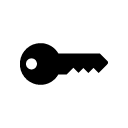
\includegraphics[scale=0.3]{img/key-128.png}};  
    \node (b) at (9.8,1) {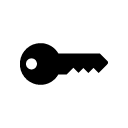
\includegraphics[scale=0.3]{img/key-128.png}};  
    \node (c) at (6,-1) {
\includegraphics[scale=0.05]{img/lock-128.png}};  
  \end{tikzpicture}
  \caption{The general strategy of a symmetric cryptography protocol.}
  \label{fig:crypto-sym}
\end{figure}
One famous example of an old cryptography protocol is the Caesar cipher, in
which each letter of the message is replaced by another letter. All the letters
are shifted by a constant number $n$ of positions down the alphabet. For
example, with $n=3$, the letter \texttt{D} becomes \texttt{A}, the letter
\texttt{E} becomes \texttt{B}, the letter \texttt{F} becomes \texttt{C}, and so
on. This encryption protocol is named after Julius Caesar,
who was using it to communicate with his generals with the shift $n=3$. In
Figure~\ref{fig:caesar}, we draw the correspondence between the letters using
the shift $n=3$. The outer ring represent the letters in the \emph{plaintext}
(the original text, without encryption) while the inner ring represent the
letters in the \emph{cyphertext} (the text after the encryption).
\begin{figure}[h]
  \centering
  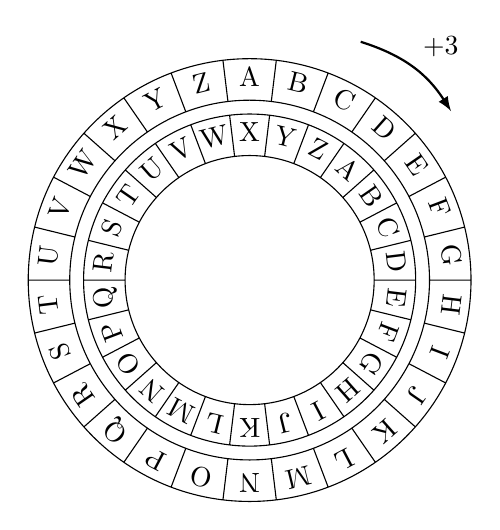
\begin{tikzpicture}[x=1em,y=1em]
%   set up
    \pgfmathsetmacro\angdiv{360/26}
    \pgfmathtruncatemacro\caeser{3} % Input Caeser shift here! (positive for clockwise)
    \coordinate (n-0) at (90+\angdiv/2:7) {};
    \coordinate (m-0) at (90-\caeser*\angdiv+\angdiv/2:5) {};
%   draw Caeser diagram
    \draw circle [radius=8] circle [radius=6.5] circle [radius=6]  circle [radius=4.5]
        \foreach \i in {0,...,25}{%
            ($({90-(\i-1/2)*\angdiv}:8)$) -- ($(({90-(\i-1/2)*\angdiv}:6.5)$)
            ($({90-(\i-1/2)*\angdiv}:4.5)$) -- ($(({90-(\i-1/2)*\angdiv}:6)$)
        };
    \foreach [count=\a from 0] \text in {A,B,...,Z}{
        \pgfmathtruncatemacro\b{\a+1}%
        \path [curved text=\text] (n-\a) arc [start angle=90-(\a-1/2)*\angdiv, delta angle=-\angdiv, radius=7] node (n-\b) {};
        \path [curved text=\text] (m-\a) arc [start angle=90-(\a+\caeser-1/2)*\angdiv, delta angle=-\angdiv, radius=5] node (m-\b) {}; % Inner circle
    }
%   draw arrow
    \draw [-latex, thick] (65:9.5) to[bend left=20,edge label=$+3$] (40:9.5);
    \end{tikzpicture}
  \caption{Representation of the Caesar cipher with a shift $n=3$.}
  \label{fig:caesar}
\end{figure}
In this example, the secret key of the protocol is the shift parameter $n$: if
you know $n$, you know both how to encrypt a message and how to decrypt one.
Caesar cipher is simple enough to be executed by a machine, but it is not used
nowadays. Indeed, the number of keys one can choose when using Caesar cipher is
rather small, so an adversary (a spy, an enemy...) can easily guess what it is
after spending enough time trying all the possibilities. One could even ask a
computer to search for all the possible keys, thus recovering it even faster.
That is why, in modern cryptography, the number of possible keys must be way
bigger than this. For example, the standard protocol for symmetric encryption,
called AES (for Advanced Encryption Standard), was designed in 1999~\cite{DR99,
DR02} and can be used with $2^{128}, 2^{192}$ or $2^{256}$ different possible
keys, depending on the version used. The smallest of these number can also be
written as
\[
  2^{128} = 340282366920938463463374607431768211456,
\]
when a billion looks like
\[
  10^{9} = 1000000000,
\]
so they are really big numbers.

The number of possible keys is not the only thing that changed since Julius
Caesar. First, communication is now essentially numerical, thus cryptography is
now a part of computer science. This is very important because it means that the
work in this thesis is also oriented towards computer science: we want to obtain
mathematical results that are effective, \ie usable by a computer.
Second, the scope of cryptography is now larger.
In modern cryptography, symmetric encryption is only one field of
cryptography, and there are many more aspects, such as asymmetric
encryption (also called \emph{public-key} encryption), data integrity,
anthentification, digital signatures (the list is not exhaustive). We will not
explain all these terms, but the interested reader can look at the introductions
on each of these subjects in~\cite{MVOV18}, for example. An important change in
cryptography occured in 1976 with the seminal article \emph{New Directions in
Cryptography}~\cite{DH76} by Diffie and Hellman, with the invention of so called
public key cryptography. We briefly present public key encryption, in order to
compare it to symmetric encryption.

One of the main drawback about symmetric encryption is that the two
protagonists must have a secret in common in order to be able to securely
communicate. They can meet in person and agree on a secret, but this is not
always possible, for example if they live very far away of each other. They
could also find another way of communication, but then they cannot encrypt their
communication, because they do not share a secret yet and they want to
communicate precisely in order to share one. Thus, the problem of sharing a
secret seems to be unsolvable. In fact, public key encryption is an answer to
this problem, because it allows to encrypt messages without the need for a
common secret. The elegant idea of Diffie and Hellman is to break the symmetry
between the participants (we will call them Alice and Bob, since it is
traditional to do so in cryptography). Instead of agreeing on a common key, only
one participant (for example Alice) creates a \emph{pair} of keys: one of them
is public and can be transmitted to anyone, while the other is private and must
be known by Alice only. With the public key, one can encrypt a message, while
the private key is necessary in order to decrypt an encrypted message. Using
such a system, everyone is able to send encrypted messages to Alice, because the
key used to do so is public, but only Alice can decrypt them. Thus, the
communications are secure.
\begin{figure}[h]
  \centering
  \begin{tikzpicture}
    \node (msg) at (0,0) {Message};
    \node (msg-enc) at (6,0) {Encrypted message};
    \node (msg-dec) at (12,0) {Decrypted message};
    \node (bob) at (0,2) {Bob};
    \node (alice) at (12, 2) {Alice};
    \node (key-pub) at (5, 2) {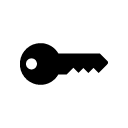
\includegraphics[scale=0.3]{img/key-128.png}};
    \node (key-pub-txt) at (5, 3) {Public key};
    \node (key-pri) at (7, 2) {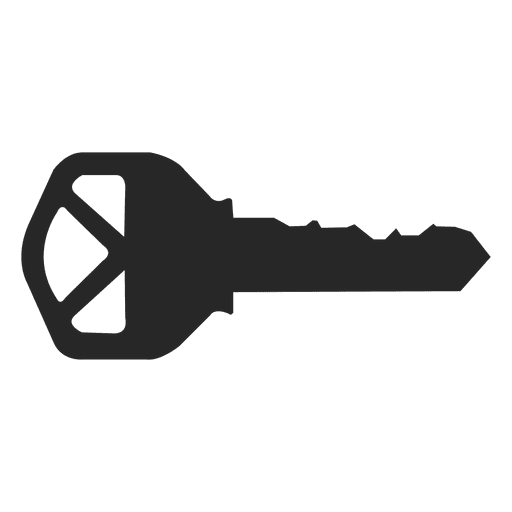
\includegraphics[scale=0.065]{img/key-512.png}};
    \node (key-pri-txt) at (7, 3) {Private key};
    \node (lock) at (6,-1) {
\includegraphics[scale=0.05]{img/lock-128.png}};  
    \draw[->] (msg) -- (msg-enc);
    \draw[->] (msg-enc) -- (msg-dec);
    \draw[->] (bob) to[bend left, edge label=Encrypts] (2.5,0);
    \node (key-pub2) at (2.2, .8) {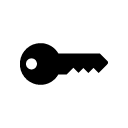
\includegraphics[scale=0.3]{img/key-128.png}};
    \draw[->] (alice) to[bend right, edge label = Decrypts] (9,0);
    \node (key-pri2) at (9.4, .8) {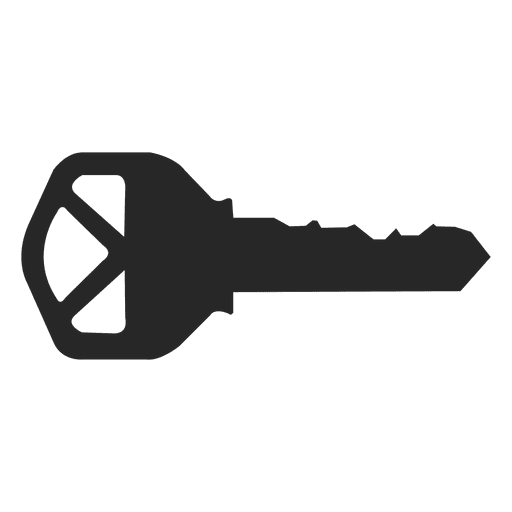
\includegraphics[scale=0.065]{img/key-512.png}};
    \draw[->] (alice) to (8,2);
    \node (c) at (9.5, 2.3) {Creates};
  \end{tikzpicture}
  \caption{General concept of public-key encryption.}
  \label{fig:crypto-asym}
\end{figure}
We dray a diagram of the general idea in Figure~\ref{fig:crypto-asym}. With such
a system, only Bob can send messages to Alice. If Alice wants to send a message
to Bob using public-key cryptography, then Bob has to create his own pair of
keys. He then gives his public key to Alice, that can then encrypt her message
using this key and send it to Bob. Bob decrypts the message using his private
key. Public-key cryptography is somewhat heavier than symmetric
cryptography, hence another solution for Bob is to encrypt a secret and send it
to Alice, in order to be able to use symmetric encryption with that secret. This
is what is done in practice: only a \emph{key exchange} is performed using
public-key cryptography, the rest being handled by symmetric cryptography.
Still, public-key cryptography is fundamental, since it allows us to use
symmetric cryptography.

The first key exchange protocol was invented by Diffie and Hellman in
1976~\cite{DH76}, and an example of public-key encryption is given by the RSA
(named after Rivest, Shamir, and Adleman) protocol~\cite{RSA78} that was
described in 1977. These two protocols are both based on mathematical algebraic
structures. Indeed, mathematics are a handy way of studying and explaining
cryptography, for example Caesar cipher with $n=3$ can be explained by
representing all letters by the numbers between $0$ and $25$
\[
  \texttt{A}\to 0, \texttt{B} \to 1, \dots,\texttt{Y}\to24, \texttt{Z}\to25
\]
and by defining the encryption as the substration by $3$. With this
representation, we have to agree that the number $-1$ is equivalent to the
number $25$, \ie before \texttt{A} comes \texttt{Z}, that $-2$ is equivalent to
$24$, \ie two times before \texttt{A} comes \texttt{Y}, and so on. In fact a
subpart of mathematics called \emph{number theory} is dedicated to the study of
this kind of numbers, together with some rules like the one that we just stated:
$-1=25$. These sets of numbers are called \emph{cyclic groups}, because they can
be represented on a circle, the one we spoke about is denoted by
\[
  \mathbb{Z}/26\mathbb{Z}
\]
and is represented in Figure~\ref{fig:cyclic-group}.
\begin{figure}[h]
  \centering
  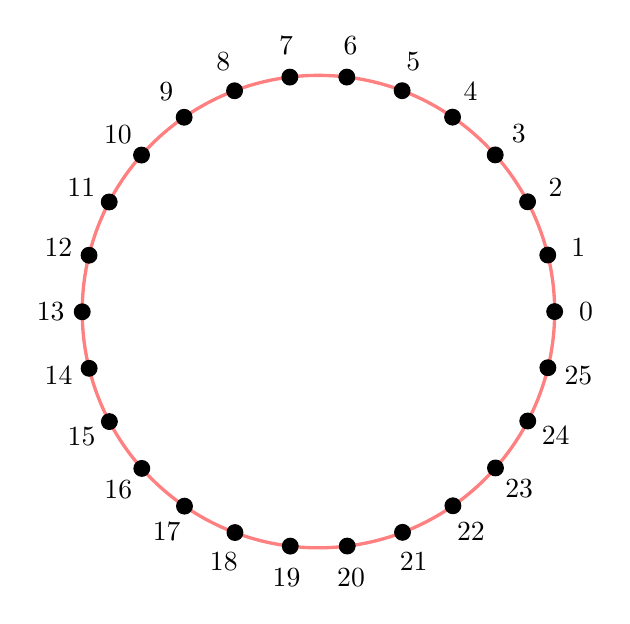
\begin{tikzpicture}
    \foreach \x in {0, 1,...,25} \coordinate (\x) at (13.85*\x:3);
    \draw[additive-structure] (0,0) circle (3);
    \foreach \x in {0, 1,...,25} \draw[fill] (13.85*\x:3) circle (.1);
    \foreach \x in {0, 1,...,25} \node (p) at (13.85*\x:3.4) {$\x$};
  \end{tikzpicture}
  \caption{The cyclic group $\mathbb{Z}/26\mathbb{Z}$ represented on a circle.}
  \label{fig:cyclic-group}
\end{figure}
Many other interesting structures exist, see for example~\cite{Lang04, Perrin96}
for a course in algebra. With the growth of public-key cryptography, number
theory became its corner stone, and more advanced mathematical concepts were
used, like finite fields, elliptic curves or isogenies. Without entering into
the details of what these objects are, what is important is that the security of
cryptographic protocols relies on hard mathematical problems involving these
concepts. Thus, a better understanding of them means a better understanding of
the security of our cryptographic protocols. The part of cryptography that is
dedicated to the study of the security of cryptographic protocols (\ie how to
``break'' them) is called \emph{cryptanalysis}.

At the same time, since the protocols are based on the manipulation of these
objects, a better understanding of them also means better (in particular,
faster) cryptographic protocols. Since cryptography is everywhere in modern
communications (on the Internet, when you use your credit card, on messaging
applications on your smartphone, ...), efficient protocols are crucial. It is
thus necessary to be able to efficiently manipulate the mathematical concepts
behind our protocols both for cryptography (making efficient protocols) and
cryptanalysis (being able to analyse their security). By ``manipulate'', we mean
being able to do additions, multiplications, and sometimes more complicated
operations with these objects: the science studying how to do so is called
\emph{arithmetic}. In conclusion, it is necessary to have efficient arithmetic
for cryptography and cryptanalysis.

\section{Finite fields arithmetic}

As stated in Section~\ref{sec:crypto}, cryptographic protocols rely on
mathematical structures in order to work. The one we will study during all this
document is called \emph{finite field}. A \emph{field} is a mathematical
structure (we also say \emph{algebraic structure}) composed of elements that we
can \emph{add}, \emph{substract}, \emph{multiply}, and \emph{divide} (except by
zero). It is a well-known algebraic structure: for example the set of real
numbers, denoted by $\mathbb{R}$, is a field. Indeed, the elements in
$\mathbb{R}$, for example $0, 1, -3, 5631$ but also more complicated numbers
such as $\pi, \sqrt 2, \frac{7}{13}$ can be added, substracted, multiplied or
divided. Numbers in $\mathbb{R}$ can have an infinite number of decimals, for
example the $60$ first decimals of the constant $\pi$ are
\[
  \pi = 3.14159265358979323846264338327950288419716939937510582097494\dots.
\]
A computer only has a finite memory, \ie the quantity of information it can
store is finite. As a consequence, it is impossible to store all the decimals of
$\pi$, and, more generally, the decimals of a lot of numbers in $\mathbb{R}$. It
is still possible to work with numbers in $\mathbb{R}$ on a computer, but it is
somewhat harder than to work with elements in a \emph{finite} algebraic
structure, \ie a set composed of $n$ elements, with
\[
  n < \infty.
\]
One example of such a structure was given in Section~\ref{sec:crypto}: the
cyclic groupe $\mathbb{Z}/26\mathbb{Z}$ that is composed of the ``numbers'' $0,
1, \dots, 25$. They are not the same numbers as those we know though, since with
the elements of $\mathbb{Z}/26\mathbb{Z}$ we have, for example
\[
  3 - 4 = -1 = 25,
\]
and this is not true for the actual numbers in $\mathbb{R}$, but we still write
them the same way for convenience. We already defined an
addition and substration on $\mathbb{Z}/26\mathbb{Z}$, and we could also define
a multiplication and a division in a very natural way. Finite fields are a
generalization of spaces like
$\mathbb{Z}/26\mathbb{Z}$. The set $\mathbb{Z}/26\mathbb{Z}$ is not a field for
technical reasons, but to think of finite fields as sets like this is a good
enough approximation for this introduction.

Because the elements of a finite fields are, by definition, finite, they are
somewhat easier to manipulate on a computer. Moreover, the field structure
allows us to manipulate the elements like usual numbers (\ie with additions,
multiplications, ...), which makes them useful. This is why today, finite fields
are everywhere in cryptography, but also in other domains at the crossroad of
mathematics and computer science, like coding theory.

Sometimes, simple mathematical problems are well understood on a theoretical
point of view, but there are still open questions concerning practical aspects.
For example, the multiplication of two integers $a$ and $b$ in $\mathbb{N}$ is a
simple problem, that can be done by hand by children. Still, the question of how
to compute it on a computer (in an optimal way) is open, and there are still
research articles~\cite{HVDH19} on that problem.
Finite field arithmetic (\ie how to perform operations such as additions and
multiplications) is very well understood, because the finite field structure is
rather simple. But again, the best way of multiplying two elements in a finite
field is still unknown. This is the subject of this thesis: the study of the
finite field arithmetic.

\section{Organization of the document}

This work is composed of two parts, that are essentially independent. In
Part~\ref{part:single}, we study the arithmetic of one fixed finite field
extension
\[
  \mathbb{F}_{p^k}.
\]
We begin in Chapter~\ref{chap:preliminary} by recalling fundamental
facts about the mathematical objects that we use in the rest of the document. We
review \emph{finite fields}, that are at the center of this thesis, and
\emph{algebraic function fields}, a concept that we use in proofs in
Chapters~\ref{chap:bilinear} and~\ref{chap:hypersymmetric}. We also
present the algebraic complexity model and some classic routines, that are
especially used in Chapters~\ref{chap:isomorphism} and~\ref{chap:standard}.

In Chapter~\ref{chap:bilinear}, we present the theory of \emph{bilinear
complexity}, an
alternative model of complexity used to measure the cost of computing bilinear
maps. We are in particular interested in the multiplication in finite field
extensions. We present an algorithm due to Chudnovsky and Chudnovsky~\cite{CC88}
that gives an asymptotic bound on the bilinear complexity of the product in
finite field extensions. Since this algorithm is not practical, we also give an
algorithm due to Barbulescu, Detrey, Estibal and Zimmermanm~\cite{BDEZ12} to
compute the bilinear complexity in small dimension.

In Chapter~\ref{chap:hypersymmetric}, we generalize the notion of bilinear
complexity to the product of $s\geq2$ variables
\[
  x_1\times x_2\times\dots\times x_{s-1}\times x_s
\]
in a finite field extension $\mathbb{F}_{p^k}$. We also generalize the fact
that this so called \emph{multilinear complexity} is still linear in the degree
$k$ of the extension~\cite{RR21}, as is the case with
the classic bilinear complexity. We define a new kind of complexity called the
\emph{hypersymmetric bilinear complexity}, that is inspired by the usual
symmetric bilinear complexity. We provide an \emph{ad hoc} algorithm to compute
this complexity in small dimension, and prove that it is still asymptotically
linear in the degree of the extension.

In Part~\ref{part:lattice}, we study how to deal with multiple finite fields
at once, in what we call a \emph{lattice of compatibly embedded finite fields}.
This is the equivalent as wondering how to compute in the algebraic closure
\[
  \bar{\mathbb{F}}_{p} = \bigcup_{k\geq1}\mathbb{F}_{p^k}
\]
of the base field $\mathbb{F}_p$. In Chapter~\ref{chap:isomorphism}, we review
the isomorphism problem, which asks how to efficiently compute an isomorphism
(or more generally an embedding)
\[
  K \emb L
\]
between two finite fields $K$ and $L$. We present the naive algorithm and the
Lenstra-Allombert algorithm~\cite{Lenstra91, Allombert02}. These algorithms will
respectively serve as the building blocks of the algorithms in
Chapters~\ref{chap:lattice} and~\ref{chap:standard}.

In Chapter~\ref{chap:lattice}, we present \emph{the compatibility problem}, that
asks how to compute embeddings between potentially much more that two finite
fields, in a compatible way, \ie so that the diagrams made of the embeddings
always commute. We present the Conway polynomials~\cite{Parker90, Scheerhorn92}
and the Bosma-Canon-Steel~\cite{BCS97}
framework, two different solutions for the compatibility problem. We also
provide an implementation~\cite{DRR18} of Bosma-Canon-Steel framework in
Nemo~\cite{Nemo}, a library of the Julia~\cite{Julia} programming language.

Finally, in Chapter~\ref{chap:standard}, we construct a new method~\cite{DRR19}
for computing lattices of compatibly embedded finite fields, that is halfway
between the Conway polynomials and the Bosma-Canon-Steel framework, and is
inspired by the Lenstra-Allombert embedding algorithm. We explain the benefits
of using this new method and provide an implementation in Julia, using Nemo.


\part{Efficient arithmetic in a single finite field}
\label{part:single}

\chapter{Preliminaries}
\label{chap:preliminary}
Throughout all this document, we will use a lot of results from algebra. This
chapter is here to sum up these results and try to maintain the illusion that
this thesis is self-contained. Our references for standard results in algebra
are~\cite{Lang04} or~\cite{Perrin96}.
The reader familiar with the notions of finite
fields, algebraic function fields, or complexity model may very well skip this
chapter.
\minitoc

\begin{figure}
  \centering
  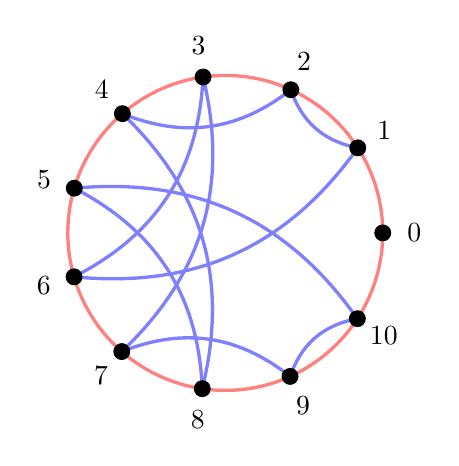
\begin{tikzpicture}
    \foreach \x in {0, 1,...,10} \coordinate (\x) at (32.7*\x:2);
    \draw[additive-structure] (0,0) circle (2);
    \draw[multiplicative-structure] (1) to [bend left] (2);
    \draw[multiplicative-structure] (2) to [bend left] (4);
    \draw[multiplicative-structure] (4) to [bend left] (8);
    \draw[multiplicative-structure] (8) to [bend right] (5);
    \draw[multiplicative-structure] (5) to [bend left] (10);
    \draw[multiplicative-structure] (10) to [bend right] (9);
    \draw[multiplicative-structure] (9) to [bend right] (7);
    \draw[multiplicative-structure] (7) to [bend right] (3);
    \draw[multiplicative-structure] (3) to [bend left] (6);
    \draw[multiplicative-structure] (6) to [bend right] (1);
    \foreach \x in {0, 1,...,10} \draw[fill] (32.7*\x:2) circle (.1);
    \foreach \x in {0, 1,...,10} \node (p) at (32.7*\x:2.4) {$\x$};
  \end{tikzpicture}
  \caption{Cyclic group structure of $(\mathbb{F}_{11}, +)$ (red) and
  $(\mathbb{F}_{11}^\times, \times)$ (blue).}
  \label{fig:finite-field}
\end{figure}
 
\clearpage
\section{Finite fields}

Finite fields are ubiquitous in cryptography and coding theory, probably because
their field structure, a rigid one, allows to understand how they work, and
their finiteness makes them easier to represent on a computer. They are also
everywhere in this thesis, and are probably on almost every paper I
wrote on during these last three years. They are quite important. A detailed
book about finite fields is~\cite{LN97}.

\subsection{Finite field structure}

A \emph{finite field} is a field $\K$ whose cardinality is finite. The first
examples of finite fields are the rings 
\[
  \mathbb{Z}/p\mathbb{Z}
\]
with $p\in\mathbb{N}$ a prime number. More generally, we denote by
$\mathbb{F}_{q}$ the finite field with $q$ elements. The cardinality of a finite
field is very well understood.
\begin{prop}
 There exists a unique (up to isomorphism) finite field of cardinality $q = p^l$
 for earch prime number $p\in\mathbb{N}$ and integer $l\geq1$.
\end{prop}
Let $q=p^l$ a prime power, there are several ways of representing
\emph{the} finite field with $q$ elements, but the one that we will almost
always have in mind is the following.

\begin{prop}
Let $P\in\mathbb{F}_p[x]$ be an
irreducible polynomial of degree $l$ with coefficients in $\mathbb{F}_p$. Then
\[
  \mathbb{F}_p[x]/(P(x))
\]
is a finite field with $q = p^l$ elements.
\end{prop}
We often write
\[
  \mathbb{F}_q \cong \mathbb{F}_{p}[x]/(P(x))\cong \mathbb{F}_p(\alpha)
\]
in order to say that we work with a finite field of $q$ elements, represented by
the quotient $\mathbb{F}_{p}[x]/(P(X))$, and where the projection of $x$ in the
quotient is denoted by $\alpha=\bar x$.

\subsection{Subfields and field extensions}

The finite field $\mathbb{F}_{p^l}$ is a
field extension of $\mathbb{F}_{p}$ of dimension $l$, \ie it is a
$\mathbb{F}_{p}$-vector space of dimension $l$. When dealing with the vector
space structure of $\mathbb{F}_{p^l}=\mathbb{F}_{p}(\alpha)$, we almost always choose to work with the
cannonical basis 
\[
  1, \alpha, \alpha^2, \dots, \alpha^{l-1}.
\]
Other interesting types of bases exist, such as for example normal
bases~\cite{Gao93}, but we always precise the basis when it is not clear from
the context.
Given $q=p^m$ a prime power and
$l\in\mathbb{N}$ an integer, we also write 
\[
  \mathbb{F}_{q^l}
\]
the field with $q^l = p^{ml}$ elements. We have
\[
  \mathbb{F}_{q^l}\cong\mathbb{F}_{p^{lm}},
\]
but the difference is that we see $\mathbb{F}_{q^l}$ as an extension of
$\mathbb{F}_{q}$ of dimension $l$, and not as an extension of the prime field
$\mathbb{F}_p$. Again, we usually think that our field $\mathbb{F}_{q^l}$ is
represented as
\[
  \mathbb{F}_{q^l}=\mathbb{F}_q[x]/(P(x)),
\]
where $P(x)\in\mathbb{F}_{q}[x]$ is an irreducible polynomial of degree $l$ with
coefficients in the base field $\mathbb{F}_q$. The subfields of
$\mathbb{F}_{q^l}$ are also well understood.
\begin{prop}
  \label{prop:subfields}
  Let $q=p^m$ be a prime power and $l\in\mathbb{N}$ an integer. Then there is
  an extension $\mathbb{F}_{q^m}$ of $\mathbb{F}_q$ of degree $m$ 
  included in $\mathbb{F}_{q^l}$
  \[
    \mathbb{F}_{q^m}\subset\mathbb{F}_{q^l}
  \]
  if and only if $m$ divides
  $l$. The elements in this subfield of $\mathbb{F}_{q^l}$ are the roots of the
  polynomial
  \[
    x^{q^m}-x
  \]
  in $\mathbb{F}_{q^l}$.
\end{prop}
Figure~\ref{fig:F12} describes the subfields of $\mathbb{F}_{12}$, as an
illustration of Proposition~\ref{prop:subfields}.
\begin{figure}
  \centering
  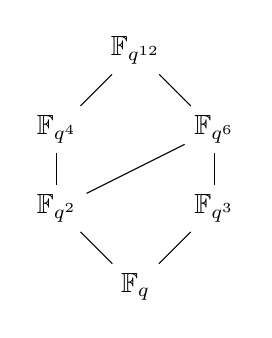
\begin{tikzpicture}
    \node (1) at (0,0) {$\mathbb{F}_{q}$}; 
    \node (2) at (-1,1) {$\mathbb{F}_{q^2}$}; 
    \node (3) at (1,1) {$\mathbb{F}_{q^3}$}; 
    \node (4) at (-1,2) {$\mathbb{F}_{q^4}$}; 
    \node (6) at (1,2) {$\mathbb{F}_{q^6}$}; 
    \node (12) at (0,3) {$\mathbb{F}_{q^{12}}$}; 
    \draw (1) -- (2);
    \draw (1) -- (3);
    \draw (2) -- (4);
    \draw (2) -- (6);
    \draw (3) -- (6);
    \draw (6) -- (12);
    \draw (4) -- (12);
  \end{tikzpicture}
  \caption{The subfields of $\mathbb{F}_{12}$. Two fields are linked if one is a
subfield of the other.}
  \label{fig:F12}
\end{figure}
The $\mathbb{F}_q$-automorphisms of the extension $\mathbb{F}_{q^l}$ are given
by the following result.
\begin{prop}
  Let $q=p^m$ be a prime power and $l\in\mathbb{N}$ an integer.
  The group of $\mathbb{F}_q$-automorphisms of $\mathbb{F}_{q^l}$ is a cyclic
  group of order $l$ generated by
  \[
    \sigma : t\mapsto t^q.
  \]  
\end{prop}
Let $u\in\mathbb{F}_{q^l}$, the conjugates of $u$ are the elements
\[
  \sigma(u), \sigma^2(u), \dots, \sigma^{l-1}(u)
\]
and the orbit of $u$ is the set
\[
  \left\{ u, \sigma(u), \dots, \sigma^{l-1} \right\}.
\]
This orbit might have any length $m$ dividing $l$. The orbit of $u$ is of length
$m$ if and only if $u$ is in a subfield $\mathbb{F}_{q^m}$ of
$\mathbb{F}_{q^l}$. We also sometimes write
\[
  u^\sigma = \sigma(u).
\]
Two maps, defined with the conjugates of a given element,
will play a very important role, the \emph{trace} and the \emph{norm}.
\begin{defi}[Trace and norm]
  Let $q$ a prime power and 
  \[
    \mathbb{F}_{q^l}/\mathbb{F}_q
  \]
  an extension of degree $l$, let $G$ be the group of
  $\mathbb{F}_q$-automorphisms of $\mathbb{F}_{q^l}$, and let
  $u\in\mathbb{F}_{q^l}$. Then the \emph{trace} of $u$ is
  \[
    \tr_{\mathbb{F}_{q^l}/\mathbb{F}_q}(u) = \sum_{\sigma\in G}u^\sigma
  \]
  and the \emph{norm} of $u$ is
  \[
    N_{\mathbb{F}_{q^l}/\mathbb{F}_q}(u)=\prod_{\sigma\in G}u^\sigma.
  \]
\end{defi}
We may only write $\tr$ or $N$ when the extension considered is clear from the
context. The trace over the field $\mathbb{F}_{q}$ is a $\mathbb{F}_{q}$-linear
map, and the norm is a multiplicative map, they are also both \emph{transitive},
as described in the next proposition.
\begin{prop}
  Let $q\in\mathbb{N}$ a prime power and $a\,|\,b\,|\,c$ three integers, giving
  the tower of extensions that follows.
  \begin{center}
  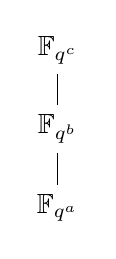
\begin{tikzpicture}
    \node (a) at (0,0) {$\mathbb{F}_{q^a}$}; 
    \node (b) at (0,1) {$\mathbb{F}_{q^b}$}; 
    \node (c) at (0,2) {$\mathbb{F}_{q^c}$}; 
    \draw (a) -- (b);
    \draw (b) -- (c);
  \end{tikzpicture}
  \end{center}
  Let $u\in\mathbb{F}_{q^c}$, then
  \[
    \tr_{\mathbb{F}_{q^c}/\mathbb{F}_{q^a}}(u) =
    \tr_{\mathbb{F}_{q^b}/\mathbb{F}_{q^a}}(\tr_{\mathbb{F}_{q^c}/\mathbb{F}_{q^b}}(u))
  \]
  and
  \[
    N_{\mathbb{F}_{q^c}/\mathbb{F}_{q^a}}(u) =
    N_{\mathbb{F}_{q^b}/\mathbb{F}_{q^a}}(N_{\mathbb{F}_{q^c}/\mathbb{F}_{q^b}}(u)).
  \]
\end{prop}
Finally, the map
\[
  (x, y)\mapsto\tr(xy)
\]
is a non-degenerate bilinear map that we will also sometimes write as
\[
  \ps{x}{y} = \tr(xy).
\]
%
%\subsection{Kummer extensions}
%
%Kummer extensions are a particular kind of extension, they play a special role in
%our construction of lattices of extension presented in
%Chapter~\ref{chap:lattice}. We follow the presentation of~\cite{Lang04}.

\section{Algebraic function fields}
\label{sec:algebraic-function-fields}

% Contents
% ========
%
% - algebraic function field
% - place
% - degree of a place
% - divisor
% - big theorems
% - definition of the genus ?

Together with algebraic curves, algebraic function fields are a way of
describing the algorithms of Chapters~\ref{chap:bilinear}
and~\ref{chap:hypersymmetric}. In this document, we choose to use the algebraic
function field point of view. The function fields we need are constructed
on top of finite fields, so we present the theory with that context in mind. For
this section, our reference is~\cite{Stichtenoth09}. In all the section, $\K$ is
a finite field of characteristic $p$.

\subsection{Places}

Let us first define what an algebraic function field is, together with important
notions leading to the definition of \emph{places}.
\begin{defi}[Algebraic function field]
  An \emph{algebraic function field} $F$ of one variable over $\K$ is an
  extension field 
  \[
    F/\K
  \]
  such that $F$ is a finite algebraic extension of
  $\K(x)$ for some element $x\in F$ which is transcendental over $\K$.
\end{defi}
From now on, the notation $F$ will represent an algebraic function field over
$\K$. Since it is not critical to the theory, we also assume that $\K$ is
algebraically closed in $\K$ for simplicity.

\begin{defi}[Valuation ring]
  A \emph{valuation ring} $\vr$ of the function field $F/\K$ is a ring 
  \[
    \vr \subset F
  \]
  with the following properties
  \begin{enumerate}
    \item $\K\subsetneq\vr\subsetneq F$;
    \item for all $z\in F$, we have $z\in\vr$ or $z^{-1}\in\vr$.
  \end{enumerate}
\end{defi}
\begin{prop}
  \label{prop:valring}
Let $\vr$ be the a valuation ring of the function field $F$. 
\begin{enumerate}[(a)]
    \item The ring $\vr$ is local, \ie it has a unique maximal ideal that is given
      by
      \[
        P = \vr\setminus\vr^\times
      \]
      where $\vr^\times$ is the group of units of the ring $\vr$.
    \item \label{cond:valring} For any nonzero $x\in F$, we have
      \[
        x\in P\Longleftrightarrow x^{-1}\notin\vr.
      \]
\end{enumerate}
\end{prop}
\begin{thm}
  \label{thm:discrete-valring}
 Let $\vr$ be the valuation ring of the function field $F$ and $P$ be its unique
 maximal ideal. Then
 \begin{enumerate}[(a)]
   \item The ideal $P$ is principal.
   \item If $P=t\vr$ then any nonzero $z\in F$ has a unique representation of
     the form
     \[
       z = t^n u
     \]
     with $n\in\mathbb{Z}$ and $u\in\vr^\times$
   \item The ring $\vr$ is a principal ideal domain. More precisely, if $P=t\vr$
     and
     \[
       \left\{ 0 \right\}\neq I\subseteq\vr
     \]
     is an ideal then
     \[
       I = t^n\vr
     \]
     for some $n\in\mathbb{N}$.
 \end{enumerate}
\end{thm}
A ring having the properties described in Theorem~\ref{thm:discrete-valring} is
called a \emph{discrete valuation ring}.
\begin{defi}[Place]
  A \emph{place} $P$ of $F$ is the maximal ideal of some valuation ring $\vr$ of $F$.
\end{defi}
\begin{defi}[Prime element]
  Let $\vr$ be a valuation ring and $P$ its maximal ideal. Any element $t\in P$
  such that
  \[
    P = t\vr
  \]
  is called a \emph{prime element} for $P$. It is also sometimes called a
  \emph{local parameter} or a \emph{uniformizing variable}.
\end{defi}
If $\vr$ is a valuation ring of $F$ and if $P$ is its maximal ideal, then $\vr$
is uniquely determined by $P$, indeed we have
\[
  \vr = \left\{ z\in F\mid z^{-1}\notin P \right\}
\]
thanks to Proposition~\ref{prop:valring}\ref{cond:valring}. Thus, the notions of
valuation rings and places are essentially equivalent. There is a third way of
describing a place, given by discrete valuations.
\begin{defi}[Discrete valuation]
  A \emph{discrete valuation} of $F$ is a function
  \[
    v:F\to\mathbb{Z}\cup\left\{ \infty \right\}
  \]
  with the following properties:
  \begin{enumerate}
    \item $v(x) = \infty \Leftrightarrow x=0$;
    \item for any $x,y\in F$, $v(xy) = v(x)+v(y)$;
    \item for any $x,y\in F$, $v(x+y)\geq\min(v(x), v(y)$;
    \item there exists an element $z\in F$ with $v(z)=1$;
    \item for any nonzero element $a\in\K$, $v(a) = 0$.
  \end{enumerate}
\end{defi}
Here, the symbol $\infty$ means an element that is not in $\mathbb{Z}$, such
that $\infty+\infty = \infty + n = \infty$ and $\infty > m$ for any
$m,n\in\mathbb{Z}$.
\begin{defi}
  To any place $P\in\mathbb{P}_F$, we associate a function
  \[
    v_P:F\to\mathbb{Z}\cup\left\{ \infty \right\}
  \]
  that is in fact a discrete valuation ring. Let $t$ be a prime element for $P$.
  Then every nonzero element $z\in F$ has a unique representation
  \[
    z = t^n u
  \]
  with $u\in\vr^\times$ and $n\in\mathbb{Z}$. We define
  \[
    v_P(z)\eqdef n
  \]
  and
  \[
    v_P(0)\eqdef\infty.
  \]
\end{defi}
This definition does not depend on the prime element $t$ that was chosen. It
allows us to give the third equivalent way of describing a place of $F$.
\begin{thm}
 Let $F$ be a function field.
 \begin{enumerate}[(a)]
   \item For any place $P\in\mathbb{P}_F$, the function $v_P$ defined above is a
     discrete valuation of $F$. Moreover, we have
     \begin{align*}
       \vr_P &= \left\{ z\in F\mid v_P(z)\geq0 \right\},\\
       \vr_P^\times &= \left\{ z\in F\mid v_P(z)>0 \right\},\\
       P &= \left\{ z\in F\mid v_P(z)=0 \right\}.
     \end{align*}
     An element $x\in F$ is a prime element for $P$ if and only if $v_P(x)=1$.
   \item Conversely, if $v$ is a discrete valuation of $F$, then the set
     \[
       P = \left\{ z\in F\mid v(z)>0 \right\}
     \]
     is a place of $F$, and
     \[
       \vr_P = \left\{ z\in F\mid v(z)\geq0\right\}
     \]
     is the corresponding valuation ring.
 \end{enumerate}
\end{thm}
We let $\mathbb{P}_F$ be the set of places of $F$. If $P\in\mathbb{P}_F$ is a
place of $F$, we denote by $\vr_P$ the corresponding valuation ring. Since $P$
is a maximal ideal of $\vr$, we also know that the quotient ring
\[
  F_P = \vr_P/P
\]
is a field. We call this field $F_P$ the \emph{residue class field} of $P$.
\begin{defi}[Residue class map]
Let $P\in\mathbb{P}_F$ be a place of $F$. For $x\in F$, we let 
\[
  x(P)
\]
be the residue class of $x$ modulo $P$. If $x\notin \mathcal O_P$, we define $x(P)=\infty$.
The map from $F$ to $F_P\cup\left\{ \infty \right\}$
\[
  x\mapsto x(P)
\]
is called the \emph{residue class map}.
\end{defi}
\begin{defi}[Degree of a place]
  Let $P\in\mathbb{P}_F$ a place of $F$. The residue class field $F_P$ is a
  finite extension of $\K$ and we call
  \[
    \deg P = \left[ F_P\,:\,\K \right]
  \]
  the \emph{degree} of $P$.
\end{defi}
In fact, the degree of a place if always finite. If $P$ is a place of degree
$1$, then its residue class field $F_P$ is equal to
\[
  F_P = \K.
\]
The residue class map then maps $F$ to $\K\cup\left\{ \infty \right\}$. In
particular, if $\K$ is algebraically closed, any place has degree $1$, thus we
can interpret an element $z\in F$ as a function
\[
  \begin{array}{cccc}
    z:&\mathbb{P}_F&\to&\K\cup\left\{ \infty \right\}\\
    & P & \mapsto & z(P)
  \end{array}.
\]
This justifies the name \emph{function field} for $F$. With this interpretation,
places of degree $1$ are viewed as points and elements in $\K$ are viewed as
constant functions. This is also a reason behing the following terminology.
\begin{defi}[Zero and pole]
  Let $z\in F$ be an element in the function field $F$ and $P\in\mathbb{P}_F$ a
  place of $F$. We say that $P$ is a \emph{zero} of $z$ if $v_P(z)>0$ and that
  $P$ is a \emph{pole} of $z$ if $v_P(z)<0$. If $v_P(z) = n > 0$, then $P$ is a
  \emph{zero of order} $n$; if $v_P(z) = -n < 0$, then $P$ is a \emph{pole of
  order} $n$.
\end{defi}
Note that if $P$ is a zero of $z\in F$, we have $z(P) = 0$, while we have
$z(P)=\infty$ if $P$ is a pole of $z$. Another important results states that
every element not in $\K$ yields a non-constant function.
\begin{prop}
 Let $F$ be a function field and $z\in F$ an element in $F$ that is
 not in $\K$. Then $z$ has at least one zero and one pole. In particular, this
 proves that the set $\mathbb{P}_F$ of places is not empty.
\end{prop}

\subsection{Independence of valuations}

Before talking about the central notions of divisors and Riemann-Roch spaces, we
must mention one important theorem called the \emph{weak approximation theorem}
(also reffered to as \emph{theorem of independence}). It essentially says that
if we have pairwise distinct discrete valuations $v_1, \dots, v_n$ of $F$ and an
element $z\in F$ for which we know the values $v_1(z), \dots, v_{n-1}(z)$, then
we cannot conclude anything about the value $v_n(z)$.
\begin{thm}
  \label{thm:weak-approx}
  Let $F$ be a function field, $P_1, \dots, P_n\in\mathbb{P}_F$ be pairwise
  distinct places of $F$, $x_1, \dots, x_n\in F$ be elements in $F$ and $r_1,
  \dots, r_n\in\mathbb{Z}$ be integers. Then there is some $x\in F$ such that
  \[
    v_{P_i}(x-x_i) = r_i\text{ for all }1\leq i\leq n.
  \]
\end{thm}
The name ``approximation theorem'' comes from the fact that $v_{P_i}(x-x_i)$ can
be interpreted as some ``distance'' between $x$ and $x_i$. With this
interpretation, Theorem~\ref{thm:weak-approx} says that the distances between
$x$ and $x_i$ can be made simultaneously arbitrarily small using \emph{one}
element $x$. This theorem allows us to mention important results.
\begin{cor}
  Any function field $F$ has infinitely many places.
\end{cor}
\begin{prop}
  Let $F$ be a function field and $P_1, \dots, P_r$ be the zeros of some element
  $x\in F$. Then
  \[
    \sum_{i=1}^r{v_{P_i}(x)\cdot\deg P_i}\leq \left[ F:\K(x) \right].
  \]
\end{prop}
\begin{cor}
  In a function field $F$, any nonzero element $x\in F$ has only finitely many
  zeros and poles.
\end{cor}

\subsection{Divisors}

Now that we now what places are, we can define divisors. In this section, we
keep the notation of last section: we let $F$ be an algebraic function field
over a finite field $\K$ of characteristic $p$.
\begin{defi}[Divisor]
  The \emph{divisor group} $\Div(F)$ of $F$ is defined as the free abelian group generated
  with the places of $F$. The elements of $\Div(F)$ are called the
  \emph{divisors} of $F$. In other words, a divisor is a formal sum
  \[
    D = \sum_{P\in\mathbb{P}_F} n_P\cdot P
  \]
  with $n_P\in\mathbb{Z}$ and $n_P=0$ for all but finitely many places $P$.
\end{defi}
\begin{defi}[Support]
  Let 
  \[
    D = \sum_{P\in\mathbb{P}_F} n_P\cdot P
  \]
  be a divisor of $F$. We define the \emph{support} of $D$ as
  \[
    \supp D = \left\{ P\in\mathbb{P}_F\,|\,n_P\neq 0 \right\}.
  \]
\end{defi}
Two divisors 
\[
  D = \sum_{P\in\mathbb{P}_F} n_P\cdot P
\]
and
\[
  D' = \sum_{P\in\mathbb{P}_F} n_P'\cdot P
\]
in $\Div(F)$ are added coefficient-wise:
\[
  D+D' = \sum_{P\in\mathbb{P}_F} (n_P+n_P')\cdot P
\]
and the zero element is the divisor
\[
  0 \eqdef \sum_{P\in\mathbb{P}_F} n_P\cdot P
\]
with $n_P=0$ for all places $P\in\mathbb{P}_F$. If
\[
  D = \sum_{P\in\mathbb{P}_F}n_P\cdot P
\]
is a divisor $\Div(F)$ and $Q\in\mathbb{P}_F$ is a place of $F$, we let 
\[
  v_Q(D) = n_Q
\]
be the coefficient multiplying $Q$ in the formal sum $D$. We then have
\[
  \supp D = \left\{ P\in\mathbb{P}_F\mid v_P(D)\neq 0 \right\}.
\]
We then define a partial ordering on $\Div(F)$ by
\[
  D_1 \leq D_2 \overset{\text{def}}{\Longleftrightarrow} v_P(D_1)\leq v_P(D_2)\text{ for all
  }P\in\mathbb{P}_F.
\]
A divisor $D\geq 0$ is called \emph{positive} (or \emph{effective}).
\begin{defi}[Degree]
  Let $D\in\Div(F)$ be a divisor, its \emph{degree} is defined by
  \[
    \deg(D) = \sum_{P\in\mathbb{P}_F}v_P(D)\deg(P)
  \]
  and yields a homomorphism $\deg:\Div(F)\to\mathbb{Z}$.
\end{defi}
\begin{defi}
  Let $x\in F$ be a nonzero element in $F$, $Z\subset\mathbb{P}_F$ be the set of
  its zeros and $N\subset\mathbb{P}_F$ be the set of its poles. Then, we define
  \begin{align*}
    (x)_0 &= \sum_{P\in Z}v_P(x)P ,\,\text{ the \emph{zero divisor} of }x,\\
    (x)_\infty &= \sum_{P\in N}(-v_P(x))P ,\,\text{ the \emph{pole divisor} of
  }x,\\
    (x) &= (x)_0 - (x)_\infty ,\,\text{ the \emph{principal divisor} of }x.
  \end{align*}
\end{defi}
We have $(x)_0\geq0, (x)_\infty\geq0$ and
\[
  (x) = \sum_{P\in\mathbb{P}_F}v_P(x)P.
\]
If $x\in K$, then $x$ does not have zeros nor poles and the sum is then empty,
conversely a function in $F\setminus\K$ has at least one zero and one pole, we
thus have
\[
  x\in\K\Leftrightarrow (x)=0.
\]
\begin{defi}[Equivalence]
  Let $D, D'\in\Div(F)$ be two divisors of $F$. We can define an equivalence
  relation by
  \[
    D\sim D'\Longleftrightarrow\text{ there exists }x\in F\text{ such that }D =
    D'+(x).
  \]
  In that case, we say that $D$ and $D'$ are \emph{equivalent}.
\end{defi}
Principal divisors play a crucial role in the algebraic function field theory.
They allow us to define spaces that play a fundamental role.
\begin{defi}
  Let $D\in\Div(F)$ be a divisor of $F$. We let
  \[
    L(D) = \left\{ x\in F\mid(x)\geq -D \right\}\cup\left\{ 0 \right\}.
  \]
\end{defi}
This definition can be interpreted in the following way: if
\[
  D = \sum_{i=1}^rn_iP_i - \sum_{j=1}^sm_jQ_j,
\]
with $n_i>0$ and $m_j>0$, then $L(D)$ consists of all elements $x\in F$ such
that
\begin{enumerate}
  \item for all $1\leq j\leq s$, $x$ has a zero of order at least $m_j$ at $Q_j$;
  \item the places $P_1, \dots, P_r$ are the only poles of $x$, and for all
    $1\leq i\leq r$, the order of the pole $P_i$ is bounded by $n_i$.
\end{enumerate}
We recall some properties of the spaces $L(D)$ in
Proposition~\ref{prop:LD-spaces}.
\begin{prop}
  \label{prop:LD-spaces}
 Let $D\in\Div(F)$ be a divisor.
 \begin{enumerate}[(a)]
   \item $L(D)$ is a finite-dimensionnal $\K$-vector space.
   \item $L(D)\neq\left\{ 0 \right\}$ if and only if there exists a divisor
     $D'\sim D$ with $D'\geq0$.
   \item If $D'\sim D$, then $L(D)$ and $L(D')$ are isomorphic as $\K$-vector
     spaces.
   \item $x\in L(D)$ if and only if $v_P(x)\geq - v_P(D)$ for all
     $P\in\mathbb{P}_F$.
   \item $L(0)=\K$.
   \item If $\deg(D)<0$ then $L(D)=\left\{ 0 \right\}$. In particular if $D<0$
     then $L(D)=\left\{ 0 \right\}$.
 \end{enumerate}
\end{prop}
\begin{defi}[Dimension]
  Let $D\in\Div(F)$ be a divisor of $F$. The \emph{dimension} of $D$ is denoted
  by $\ell(D)$ and is defined by
  \[
    \ell(D) = \dim L(D).
  \]
\end{defi}
We can now define the most important invariant of a function field $F$, its
\emph{genus}.
\begin{defi}[Genus]
  Let $F$ be a function field. The \emph{genus} $g$ of $F$ is the nonnegative
  integer defined by
  \[
    g = \max\left\{ \deg D-\ell(D)+1\mid D\in\Div(F) \right\}.
  \]
\end{defi}
\begin{defi}[Index of specialty]
  Let $D\in\Div(F)$ be a divisor of $F$, the nonnegative integer
  \[
    i(D) = \ell(D) - \deg(D) + g - 1
  \]
  is called the \emph{index of specialty} of $D$. A divisor $D$ such that
  $i(D)=0$ is called \emph{non-special}; a divisor $D$ such that $i(D)>0$ is
  called \emph{special}.
\end{defi}
\begin{defi}[Canonical divisor]
  Let $F$ be a function field of genus $g$. A divisor $W$ of degree $\deg W = 2g-2$ and
  dimension $\ell(W) = g$ is called a \emph{canonical divisor}.
\end{defi}
In fact, all canonical divisors are equivalent, and they are involved in the
very important Riemman-Roch theorem.
\begin{thm}[Riemann-Roch]
  Let $W\in\Div(F)$ be a canonical divisor of $F$. Then, for any divisor
  $D\in\Div(F)$, we have
  \[
    \ell(D) = \deg(D) + 1 - g + \ell(W-D).
  \]
\end{thm}

\section{Complexity models}
\label{sec:complexity-models}

When studying algorithms, it is of central interest to understand how our algorithms
\emph{scale}, \ie to understand how they perform if the size of the input is
getting larger and larger. Complexity theory studies this phenomenon and gives us models
of computation in order to quantify the behaviour of our algorithms. Depending
on the situation, not all models are relevant, and one has to balance between
the concreteness of a model and its ease of use. An extreme viewpoint is to
specify an operating system with a compiled programming language and to compare
the running time or the memory requirements between algorithms. The advantage of
such a model is that it is very concrete, but it is also its main disadvantage
because it makes the model hard to use. Thus, there exist other models of
\emph{idealized} computers, such as Turing machines~\cite{Papadimitriou03},
random access machines, or the algebraic complexity model.
We use the latter, that we present in more details in the next section.

\subsection{Algebraic complexity}
\label{sec:algebraic-complexity}

This model is widely presented in~\cite{BCS13}, we only give a brief
presentation of the subject. This model assumes that we use an abstract computer
that is able to perform operations in some base field $\K$ at a constant, unit
cost. We also assume that accessing the memory of the computer is free.
Algebraic complexity is especially useful with algorithms dealing with
algebraic structures. This is very handy for us, since
we usually work with algebras
\[
  (\A, +, \times, \cdot)
\]
over some base field $\K$. As an example, with this model, the complexity of an
addition in the extension field
\[
  \mathbb{F}_4 = \mathbb{F}_2[T]/(T^2+T+1) = \mathbb{F}_2(x)
\]
where $x=\bar T$, if elements are represented in the basis $\left\{ 1, x
\right\}$, is $2$, because we only need $2$ additions in $\mathbb{F}_2$ to
perform an addition in $\mathbb{F}_4$. Indeed, if
\[
  a = a_0 + a_1x\in\mathbb{F}_4
\]
and
\[
  b = b_0 + b_1x\in\mathbb{F}_4,
\]
we have
\[
  a+b = (a_0+b_0)+(a_1+b_1)x.
\]
In the case of a multiplication, we have
\[
  ab = (a_0b_0+a_1b_1) + (a_0b_1+a_1b_0)x,
\]
so the complexity of a multiplication in $\mathbb{F}_4$ (at least with this
formula) is $6$, because we need
$4$ multiplications and $2$ additions in $\mathbb{F}_2$. In the context of
finite fields, it makes sense to consider that the cost of an operation is
independent of the operands, because the elements have a fixed size; but this is
no longer the case in other rings, for example in $\mathbb{Z}$, $\mathbb{Q}$,
$\mathbb{R}$, or $\mathbb{C}$. We could also argue that the different operations
in $\K$ should not have the same cost, we thus present an other manner of
computing the complexity of an algorithm, that is called \emph{bilinear
complexity}, in Chapter~\ref{chap:bilinear}.

\subsection{Landau notations}

In order to describe the asymptotic behaviour of an algorithm, we use the
classical \emph{big O} and \emph{little o} notations $O$ and $o$. Let $f:\mathbb{R}\to\mathbb{R}$ and
$g:\mathbb{R}\to\mathbb{R}$ be two functions, we write
\[
  f(x) = O(g(x))
\]
if there exist $M\in\mathbb{R}$ and $C>0$ such that
\[
  \forall x\geq M,\,|f(x)|\leq Cg(x).
\]
and we write
\[
  f(x)=o(g(x))
\]
if there exist $M\in\mathbb{R}$ and $\varepsilon:\mathbb{R}\to\mathbb{R}$, a
function with $\varepsilon(x)\to 0$ when $x\to\infty$, such
that
\[
  \forall x\geq M,\,|f(x)|\leq \varepsilon(x)g(x).
\]
We say that $f$ is equivalent to $g$ and we write
\[
  f(x)\sim g(x)
\]
if 
\[
 f(x)-g(x) = o(g(x))
\]
when $x\to\infty$. Finally, we also use the \emph{soft O} notation $\tilde{O}$ to neglect
logarithmic factors in the big O notation, we write
\[
  f(x) = \tilde{O}(g(x))
\]
if there exist some $k$ with $f(x) = O(g(x)\log^k(g(x)))$.

\section{Fundamental algorithms}

In this section, we briefly review the fundamental algorithms that are used in
the thesis. Unless explicitely stated otherwise, we measure the complexities
using the algebraic complexity presented in
Section~\ref{sec:algebraic-complexity}, \ie in number of operations $+, \times,
\div$ in some base field $\K$. References for this section are~\cite{GG13,
BCGLLSS17, BDDFS17}.

\subsection{Finite field arithmetic}

Since finite fields are so important in this thesis, we first review the
complexity of the basic operations in finite fields. We let
\[
  \K = \mathbb{F}_q
\]
be the finite field with $q$ elements, where $q$ is a prime power and we let $p$
be the characteristic of $\K$. We consider $\mathbb{F}_{q^n}$ a finite field
extension of degree $n$ of $\K$, and we assume that the elements in
$\mathbb{F}_{q^n}$ are represented by univariate polynomials in $\K\left[ x
\right]$. We let $P\in\K\left[ x \right]$ be the irreducible polynomial
defining $\mathbb{F}_{q^n}$, \ie we have
\[
  \mathbb{F}_{q^n} = \K\left[ x \right]/(P(x)).
\]
Then, the cost of the operations in $\mathbb{F}_{q^n}$ are those of polynomial
operations modulo $P$ in $\K\left[ x \right]$ and depend on polynomial
arithmetic. We let $M(n)$ be a function such that polynomials in $\K\left[ x
\right]$ of legree less than $n$ can be multiplied in $M(n)$ operations in $\K$.
We assume that the function $M$ has the \emph{superlinearity}
property~\cite[Chapter 8.3]{GG13}, \ie that for any $m,
n\in\mathbb{N}\setminus\left\{ 0 \right\}$, we have
\[
  \left\{
  \begin{array}{l}
    M(mn) \geq mM(n) \\
    M(n+m)\geq M(m) + M(n) \\
    M(n) \geq n
  \end{array}
  \right.
.\]
We also assume that $M(mn)$ is in $O(m^{1+\varepsilon}M(n))$ for all
$\varepsilon>0$. Using Fast Fourrier Transform~\cite{CT65, SS71}, Cantor and
Kaltofen~\cite{CK91} then proved that we have
\[
  M(n)\in O(n\log(n)\log\log(n)).
\]
Linear algebra operations play an important role too. We denote by $\omega$ the
\emph{exponent of linear algebra}, \ie a constant such that $n\times n$ matrices
in any field $\K$ can be multiplied using $O(n^\omega)$ additions and
multiplications in $\K$. One can take
\[
  \omega < 2.37286
\]
using~\cite{AW21}; on the other hand, we also suppose that $\omega >2$. The
algorithms achieving the best asymptotic complexity for matrix multiplications
are not practical, thus when estimating the complexity of algorithms we
sometimes take $\omega=3$, the complexity coming from the usual formula for
matrix multiplication, or $\omega\approx 2.807$ using Strassen's
algorithm~\cite{Strassen69}.

Adding two elements in $\mathbb{F}_{q^n}$ takes $O(n)$ additions in $\K$.
Similarly, adding two polynomials of degree up to $s$ in $\mathbb{F}_{q^n}\left[
T \right]$ takes $O(s)$ additions in $\mathbb{F}_{q^n}$, thus takes $O(sn)$
additions in $\K$. Multiplying and dividing polynomials of degree at most $s$ in
$\mathbb{F}_{q^n}$ in $\mathbb{F}_{q^n}\left[ T \right]$ is done in $O(M(sn))$
operations in $\K$, using Kronecker's substitution~\cite{Moenck76, Kaltofen87,
GG13, GS92, Harvey09}. If $h(T)\in\mathbb{F}_{q^n}[T]$ is a monic polynomial,
multiplication in $\mathbb{F}_{q^n}[T]/(h(T))$ is also done in $O(M(sn))$, using
the technique in~\cite{PS06}. In particular, this means that multiplication in
$\mathbb{F}_{q^n}$ costs $O(n)$ operations in $\K$. Using the same techniques,
the greater common divisor (gcd) of degree $s$ polynomials in
$\mathbb{F}_{q^n}[T]$ and inverses in $\mathbb{F}_{q^n}[T]/(h(T))$ can be
computed using $O(M(sn)\log(sn))$ operations in $\K$. Again, this means that
inverses in $\mathbb{F}_{q^n}$ can be computed using $O(M(n)\log(n))$
operations in $\K$.

\subsection{Classic routines}

We now give a few standard routines that are used in a lot of algorithms
involving finite fields, for example the algorithms presented in
Chapters~\ref{chap:isomorphism} and~\ref{chap:standard} extensively use these
routines.
Given polynomials $e, g, h\in\mathbb{F}_{q^n}[T]$ of degree at most $s$, the
modular composition is the problem of computing
\[
  e(g(T))\mod h(T).
\]
An upper bound on the algebraic complexity is obtained using the Brent-Kung
algorithm~\cite{BK78}. Following our discussion on the costs of polynomial
and matrix multiplication, its cost is $O(s^{(\omega+1)/2M(n)})$ operations in
$\K$. In the binary RAM complexity model, the Kedlaya-Umans
algorithm~\cite{KU11} and its extension~\cite{PS13} yield an algorithm with
essentially linear complexity in $s, n$ and $\log(q)$. Unfortunately, these
algorithms prove to be hard te implement in a competitive way, and Brent and
Kung's algorithm seem to outperform them in practice.

By applying transposition techniques~\cite{BLS03, DeFeo10, DS10, BCS13} to Brent
and Kung's algorithm, Shoup~\cite{Shoup94, Shoup99} derived an algorithm to
compute the minimal polynomial (over $\K$) of an element in $\mathbb{F}_{q^n}$
using $O(n^{(\omega+1)/2})$ operations in $\K$. We say a bit more about these
techniques, called \emph{transposition principle} (or \emph{Tellegen's
principle}) in Section~\ref{sec:modular-composition}.

We also sometimes use Berlekamp-Massey algorithm in order to compute the minimal
generating polynomial of a recurring sequence. Berlekamp-Massey algorithm takes
as input the $2n$ first terms $a_0, \dots, a_{2n-1}\in\K$ of a reccuring
sequence for which we know that the minimal generating polynomial has its degree
bounded by $n$. Using rational reconstruction~\cite[Chapter 7]{BCGLLSS17},
Berlekamp-Massey algorithm outputs the minimal generating polynomial of the
sequence $a_0, \dots, a_{2n-1}$ using $O(M(n)\log(n))$ operations in $\K$.


\chapter{Bilinear complexity and Chudnosky$^2$-type algorithms}
\label{chap:bilinear}
We have presented in Section~\ref{sec:complexity-models} an abstract model made
to understand the asymptotic behaviour of our algorithms. In this chapter, we
present an alternative notion of complexity called \emph{bilinear complexity},
where the focus is on the number of multiplications needed to compute some map.
\minitoc

\begin{figure}[h]
  \centering
  \includegraphics[scale=0.5]{img/karatsuba.pdf}
  \caption{Representation of Karatsuba's algorithm complexity.}
  \label{fig:karatsuba}
\end{figure}
\clearpage

\section{Bilinear complexity}

In the \emph{algebraic complexity model}~\cite{BCS13}, we assume that our
machine is able to perform any operation in some base field $\K$ in constant,
unit time. This is an idealized model made in order to simplify the
computation of the complexity of algebraic algorithms. Nevertheless,
multiplication of two quantities in $\K$ that are both variable is arguably more
expensive
than addition, or than multiplication of a variable by a fixed constant. In the
context of the computation of bilinear maps, extensive work has been done to
reduce the number of $2$-variable multiplications involved. Notable examples are
Karatsuba's algorithm~\cite{Karatsuba63} and
Strassen's algorithm~\cite{Strassen69}. Karatsuba's algorithm is
based on the fact that the bilinear map associated to the product of two
polynomials of degree $1$
\[
  A = a_1 X + a_0\text{ and }B = b_1 X + b_0
\]
can be computed with three products
\[
  c_0 = a_0b_0,
\]
\[
  c_1 = (a_0+a_1)(b_0+b_1),
\]
and
\[
  c_\infty = a_1b_1,
\]
instead
of the four classic ones $a_0b_0$, $a_0b_1$, $a_1b_0$ and $a_1b_1$ as follows:
\[
  AB = c_\infty X^2 + (c_1-c_\infty-c_0) X + c_0.
\]
It will become clear in Section~\ref{sec:evalinter} why we use the subscript
$\infty$ instead of $2$ for $c_\infty = a_1b_1$. Strassen's algorithm
exploits a similar idea in the case of $2\times2$ matrices: only $7$ products
are used instead of $8$ in order to compute a matrix product. Both these
algorithms have very practical consequences. Karatsuba's algorithm is used in
computer algebra software, when the standard multiplication is no longer
optimal, and when the Fast Fourier Transform (FFT)~\cite{CT65, SS71} is not yet
the fastest. Though Strassen's algorithm does not achieve the best asymptotic
complexity (see for example~\cite{CW90, AW21}), in practice, when used
recursively, it is the fastest strategy available for large symbolic matrix
multiplication. Both these questions are treated in~\cite{GG13}. Thus the idea
of minimizing the number of multiplications, even if it means having to compute
more additions and substractions, seems a good idea.

The \emph{bilinear complexity} $\mu(\Phi)$ of a bilinear map $\Phi$ over $\K$
represents the minimum number of $2$-variable
multiplications in a formula that computes $\Phi$, discarding the cost of other
operations such as addition or multiplication by a constant. In other words, in
this model of computation, we only count $2$-variable multiplications, and other
operations are assumed to be free. It is motivated by the fact that
$2$-variable multiplication is often more expensive to compute than other
operations and by the practicality of algorithms minimizing the multiplications,
such as Karatsuba's and Strassen's.
In particular when $\A$ is a finite dimensional algebra over $\K$,
we define the bilinear complexity of $\A$ as $\mu(\A/\K)=\mu(m_{\A})$
where $m_{\A}:\A\times\A\to\A$ is the multiplication map in $\A$ seen
as a $\K$-bilinear map.

Let $\K^{2\times2}$ be the algebra
of $2\times2$ matrices over $\K$. We know thanks to Strassen's algorithm that
\[
  \mu(\K^{2\times 2}/\K) \leq 7.
\]
In fact, this is optimal~\cite[Theorem 3.1]{Winograd71}, so we have exactly $\mu(\K^{2\times2}/\K)=7$. In
general, it seems to be hard to find the bilinear complexity of a given algebra,
for example the bilinear complexity of $\K^{3\times3}$ is not known.
In the litterature, work has been done both to algorithmically find the bilinear complexity of
small algebras~\cite{BDEZ12, Covanov19} and to understand how the bilinear
complexity asymptotically grows~\cite{CC88, BCPRRR19}. Chudnovsky and Chudnovsky
proved in 1988 that the bilinear complexity of an extension field
$\mathbb{F}_{q^k}/\mathbb{F}_{q}$ is linear in the degree $k$ of the
extension, using an evaluation-interpolation method on curves. We present this
method in Section~\ref{sec:evalinter}.

\paragraph{Bilinear formulas.}

We can precisely define bilinear complexity with \emph{bilinear formulas}. We
also sometimes use the terms \emph{bilinear decomposition}, or \emph{bilinear
algorithm}, but it is really the same notion. For any vector space $V$, we let
$V^\vee$ be its dual space, \ie the vector space of $\K$-linear forms on $V$.
\begin{defi}[Bilinear formula]
  \label{defi:bilinear-formula}
  Let $V_1, V_2$ and $W$ be three finite dimensional vector spaces over $\K$ and 
  \[
    \Phi:V_1\times V_2\to W
  \]
  a bilinear map. A \emph{bilinear fomula}, or \emph{bilinear decomposition}, or
  \emph{bilinear algorithm} of length $n$ for $\Phi$ is a
  collection of $2n$ linear forms $\varphi_1, \dots, \varphi_n\in V_1^\vee$ and $\psi_1,
  \dots, \psi_n\in V_2^\vee$, and $n$ vectors $w_1, \dots, w_n$ in $W$ such that for all
  $x\in V_1$ and $y\in V_2$, we have
  \[
    \Phi(x, y) = \sum_{j=1}^n \varphi_j(x)\psi_j(y)w_j.
  \]
\end{defi}
Let $V_1$ and $V_2$ be $\K$-vector spaces of respective dimensions $l$ and $m$
and let
\[
  x = (x_1, \dots, x_l)\in V_1
\]
and
\[
  y = (y_1, \dots, y_m)\in V_2
\]
be two vectors.
A bilinear formula of length $n$ for a bilinear map $\Phi$ is essentially a way
of computing $\Phi(x, y)$ using a number $n$ of $2$-variable multiplicaitons in $\K$.
Indeed, for each $1\leq j \leq n$ we have
\[
  \varphi_j(x) = \sum_{i=1}^l a_{i, j}x_i
\]
and
\[
  \psi_j(y) = \sum_{i=1}^m b_{i, j}y_i
\]
where the elements $a_{i, j}$ and $b_{i, j}$ are \emph{constants} depending only
on $\Phi$. Thus the evaluation
\[
  \varphi_j(x)\psi_j(y)
\]
only requires one $2$-variable multiplication. The vectors $w_j\in W$ are also
constants depending only on $\Phi$, so we still need one $2$-variable
multiplication to compute 
\[
  \varphi_j(x)\psi_j(y)w_j.
\]
We said that the bilinear complexity measures the minimal number of
$2$-multiplications needed to compute a bilinear map $\Phi$. Knowing that a
bilinear formula of length $n$ for $\Phi$ implies that we can compute $\Phi$
with the same number $n$ of $2$-variable multiplications, the definition of
bilinear complexity follows.
\begin{defi}[Bilinear complexity]
  Let $V_1, V_2$ and $W$ be three finite dimensional vector spaces over $\K$ and 
  \[
    \Phi:V_1\times V_2\to W
  \]
  a bilinear map. The \emph{bilinear complexity} 
  \[
    \mu(\Phi)
  \]
  of $\Phi$ is the minimal length $n$ of a bilinear formula for $\Phi$.
\end{defi}
Equivalently, we can define the bilinear complexity as the rank of the tensor in 
\[
  V_1^\vee \otimes V_2^\vee \otimes W
\]
corresponding to $\Phi$~\cite{Randriam12}, as shown in Example~\ref{ex:bilinear-complexity}.
\begin{ex}
  \label{ex:bilinear-complexity}
  Let $\K=\mathbb{F}_2$ and $V_1=V_2=W=(\mathbb{F}_2)^2$. We consider the
  bilinear map $\Phi$ that follows.
\[
\begin{array}{llcl}
  \Phi:&(\mathbb{F}_2)^2\times (\mathbb{F}_{2})^2&\to&(\mathbb{F}_2)^2\\
  &((x_0, x_1), (y_0, y_1))&\mapsto&(x_0y_0+x_1y_1, x_0y_1+x_1y_0+x_1y_1)
\end{array}
\]
Let $e_0=(1,0)$ and $e_1=(0,1)$ the vectors of the cannonical basis of
$(\mathbb{F}_{2})^2$, and let $e_0^\vee$ and $e_1^\vee$ the vectors of the dual
basis, \ie the linear forms $e_0^\vee$ and $e_1^\vee$ are given by
\[
\begin{array}{llcl}
  e_0^\vee:&(\mathbb{F}_2)^2&\to&\mathbb{F}_2\\
  &(x_0, x_1)&\mapsto&x_0
\end{array}
\]
and
\[
\begin{array}{llcl}
  e_1^\vee:&(\mathbb{F}_2)^2&\to&\mathbb{F}_2\\
  &(x_0, x_1)&\mapsto&x_1
\end{array}.
\]
Let $x = (x_0, x_1)$ and $y = (y_0, y_1)$, we have 
\begin{align*}
  \Phi(x,y) &= (x_0y_0+x_1y_1, x_0y_1+x_1y_0+x_1y_1) \\
  &= (x_0y_0, x_0y_0)+(x_1y_1, 0)+(0, (x_0+x_1)(y_0+y_1)) \\
  &=
  e_0^\vee(x)e_0^\vee(y)(e_0+e_1)+e_1^\vee(x)e_1^\vee(y)e_0+(e_0^\vee+e_1^\vee)(x)(e_0^\vee+e_1^\vee)(y)e_1.
\end{align*}
This last line is a bilinear formula of length $3$ for $\Phi$, and we can check
that no formula of length $2$ exists. Therefore the bilinear complexity of
$\Phi$ is 
\[
  \mu(\Phi) = 3.
\]
Equivalently, the tensor in
$((\mathbb{F}_2)^2)^\vee\otimes((\mathbb{F}_2)^2)^\vee\otimes(\mathbb{F}_2)^2$
corresponding to $\Phi$ is
\begin{align*}
  \widetilde{\Phi} &= e_0^\vee\otimes e_0^\vee\otimes e_0 + e_1^\vee\otimes
  e_1^\vee\otimes e_0 + e_0^\vee\otimes e_1^\vee\otimes e_1 + e_1^\vee\otimes
  e_0^\vee\otimes e_1 + e_1^\vee\otimes e_1^\vee\otimes e_1 \\
  &= e_0^\vee\otimes e_0^\vee\otimes(e_0+e_1)+e_1^\vee\otimes
  e_1^\vee\otimes e_0+(e_0^\vee+e_1^\vee)\otimes (e_0^\vee+e_1^\vee)\otimes e_1,
\end{align*}
and we can check that no smaller decomposition of $\widetilde\Phi$ into a sum of simple
tensors $a\otimes b\otimes c$ exists,
so we also see that the rank of the tensor $\widetilde\Phi$ is $3$.
\end{ex}
When the spaces $V_1$ and $V_2$ are equal
\[
  V_1 = V_2 = V
\]
the bilinear maps 
\[
  \Phi:V\times V\to W
\]
can be symmetric, \ie they can verify that, for all $x, y\in V$
\[
  \Phi(x, y) = \Phi(y, x).
\]
In that case, it is natural to investigate the existence and the length of
\emph{symmetric bilinear formulas}, \ie bilinear formulas where the linear forms
$\varphi_j$ and $\psi_j$ are equal, for all $j$. From an algorithmtic point of
view, it should also be easier to find all such formulas because the
search space is smaller. It is also easier to represent such formulas because we
only need to store $n$ linear forms instead of $2n$.
\begin{defi}[Symmetric bilinear formula]
  \label{def:sym-bil-for}
  Let $V$ and $W$ be two finite dimensional vector spaces over $\K$ and 
  \[
    \Phi:V\times V\to W
  \]
  a symmetric bilinear map. A \emph{symmetric bilinear fomula}, or
  \emph{symmetric bilinear decomposition}, or
  \emph{symmetric bilinear algorithm} of length $n$ for $\Phi$ is a
  collection of $n$ linear forms $\varphi_1, \dots, \varphi_n\in V^\vee$
  and $n$ vectors $w_1, \dots, w_n$ in $W$ such that for all
  $x, y\in V$, we have
  \[
    \Phi(x, y) = \sum_{j=1}^n \varphi_j(x)\varphi_j(y)w_j.
  \]
\end{defi}
\begin{defi}[Symmetric bilinear complexity]
  \label{def:sym-bil-com}
  Let $V$ and $W$ be two finite dimensional vector spaces over $\K$ and 
  \[
    \Phi:V\times V\to W
  \]
  a bilinear map. The \emph{symmetric bilinear complexity} 
  \[
    \musym(\Phi)
  \]
  of $\Phi$ is the minimal length $n$ of a symmetric bilinear formula for
  $\Phi$.
\end{defi}
In other words, a symmetric bilinear formula is a bilinear formula where the
domain spaces are equal: $V_1=V_2$; and such that for all $1\leq j\leq n$,
the linear forms $\varphi_j=\psi_j$ are equal too. Note that it is not
clear from Definition~\ref{def:sym-bil-for} that a
\emph{symmetric} bilinear formula always
exists for symmetric bilinear maps, but it is indeed
true~\cite[Lemma $1.6$]{Randriam12}, thus
Definition~\ref{def:sym-bil-com} makes sense. The formula obtained in
Example~\ref{ex:bilinear-complexity} is an example of bilinear formula that is
also a symmetric bilinear formula, therefore the symmetric bilinear complexity
is the same as the bilinear complexity in that case. We are particularly
interested in algebras $\A$ of the form
\[
  \A = \mathbb{F}_{q^k}[T]/(T^l)
\]
and for that reason we introduce a special notation for the bilinear complexity
of those algebras
\[
  \mu_q(k, l) = \mu(\A/\K).
\]
Among these algebras, the case $l=1$, where the algebra $\A$ is a finite field
extension of $\mathbb{F}_q$ of degree $k$ also plays a special role, so we
define 
\[
  \mu_q(k) = \mu_q(k, 1).
\]
Because these algebras are all commutative, the product 
\[
\begin{array}{lccl}
  m_\A:&\A\times \A&\to&\A\\
  &(x, y)&\mapsto&xy
\end{array}
\]
is a symmetric bilinear map, and we define the symmetric bilinear complexity of
the algebra $\A$ as the symmetric bilinear complexity of $m_\A$
\[
  \musym(\A) = \musym(m_\A).
\]
We also define the quantities
\[
  \musym_q(k, l)
\]
and 
\[
  \musym_q(k)
\]
the same way it was done for the usual bilinear complexity. Since a symmetric
bilinear formula is in particular a bilinear formula, we have for all $k\geq1$
and $l\geq1$
\[
  \mu_q(k, l)\leq\musym_q(k, l).
\]
In the other direction, we know (\cite[Theorem $1$]{SL84} or \cite[Lemma
$1.6$]{Randriam12}) that when the characteristic of $\A$ is not $2$,
or equivalently when $k$ is not a power of $2$, we have
\[
  \musym_q(k, l)\leq2\mu_q(k, l).
\]
Finally, we have no example of algebra $\A = \mathbb{F}_{q^k}[T]/(T^l)$ where the
quantities $\mu_q(k, l)$ and $\musym_q(k, l)$ are different when $q\geq3$.
% TODO
% ====
%
% Ask Hugues what's conjectured, if something is
% TODO: elaborate on this, is it true for q = 2?
% see for example
% [ 0 1 ]
% [ 1 0 ]
% ~~~~~~~~~~~~~~
% but that one does *not* come from a *regular* algebra A does it? If we take a
% counter example it has to be in the same realm as the fact that we are
% stating. 

\section{Chudnovsky-Chudnovsky algorithm}

Chudnovsky and Chudnovsky's algorithm is based on evaluation-interpolation on
algebraic curves, we thus begin by presenting this principle.
\subsection{Evaluation - Interpolation}
\label{sec:evalinter}

Let $P\in\K[x]$ be a polynomial with coefficients in a finite field $\K$. The
evaluation-interpolation strategy is based on two facts:
\begin{itemize}
  \item a polynomial of degree $n$ can be described by its values at $n+1$
    points and reconstructed via \emph{interpolation};
  \item the \emph{evaluation} map at some point $a\in\K$ is a homomorphism of rings from
    $\K[x]$ to $\K$.
\end{itemize}
\paragraph{Interpolation.} The fact that a polynomial $P\in\K[x]$ of degree $n$
is uniquely determined by its values at $n+1$ (different) points in $\K$ follows
from the fact that a nonzero polynomial of degree $n$ with coefficients in $\K$ has up
to $n$ roots. This gives us the \emph{uniqueness} of the polynomial. As for the
\emph{existence}, it follows from the Lagrange interpolation. Let $x_1, \dots,
x_{n+1}\in\K$ be $n+1$ points in $\K$ and $y_1, \dots, y_{n+1}$ the
corresponding evaluation values, such that
\[
  \forall j\in\left\{ 1, \dots, n+1 \right\},\,y_j = P(x_j).
\]
Let 
\[
  L_j = \prod_{i\neq j}\frac{x-x_i}{x_j-x_i},
\]
we then have $L_j(x_i) = \delta_{i, j}$ with
\[
  \delta_{i, j} = 
  \left\{\begin{array}{ll}
      1&\mbox{if } i=j\\
      0&\mbox{if } i\neq j
    \end{array}
    \right.
\]
the Kronecker symbol. Now, the polynomial
\[
  P = \sum_{j=1}^{n+1} y_j L_j
\]
meets all the evaluation conditions and is the sum of polynomials of degree $n$
so $P$ is of degree at most $n$.

\paragraph{Evaluation.} Let $P, Q\in\K[x]$ be two polynomials with coefficients
in $\K$ and $a\in\K$, then we have
\[
  (P+_{\K[x]}Q)(a) = P(a) +_{\K} Q(a)
\]
and 
\[
  (P\times_{\K[x]} Q)(a) = P(a) \times_{\K} Q(a),
\]
where $+_{\K[x]}, \times_{\K[x]}$ (resp. $+_{\K}, \times_{\K})$ are the addition
and multiplication operations in $\K[x]$ (resp. $\K$).
In other words, the map
\[
\begin{array}{lccl}
  \textrm{ev}_a:&\K[x]&\to&\K\\
  &P&\mapsto&P(a)
\end{array}
\]
is a homomorphism of rings from $\K[x]$ to $\K$.

We are used to represent polynomials by their coefficients, but these two facts
suggest that we can also represent polynomials by their values at some points.
With this representation, adding two polynomials is done by adding the
values, which is done with linear algebraic complexity, the same as with the coefficient
representation. But the multiplication of polynomials is also obtained via the
multiplication of the values, which is linear again and better than the
quadratic complexity obtained with the usual multiplication formula for the
coefficients. An important problem is then to be able to change between
representations at a small cost, this is done using well-chosen points of
evaluation and this strategy is known under the name of Fast Fourier
Transform (FFT)~\cite[Chapter~$8$]{SS71, GG13}. Let $P, Q\in\K[x]$ be two polynomials with
coefficients in $\K$ represented by their coefficients, such that
$\deg(PQ)=n-1$. In order to multiply $P$ and $Q$ we need at least $n$ points in
$\K$ and the evaluation-interpolation strategy consists in $3$ steps:
\begin{enumerate}
  \item evaluation of $P$ and $Q$ at $n$ points $a_1, \dots, a_n$;
  \item coordinate-wise multiplication;
  \item interpolation to reconstruct the product $PQ$.
\end{enumerate}
When there are not enough points in $\K$ to use this method, instead of
evaluating on points of $\K$, we can evaluate the polynomials on points of
algebraic curves over $\K$ with enough points. As a first example, we can interpret
Karatsuba's algorithm as an evaluation-interpolation scheme on
the projective line $\mathbb{P}^1(\K)$. Let 
\[
  P = a_1 x + a_0
\]
and 
\[
  Q = b_1 x + b_0,
\]
then
\[
  c_0 = \textrm{ev}_0(P)\textrm{ev}_0(Q) = a_0b_0
\]
is obtained via evaluation at $0$,
\[
  c_1 = \textrm{ev}_1(P)\textrm{ev}_1(Q) = (a_0+a_1)(b_0+b_1)
\]
is obtained via evaluation at $1$, and
\[
  c_\infty = \textrm{ev}_\infty(P)\textrm{ev}_\infty(Q) = a_1b_1
\]
is obtained via evaluation at the point at infinity, where the evaluation at
infinity $\textrm{ev}_{\infty}$ is the function mapping a polynomial to its
leading coefficient. This strategy can be generalized to curves (or their
function fields) more complex
than $\mathbb{P}^1(\K)$, as was done by Chudnovsky and Chudnovsky in
$1988$~\cite{CC88}.

\subsection{Asymptotic complexity}

In 1988, Chudnovsky and Chudnovsky~\cite{CC88} extended the idea of polynomial
interpolation to interpolation on rational places, \ie places of degree $1$, of
a function field. It led to an algorithm for the finite field product with an
asymptotically linear complexity in the extension degree. We first present the historical theorem
in~\cite{CC88}.
\begin{thm}
  \label{thm:cc88}
  Let $F$ be a function field over $\mathbb{F}_q$.
  Assume there exist a place $Q\in\mathbb{P}_{F}$ of $F$ of degree $k$, $P_1,
  \dots, P_n\in\mathbb{P}_F$ places of $F$ of degree $1$, and a divisor
  $D\in\D_F$ of $F$ such that the places $Q$ and $P_1, \dots, P_n$ are not in
  the support of $D$ and such that the following conditions hold.
  \begin{enumerate}[(i)]
    \item \label{cond:cc88-1} The evaluation map
      \[
        \begin{array}{cccc}
        \ev_{Q, D}: & L(D) & \to & \mathbb{F}_{q^k}\\
  & f & \mapsto & f(Q)
\end{array}
\]
is \emph{surjective}.
    \item \label{cond:cc88-2} The evaluation map
      \[
        \begin{array}{cccc}
        \ev_{\Pcal, 2D}: & L(2D) & \to & (\mathbb{F}_{q})^n\\
  & h & \mapsto & (h(P_1), \dots, h(P_n))
\end{array}
\]
is \emph{injective}.
  \end{enumerate}
  Then the product in the extension field 
  \[
    \mathbb{F}_{q^k}/\mathbb{F}_q
  \]
  admits a symmetric formula of length $n$, \ie we have $\musym_q(k)\leq n$.
\end{thm}
Theorem~\ref{thm:cc88} can be interpreted in terms of evaluation and
interpolation. Condition~\ref{cond:cc88-1} ensures that any element $x\in
\mathbb{F}_{q^k}$ can be represented by a function $f_x\in L(D)$. Given two
elements $x,y\in \mathbb{F}_{q^k}$ that we want to multiply, we thus represent
them as functions $f_x, f_y\in L(D)$ and we \emph{evaluate} these functions at the $n$
places $P_1, \dots, P_n$ of degree $1$. We obtain two elements
\[
  a_x = (f_x(P_1), \dots, f_x(P_n))
\]
and
\[
  a_y = (f_y(P_1), \dots, f_y(P_n))
\]
that we multiply coefficient-wise in order to obtain
\[
  a_{xy} = (f_{x}(P_1)f_y(P_1), \dots, f_x(P_n)f_y(P_n)).
\]
Now, the injectivity in Condition~\ref{cond:cc88-2} ensures that the element
$a_{xy}$, \ie the evaluations at the points $P_1, \dots, P_n$, defines a unique
function in $L(2D)$, that is in fact $f_xf_y$. Indeed, we see that the function
$f_xf_y$ is in $L(2D)$ since $f_x$ and $f_y$ are each in $L(D)$, and we have
\[
  \ev_{\Pcal, 2D}(f_xf_y) = a_{xy}.
\]
Given the evaluations $a_{xy}$, we thus \emph{interpolate}, \ie reconstruct a
function
\[
  g = f_xf_y\in L(2D)
\]
that we finally evaluate at the place $Q$ to recover
\[
  g(Q) = f_x(Q)f_y(Q) = xy.
\]
This whole process costs $n$ multiplication: those that appear when we compute
the coefficient-wise multiplication of $a_x$ and $a_y$.
Details can be found in~\cite{CC88}. Another version of Theorem~\ref{thm:cc88},
generalized to the case of the multiplication of an arbitrary number $s\geq2$ of
variables, is also discussed in Proposition~\ref{prop:method}. One can also give
sufficient numerical conditions~\cite{Ballet98, Ballet99} on the genus $g$ of
the function field $F$ and the number
$n$ of places $P_1, \dots, P_n$ of degree $1$ to ensure that
Conditions~\ref{cond:cc88-1} and~\ref{cond:cc88-2} are met.
% TODO: explain the link between g and n in details?
The challenge is
then to find function fields that meet the conditions: they must have many
places of degree $1$, while trying to maintain the genus at a minimum.
Using for example~\cite{STV92} or~\cite{Pieltant12}, we know that there exist
suitable families of function fields, but it is quite arduous to find good
asymptotic families. Following the pioneer idea of Chudnovsky and Chudnovsky and
additionnal work from Shparlinski, Tfasman and
Vlăduţ~\cite{STV92}, Ballet was able to prove~\cite{Ballet99} that the bilinear
complexity of the multiplication in the finite field extension
\[
  \mathbb{F}_{q^k}/\mathbb{F}_q
\]
is \emph{linear} in the degree of the extension $k$. Theorem~\ref{thm:cc88} was
then generalized by Ballet and Rolland~\cite{BR04} and Cenk and
Özbudak~\cite{CO10} in order to exploit places of higher degrees.
Finally the most general version, allowing us to use asymetric
formulas, was proposed by Randriambololona in~\cite{Randriam12}.
All the historical and technical details can be found in the survey of Ballet,
Chaumine, Pieltant, Rambaud, Randriambololona and Rolland~\cite{BCPRRR19}.

\section{Algorithmic searches in small dimension}

% Contents
% ========
%
% - Barbulescu, Detrey, et al 
% - Covanov 

The last results based on Chudnovsky and Chudnovsky's algorithm allow us to find
one decomposition, and thus give us an (asymptotic) upper bound on the bilinear
complexity of algebras
\[
  \A = \mathbb{F}_{q^k}[T]/(T^l).
\]
When one wants to find the exact value of the bilinear complexity of a given
bilinear map $\Phi$, one can either find all bilinear formulas for $\Phi$, or
find a theoretical argument to directly find the bilinear complexity of $\Phi$. The latter
solution is often hard, and there also exist some in-between approaches such
as finding a bilinear formula of a given length and proving that no shorter formula
could exist. Still, because it seems hard to directly find the bilinear
complexity of a bilinear map, algorithms were developped to find bilinear
formulas. These algorithms are essentially exhaustive searches, so they 
have an exponential complexity, but they also exploit the eventual symmetries
in the definition of $\Phi$ to eliminate a lot of potential candidates along the
way, in order to be as efficient as possible in practice. We first look at
Barbulescu, Detrey, Estibals and Zimmerman's algorithm~\cite{BDEZ12}.

\subsection{Barbulescu, Detrey, Estibals and Zimmerman's algorithm}

In $2012$, Barbulescu, Detrey, Estibals and Zimmerman published a new framework
to find bilinear formulas for arbitrary bilinear maps over finite fields. Let
$V_1$, $V_2$ and $W$ be three finite dimensional $\K$-vector spaces of respective
dimensions $l$, $m$, and $n$, such that we have
\[
  V_1\cong\K^l\hspace{3cm}V_2\cong\K^m\hspace{3cm}W\cong\K^n.
\]
Let
\[
  \Phi:V_1\times V_2\to W
\]
be a bilinear map, and denote by $\B$ the space of bilinear \emph{forms} from
$V_1\times V_2$ to $\K$. Let $\gamma\in\B$ a bilinear form, then if
\[
  x = (x_1, \dots, x_l)\in V_1
\]
and
\[
  y = (y_1, \dots, y_m)\in V_2,
\]
then $\gamma$ is given by
\[
  \gamma(x, y) = \sum_{i=1}^{l}\sum_{j=1}^m \gamma_{i, j} x_i y_j.
\]
Hence, $\B$ is a $\K$-vector space of dimension $lm$ and we can see $\gamma$ as
a vector
\[
  \gamma = (\gamma_{1, 1}, \dots, \gamma_{l, m}).
\]
Another interesting representation is to see $\gamma$ as a $l\times m$ matrix
\[
  G = (\gamma_{i, j})_{i, j},
\]
such that $\gamma$ is given by
\[
  \gamma(x, y) = x G y^t
\]
where $y^t$ is the transpose of $y$ and thus $y^t$ is a column vector. We let
$\gamma_j$ be the $j$-th coordinate of $\Phi$ in $W$, such that
\[
  \Phi = (\gamma_1, \dots, \gamma_n).
\]
If $n=1$, $\Phi$ is a bilinear form and its bilinear complexity is given by the
rank of its matrix representation. The reason is that the rank of a matrix is
invariant by change of basis, a rank $r$ matrix is the sum of $r$ matrices of rank $1$,
and a rank $1$ matrix corresponds to a bilinear form that can be evaluated using
only one $2$-variable multiplication. Indeed, let $A$ be a $l\times m$ matrix of rank $1$, we know that
there exist a nonzero vector 
\[
  b=(b_1, \dots, b_m)\in\K^m
\]
such that the rows $(r_j)_{1\leq j \leq m}$ of $A$, seen as vectors $\K^m$, are
all multiples of $b$, \ie for all $1\leq j \leq l$, we have
\[
  r_j = a_j b
\]
with $a_j\in\K$, and so
\[
  A =
\begin{bmatrix}
  & & & & a_1 b & & & & \\
  & & & & \vdots & & & & \\
  & & & & a_l b & & & & \\
\end{bmatrix}.
\]
Let $\gamma$ be the bilinear form represented by $A$, $x\in\K^l$ and $y\in\K^m$, then
\begin{align*}
  \gamma(x, y) &= x A y^t \\
  &= \sum_{i=1}^{l}(x_i \sum_{j=1}^m a_i b_j y_j) \\
  &= (\sum_{i=1}^l a_i x_i)\times(\sum_{j=1}^m b_j y_j).
\end{align*}
The elements $a_1, \dots, a_l$ and $b_1, \dots, b_m$ only depend on $\gamma$ (or
equivalently, on $A$), so they are constants, thus evaluating $\gamma$ only
requires one $2$-variable multiplication.
% TODO: give an example
When $n>1$, \ie $\Phi$ is not a
bilinear form, there is no similar way of knowing the bilinear complexity of
\[
  \Phi = (\gamma_1, \dots, \gamma_n).
\]
Nonetheless, Barbulescu \etal presented an algorithm to find bilinear formulas
for $\Phi$. The representation that is used for this algorithm is the vectorial
one, and the subspace
\[
  V = \Span\left\{ \gamma_1, \dots, \gamma_n \right\}\subset\B
\]
plays a central role. The general idea is to find a generating family of $V$ composed of
rank $1$ bilinear forms.
\begin{prop}
  Let $V_1$, $V_2$, and $W$ be three finite $\K$-vector spaces and $\Phi:V_1\times
  V_2\to W$ a bilinear map such that
  \[
    \Phi = (\gamma_1, \dots, \gamma_n).
  \]
  Let 
  \[
    V = \Span\left\{ \gamma_1, \dots, \gamma_n \right\}
  \]
  and let 
  \[
    \mathcal F = \left\{ \phi_1, \dots, \phi_t \right\}
  \]
  be a generating family of $V$ composed of rank $1$ bilinear forms. Then there
  exists a bilinear formula of length $t$ for $\Phi$.
\end{prop}
\begin{proof}
 Let 
 \[
   \left\{ e_1, \dots, e_n \right\}
 \]
 be a basis of $W$.  For each $1\leq j \leq n$, let
 \[
   \gamma_j = \sum_{i=1}^t a_{i, j} \phi_i
 \]
 be a decomposition of $\gamma_j$ in the generating family $\mathcal F$.
 It follows that
 \begin{align*}
   \Phi &= \sum_{j=1}^n\gamma_j e_j \\
   &= \sum_{j=1}^n (\sum_{i=1}^ta_{i, j}\phi_i)e_j\\
   &= \sum_{i=1}^t \phi_i (\sum_{j=1}^n a_{i, j}e_j)\\
   &= \sum_{i=1}^t \phi_i w_i\\
 \end{align*}
 with, for all $1\leq i\leq t$,
\[
  w_i = \sum_{j=1}^n a_{i, j}e_j
\]
a (constant) vector in $W$ and $\phi_i$ is a rank $1$ bilinear form, so that
it can be evaluated using only one $2$-variable multiplication in $\K$. Therefore
we have a bilinear formula of length $t$ for $\Phi$.
\end{proof}
If $\Phi$ is a symmetric bilinear map, the same strategy can be used with a
basis composed of symmetric bilinear forms of rank $1$. Now the question is how
to find such generating family $\mathcal F$. Let 
\[
  \G = \left\{ \phi\in\B\,|\,\phi\text{ is of rank }1 \right\}
\]
be the set of bilinear forms of rank $1$. In order to find bilinear formulas of
length $t$, a naive solution is to exhaustively search for elements 
\[
  g_1, \dots, g_t\in\G
\]
such that
\begin{equation}
  V\subseteq\Span\left\{ g_1, \dots, g_t \right\}.
  \label{eq:subspace-cond}
\end{equation}
There are
\[
  {\Card\G}\choose{t}
\]
possible choices for the $t$-uple $(g_1, \dots, g_t)$, and for each $t$-uple we
have to test the subspace condition~\eqref{eq:subspace-cond}. For the sake of
simplicity, we consider the \emph{combinatorial complexity} of this problem, \ie
we consider that all matrix operations have constant complexity (\eg computing
the dimension of a vector space, checking if a vector is in a vector space).
Thus the combinatorial complexity of this strategy is ${\Card\G}\choose{t}$.
Unfortunately, two different $t$-uples of generators in $\G$ can span the same
vector space, and so the naive algorithm is non-optimal. Barbulescu \etal attack
this problem by looking directly at subspaces $W$ such that
\[
V\subseteq W.
\]
More precisely, if we want to find a length $t$ formula, we search for spaces $W$ such that
\begin{enumerate}[(i)]
  \item \label{enum:subspace} $V\subseteq W$;
  \item \label{enum:rank1} $\Span(W\cap\G) = W$, \ie $W$ is generated by rank $1$ bilinear forms;
  \item $\dim W = t$, \ie $t$ generators of $\G$ are needed.
\end{enumerate}
We remark thanks to~\ref{enum:subspace} that $V$ is contained in each space $W$
that we are looking for. Thus, we can search for spaces $W$ by adding elements
to $V$. Of course, there are lots of spaces verifying~\ref{enum:subspace}
alone, but this condition, together with~\ref{enum:rank1}, is in fact equivalent
to
\begin{enumerate}[(i')]
  \setcounter{enumi}{1}
  \item \label{enum:sum} $\exists\,\W\subset\G$ such that
    $W=V\oplus\Span\W$,
\end{enumerate}
therefore, we need only to add elements from $\G$ to $V$.
\begin{lm}
  \label{lm:cond-equiv}
  All spaces $W$ that verify~\ref{enum:subspace} and~\ref{enum:rank1} also
  verify~\ref{enum:sum}.
\end{lm}
\begin{proof}
  Assume that conditions~\ref{enum:subspace} and~\ref{enum:rank1} are satisfied,
  let
  \[
    l = \dim V
  \]
  and
  \[
    m = \dim W.
  \]
  Let $B$ a basis of $W$ composed of elements of $G$, \ie rank $1$ bilinear
  forms. We construct a family $(\W_j)_{0\leq j\leq m-l}$ of subsets
  $\W_j\subset\G$ such that for all
  $0\leq j\leq m-l$
  \[
    \dim(V\oplus\Span\W_j) = l+j
  \]
  and
  \[
    V\oplus\Span\W_j \subseteq W.
  \]
  We let $\W_0=\emptyset$ be the nullspace, and we inductively construct $\W_j$
  for $1\leq j\leq m-l$. Assume that  $\dim(V\oplus\Span\W_{j-1}) = l+j-1$ and
  $V\oplus\Span\W_{j-1} \subseteq W$. We choose an element $\varphi$ in $B$ such
  that
  \[
    \varphi\notin V\oplus\Span\W_{j-1}.
  \]
  Such an element exists, otherwise we would have
  \[
    V\oplus\Span\W_{j-1}=W
  \]
  and so 
  \[
    \dim(V\oplus\Span\W_{j-1}) = l+j-1=\dim W = m.
  \]
  Since $j\leq m-l$, it would follow that
  \[
    m = l+j-1\leq m-1,
  \]
  a contradiction. Hence, we define 
  \[
    \W_j = \W_{j-1}\cup\left\{ \varphi \right\},
  \]
  and we have
  \[
    \dim(V\oplus\Span\W_j) = l+j
  \]
  and
  \[
    V\oplus\Span\W_j \subseteq W.
  \]
  We take the set $\W = \W_{m-l}$ and we have the desired property.
\end{proof}
Lemma~\ref{lm:cond-equiv} essentially tells us that the combinatorial complexity
of finding a length $t$ formula is
\[
  {\Card\G}\choose{t - \dim V}
\]
because we can take advantage of the fact that we already know that a solution
space $W$ verifies $V\subseteq W$. We introduce some more notation: we let
\[
  \mathcal S_t=\left\{ W\subseteq\B\,|\,\Span(W\cap\G)=W\text{ and } \dim W = t\right\}
\]
be the set of vector subspaces of $\B$ of dimension $t$ that are generated by
rank $1$ bilinear forms. We also let
\[
  \mathcal S_t(V)=\left\{ W\in\mathcal S_t\,|\,V\subseteq W \right\}
\]
the subspaces in $\mathcal S_t$ that also contain $V$. With this new
terminology, if we want to compute formulas of length $t$ for
\[
  \Phi = (\gamma_1, \dots, \gamma_n),
\]
our goal is now to compute $\mathcal S_t(V)$ with
\[
  V = \Span(\left\{ \gamma_1, \dots, \gamma_n \right\}).
\]
In order to effectively compute these sets, we use Algorithm~\ref{algo:rank1} to
check if a vector space is generated by rank $1$ bilinear forms.
\begin{algorithm}
  \caption{\textsc{HasRankOneBasis}}
  \label{algo:rank1}
  \begin{algorithmic}[1]
    \Require{$V\subseteq\B$ a subspace of $\B$ of dimension $l$}
    \Ensure{A boolean indicating if $V\in\mathcal S_l$}
    \State $\mathcal H\gets \Span(V\cap\G)$
    \If{$\dim\mathcal H=\dim V$}
    \State \Return{\True}
    \Else
    \State \Return{\False}
    \EndIf
  \end{algorithmic}
\end{algorithm}
The algorithm following Lemma~\ref{lm:cond-equiv} is described in
Algorithm~\ref{algo:BDEZ}.
\begin{algorithm}
  \caption{Barbulescu, Detrey, Estibals, Zimmerman}
  \label{algo:BDEZ}
  \begin{algorithmic}[1]
    \Require{$V\subseteq\B$ a subspace of $\B$.;
      $t\in\mathbb{N}$ an integer}
    \Ensure{A list of formulas of length $t$ for $\Phi$.}

    \Function{ExpandSubspace}{$X$, $\mathcal H$, $d$, $t$}
    \If{$d=t$ and $\dim X = t$ and \Call{HasRankOneBasis}{X}}
    \State \Return{$\left\{ X \right\}$}
    \Else
    \State $\mathcal S\gets\emptyset$
    \For{$i=1$ to $\Card \mathcal H$}\Comment{$\mathcal
      H=\left\{ \phi_1, \dots, \phi_v\right\}$}
      \State\label{line:SmodPhi} $\mathcal H'\gets \left\{ \phi_{i+1}, \dots, \phi_v
  \right\}\mod\phi_i$\Comment{Gaussian elimination modulo $\phi_i$}
    \State $\mathcal S\gets\mathcal
    S\cup\Call{ExpandSubspace}{X\oplus\Span(\phi_i), \mathcal H', d+1, t}$
    \EndFor
    \State \Return{$\mathcal S$}
    \EndIf
    \EndFunction
    \State $V=\Span(\left\{ \gamma_1, \dots, \gamma_n \right\})$
    \State\label{line:GmodV} \Return{\Call{ExpandSubspace}{$V$, $\G\mod V$, $\dim V$,
    $t$}}\Comment{Gaussian reduction of $\G$ modulo a basis of $V$}
  \end{algorithmic}
\end{algorithm}
There is another advantage of Algorithm~\ref{algo:BDEZ} compared to the naive
algorithm. We see in Line~\ref{line:SmodPhi} and Line~\ref{line:GmodV} that it
takes into account the equivalence relation ``modulo $V$'', \ie if there are two
elements $\phi$ and $\phi'$ of $\G$ such that 
\[
  V\oplus\Span\phi=V\oplus\Span\phi',
\]
only one representative is explored in the tree of recursive calls. As an
example, if
\[
  \G = \left\{ \phi_1, \phi_2, \phi_3, \phi_4 \right\}
\]
contains $4$ rank $1$ bilinear forms, and if $t - \dim V = 3$, the tree of
recursive calls would generically (\eg if the bilinear forms $\phi_j$ are
independent modulo $V$) look like Figure~\ref{fig:rec-call-tree}, where we let
\[
  W_{i} = \Span(\left\{ \phi_i\right\}),
\]
\[
  W_{i, j} = \Span(\left\{ \phi_i, \phi_j\right\}),
\]
and
\[
  W_{i, j, k} = \Span(\left\{ \phi_i, \phi_j, \phi_k \right\}).
\]
\begin{figure}
  \centering
  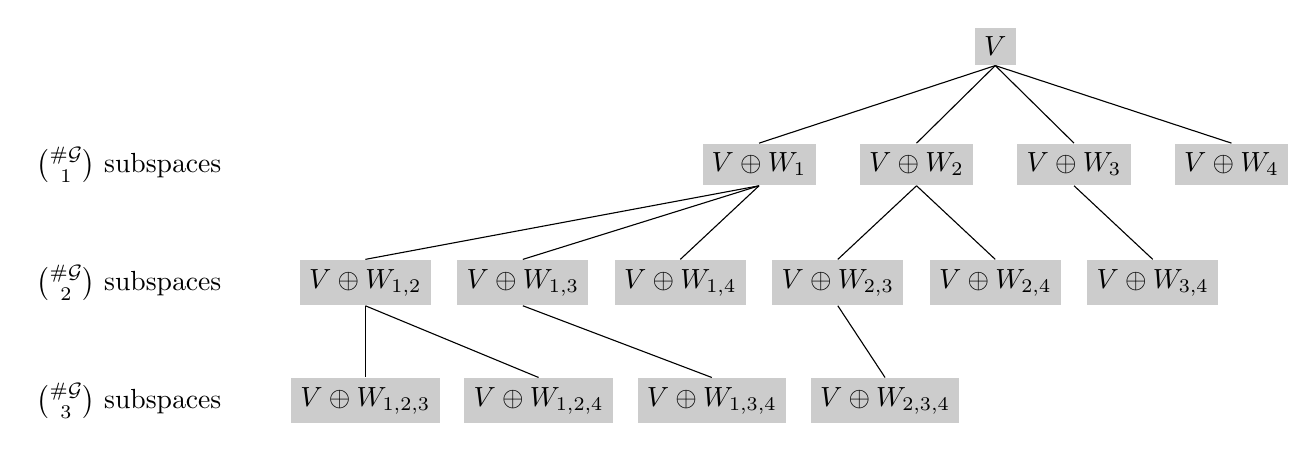
\begin{tikzpicture}
    \node[fill=black!20] (V) at (0,4.5) {$V$};
    \node[fill=black!20] (1) at (-3,3) {$V\oplus W_1$};
    \node[fill=black!20] (2) at (-1,3) {$V\oplus W_2$};
    \node[fill=black!20] (3) at (1,3) {$V\oplus W_3$};
    \node[fill=black!20] (4) at (3,3) {$V\oplus W_4$};

    \node[fill=black!20] (12) at (-8,1.5) {$V\oplus W_{1,2}$};
    \node[fill=black!20] (13) at (-6,1.5) {$V\oplus W_{1,3}$};
    \node[fill=black!20] (14) at (-4,1.5) {$V\oplus W_{1,4}$};

    \node[fill=black!20] (23) at (-2,1.5) {$V\oplus W_{2,3}$};
    \node[fill=black!20] (24) at (0,1.5) {$V\oplus W_{2,4}$};

    \node[fill=black!20] (34) at (2,1.5) {$V\oplus W_{3,4}$};

    \node[fill=black!20] (123) at (-8,0) {$V\oplus W_{1,2,3}$};
    \node[fill=black!20] (124) at (-5.8,0) {$V\oplus W_{1,2,4}$};
    \node[fill=black!20] (134) at (-3.6,0) {$V\oplus W_{1,3,4}$};
    \node[fill=black!20] (234) at (-1.4,0) {$V\oplus W_{2,3,4}$};

    \node (C1) at (-11, 3) {${\Card\G}\choose{1}$ subspaces};
    \node (C2) at (-11, 1.5) {${\Card\G}\choose{2}$ subspaces};
    \node (C3) at (-11, 0) {${\Card\G}\choose{3}$ subspaces};

    \draw (V.south) -- (1.north);
    \draw (V.south) -- (2.north);
    \draw (V.south) -- (3.north);
    \draw (V.south) -- (4.north);

    \draw (1.south) -- (12.north);
    \draw (1.south) -- (13.north);
    \draw (1.south) -- (14.north);
    \draw (2.south) -- (23.north);
    \draw (2.south) -- (24.north);
    \draw (3.south) -- (34.north);

    \draw (12.south) -- (123.north);
    \draw (12.south) -- (124.north);
    \draw (13.south) -- (134.north);
    \draw (23.south) -- (234.north);
  \end{tikzpicture}
  \caption{Tree of recursive calls in Algorithm~\ref{algo:BDEZ}, with
$\Card\G=4$ and $t-\dim V=3$.}
  \label{fig:rec-call-tree}
\end{figure}
Algorithm~\ref{algo:BDEZ} can also be adapted to find \emph{symmetric}
formulas: instead of searching in the set $\G$, we search in the set
\[
  \G_\text{sym} = \left\{ \phi\in\B\,|\,\phi\text{ is symmetric and is of rank
  }1 \right\}.
\]
Since
\[
  \Card\G_\text{sym} = \sqrt{\Card\G},
\]
the complexity of Algorithm~\ref{algo:BDEZ} adapted to the symmetric case is
naturally better.
Although not initially published in~\cite{BDEZ12}, Barbulescu, Detrey, Estibals
and Zimmerman improved on their algorithms by using symmetries in the definition
of the subspaces of $\B$. Their strategy
was described in~\cite{Covanov19}, as well as further improvements from Covanov,
exploiting even more symmetries. These ideas inspired our work on other kinds of
decompositions introduced in Chapter~\ref{chap:hypersymmetric}, for which we
provide an \emph{ad hoc} search algorithm.
% TODO: add BDEZStab (i.e. the version with RP-automorphisms)? Is that
% necessary since we do not quite use that in the case of trisymmetric bilinear
% forms? Sould we also present Covanov's method?
% 


\chapter{Hypersymmetric bilinear complexity}
\label{chap:hypersymmetric}
In Chapter~\ref{chap:bilinear}, we have seen the notions of bilinear complexity
and symmetric bilinear complexity. We now investigate even stronger
notions of symmetry, yielding to very short representations of a bilinear
map.

\minitoc

% TODO
% ====
%
% Find a nice picture to put here to illustrate something in link with the
% chapter.
%
% Note
% ====
%
% It could be an illustration of the exhaustive search tree with the rank
% technique that allows to delete some branches, a nice picture of that just
% to be ble to understand how much it deletes would be very nice imho

\clearpage
\section{Symmetric and hypersymmetric fomulas}
% Table of content
% ================
%
% - Recall of the definition of symmetric
% - Existence and lemma for the symmetric case
% - non degenerate bilinear form, link with the trace, but not only
% - Link between symmetric and hypersymmetric in smaller dimension
% - Galois invariance
% - Comment for the case of the particular algebras we study, what is known and
%   what is not
%
% Comment
% =======
%
% Comment about the trisymmetric formulas, it is true that F_4/F_2 can be
% represented by a trisymmetric formula but it is not the case for F_8/F_2. We
% should check the lemma saying something on the existence of the trisymmetric
% decomposition, but it is probably just simpler.

Let $\K$ be a finite field, $V_1$, $V_2$ and $W$ three finite-dimensional $\K$-vector
spaces and
\[
  \Phi:V_1\times V_2\to W
\]
a bilinear map. Recall Definition~\ref{defi:bilinear-formula}:
\[
  \Phi(x, y) = \sum_{j=1}^t\varphi_j(x)\psi_j(y)w_j,
\]
where for all $1\leq j\leq t$, $\varphi_j\in V_1^\vee$ and $\phi_j\in V_2^\vee$ are linear forms and
$w_j\in W$ is a vector, is called a \emph{bilinear formula} of length $t$. If
the spaces $V_1$ and $V_2$ are equal and if the bilinear map $\Phi$ is
symmetric, \ie if for all $x, y\in V$
\[
  \Phi(x, y) = \Phi(y, x),
\]
we can investigate the existence of formulas satisfying the same condition of
symmetry, \ie formulas where for all $1\leq j\leq t$, $\varphi_j=\psi_j$,
resulting in a \emph{symmetric} bilinear formula:
\[
  \Phi(x, y) = \sum_{j=1}^t\varphi_j(x)\varphi_j(y)w_j.
\]
In fact, we can define other interesting types of symmetries, but it is useful
to first generalize the notions that we saw in Chapter~\ref{chap:bilinear} to
higher dimensions.
\subsection{Generalization to multilinear maps}
The definitions of bilinear formula and bilinear complexity are not limited to the
bilinear case and can be generalized to arbitrary dimension. These general
definitions will be used in Section~\ref{subsec:trisym} to define
\emph{hypersymmetric} complexity.
\begin{defi}[Multilinear formula]
Let $V_1, V_2, \dots, V_s$ and $W$ be $s+1$ finite-dimensional $\K$-vector
spaces and
\[
  \Phi:V_1\times V_2\times\dots\times V_s\to W
\]
an $s$-linear map. A \emph{multilinear formula}, or \emph{multilinear
decomposition}, or \emph{multilinear algorithm} of length $t$ for $\Phi$ is a
collection of $s\times t$ linear forms $\varphi_1^{(1)}, \varphi_2^{(1)}, \dots,
\varphi_t^{(1)}\in V_1^\vee$ up to $\varphi_1^{(s)}, \varphi_2^{(s)}, \dots,
\varphi_t^{(s)}\in V_s^{\vee}$ and $t$ vectors $w_1, \dots, w_t$, such that for all $x_1\in V_1, \dots, x_s\in
V_s$, we have
\[
  \Phi(x_1, \dots, x_s) =
  \sum_{j=1}^t\varphi_j^{(1)}(x_1)\dots\varphi_j^{(s)}(x_s)w_j.
\]
\end{defi}
\begin{defi}[Multilinear complexity]
Let $V_1, V_2, \dots, V_s$ and $W$ be $s+1$ finite-dimensional $\K$-vector
spaces and
\[
  \Phi:V_1\times V_2\times\dots\times V_s\to W
\]
an $s$-linear map. The \emph{multilinear complexity} $\mu(\Phi)$ of $\Phi$ is the
minimal length $t$ of a multilinear formula for $\Phi$.
\end{defi}
As in the case of bilinear complexity, the multilinear complexity $\mu(\Phi)$ of a
multilinear map $\Phi$ can also be defined as the rank of the tensor in 
\[
  V_1^\vee\otimes\dots\otimes V_s^\vee\otimes W
\]
corresponding to $\Phi$, see Example~\ref{ex:bilinear-complexity} for an
illustration of this correspondence in the bilinear case. In the case where
\[
  V_1 = V_2 = \dots = V_s,
\]
symmetric formulas and
symmetric complexity can also be generalized when $\Phi$ is a \emph{symmetric}
multilinear map, \ie when for all permutations $\sigma\in\mathfrak S_s$ and for
all vectors $x_1, \dots, x_s\in V$, we have
\[
  \Phi(x_1, \dots, x_s) = \Phi(x_{\sigma(1)}, \dots, x_{\sigma(s)}).
\]
\begin{defi}[Symmetric multilinear formula]
Let $V$ and $W$ be two finite-dimensional $\K$-vector
spaces and
\[
  \Phi:\underset{\textrm{$s$ times}}{\underbrace{V\times\dots\times V}}\to W
\]
be a symmetric $s$-linear map. A \emph{symmetric multilinear formula}, or
\emph{symmetric multilinear
decomposition}, or \emph{symmetric multilinear algorithm} of length $t$ for $\Phi$ is a
collection of $t$ linear forms $\varphi_1, \varphi_2, \dots,
\varphi_t\in V^\vee$ and $t$ vectors $w_1, \dots, w_t$, such that for all $x_1, \dots, x_s\in
V$, we have
\[
  \Phi(x_1, \dots, x_s) =
  \sum_{j=1}^t\varphi_j(x_1)\dots\varphi_j(x_s)w_j.
\]
\end{defi}
\begin{defi}[Symmetric multilinear complexity]
Let $V$ and $W$ be two finite-dimensional $\K$-vector
spaces and
\[
  \Phi:\underset{\textrm{$s$ times}}{\underbrace{V\times\dots\times V}}\to W
\]
be a symmetric $s$-linear map. The \emph{symmetric multilinear complexity}
$\musym(\Phi)$ of $\Phi$ is the minimal length $t$ of a symmetric multilinear
formula for $\Phi$. If no such formula exists, we set 
\[
  \musym(\Phi) = \infty.
\]
\end{defi}
Contrary to the bilinear case, some symmetric multilinear maps do not admit a symmetric
decomposition, but the problem of whether a symmetric multilinear map admits
a symmetric multilinear formula is well understood and follows from
Theorem~\ref{thm:symmetric-formula}.
\begin{thm}[{\cite[Thm.~A.7]{Randriam15}}]\label{th:criterion}
\label{thm:symmetric-formula}
Let $\Phi:V^s\to W$ be a $s$-linear map between finite dimensional vector spaces over $\mathbb{F}_q$.
Then $\Phi$ admits a symmetric decomposition if and only if $\Phi$ is \emph{Frobenius-symmetric},
\ie if and only if it is symmetric and one of the following two conditions holds:
\begin{itemize}
\item $s\leq q$
\item $s\geq q+1$ and for all $u,v,z_1,\dots,z_{s-q-1}$ in $V$,
\[
\Phi(\underset{\textrm{$q$ times}}{\underbrace{u,\dots,u}},v,z_1,\dots,z_{s-q-1})=\Phi(u,\underset{\textrm{$q$ times}}{\underbrace{v,\dots,v}},z_1,\dots,z_{s-q-1}).
\]
\end{itemize}
\end{thm}

\subsection{Trisymmetric and hypersymmetric complexity}
\label{subsec:trisym}

Under even stricter conditions, we can study the existence of even more
symmetric formulas. These formulas allow us to describe a multilinear map with
fewer elements, and thus give a compact definition of the map. Since the
symmetry conditions are stronger there are fewer such formulas, and as a
consequence the search space is smaller. Thus, we expect search algorithms to be
faster, as was the case when using Barbulescu \etal\!\!\!'s algorithm
(Algorithm~\ref{algo:BDEZ}) to find symmetric formulas. Let us define those
``stricter conditions''. Let
\[
  \Phi:V^s\to V
\]
be an $s$-linear symmetric map, \ie we additionally ask that $W=V$. We also
assume that $V$ has a non-degenerate symmetric bilinear form, that we write as a
scalar product
\[
 \begin{array}{ccc}
 V\times V &\to&\K\\
 (v,w)&\mapsto&\ps{v}{w}.
 \end{array}
\]
In that case, we know that the vector space $V$ is isomorphic to its dual space
$V^\vee$:
\[
  V\cong V^\vee,
\]
\ie for each linear form $\varphi\in V^\vee$, there exist a unique vector $a\in
V$ such that for all $x\in V$, we have
\[
  \varphi(x) = \ps{a}{x}.
\]
Under these conditions, we can now write a symmetric formula for $\Phi$ as
\[
  \Phi(x, y) = \sum_{j=1}^t\ps{a_j}{x}\ps{a_j}{y}w_j
\]
where for all $1\leq j\leq t$, $a_j\in V$ is a vector of $V$. As a consequence,
we can also describe a symmetric formula for $\Phi$ as the data of vectors
$(a_j)_{1\leq j\leq t}$ and $(w_j)_{1\leq j\leq t}$. In order to have an even
more compact description of $\Phi$, one can ask for the vectors $w_j$ to be
proportional to $a_i$, leading to the definition of hypersymmetric
formula.
% Note
% ====
%
% But is that really natural? Wouldn't it be better to say that we would like
% the a_i and the b_i to be equal? 
%
% TODO
% ====
%
% Maybe change this to include the case a_i = b_i and discuss it a little, or
% maybe not, we'll see.
%
% Remark
% ======
%
% If this is presented, it could be nice to have the tensor point of view, with
% a decomposition with the same elements three times being then very clear.

\begin{defi}[Hypersymmetric formula]
Let $V$ be a finite-dimensional $\K$-vector
space equipped with a scalar product and
\[
  \Phi:\underset{\textrm{$s$ times}}{\underbrace{V\times\dots\times V}}\to V
\]
a symmetric $s$-linear map. A \emph{hypersymmetric formula}, or
\emph{hypersymmetric decomposition}, or \emph{hypersymmetric algorithm} of length $t$ for $\Phi$ is a
collection of $t$ vectors $a_1, \dots, a_t\in V$ and $t$ scalars $\lambda_1,
\dots, \lambda_t\in\K$, such that for all $x_1, \dots, x_s\in
V$, we have
\[
  \Phi(x_1, \dots, x_s) =
  \sum_{j=1}^t\lambda_j\ps{a_j}{x_1}\dots\ps{a_j}{x_s}a_j.
\]
\end{defi}
\begin{defi}[Hypersymmetric complexity]
Let $V$ be a finite-dimensional $\K$-vector space equipped with a scalar product
and
\[
  \Phi:\underset{\textrm{$s$ times}}{\underbrace{V\times\dots\times V}}\to V
\]
a symmetric $s$-linear map. The \emph{hypersymmetric complexity} $\muhyp(\Phi)$ of $\Phi$ is the
minimal length $t$ of a hypersymmetric formula for $\Phi$. If no such
formula exists, we set
\[
  \muhyp(\Phi) = \infty.
\]
\end{defi}
\begin{ex}
  \label{ex:trisymmetric-formula}
  We take the same case as in Example~\ref{ex:bilinear-complexity}, but viewed
  a bit differently. Let $\K=\mathbb{F}_2$ and 
  \[
    V=\mathbb{F}_4\cong\mathbb{F}_2[T]/(T^2+T+1)\cong\mathbb{F}_2(\zeta)
  \]
  seen as a $\mathbb{F}_2$-vector space of dimension $2$ using the base $(1,
  \zeta)$. The $\mathbb{F}_2$-bilinear map $\Phi$ that we
  consider is the product in $\mathbb{F}_4$:
  \[
 \begin{array}{cccc}
   \Phi: & \mathbb{F}_4\times \mathbb{F}_4 &\to&\mathbb{F}_4\\
 &(x,y)&\mapsto&xy.
 \end{array}
  \]
  We also consider the non-degenerate symmetric bilinear form
\[
 \begin{array}{ccc}
   \mathbb{F}_4\times \mathbb{F}_4 &\to&\mathbb{F}_2\\
 (v,w)&\mapsto&\tr(vw),
 \end{array}
\]
where $\tr$ is the trace of the field extension $\mathbb{F}_4/\mathbb{F}_2$,
and we write
\[
  \tr(xy) = \ps{x}{y}.
\]
If $x = x_0 + x_1\zeta\in\mathbb{F}_4$ is an element in the extension field, we have $\tr(x) = x_1$, and if $y = y_0
+ y_1\zeta\in\mathbb{F}_4$ is another element, then their product is
\[
  xy = x_0y_0 + x_1y_1 + (x_0y_1 + x_1y_0 + x_1y_1)\zeta.
\]
We also see that
\[
\left\{ 
  \begin{array}{lll}
    \ps{1}{x}\ps{1}{y} &=& x_1y_1 \\
    \ps{1+\zeta}{x}\ps{1+\zeta}{y} &=& x_0y_0 \\
    \ps{\zeta}{x}\ps{\zeta}{y} &=& (x_0+x_1)(y_0+y_1)
  \end{array}
\right.
\]
and thus we have
\[
  xy =
  \ps{1}{x}\ps{1}{y}\cdot1+\ps{1+\zeta}{x}\ps{1+\zeta}{y}\cdot(1+\zeta)+\ps{\zeta}{x}\ps{\zeta}{y}\cdot\zeta.
\]
This is an hypersymmetric formula of length $3$, and we can prove that there are
no formulas of length $2$, so we have
\[
  \muhyp(\Phi) = 3.
\]
This is in fact the very same formula as in
Example~\ref{ex:bilinear-complexity}.
\end{ex}
In order to investigate the existence of hypersymmetric decompositions, we
remark that there is a natural link between hypersymmetric decompositions of 
the $s$-linear map
\[
  \Phi:V^s\to V
\]
and symmetric decompositions of the $(s+1)$-linear form $\widetilde\Phi$ defined by
\[
  \begin{array}{llll}
    \widetilde\Phi:&V^{s+1}&\to&\K\\
    &(x_1, \dots, x_{s+1})&\mapsto&\ps{\Phi(x_1, \dots, x_s)}{x_{s+1}}
  \end{array}
\]
given by Lemma~\ref{lm:link-hyp-sym}.
Definition~\ref{defi:hypersymmetric-map} follows from this correspondence.
\begin{lm}
  \label{lm:link-hyp-sym}
  Let $V$ a $\K$-vector space and 
  \[
    \Phi:V^s\to V
  \]
  a symmetric $s$-linear map. 
Elements $(a_j)_{1\leq j\leq t}$ in $V$ and scalars $(\lambda_j)_{1\leq j\leq
t}$ in $\K$ define a hypersymmetric formula for the $s$-linear map $\Phi$,
\[
\Phi(x_1,\dots,x_s)=\sum_{j=1}^{t}\lambda_j\ps{a_j}{x_1}\cdots\ps{a_j}{x_s}a_j,
\]
if and only if they define a symmetric formula for the $(s+1)$-linear form $\widetilde{\Phi}$,
\[
\widetilde{\Phi}(x_1,\dots,x_s,x_{s+1})=\sum_{j=1}^{t}\lambda_i\ps{a_j}{x_1}\cdots\ps{a_j}{x_s}\ps{a_j}{x_{s+1}}.
\]

Thus, $\Phi$ admits a hypersymmetric formula if and only if $\widetilde{\Phi}$ is Frobenius-symmetric (in the sense of Theorem~\ref{thm:symmetric-formula}),
and we have
\[
\muhyp(\Phi)=\musym\left(\widetilde{\Phi}\right).
\]

In particular, if $q\geq s+1$, then any hypersymmetric $s$-linear map over $\mathbb{F}_q$ admits a hypersymmetric formula.
\end{lm}
\begin{proof}
  Assume that $\Phi$ admits a hypersymmetric decomposition, such that for all
  $x_1, \dots, x_s\in V$, we have
  \[
    \Phi(x_1,\dots,x_s)=\sum_{j=1}^{t}\lambda_i\ps{a_j}{x_1}\cdots\ps{a_j}{x_t}a_j,
  \]
  then, by taking the scalar product with any $x_{s+1}$, we obtain
\[
  \ps{\Phi(x_1, \dots,
  x_s)}{x_{s+1}}=\widetilde{\Phi}(x_1,\dots,x_s,x_{s+1})=\sum_{j=1}^{t}\lambda_i\ps{a_j}{x_1}\cdots\ps{a_j}{x_s}\ps{a_j}{x_{s+1}},
\]
which defines a symmetric decomposition for $\widetilde\Phi$. In the other
direction, assume that $\widetilde\Phi$ admits a symmetric decomposition, such
that for all $x_1, \dots, x_{s+1}\in V$, we have
\[
\widetilde{\Phi}(x_1,\dots,x_s,x_{s+1})=\sum_{j=1}^{t}\lambda_i\ps{a_j}{x_1}\cdots\ps{a_j}{x_s}\ps{a_j}{x_{s+1}}.
\]
It can also be written as
\[
  \ps{\Phi(x_1, \dots,
  x_s)}{x_{s+1}}=\ps{\sum_{j=1}^t\lambda_j\ps{a_j}{x_1}\cdots\ps{a_j}{x_s}a_j}{x_{s+1}},
\]
so that we have
\[
  \ps{\Phi(x_1, \dots,
  x_s)-\sum_{j=1}^t\lambda_j\ps{a_j}{x_1}\cdots\ps{a_j}{x_s}}{x_{s+1}}=0.
\]
Since the scalar product $\ps{\cdot}{\cdot}$ is non-degenerate, it means that
  \[
    \Phi(x_1,\dots,x_s)=\sum_{j=1}^{t}\lambda_i\ps{a_j}{x_1}\cdots\ps{a_j}{x_t}a_j.
  \]
  Hence $\Phi$ admits a hypersymmetric decomposition. The other assertions
  follow.
\end{proof}
\begin{defi}[Hypersymmetric map]
  \label{defi:hypersymmetric-map}
  An $s$-linear map 
  \[
    \Phi:V^s\to V
  \]
  is called \emph{hypersymmetric} if the associated $(s+1)$-linear
  form $\widetilde\Phi$ is symmetric.
\end{defi}

The most important case is arguably the bilinear case, where $s=2$, because it
was thoroughly studied. For that reason, we sometimes replace the word
hypersymmetric by \emph{trisymmetric} in that particular case, because of the
form of the formulas
\[
  \Phi(x, y) = \sum_{j=1}^t\lambda_j\ps{a_j}{x}\ps{a_j}{y}a_j
\]
that includes the same element $a_j$ three times, and we write $\mutri(\Phi)$
instead of $\muhyp(\Phi)$. Lemma~\ref{lm:link-hyp-sym} states that, if $q\geq3$, a
trisymmetric map $\Phi$ always admits a trisymmetric decomposition.

\subsection{Galois invariance}

Another type of interesting decompositions is Galois invariant decompositions,
that we also call $\sigma$-invariant decompositions.
It is motivated by the study of group actions on the set of decompositions, that
can sometimes be used to cut branches in the search tree of the algorithms.
% TODO
% ====
%
% Link that with BDEZ stab, the version using automorphisms, and Covanov.
Let 
\[
 \begin{array}{cccc}
   \sigma: & V &\to&V\\
 &x&\mapsto&x^\sigma
 \end{array}
\]
be a $\K$-automorphism of $V$ that respects the scalar product, \ie for all $x,
y\in V$, we have
\[
  \ps{x^\sigma}{y^\sigma} = \ps{x}{y}.
\]
Then, if $\sigma$ is also compatible with some multilinear map $\Phi$, it induces
an action on the set of decompositions, as explained in
Lemma~\ref{lm:action-sym}.
\begin{lm}
  \label{lm:action-sym}
  Let $V$ be a finite-dimensional $\K$-vector space and
  \[
    \Phi:V^s\to V
  \]
  be a symmetric $s$-linear map that is compatible with $\sigma$, \ie for all
  $x_1, \dots, x_s$ in $V$, we have
  \[
    \Phi(x_1^\sigma, \dots, x_s^\sigma) = \Phi(x_1, \dots, x_s)^\sigma.
  \]
  If $(a_j)_{1\leq j \leq t}$ and $(b_j)_{1\leq j \leq t}$ define a symmetric
  formula for $\Phi$
  \[
    \Phi(x_1, \dots, x_s) = \sum_{j=1}^t\ps{a_j}{x_1}\dots\ps{a_j}{x_s}b_j,
  \]
  then $(a_j^\sigma)_{1\leq j\leq t}$ and $(b_{j}^\sigma)_{1\leq j\leq t})$ also
  define a symmetric formula for $\Phi$
  \[
    \Phi(x_1, \dots, x_s) =
    \sum_{j=1}^t\ps{a_j^\sigma}{x_1}\dots\ps{a_j^\sigma}{x_s}b_j^\sigma.
  \]
\end{lm}
\begin{proof}
 Assume that we have a symmetric decomposition for $\Phi$, with the same
 notations as in the Lemma. First, notice that for every $x,y\in V$, we have
 \[
   \ps{x^\sigma}{y} = \langle{x},{y^{\sigma^{-1}}}\rangle.
 \]
 Then, it follows that
 \begin{align*}
   \Phi(x_1, \dots, x_s) &= \Phi(x_1^{\sigma^{-1}}, \dots,
   x_{s}^{\sigma^{-1}})^\sigma\\
   &=
   (\sum_{j=1}^t\langle{a_j},{x_1^{\sigma^{-1}}}\rangle\dots\langle{a_j},{x_s^{\sigma^{-1}}}\rangle
   b_j)^\sigma\\
   &= \sum_{j=1}^t\ps{a_j^{\sigma}}{x_1}\dots\ps{a_j^\sigma}{x_s}b_j^\sigma.
 \end{align*}
 Thus we have a new symmetric formula for $\Phi$.
\end{proof}
When this action, does not change the formula, we then say that it is
$\sigma$-invariant.
\begin{defi}[$\sigma$-invariance]
  Let $(a_j)_{1\leq j\leq t}$ and
$(b_j)_{1\leq j\leq t}$ define a symmetric formula for $\Phi$
  \[
    \Phi(x_1, \dots, x_s) = \sum_{j=1}^t\ps{a_j}{x_1}\dots\ps{a_j}{x_s}b_j.
  \]
We say that this
formula is $\sigma$-invariant if it is the same as the formula defined by
$(a_j^\sigma)_{1\leq j\leq t}$ and $(b_j^\sigma)_{1\leq j\leq t}$,
\ie if there is a permutation $\pi\in\mathfrak S_t$ of $\{1,\dots,t\}$ such that
$(a_j^\sigma,b_j^\sigma)=(a_{\pi(j)},b_{\pi(j)})$ for all $j$. This also applies
to hypersymmetric formulas, setting $b_j=\lambda_j a_j$. 
\end{defi}
\begin{ex}
  In fact, the trisymmetric formula seen in
  Example~\ref{ex:trisymmetric-formula} was already $\sigma$-invariant. Recall
  that we work in $\mathbb{F}_4$, defined by
  \[
   \mathbb{F}_4\cong\mathbb{F}_2[T]/(T^2+T+1)\cong\mathbb{F}_2(\zeta),
  \]
  and we take
\[
  \tr(xy) = \ps{x}{y}.
\]
The $\mathbb{F}_2$-automorphism that we consider is the Frobenius automorphism
\[
  \begin{array}{cccc}
    \sigma: & \mathbb{F}_4 & \to & \mathbb{F}_4 \\
    & x & \mapsto & x^2.
  \end{array}
\]
We still have, for all $x, y\in\mathbb{F}_4$
\[
  xy =
  \ps{1}{x}\ps{1}{y}\cdot1+\ps{1+\zeta}{x}\ps{1+\zeta}{y}\cdot(1+\zeta)+\ps{\zeta}{x}\ps{\zeta}{y}\cdot\zeta.
\]
Since
\[
\left\{ 
  \begin{array}{l}
    1^\sigma = 1 \\
    \zeta^\sigma=\zeta+1\\
    (\zeta+1)^\sigma=\zeta
  \end{array}
\right.
\]
we see that the formula is $\sigma$-invariant.
\end{ex}

\subsection{Multiplication formulas in algebras}
\label{sec:formulas-algebras}

In the previous pages, we defined (hyper)symmetric formulas for any
multilinear map defined over some finite-dimensional $\K$-vector space.
Nevertheless, as seen in the examples, we are often interested in special
instances of multilinear maps. In fact, the map that we have in mind is almost
always the binary product of some $\K$-algebra $\A$. There are
two types of algebras we are particularly interested in.
\begin{itemize}
  \item The finite field extensions $\A=\mathbb{F}_{q^k}$, in which we take the
    trace bilinear form
    \[
      \ps{x}{y}=\tr(xy)
    \]
    for our scalar product, and the Frobenius automorphism
    \[
  \begin{array}{cccc}
    \sigma: & \mathbb{F}_{q^k} & \to & \mathbb{F}_{q^k} \\
    & x & \mapsto & x^q.
  \end{array}
\]
for our $\K$-automorphism.
\item Algebras of truncated polynomials $\A = \mathbb{F}_q[T]/(T^k)$. In this
  case, we let 
  \[
  \begin{array}{cccc}
    \tau: & \A & \to & \K \\
    & \sum_{j=0}^{k-1}x_j T^j & \mapsto & x_0
  \end{array}
\]
and
\[
  \ps{x}{y} = \tau(xy).
\]
Indeed, if $x=\sum_{j=0}^{k-1}T^j$ and $y=\sum_{j=0}^{k-1}y_jT^j$, we have
\[
  \tau(x, y) = x_0y_{k-1} + x_1y_{k-2} + \dots + x_{k-1}y_0,
\]
thus $\tau$ is a non-degenerate bilinear form.
\end{itemize}
We denote by $\mutri_q(k)$ the trisymmetric bilinear complexity of the
$2$-variable product in $\mathbb{F}_{q^k}$ and by $\hmutri_q(k)$ the
trisymmetric bilinear complexity of the $2$-variable product in
$\mathbb{F}_q[T]/(T^k)$.

\section{Algorithmic search in small dimension}

In very small dimension, \eg in Examples~\ref{ex:bilinear-complexity}
and~\ref{ex:trisymmetric-formula} where we are working with $\K$-vector spaces
of dimension $2$, the search for formulas can be done by hand relatively easily
because the length of the formulas is short. Though, even in small dimension, if
the size of $\K$ is large, the number of different formulas can be
big, thus making it hard to list \emph{all} different solutions. For these
reasons, it is highly desirable to \emph{algorithmically} find the formulas.
Let $V$ be a finite dimensional $\K$-vector space and $\Phi:V\times V\to V$ a bilinear map.
When wanting to list all the symmetric formulas of the form
\[
  \Phi(x, y) = \sum_{j=0}^t\varphi_j(x)\varphi_j(y)a_j,
\]
Barbulescu~\etal\!\!\!'s and Covanov's algorithms exhaustively search through
all linear forms $\varphi$, cleverly eliminating useless branches in the search
tree. Nevertheless, their methods exploit the fact that it is possible to freely
choose the vectors $a_j\in V$, independently of the linear forms $\varphi_j\in
V^\vee$. This is
no longer possible when searching for trisymmetric decompositions
\[
  \Phi(x, y) = \sum_{j=0}^t\lambda_j\ps{a_j}{x}\ps{a_j}{y}a_j,
\]
because each
linear form $\varphi\in V^\vee$ is linked with a unique vector $a\in V$ such
that for all $x\in V$
\[
  \varphi(x) = \ps{a}{x},
\]
and the choice of a linear form $\varphi_j$ with $\varphi_j(x)=\ps{a_j}{x}$
imposes the choice of the vector $a_j\in V$. We thus propose an \emph{ad hoc}
algorithm to find trisymmetric formulas, exploiting the vector space structure.

\subsection{General algorithm description}
\label{sec:general-algorithm}

In all the section, we assume that $\K=\mathbb{F}_q$ is the finite field with
$q$ elements, $V$ is a finite-dimensional $\K$-vector space equipped with a
non-degenerate bilinear form, written as a saclar product $\ps{\cdot}{\cdot}$,
and $\Phi:V\times V\to V$ is a hypersymmetric bilinear map for which we want to
compute trisymmetric decompositions
\[
  \Phi(x, y) = \sum_{j=1}^t\lambda_j\ps{a_j}{x}\ps{a_j}{y}a_j.
\]
Assume that
\[
  V\cong\K^k
\]
is a $\K$-vector space of dimension $k$, for which a basis has been chosen and
allows us to identify $V$ to $\K^k$, and
let $(b_j)_{1\leq j\leq k}$ be the projections of $\Phi$ on each coordinate, \ie for
all $x,y\in V$, we have
\[
  \Phi(x, y) = (b_1(x, y), \dots, b_k(x, y)).
\]
We already saw that the difficulty in the trisymmetric case resides in the
fact that each linear form, or equivalently each symmetric rank $1$ bilinear
form, comes with a given vector in $V$ that dictates its impact on the different
coordinates in a trisymmetric formula. Therefore, a central idea is to
exhaustively search through vectors in $V$ instead of linear forms in $V^\vee$.
This is equivalent since 
\[
  V\cong V^\vee
\]
in this case anyway. Moreover, we search through special sets of vectors that
have easy-to-manage coordinates, \eg well-placed zeros and ones, in order to
control the impact on certain coordinates. Assume $(a_j)_{1\leq j \leq t}$ in $V$ and
$(\lambda_j)_{1\leq j \leq t}$ in $\K$ define a trisymmetric decomposition
\[
  \Phi(x, y) = \sum_{j=1}^t\lambda_j\ps{a_j}{x}\ps{a_j}{y}a_j.
\]
Without loss of generality, we can consider that every element $a_j$ is
``normalized'', \ie its first nonzero coordinate is $1$. Indeed, if we have one
\[
  a_{j_0} = 0
\]
for some $1\leq j_0 \leq t$, then we just remove one term from the formula and
we still have a trisymmetric decomposition, of length $t-1$. Now if for every
$1\leq j\leq t$, 
\[
  a_j\neq0,
\]
we let $x_j$ be the first nonzero coordinate of $a_j$ and we write
\[
  a_j = x_j \widetilde a_j.
\]
We can now write the trisymmetric formula as
\begin{align*}
  \Phi(x, y) &= \sum_{j=1}^t\lambda_j\ps{a_j}{x}\ps{a_j}{y}a_j \\
  &= \sum_{j=1}^t\lambda_j\ps{x_j\widetilde a_j}{x}\ps{x_j\widetilde
  a_j}{y}x_j\widetilde a_j \\
  &= \sum_{j=1}^t\lambda_jx_j^3\ps{\widetilde a_j}{x}\ps{\widetilde
  a_j}{y}\widetilde a_j \\
  &= \sum_{j=1}^t\widetilde \lambda_j\ps{\widetilde a_j}{x}\ps{\widetilde
  a_j}{y}\widetilde a_j,
\end{align*}
where $\widetilde\lambda_j = \lambda_jx_j^3$.
Therefore any trisymmetric formula is equivalent to a trisymmetric formula with
normalized vectors, and thus we only search for formulas with normalized
elements. In other words, for all $1\leq i\leq k$, we let
\[
  \E_i=\left\{ x=(x_1, \dots, x_k)\in V
  \,|\, \forall l\leq i-1,\,x_l=0\text{ and }x_i=1 \right\}
\]
and
\[
  \E = \bigcup_{i=1}^k\E_i,
\]
and we search for elements $a_j$ in $\E$ instead of the entire vector space $V$.
Limiting the search to $\E$ helps us in two different ways. First, it reduces
the complexity of the exhaustive search since the size of $\E$ is smaller
than the size of $V$. Indeed, the sets $\E_i$ are disjoint, so
\begin{align*}
  \Card\E &= \sum_{i=1}^k\Card\E_i\\
  &= \sum_{i=1}^k q^{k-i}\\
  &= \cfrac{q^k-1}{q-1},
\end{align*}
whereas
\[
  \Card V = q^k.
\]
Second, it leads to a better understanding of what happens in the algorithm,
because if we have some vector
\[
  a\in\E_i
\]
for a given $1\leq i\leq k$, we know that the associated bilinear form
\[
  (x, y)\mapsto\ps{a}{x}\ps{a}{y}
\]
can only impact the coordinates $l\geq i$. Thus, we further
use the vector space structure of $V$ by searching for solutions
on each coordinate, starting with the first coordinates and vectors in $\E_1$,
then the second coordinate and vectors in $\E_2$, and so on until the last
coordinate. Let us focus on the first coordinate and give some details.

Recall that the goal is to obtain a trisymmetric decomposition for the
hypersymmetric bilinear map $\Phi:V\times V\to V$, that is written
\[
  \Phi(x, y) = (b_1(x, y), \dots, b_k(x, y)).
\]
in the basis of $V$. We first see how to decompose the bilinear \emph{form}
$b_1$ as a sum of rank $1$ bilinear forms. Let $\B$ be the set of bilinear forms
of $V\times V$, recall that $\B$ is a $\K$-vector space of dimension $k^2$, and
that we identify $b_1$ with the $k\times k$ matrix $B_1\in\K^{k\times k}$ 
such that for all vectors $x, y\in V$, we have
\[
  b_1(x, y) = X B_1 Y^t,
\]
where $X, Y\in\K^{1\times k}$ are the row vectors representing $x$ and $y$ and
where $Y^t$ is the transpose of $y$. Let $r_1$ be the rank of $b_1$, we know
that $b_1$ can be decomposed as a sum of $r_1$ bilinear forms of rank $1$. Let
$f$ be the application mapping an element in $V$ to its associated bilinear
form:
\[
  \begin{array}{cccc}
    f: & V & \to & \B\\
    & a & \mapsto & (x, y)\mapsto\ps{a}{x}\ps{a}{y}.
  \end{array}
\]
In order to find these decompositions, we begin by exhaustively searching through scalars $\lambda_1\in\K$ and vectors
$a_1\in \E_1$ such that
\[
  r_1-1=\rank(b_1-\lambda_1 f(a_1)) < \rank(b_1)=r_1.
\]
Then, for each such pair $(\lambda_1, a_1)$, we exhaustively search through
scalars $\lambda_2\in\K$ and vectors $a_2\in \E_1$ such that
\[
  r_1-2=\rank(b_1-\lambda_1 f(a_1)-\lambda_2f(a_2)) < \rank(b_1-\lambda_1
  f(a_1))=r_1-1.
\]
We continue this process until we have $r_1$ pairs $(\lambda_1, a_1), \dots,
(\lambda_{r_1}, a_{r_1})$ such that
\[
  0 = \rank(b_1-\sum_{j=1}^{r_1}\lambda_jf(a_j)) <
  \rank(\sum_{j=1}^{r_1-1}\lambda_jf(a_j)) = 1,
\]
which exactly means that
\[
  b_1 = \sum_{j=1}^{r_1}\lambda_jf(a_j),
\]
and we have found our decomposition.
In fact, we can search in a more clever way. Since the rank of $b_1$ is $r_1$
and we are looking for decompositions as a sum of exactly $r_1$ bilinear forms of
rank $1$, we must choose
pairs $(\lambda_j, a_j)$ that decrease the rank of our bilinear form at each
step, otherwise we will need strictly more than $r_1$ bilinear forms of rank
$1$. Therefore, at each step, we can search only through the vectors that can
decrease the rank of the last considered bilinear form. After each choice of
$(\lambda_1, a_1)$, we will thus exhaustively search through scalars
$\lambda_2\in\K$ and vectors $a_2$ in
\[
  \E_1^{\left\{ (\lambda_1, a_1) \right\}} = \left\{
    a\in\E_1\mid\text{there exists}\,\lambda\in\K\text{ such that}\,\rank(b_1-\lambda f(a)) <\rank(b_1)
\right\}.
\]
Then, after each choice of $(\lambda_2, a_2)$, we will search through scalars
$\lambda_3\in\K$ and vectors $a_3$ in
\[
  \E_1^{\left\{ (\lambda_1, a_1), (\lambda_2, a_2) \right\}} = \left\{
    a\in\E_1^{ \left\{ (\lambda_1, a_1)
    \right\}}\;|\;\exists\lambda\in\K,\,\rank(b_1-\lambda_1f(a_1)-\lambda f(a))
    <\rank(b_1-\lambda_1f(a_1))
\right\},
\]
and we use the same idea until the end of the process. This strategy, used in
Algorithm~\ref{algo:mindecomp}, 
saves a lot of time in the search because we look only at the vectors that have
the potential to decrease the rank, instead of all the vectors in $\E_1$.
\begin{algorithm}
  \caption{(Minimal decomposition)}
  \label{algo:mindecomp}
  \begin{algorithmic}[1]
    \Require{$b\in \B$ a bilinear form of rank $r$, $E\subset\E$
    the space of vectors where to search}
    \Ensure{A list of decompositions of $b$ as a sum of bilinear forms of rank
    $1$, each decomposition represented by a set of $r$ pairs $\left\{
      (\lambda_1, a_1), \dots, (\lambda_{r}, a_{r})\right\}$.}

    \Procedure{MinimalDecomposition}{$b, E, R_{\text{glob}},
    R_{\text{loc}}=\emptyset$}
    \If{$\varphi=0$}\Comment{$\rank(\varphi)=0$}
    \State $R_\text{glob}\gets R_\text{glob}\bigcup\left\{R_\text{loc}\right\}$
    \Else
    \State $\mathcal C\gets\emptyset$\Comment{$\mathcal C$ is the set of pairs
    that decrease the rank}
    \ForAll{$a\in E$}
    \ForAll{$\lambda\in\K$}
  \If{$\rank(b-\lambda f(a))<\rank(b)$}
    \State $\mathcal C\gets\mathcal C\bigcup\left\{ (\lambda, a) \right\}$
    \State \textbf{break}\Comment{breaks only the inner loop}
    \EndIf
    \EndFor
    \EndFor
    \For{$i=1$ to $\Card\mathcal C$}\Comment{we note $\mathcal
      C=\left\{ (\gamma_1, c_1), \dots, (\gamma_u, c_u) \right\}$}
      \State $E'\gets\left\{ c_{i+1}, \dots, c_u \right\}$
    \State \Call{MinimalDecomposition}{$b-\gamma_i f(c_i), E', R_\text{glob},
    R_\text{loc}\cup\left\{ (\gamma_i, c_i) \right\}$}
    \EndFor
    \EndIf
    \EndProcedure

   \State $\mathcal R\gets\emptyset$
    \State \Call{MinimalDecomposition}{$b, E, \mathcal R$}
    \State \Return $\mathcal R$
  \end{algorithmic}
\end{algorithm}


For each decomposition of $b_1$
\[
  b_1(x, y) = \sum_{j=1}^{r_1}\lambda_j\ps{a_j}{x}\ps{a_j}{y}
\]
that we compute this way, we obtain
\[
  \Phi(x, y) - \sum_{j=1}^{r_1}\lambda_j\ps{a_j}{x}\ps{a_j}{y}a_j = (0, b_2'(x,
  y), \dots, b_k'(x, y)),
\]
where $b_2', \dots, b_k'\in\B$ are new bilinear forms, depending on the coordinates
of $a_1, \dots, a_{r_1}$, and where the first coordinate is $0$ because the
first coordinate of the vectors $a_1, \dots, a_{r_1}$ is always $1$. Then, we
use Algorithm~\ref{algo:mindecomp} with the bilinear form $b_2'$ of rank $r_2$ and the initial
set of vectors $\E_2$. For each decomposition of $b_2'$
\[
  b_2'(x, y) = \sum_{j=r_{1}+1}^{r_1+r_2}\lambda_j\ps{a_j}{x}\ps{a_j}{y}
\]
obtained, we have
\[
  \Phi(x, y) - \sum_{j=1}^{r_1+r_2}\lambda_j\ps{a_j}{x}\ps{a_j}{y}a_j = (0, 0,
  b_3''(x, y), \dots, b_k''(x, y)),
\]
where $b_3'', \dots, b_k''\in\B$ are again new bilinear forms, depending on the
coordinates of the elements $a_{r_1+1}, \dots, a_{r_1+r_2}$. We continue this
process on all the coordinates, such that in the end we obtain trisymmetric
decompositions of the form
\[
  \Phi(x, y) = \sum_{j=1}^t\lambda_j\ps{a_j}{x}\ps{a_j}{y}a_j.
\]
The overall strategy is described in Algorithm~\ref{algo:trisymmin}.
\begin{algorithm}
  \caption{(Trisymmetric search with minimal
  decompositions)}\label{algo:trisymmin}
  \begin{algorithmic}[1]
    \Require{$\Phi=(b_1, \dots, b_k)$ a bilinear map;
      $t\in\mathbb{N}$ an integer}
    \Ensure{A list of trisymmetric decompositions of $\Phi$ of length up to $t$.}

    \Procedure{TriSymSearchMin}{$\Phi, t, S_\text{glob}, i=1,
    S_\text{loc}=\emptyset$}
      \If{$\Phi = 0$}
      \State $S_\text{glob}\gets S_\text{glob}\bigcup \left\{S_\text{loc}\right\}$.
      \ElsIf{$\rank(b_i)\leq t$}
        \State $\mathcal R\gets\emptyset$
        \State \Call{MinimalDecomposition}{$b_i, \E_i,
        \mathcal R$}\Comment{We have $\Phi=(b_1, \dots, b_k)$}
        \ForAll{$S\in\mathcal R$}
        \State $\Phi'\gets\Phi-\sum_{(\lambda, \alpha)\in
        S}\lambda\f(\alpha)\alpha$
        \State \Call{TriSymSearchMin}{$\Phi', t-\Card S, S_\text{glob}, i+1,
          S_\text{loc}\cup S$}
        \EndFor
      \EndIf
    \EndProcedure
    \State $\mathcal S\gets\emptyset$
    \State \Call{TriSymSearchMin}{$\Phi, t, \mathcal S$}
    \State \Return $\mathcal S$
  \end{algorithmic}
\end{algorithm}

Let $(\lambda_j)_{1\leq j\leq t}$ be some scalars in $\K$ and $(a_j)_{1\leq
j\leq t}$ some vectors in
\[
  \E=\bigcup_{i=1}^k\E_i
\]
that define an optimal trisymmetric decomposition for $\Phi$
(\ie the length of the decomposition is minimal): 
\[
  \Phi(x, y) = \sum_{j=1}^t\lambda_j\ps{a_j}{x}\ps{a_j}{y}a_j.
\]
Although the formula is optimal, it is entirely possible for the individual
coordinate decompositions to be sub-optimal. Assume that for all vectors $x,
y\in V$, we have
\[
  \Phi(x, y) = (b_1(x, y), \dots, b_k(x, y)),
\]
with $r_1$ the rank of the bilinear form $b_1\in\B$. If we have strictly more
than $r_1$ different vectors in $(a_j)_{1\leq j\leq t}$ that belong to $\E_1$,
then Algorithm~\ref{algo:trisymmin} will not find this decomposition. Indeed,
Algorithm~\ref{algo:mindecomp} only finds \emph{minimal} decompositions of $b_1$
into $r_1$ bilinear forms of rank $1$, \ie finds decompositions with exaclty
$r_1$ vectors in $(a_j)_{1\leq j\leq t}$ that are in $\E_1$. More generally, in
Algorithm~\ref{algo:mindecomp}, when working with a bilinear form $b$ of rank
$r$, it is possible that the best \emph{local} decompositions (\ie on only one
coordinate) of length $r$ are not the best in order to find \emph{global}
decompositions (\ie on all the coordinates), because of the impact the
decompositions of $b$ have on the other coordinates. For that reason, it is
important to add the option in Algorithm~\ref{algo:mindecomp} to search for
non-optimal decompositions. That is exactly what is done in
Algorithm~\ref{algo:decompmargin}: if we want to find all decompositions of some
bilinear form $b$ of rank $r$ of length $r+\mu$, with $\mu>0$, we still
exhaustively search through scalars $\lambda\in\K$ and vectors $a\in\E$, but we
allow the rank \emph{not to} decrease on $\mu$ different times. Once this number
of ``exceptions'' have all been used, we go back to the strategy previously
presented (\ie Algorithm~\ref{algo:mindecomp}).
% TODO:
% ====
%
% As written by Luca, what is the link between this ad hoc algorithm and the
% ones that we could use for obtaining symmetric decompositions of the symmetric
% *form* in dimension s+1 corresponding to the map, cf Lemma 4.1.9

\begin{algorithm}
  \caption{(Decomposition with margin)}\label{algo:decompmargin}
  \begin{algorithmic}[1]
    \Require{$b\in \B$ a bilinear form of rank $r$, $E\subset\E$
    the space of vectors in which to search, $\mu$ the margin, $t$ the maximum
  length of a decompositon of $b$}
    \Ensure{A list of decompositions of $b$ as a sum of at bilinear forms of rank
    $1$, each decomposition represented by a set of at most $t$ pairs $\left\{
      (\lambda_1, a_1), \dots, (\lambda_{t}, a_{t})\right\}$.}

    \Procedure{DecompositionWithMargin}{$b, E, r, \mu, R_{\text{glob}},
    R_{\text{loc}}=\emptyset$}
    \If{$\rank b\leq t$}
    \If{$b=0$}\Comment{$\rank b=0$}
    \State $R_\text{glob}\gets R_\text{glob}\bigcup\left\{R_\text{loc}\right\}$
    \ElsIf{$\mu=0$}\Comment{No margin left!}
    \State \Call{MinimalDecomposition}{$\varphi, E, R_\text{glob},
    R_\text{loc}$}\Comment{"naive" strategy: Alg.~\ref{algo:mindecomp}}
   \Else
   \For{$i=1$ to $\Card E$}\Comment{We note $E=\left\{ c_1, \dots, c_u \right\}$}
   \State $E'\gets\left\{ c_{i+1}, \dots, c_u \right\}$
    \ForAll{$\lambda\in\mathbb{F}_p$}
    \State $b'\gets b-\lambda f(c_i)$
    \State $R_\text{loc}'\gets R_\text{loc}\bigcup\left\{ (\lambda, c_i)
    \right\}$
    \If{$\rank(b')<\rank(b)$}
    \State \Call{DecompositionWithMargin}{$b', E', t-1, \mu,
      R_\text{glob}, R_\text{loc}'$}
    \Else
    \State \Call{DecompositionWithMargin}{$b', E', t-1, \mu-1,
      R_\text{glob}, R_\text{loc}'$}
    \EndIf
    \EndFor
    \EndFor
    \EndIf
    \EndIf
    \EndProcedure

    \State $\mathcal R\gets\emptyset$
    \State \Call{DecompositionWithMargin}{$b, E, \mu, \mathcal S$}
    \State \Return $\mathcal R$
  \end{algorithmic}
\end{algorithm}
We let $\mu_j$ be the number of times we allow the rank not to decrease when
dealing with the $j$-th coordinate during the trisymmetric search, and we let
\[
  \mathfrak M=(\mu_1, \dots, \mu_k).
\]
We call this $m$-uple the \emph{margin} of the exhaustive search.
Algorithm~\ref{algo:trisymmargin} is then a generalization of
Algorithm~\ref{algo:trisymmin} that includes the notion of margin. In the other
direction, Algorithm~\ref{algo:trisymmin} is the special case of
Algorithm~\ref{algo:trisymmargin} with the margin
\[
  \mathfrak M = (0, \dots, 0).
\]
\begin{algorithm}
  \caption{(Trisymmetric search with margins)}
  \label{algo:trisymmargin}
  \begin{algorithmic}[1]
    \Require{$\Phi=(b_1, \dots, b_k)$ a bilinear map;
      $t\in\mathbb{N}$ an integer, $\mathfrak M$ a margin}
    \Ensure{A list of trisymmetric decompositions of $\Phi$ with up to $t$ elements.}

    \Procedure{TriSymSearchMargin}{$\Phi, t, \mathfrak M, S_\text{glob}, i=1,
    S_\text{loc}=\emptyset$}
      \If{$\Phi = 0$}
      \State $S_\text{glob}\gets S_\text{glob}\bigcup \left\{S_\text{loc}\right\}$.
      \ElsIf{$\rank(b_i)\leq t$}
      \State $\mathcal R\gets\emptyset$\Comment{We note $\mathfrak M = (\mu_1,
      \dots, \mu_k)$}
        \State \Call{DecompositionWithMargin}{$b_i, \E_i, t, \mu_i,
        \mathcal R$}\Comment{We note $\Phi=(b_1, \dots, b_k)$}
        \ForAll{$S\in\mathcal R$}
        \State $\Phi'\gets\Phi-\sum_{(\lambda, \alpha)\in
        S}\lambda\f(\alpha)\alpha$
        \State \Call{TriSymSearchMargin}{$\Phi', t-\Card S, \mathfrak M, S_\text{glob}, i+1,
          S_\text{loc}\cup S$}
        \EndFor
      \EndIf
    \EndProcedure
    \State $\mathcal S\gets\emptyset$
    \State \Call{TriSymSearchMargin}{$\Phi, t, \mathfrak M, \mathcal S$}
    \State \Return $\mathcal S$
  \end{algorithmic}
\end{algorithm}
Algorithm~\ref{algo:trisymmargin} behaves differently, both in 
performance and in number of decompositions found, when used with a variety
of margins. Example~\ref{ex:F27} shows a simple case of this phenomenon on a
small field extension.

% TODO
% ====
%
% An example of the coordinate search algorithm that is illuminating: probably
% the example of F_{3^3} because it shows the effect of the margins and the
% number of decompositions is only 4. Also a tree showing that the rank
% decreasing technique allows to eliminate some elements in the search would be
% very nice. Maybe there is someting interesting with F_{5^2}, F_{7^2} also?
% F_{11^2} is already less interesting than F_{3^3} I think.
\begin{ex}
  \label{ex:F27}
  In order to illustrate the impact of the choice of a given margin, let us see
  the case of the extension
 \[
   \mathbb{F}_{3^3}\cong \mathbb{F}_{3}[x]/(x^3-x+1)\cong \mathbb{F}_3[z]
 \]
 over $\mathbb{F}_3$. There are $4$ trisymmetric decompositions of length $6$ of
 the product in $\mathbb{F}_{3^4}$:
 \begin{align*}
   d_1 &=\left\{(1, z^2 + z),
  (2, z^2 + z + 1),
  (1, z^2 - z + 1),
  (1, -z^2 + 1),
  (2, -z^2 + z + 1),
  (1, -z^2 -z + 1)\right\}\\
  d_2 &= \left\{(2, z^2),
  (2, z^2 + 1),
  (1, z^2 + z + 1),
  (2, -z^2 + 1),
  (1, -z^2 + z),
  (2, -z^2 - z + 1)\right\}\\
  d_3 &= \left\{(1, z),
  (1, z + 1),
  (2, -z + 1),
  (2, z^2 + z),
  (1, -z^2 + 1),
  (1, -z^2 + z)\right\}\\
  d_4 &= \left\{ (1, z^2),
  (1, z^2 + 1),
  (2, z^2 + z),
  (2, z^2 - z + 1),
  (2, -z^2 + z),
  (1, -z^2 + z + 1).\right\}
 \end{align*}
How the elements of each decomposition fall into the sets $\E_1$, $\E_2$ or
$\E_3$ is described in Table~\ref{tab:setsEj}.
Table~\ref{tab:illustration-margins} describes which
choice of margin produces which decompositions. There
is a checkmark \checkmark when the algorithm succeeds in finding the
decomposition.
 \begin{table}
   \centering
\begin{tabular}{|c||ccc|}
   \hline
   \diagbox{Decomposition}{Set} & $\mathcal E_1$ & $\mathcal E_2$
   & $\mathcal E_3$ \\
   \hline
   \hline
   $d_1$ & 5 & 1 & 0 \\
   $d_2$ & 4 & 1 & 1 \\
   $d_3$ & 3 & 3 & 0 \\
   $d_4$ & 3 & 2 & 1 \\
  \hline
 \end{tabular}
 \caption{The decompositions of the product in $\mathbb{F}_{3^3}$ and how many
 of their vectors are in each set  $\E_1$, $\E_2$ and $\E_3$, see
 Example~\ref{ex:F27} for details.}
\label{tab:setsEj}
 \end{table}

 \begin{table}
   \centering
 \begin{tabular}{|c||ccccc|}
   \hline
   \diagbox{\small{Decomposition}}{\small{Margin}} & $(0, 0, 0)$ & $(1, 0, 0)$
   & $(0, 1, 0)$ & $(1, 1, 0)$ & $(2, 1, 0)$ \\
   \hline
   \hline
   $d_1$ & & & & & \checkmark \\
   $d_2$ & & \checkmark & & \checkmark & \checkmark \\
   $d_3$ & & & \checkmark & \checkmark & \checkmark \\
   $d_4$ & \checkmark & \checkmark & \checkmark & \checkmark & \checkmark \\
  \hline
 \end{tabular}

 \caption{The decompositions of the product in $\mathbb{F}_{3^3}$ and whether
 our algorithm finds them, depending on the margin used. See
 Example~\ref{ex:F27} for details.}
   \label{tab:illustration-margins}
 \end{table}
\end{ex}

% TODO
% ====
%
% Make sure that the notation for the dimension is the same thoughout the whole
% chapter. Right now, there is two notations: m and k, choose one.


\subsection{Implementation}

The ideas discussed in Section~\ref{sec:general-algorithm}, in particular
Algorithms~\ref{algo:decompmargin}~and~\ref{algo:trisymmargin}, were implemented
using Nemo~\cite{Nemo}, a number theory library written in the Julia programming
language~\cite{Julia}. Nemo functionalities includes a wrapper for
Flint~\cite{Flint}, a number theory library written in the C programming
language. The code is available online at
\url{https://github.com/erou/TriSym.jl}.

% TODO
% ====
%
% Rewrite this!
\paragraph{Julia and Nemo.} Julia is a free and open-source, high-level programming language
developed since 2012, with dynamic type system and high-performance. It is
a compiled language, with a just-in-time (jit) compilation, meaning that the
compilation is almost invisible for the user but performances are comparable
with other compiled languages. It is easy to learn and to read, especially
for someone who already worked with a high-level language like Python.
There are of course many other things to say about this new language, the
interested reader can find additional information on Julia’s
website\footnote{\url{https://julialang.org/}} and, of
course, in the documentation of the language. Julia is designed for numerical
computing, but there are many other kind of possibilities, \eg some symbolic computer algebra packages, such as
Nemo. Nemo is a computer algebra package for Julia. It aims to cover
commutative algebra, number theory and group theory. It contains wrappers
for MPIR, Flint, Arb and Antic, and other features written directly in Julia. Among
these libraries, the C library Flint (Fast library for number theory) is the
only one that we use.
One of the advantages of Julia is that it is fairly easy
to directly call C functions contained in other libraries. Therefore, all the
Nemo functions that we use in TriSym.jl are in fact Flint functions. This
provides efficiency, the main reason why we use the duo Julia/Nemo, as well
as simplicity, because we are not directly using the C programming language.
On top of that, if a Flint function is not available in Nemo, we can directly
call it from Julia. Moreover, it is also possible to write crucial parts of the code
directly in C and call the code if necessary.

\paragraph{Trisymmetric search in finite fields.}

An algorithm in our Julia library \texttt{Trisym.jl} is specially designed to
handle trisymmetric decompositions of the product in finite fields. We use a lot
of native Nemo types, that are wrappers for Flint types. Finite field elements
are represented by univariate polynomials modulo an irreducible polynomial and
only prime field extensions
\[
  \mathbb{F}_{p^k}/\mathbb{F}_p,
\]
where $p$ is a prime number, can be considered.
Two types represent finite fields in Flint: \texttt{fq} and
\texttt{fq\_nmod}, the latter only works for word-size primes $p$. Because the
algorithms for trisymmetric searches have exponential complexity, we focused
our implementation on finite fields with a word-size characteristic, but there
are no theoretical nor implementation obstacles preventing an
implementation with the type \texttt{fq} and arbitrary large characteristic.
Nonetheless, implementing the algorithms for any kind of extension
\[
  \mathbb{F}_{q^k}/\mathbb{F}_q,
\]
where $q$ is a prime power, would require additional work.
The
bilinear forms in $\mathbb{F}_{p^k}$ are represented by $k\times k$ matrices
over $\mathbb{F}_p$, and the product in $\mathbb{F}_{p^k}$ is represented by a
$k$-uple of $k\times k$ matrices. The matrix manipulations are all done by Flint using
efficient C code: it is in particular true for the rank computation, that plays a central role
in Algorithm~\ref{algo:decompmargin}. We always precompute a dictionary mapping
elements in the finite field
\[
  a\in\mathbb{F}_{p^k}
\]
to the matrix representing the bilinear form
\[
  (x, y)\mapsto\ps{a}{x}\ps{a}{y}.
\]
This bilinear form is not hard to compute: it suffices to compute a
matrix-vector multiplication, but since we have to compute the same bilinear
forms several times, we prefer to store them in a dictionary.

\paragraph{Experimental results}

% TODO
% ====
%
% The timings are not that interesting, add a Table with the best results maybe.
% Some of Luca's remark was answered in the little conclusion in my opinion, but
% maybe we can do better anyway.

All the tests in this section were performed on an Intel Core i7-7500U
CPU clocked at 2.70GHz, using Nemo 0.19.1 running on Julia 1.5.3, and Nemo’s
corresponding version of Flint. The benchmark functions are available in the
file \texttt{bencharks.jl} of the repository of the package
\texttt{TriSym.jl}\footnote{\url{https://github.com/erou/TriSym.jl}}, while the
data generated from the benchmarks can be found in the repository of the
thesis\footnote{\url{https://github.com/erou/thesis/}}. All plots were made
using gnuplot version 5.2 patchlevel 8, and the gnuplot files can also be found
in the thesis repository. As previously said, our search
algorithm has exponential complexity in the dimension of the algebra we are
searching in. This is similar to the algorithms searching for (symmetric)
bilinear formulas, such as~\cite{Covanov19, BDEZ12}. For the smallest case of
$q=3$, we are able to compute solutions up to $k=4$ with
Algorithm~\ref{algo:trisymmargin}. For $k=5$, we know there exist bilinear
formulas of length $11$, but there are no trisymmetric decomposition of that
length that can be found with small margin, thus
Algorithm~\ref{algo:trisymmargin} is not able to find a trisymmetric
decomposition in dimension $k=5$. The results are reported in
Table~\ref{tab:trisym-3}.
\begin{table}
  \centering
  \begin{tabular}{|c|c|c|c|c|}
    \hline
    Field & Margin & Solutions & Length & Time (s) \\
    \hline
    \hline
    $\mathbb{F}_{3^2}$ & $(0,0)$ & $1$ & $3$ & $8.5\cdot10^{-5}$ \\
    \hline
    $\mathbb{F}_{3^3}$ & $(0,0,0)$ & $1$ & $6$ & $4.0\cdot10^{-4}$ \\
    \hline
    $\mathbb{F}_{3^3}$ & $(2,1,0)$ & $4$ & $6$ & $6.2\cdot10^{-3}$ \\
    \hline
    $\mathbb{F}_{3^4}$ & $(0,0,0,0)$ & $2$ & $9$ & $1.6\cdot10^{-3}$ \\
    \hline
    $\mathbb{F}_{3^4}$ & $(1,0,0,0)$ & $5$ & $9$ & $2.5\cdot10^{-2}$ \\
    \hline
    $\mathbb{F}_{3^4}$ & $(0,1,0,0)$ & $5$ & $9$ & $3.9\cdot10^{-3}$ \\
    \hline
    $\mathbb{F}_{3^4}$ & $(1,1,0,0)$ & $10$ & $9$ & $2.7\cdot10^{-2}$ \\
    \hline
    $\mathbb{F}_{3^4}$ & $(2,1,0,0)$ & $18$ & $9$ & $1.6\cdot10^{-1}$ \\
    \hline
    $\mathbb{F}_{3^4}$ & $(2,1,2,2)$ & $18$ & $9$ & $1.6\cdot10^{-1}$ \\
    \hline
    $\mathbb{F}_{3^4}$ & $(3,2,2,2)$ & $25$ & $9$ & $9.1\cdot10^{-1}$ \\
    \hline
    $\mathbb{F}_{3^4}$ & $(4,3,3,3)$ & $27$ & $9$ & $4.7$ \\
    \hline
    $\mathbb{F}_{3^4}$ & $(5,5,5,5)$ & $27$ & $9$ & $18$ \\
    \hline
    $\mathbb{F}_{3^5}$ & $(0,0,0,0,0)$ & $0$ & $11$ & $7.3\cdot10^{-2}$ \\
    \hline
    $\mathbb{F}_{3^5}$ & $(1,0,0,0,0)$ & $0$ & $11$ & $1.6$ \\
    \hline
    $\mathbb{F}_{3^5}$ & $(1,1,0,0,0)$ & $0$ & $11$ & $15$ \\
    \hline
    $\mathbb{F}_{3^5}$ & $(2,1,1,0,0)$ & $0$ & $11$ & $77$ \\
    \hline
    $\mathbb{F}_{3^5}$ & $(2,2,1,1,1)$ & $0$ & $11$ & $100$ \\
    \hline
    $\mathbb{F}_{3^5}$ & $(3,2,2,2,2)$ & $0$ & $11$ & $500$ \\
    \hline
    $\mathbb{F}_{3^5}$ & $(4,2,2,2,2)$ & $0$ & $11$ & $6100$ \\
    \hline
  \end{tabular}
  \caption{Experimental results for $q=3$.}
  \label{tab:trisym-3}
\end{table}
It is clear that the dimension has an important impact on the timings, but the
margin is even more impactful, as can be seen with the different timings obtain
for $\mathbb{F}_{3^4}$ and $\mathbb{F}_{3^5}$. As the dimension grows, it
becomes less and less likely that a formula can be found using a small margin,
it thus makes the algorithm relevant mostly in small dimension. The
characteristic $p$ of the finite field also has a big influence, because it
directly impacts the size of the finite field, and thus the search is longer. We
can see in Figure~\ref{fig:fixed-margin-0-0} the timings related to the
computation of all the trisymmetric decompositions in $\mathbb{F}_{p^2}$ for
$3\leq p\leq 300$ with a fixed margin $\mathfrak M =(0,0)$. In these timings, we
assume that the dictionary mapping an element $a\in\mathbb{F}_{p^2}$ to its
symmetric bilinear form
\[
  (x,y)\mapsto\ps{a}{x}\ps{a}{y}
\]
is already precomputed. In practice, this precomputation is about $5$ to $10$
times faster than the computation of the trisymmetric formulas.
\begin{figure}
  \centering
  \includegraphics{benchmarks/hypersymmetric/fixed-margin-0-0.eps}
  \caption{Timings for the computation of the trisymmetric decompositions in
    $\mathbb{F}_{p^2}$ with a margin $\mathfrak M=(0,0)$.}
  \label{fig:fixed-margin-0-0}
\end{figure}
In dimension $k=3$, the exhaustive search is already quite difficult, as there
are many formulas. For example, in $\mathbb{F}_{37^3}$, we find $3558$ different
formulas in about $81$ seconds. For that reason, we also plot a version of
Algorithm~\ref{algo:trisymmargin} that stops after the discovery of only one formula.
This allows us to go further: in Figure~\ref{fig:fast-fixed-margin-0-0-0}, we
show the timings for the computations in $\mathbb{F}_{p^3}$ for $3\leq p\leq
150$ with a margin $\mathfrak M=(0,0,0)$. To compare with the last algorithm,
the computation in $\mathbb{F}_{37^3}$ now takes $0.13$ second.
\begin{figure}
  \centering
  \includegraphics{benchmarks/hypersymmetric/fast-fixed-margin-0-0-0.eps}
  \caption{Timings for the computation of one trisymmetric decomposition in
    $\mathbb{F}_{p^3}$ with a margin $\mathfrak M=(0,0,0)$.}
  \label{fig:fast-fixed-margin-0-0-0}
\end{figure}
With our algorithms, we are able to compute $\mutri_3(3)=6$,
$\mutri_p(3)=5$ for all primes $5\leq p\leq 257$,
$\mutri_3(4)=9$, $\mutri_5(4)=8$, and $\mutri_p(4)=7$ for all primes $7\leq p\leq 23$.
In dimension $k=5$, these algorithms are not able to find formulas.
We also implemented a naive search algorithm for Galois invariant formulas, that
exhaustively search through all orbits. Although naive, this algorithm is quite
fast for small dimension because the search space is smaller than the one at
hand with Algorithm~\ref{algo:trisymmargin}. Consequently, it allows
us to find Galois invariant formulas of length $11$ for $\mathbb{F}_{3^5}$ and
of length $10$ for $\mathbb{F}_{5^5}$ and $\mathbb{F}_{7^5}$.
Joint with the obvious inequalities
$\mu_q(k)\leq\musym_q(k)\leq\mutri_q(k)\leq\mutriG_q(k)$ and with known lower
bounds from \cite[Thm. 2.2]{BCPRRR19} and \cite{BDEZ12},
this gives 
\[
  10\leq\mu_3(5)\leq\musym_3(5)=\mutri_3(5)=\mutriG_3(5)=11,
\]
\[
\mu_5(5)=\musym_5(5)=\mutri_5(5)=\mutriG_5(5)=10,
\]
and 
\[
  \mu_7(5)=\musym_7(5)=\mutri_7(5)=\mutriG_7(5)=10.
\]
For $q\geq3$ we know no example where one of the inequalities in
$\mu_q(k)\leq\musym_q(k)\leq\mutri_q(k)$ is strict. However, it turns out that
the inequality with $\mutriG_q(k)$ can be strict. Indeed, let $q=3$ and $k=7$.
In this setting our exhaustive search found no Galois invariant decomposition of
length up to $15$. Since all orbits are of length $7$, except the trivial orbit
of length $1$, the minimal length for a Galois invariant decomposition is congruent
to $0$ or $1$ modulo $7$, so we deduce that it is at least $21$. Furthermore, we
know~\cite[Table~2]{BCPRRR19} that $\musym_3(7)\leq19$, so we have
\[
  \mu_3(7)\leq\musym_3(7)\leq 19<21\leq \mutriG_3(7).
\]
Although these algorithms are very useful to understand and find trisymmetric
bilinear formulas, their algorithmic complexities are prohibitive. With more
optimization, one could hope to push a little further the computations, but it
is likely that new methods have to be found to really make a breakthrough.

\subsection{Universal formulas}

In our experiments, we were not able to find any example of an algebra
\[
  \A = \mathbb{F}_{q^k}\text{ or } \A = \mathbb{F}_{q}[T]/(T^k)
\]
where the bilinear complexity and the trisymmetric bilinear complexity are
different. In fact, this is an open problem: we do not know whether there exist
$q\geq3$ and $k\geq 2$ such that 
\[
  \mutri_q(k)\neq\mu_q(k)\text{ or }\hmutri_q(k)\neq\hat\mu_q(k).
\]
In fact, for small values of $k$, we are even able to prove that these
quantities are equal, by exhibiting \emph{universal formulas}, \ie formulas that
are true for (almost) any choice of $q\geq3$. In order to obtain such formulas,
we slightly change our point of view on the problem. Assume that we want to
compute a trisymmetric decomposition of the product
\[
  \begin{array}{cccc}
    \Phi: & \A\times A & \to & \A\\
    & (x,y) & \mapsto & xy.
  \end{array}
\]
in $\A$, a commutative algebra of degree $k$ over $\mathbb{F}_q$. After the
choice of a basis of $\A$ and a basis of the space $\B$ of the bilinear forms on
$\A$, we can represent $\Phi$ by its coordinates $(\pi_j)_{1\leq j\leq k}$ in
the basis of $\B$. We then see
\[
  \Phi = (\pi_1, \dots, \pi_k)
\]
as a column vector $B$ of length $k^3$. The first coordinates correspond to
$\pi_1$, the next $k^2$ coordinates correspond to $\pi_2$, and so on up to
$\pi_k$. Now, recall that we let 
\[
  \begin{array}{cccc}
    f: & \A & \to & \B\\
    & a & \mapsto & (x, y)\mapsto\ps{a}{x}\ps{a}{y}.
  \end{array}
\]
be the application mapping an element in $\A$ to its associated symmetric
bilinear map. We also recall that we let 
\[
  \E_i=\left\{ x=(x_1, \dots, x_k)\in
    \A\mid \forall l\leq i-1,\,x_l=0\text{ and }x_i=1 \right\}
\]
and
\[
  \E = \bigcup_{i=1}^k\E_i
\]
be subsets of $\A$. Now, for earch $a\in \E$, we write 
\[
  \bff(a) = a\otimes \f(a),
\]
where $a$ is the column vector of length $k$ corresponding to $a$ in the basis
of $\A$, $\f(a)$ is the column vector of length $k^2$ corresponding
to $\f(a)\in\B$, and $\otimes$ is the Kronecker product. With these notations,
finding a trisymmetric decomposition of the product in
$\A$ is the same as finding elements $a_1\dots,
a_n\in\E$ and $\lambda_1, \dots, \lambda_n\in\mathbb{F}_q$ with
\[
  B = \sum_{j=1}^n \lambda_j\bff(a).
\]
Let $A$ be the matrix which columns are the $\bff(a)$ for all $a\in\E$, then the
problem is to find a solution $X$ of
\[
  AX = B
\]
with the smallest possible number of nonzero entries in $X$. With this new point
of view in mind, we first consider the case $\A=\mathbb{F}_{q^2}$ over
$\K=\mathbb{F}_q$, where the characteristic of $\K$ is not $2$.
\begin{prop}
For any odd $q$ we have
\[
  \mu_q(2) = \mutri_q(2) = 3.
\]
\end{prop}
\begin{proof}
The fact that $\mu_q(2)=3$ is not new and follows, for example, from~\cite[Thm.
2.2]{BCPRRR19}. In order to prove that
$\mutri_q(2) = 3$, we find a \emph{universal} trisymmetric formula of length
$3$. We know that we can find a non-square element $\zeta$ in $\mathbb{F}_q$, we
can then define
\[
  \mathbb{F}_{q^2}\cong\mathbb{F}_q[T]/(T^2-\zeta)=\mathbb{F}_{q}(\alpha),
\]
where $\alpha=\bar T$ is the canonical generator of $\mathbb{F}_{q^2}$. Let $x =
x_0 + x_1\alpha$ and $y = y_0 + y_1\alpha$ be two elements of
$\mathbb{F}_{q^2}$, we have
\[
  xy = (x_0+x_1\alpha)(y_0+y_1\alpha)=x_0y_0+\zeta x_1y_1
  +(x_0y_1+x_1y_0)\alpha.
\]
We can lift the matrix $B$ coming from
the multiplication formula, that has coefficients in $\mathbb{F}_{q}$, to a
matrix with coefficients in $\mathbb{Q}(\zeta)$, where $\zeta$ is an
indeterminate. We can also lift the matrix $A$, because the map
$\f$ (and therefore $\bff$) has the same expression for all $q$ not divisible by
$2$.
Indeed, one can check that the map $\f$ is given by
\[
  \f(x_0+x_1\alpha)=
  \left(S
  \begin{bmatrix}
    x_0 \\
    x_1
  \end{bmatrix}\right)
  \left(S
  \begin{bmatrix}
    x_0 \\
    x_1
  \end{bmatrix}\right)^\intercal
  =
  4\begin{bmatrix}
   x_0^2 & \zeta x_0x_1 \\
   \zeta x_0 x_1 & \zeta^2 x_1^2
  \end{bmatrix}.
\]
where
\[
  S =
  \begin{bmatrix}
    \ps{\alpha^i}{\alpha^j}
  \end{bmatrix}_{0\leq i, j\leq 1}
  =
  \begin{bmatrix}
    \tr(\alpha^{i+j})
  \end{bmatrix}_{0\leq i, j\leq 1}
  =
  \begin{bmatrix}
   2 & 0 \\
   0 & 2\zeta
  \end{bmatrix}.
\]
We can then solve $AX=B$ over
$\mathbb{Q}(\zeta)$ and finally check that
\[
  B = (1-\zeta^{-1})4^{-1}\bff(1) +
  (8\zeta)^{-1}\bff(1+\alpha)+(8\zeta)^{-1}\bff(1-\alpha),
\]
so that the trisymmetric bilinear complexity of
$\mathbb{F}_{q^2}/\mathbb{F}_{q}$ is $3$.
\end{proof}
Using the same strategy, we can also find universal formulas for another type of
algebra:
\[
  \A = \mathbb{F}_{q}[T]/(T^k),
\]
namely the truncated polynomials. In that context, we first observe that we
have
\[
  \hmutri_q(k)\geq\hat\mu_q(k)\geq2k-1
\]
for all $q$ and $k$. Indeed this is a special case of
\cite[Thm.~4]{Winograd77}, which holds for any polynomial that is a power of an
irreducible polynomial. Conversely we are able to find formulas for $2\leq k
\leq 4$ that match this lower bound.

\begin{prop}For any odd $q$ we have
\[
  \hmutri_q(2) = 3.
\]
\end{prop}
\begin{proof}
Let $\A = \mathbb{F}_{q}[T]/(T^2) = \mathbb{F}_q[\alpha]$ with $\alpha=\bar T$, so $\alpha^2=0$.
If $x = x_0 + x_1\alpha$ and $y = y_0 + y_1\alpha$ are two elements of
$\A$, we have
\[
  xy = (x_0+x_1\alpha)(y_0+y_1\alpha)=x_0y_0+
  (x_0y_1+x_1y_0)\alpha.
\]
We can again construct the matrix $B$ and $A$, and solve $AX=B$, this time
simply over
$\mathbb{Q}$. We obtain
\[
  B = -\bff(1) + 2^{-1}\bff(1+\alpha)+2^{-1}\bff(1-\alpha)
\]
so that the trisymmetric bilinear complexity of
$\A=\mathbb{F}_q[T]/(T^2)$ is at most $3$, which allows us to conclude.
\end{proof}
\begin{prop}For any $q$ not divisible by $2$ nor $3$ we have
\[
  \hmutri_q(3) = 5\qquad\textrm{and}\qquad\hmutri_q(4) = 7.
\]
\end{prop}
\begin{proof}
We use the same notations as before. For
$\A=\mathbb{F}_{q}[T]/(T^3)$, we obtain
\[
  B =
  -\bff(1-\alpha-\alpha^2)+3^{-1}\bff(\alpha+2\alpha^2)
  +2^{-1}\bff(1-\alpha-2\alpha^2) -
  3^{-1}\bff(\alpha-\alpha^2)
  +2^{-1}\bff(1-\alpha).
\]
Therefore the trisymmetric bilinear complexity of
$\A=\mathbb{F}_q[T]/(T^3)$ is $5$.

Finally, for $\A=\mathbb{F}_{q}[T]/(T^4)$, we obtain
\begin{equation*}
  \begin{split}
    B =&\phantom{-}2^{-1}\bff(1-\alpha^2+\alpha^3)-\bff(1-\alpha^2)
  +12^{-1}\bff(\alpha+2\alpha^2+2\alpha^3)
  -12^{-1}\bff(\alpha-2\alpha^2+2\alpha^3)\\
  &-6^{-1}\bff(\alpha+\alpha^2-\alpha^3)
  +6^{-1}\bff(\alpha-\alpha^2-\alpha^3)
  +2^{-1}\bff(1-\alpha^2-\alpha^3)\cdot(1-\alpha^2-\alpha^3).
  \end{split}
\end{equation*}
The trisymmetric bilinear complexity of $\A=\mathbb{F}_q[T]/(T^4)$ is then $7$.
\end{proof}

\section{Asymptotic complexities}
\label{sec:asymptotic}

Parallel to the question of finding the hypersymmetric complexity of bilinear
maps over $\K$-vector spaces of small dimension, it is also of theoretical
importance to understand how these quantities asymptotically grow. In the
bilinear case, we have rather precise bounds on
\[
  \limsup_{k\to\infty}(\frac{1}{k}\mu_q(k)).
\]
In particular, these bounds imply that the bilinear complexity $\mu_q(k)$ grows
linearly in $k$. Since we have similar results for the symmetric bilinear
complexity, we also know that $\musym_q(k)$ grows linearly in $k$. A natural
question that follows is then if we can also prove that the trisymmetric
complexity
\[
  \mutri_q(k)
\]
still grows linearly in $k$. In this section, we work with either the algebra 
\[
  \A=\mathbb{F}_{q^k}\text{ or }\A=\mathbb{F}_q[T]/(T^k),
\]
seen as algebras over $\K=\mathbb{F}_q$, and
equipped with the scalar product 
\[
  \ps{x}{y} = \tau(xy)
\]
introduced in
Section~\ref{sec:formulas-algebras}, \ie
\begin{itemize}
  \item if $\A=\mathbb{F}_{q^k}$, $\tau=\tr$ is the trace map;
  \item if $\A = \mathbb{F}_{q}[T]/(T^k)$ and $x=\sum_{j=0}^{k-1}x_jT^j$, then
    $\tau(x) = x_0$ is the map sending an element to its constant coefficient.
\end{itemize}
Our aim is to show that the trisymmetric bilinear complexities $\mutri_q(k)$ and $\hmutri_q(k)$ grow linearly as $k\to\infty$.
Our proof will involve higher multilinear maps, and in turn, give results for them as well.

For any $s$ we define the $s$-multilinear multiplication map in $\A$ over $\K$
\[
\begin{array}{cccc}
m_s:&\A^s&\to&\A\\
&(x_1,\dots,x_s)&\mapsto&x_1\cdots x_s
\end{array}
\]
and the $s$-multilinear trace form
\[
\begin{array}{cccc}
\tau_s=\tau\circ m_s:&\A^s&\to&\A\\
&(x_1,\dots,x_s)&\mapsto&\tau(x_1\cdots x_s).
\end{array}
\]
If needed, we will write ${m_s}^{\A/\K}$ or ${\tau_s}^{\A/\K}$ to keep $\A$ and $\K$ explicit. 
The (symmetric) multilinear complexity of $m_s$ has been considered in
\cite{Bshouty13}.

\begin{lm}
\label{lm:hyp<sym+1}
The map $m_s$ is hypersymmetric, and we have
\[
\muhyp(m_s)=\musym(\tau_{s+1})\leq\musym(m_{s+1}).
\] 
\end{lm}
\begin{proof}
Recall that we have 
\begin{align*}
  \widetilde{m}_s(x_1, \dots, x_{s+1}) &\eqdef \ps{m_s(x_1, \dots, x_s)}{x_{s+1}} \\
  &= \ps{x_1\dots x_{s}}{x_{s+1}}\\
  &= \tau(x_1\dots x_{s+1})\\
  &=\tau_{s+1}(x_1, \dots, x_{s+1}),
\end{align*}
and thus the equality on the left is a special case of Lemma~\ref{lm:link-hyp-sym}.
For the inequality on the right, assume we have a symmetric formula of length
$n$ for $m_{s+1}$, such that for all $x_1, \dots, x_{s+1}\in\A$, we have
\[
  m_{s+1}(x_1, \dots, x_{s+1})= x_1\dots x_{s+1} = \sum_{j=1}^{n}
  \ps{a_j}{x_1}\dots\ps{a_j}{x_{s+1}}b_j
\]
and apply $\tau$. We obtain
\[
  \tau(x_1\dots x_{s+1})=
  \sum_{j=1}^n\ps{a_j}{x_1}\dots\ps{a_j}{x_{s+1}}\tau(b_j),
\]
that is precisely a symmetric decomposition for $\tau_{s+1}$ so the right
inequality is proven.
\end{proof}

When studying the variation with the degree of the extension field
$\mathbb{F}_{q^k}$ over $\mathbb{F}_q$, we will write $\musym_q(k,m_s)$ for
$\musym\left({m_s}^{\mathbb{F}_{q^k}/\mathbb{F}_q}\right)$, and we will also use
the similar notations $\muhyp_q(k,m_s)$, $\musym_q(k,\tau_s)$, etc. In
particular for $s=2$ we have
\[
\mutri_q(k)\eqdef\muhyp_q(k,m_2)=\musym_q(k,\tau_3).
\]
When working in $\mathbb{F}_q[T]/(T^k)$ over $\mathbb{F}_q$,
we will write likewise $\hmusym_q(k,m_s)$, $\hmuhyp_q(k,m_s)$, etc.

Our aim is, for fixed $q$ and $s$ with $q\geq s+1$, to show that
$\muhyp_q(k,m_s)$ and $\hmuhyp_q(k,m_s)$ grow linearly with $k\to\infty$. This
is thus a stronger result than the proof that only the trisymmetric complexity,
\ie $s=2$, grows linearly in the degree of the extension.
Thanks to Lemma~\ref{lm:hyp<sym+1}, it suffices to show that
$\musym_q(k,m_{s+1})$ and $\hmusym_q(k,m_{s+1})$ grow linearly with
$k\to\infty$. Again, this is a generalization of the case $s=2$ for which we
already know that the symmetric bilinear complexity is linear in the dimension
of the considered vector space. To ease notations we will set
\[
\Msym_{q,s}=\limsup_{k\to\infty}\frac{1}{k}\musym_q(k,m_s),
\]
\[
  \Mhyp_{q,s}=\limsup_{k\to\infty}\frac{1}{k}\muhyp_q(k,m_s),
\]
\[
\Mtri_q=\limsup_{k\to\infty}\frac{1}{k}\mutri_q(k)=\Mhyp_{q,2}
\]

\noindent and likewise for $\hMsym_{q,s}$, $\hMhyp_{q,s}$, $\hMtri_q$, etc.


\paragraph{Evaluation-interpolation method.}
We use the function field terminology and notations
presented in~\cite{Stichtenoth09} and recalled in
Section~\ref{sec:algebraic-function-fields}. Let $F/\mathbb{F}_q$ be an algebraic
function field of one variable over $\mathbb{F}_{q}$ and let $\mathbb{P}_F$ be the
set of places of $F$. Let $\D_F$ be the set of
divisors on $F$, and if $D\in\D_F$ is a divisor on
$F$, we denote by $L(D)$ its Riemann-Roch space and we let $\ell(D)=\dim L(D)$ be
the dimension of this space. Proposition~\ref{prop:method} generalizes the idea
of the Chudnovsky brothers to the product of $s$ variables and highlights the
method to obtain symmetric formulas.
\begin{prop}
  \label{prop:method}
  Assume there exist a place $Q\in\mathbb{P}_{F}$ of $F$ of degree $k$, $P_1,
  \dots, P_n\in\mathbb{P}_F$ places of $F$ of degree $1$, and a divisor
  $D\in\D_F$ of $F$ such that the places $Q$ and $P_1, \dots, P_n$ are not in
  the support of $D$ and such that the following conditions hold.
  \begin{enumerate}[(i)]
    \item \label{cond:hyper-1} The evaluation map
      \[
        \begin{array}{cccc}
        \ev_{Q, D}: & L(D) & \to & \mathbb{F}_{q^k}\\
  & f & \mapsto & f(Q)
\end{array}
\]
is \emph{surjective}.
    \item \label{cond:hyper-2} The evaluation map
      \[
        \begin{array}{cccc}
        \ev_{\Pcal, sD}: & L(sD) & \to & (\mathbb{F}_{q})^n\\
  & h & \mapsto & (h(P_1), \dots, h(P_n))
\end{array}
\]
is \emph{injective}.
  \end{enumerate}
  Then ${m_s}^{\mathbb{F}_{q^k}/\mathbb{F}_q}$ admits a symmetric formula of length $n$, \ie we have $\musym_q(k,m_s)\leq n$.
\end{prop}
\begin{proof}
  Since the map $\ev_{Q, D}$ is surjective, it admits a right inverse, \ie a linear
  map 
  \[
    u: \mathbb{F}_{q^k} \to L(D)
  \]
  such that
  \[
    \ev_{Q, D}\circ u = \Id_{\mathbb{F}_{q^k}}.
  \]
For all $x\in\mathbb{F}_{q^k}$, we denote $u(x)\in L(D)$ by $f_x$,
so the map $x\mapsto f_x$ is linear, and $f_x(Q)=x$. We
  also let
  \[
        \begin{array}{cccc}
          a: & \mathbb{F}_{q^k} & \to & (\mathbb{F}_{q})^n \\
          & x & \mapsto & (f_x(P_1), \dots, f_x(P_n))
\end{array}
  \]
  be the composite map $a = \ev_{\Pcal, D}\circ u$. The situation is summed up in the
  following diagram.
   \begin{center}
  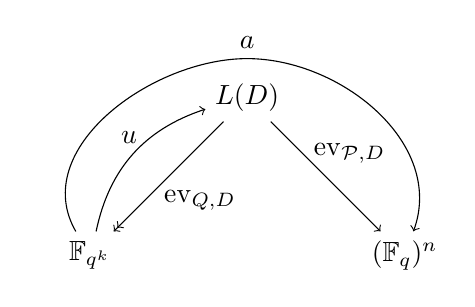
\begin{tikzpicture}
    \node (LD) at (2, 2) {$L(D)$};
    \node (Fqk) at (0, 0) {$\mathbb{F}_{q^k}$};
    \node (Fqn) at (4, 0) {$(\mathbb{F}_{q})^n$};
    \draw[->>] (LD) to (Fqk);
    \draw[->] (LD) to (Fqn);
    \draw[->] (Fqk) to[bend left] (LD);
    \node (s) at (0.5, 1.5) {$u$};
    \node (evQ) at (1.4, .7) {$\ev_{Q, D}$};
    \node (evP) at (3.3, 1.3) {$\ev_{\Pcal, D}$};
    \draw[->] (Fqk) to[out=120,in=180](2, 2.5) to[out=0, in=70] (Fqn);
    \node (a) at (2, 2.7) {$a$};
  \end{tikzpicture}
  \end{center}
Observe that $a$ is linear, so we can write
\[ a(x) = (\varphi_1(x), \dots, \varphi_n(x)) \]
where $\varphi_i:\mathbb{F}_{q^k}\to\mathbb{F}_{q}$ is a linear form, namely $\varphi_i(x)=f_x(P_i)$.

  Similarly, since the map $\ev_{\Pcal, sD}$ is injective, it admits a left inverse, \ie a linear
  map 
  \[
    r: (\mathbb{F}_{q})^n \to L(sD)
  \]
  such that 
  \[r\circ\ev_{\Pcal, sD} = \Id_{L(sD)}.
  \]
We also let $b: (\mathbb{F}_{q})^n \to \mathbb{F}_{q^k}$
  be the composite map $b = \ev_{Q, sD}\circ r$.   The situation is summed up in the
  following diagram.
  \begin{center}
  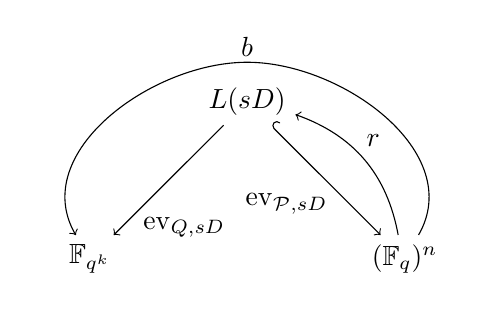
\begin{tikzpicture}
    \node (LsD) at (2, 2) {$L(sD)$};
    \node (Fqk) at (0, 0) {$\mathbb{F}_{q^k}$};
    \node (Fqn) at (4, 0) {$(\mathbb{F}_{q})^n$};
    \draw[right hook->] (LsD) to (Fqn);
    \draw[->] (LsD) to (Fqk);
    \draw[->] (Fqn) to[bend right] (LsD);
    \node (evP) at (2.5, .7) {$\ev_{\Pcal, sD}$};
    \node (s) at (3.6, 1.5) {$r$};
    \node (evQ) at (1.2, .4) {$\ev_{Q, sD}$};
    \draw[->] (Fqn) to[out=60,in=0](2, 2.5) to[out=180, in=120] (Fqk);
    \node (d) at (2, 2.7) {$b$};
  \end{tikzpicture}
\end{center}
The map $b$ is linear, so there are $b_1, \dots, b_n$ in
  $\mathbb{F}_{q^k}$ such that, for all $y=(y_1, \dots, y_n)\in(\mathbb{F}_{q})^n$,
  \[
    b(y) = \sum_{i=1}^n y_i b_i.
  \]

Now for $x,\dots,x_s\in\mathbb{F}_{q^k}$, let
  \[
    p = (p_1,\dots,p_n) = ((\prod_{j=1}^sf_{x_j})(P_1), \dots, (\prod_{j=1}^sf_{x_j})(P_n))
  \]
in $(\mathbb{F}_{q})^n$  be the coordinatewise product of the vectors $a(x_1)$, ..., $a(x_s)$.
Then
\[
  h = r(p)
\]
is an element of $L(sD)$ such that $h(P_i) = p_i = (\prod_{j=1}^sf_{x_j})(P_i)$ for all $i$.
Since the map $\ev_{\Pcal, sD}$ is injective, this forces
\[
  h = \prod_{j=1}^sf_{x_j}.
\]
Then, we have
\begin{equation*}
b(p) = \ev_{Q, sD}(r(p))
  = \ev_{Q, sD}(h)
  = h(Q)
  = \prod_{j=1}^s f_{x_j}(Q)
  = \prod_{j=1}^s x_j.
\end{equation*}
But we also have
\[
  b(p) = \sum_{i=1}^np_ib_i=\sum_{i=1}^n(\prod_{j=1}^sf_{x_j}(P_i))b_i=\sum_{i=1}^n(\prod_{j=1}^s\varphi_i(x_j))b_i
\]
and finally we get a symmetric formula for $m_s$:
\[
  \prod_{j=1}^s x_j = \sum_{i=1}^n(\prod_{j=1}^s\varphi_i(x_j))b_i.
\]
\end{proof}
Now that we have a method to find formulas, we have to prove that
Conditions~\ref{cond:hyper-1}~and~\ref{cond:hyper-2} can be satisfied.
Proposition~\ref{prop:numerical} gives sufficient assumptions to obtain these
conditions.
\begin{prop}
\label{prop:numerical}
Let $F/\mathbb{F}_{q}$ be an algebraic function field of genus $g$.
Assume that $F$ admits a place $Q$ of degree $k$, and a set $\mathcal{S}$ of
places of degree $1$ of size 
\[
  |\mathcal{S}|\geq (k+g-1)s+1.
\]
Then we have
\[ \musym_q(k,m_s)\leq ks+(g-1)(s-1). \]
\end{prop}
\begin{proof}
Set $n=ks+(g-1)(s-1)$. We will show that there are places $P_1,\dots,P_n$ in $\mathcal{S}$,
and a divisor $D$ on $F$, such that Proposition~\ref{prop:method} applies,
which gives $\musym_q(k,m_s)\leq n$ as desired.

Using e.g. \cite[Lemma~2.1]{Ballet99} we know $F$ admits a non-special divisor $R$ of degree $g-1$.
By the strong approximation theorem \cite[Thm.~1.6.5]{Stichtenoth09}
we can then find a divisor $D$ linearly equivalent to $R+Q$ and of support disjoint from $Q$ and $\mathcal{S}$.

Then $D-Q$ and $D$ are non-special, with $\ell(D-Q)=0$ and $\ell(D)=k$.
We thus find
\[
  \Ker(\ev_{Q, D}:L(D)\to\mathbb{F}_{q^k}) = L(D-Q) = 0,
\]
so $\ev_{Q, D}$ is injective, hence also surjective by equality of dimensions,
\ie the surjectivity condition~\ref{cond:hyper-1} in Proposition~\ref{prop:method} is satisfied.

Likewise, $sD$ is non-special, with $\deg(sD)=(k+g-1)s$ and $\ell(sD)=ks+(g-1)(s-1)$.
Then the evaluation map
\[
\begin{array}{cccc}
\ev_{\mathcal{S}, sD}: & L(sD) & \to & (\mathbb{F}_{q})^{|\mathcal{S}|}\\
  & h & \mapsto & (h(P))_{P\in\mathcal{S}}
\end{array}
\]
has kernel $L(sD-\sum_{P\in\mathcal{S}}P)=0$, because $\deg(sD-\sum_{P\in\mathcal{S}}P)=(k+g-1)s-|\mathcal{S}|<0$.
So $\ev_{\mathcal{S}, sD}$ is injective, with image of dimension $\dim\Img(\ev_{\mathcal{S}, sD})=\ell(sD)=n$.
Then we can find a subset $\Pcal=\{P_1,\dots,P_n\}\subset\mathcal{S}$ of size $n$,
such that $\ev_{\Pcal, sD}: L(sD) \to (\mathbb{F}_{q})^n$ is an isomorphism,
and the injectivity condition~\ref{cond:hyper-2} in Proposition~\ref{prop:method} is also satisfied.
\end{proof}

\paragraph{Choice of the curves for $q$ a large enough square.}
Now that we have somewhat easier assumptions to fulfill, that are only based on
the existence of a certain number of places, we prove that we can indeed find
algebraic function fields that satisfy these properties. We first prove it in the
special case, where the size $q$ of the base field $\K$ is a large enough
square.
\begin{prop}
\label{prop:asymptsquare}
Let $s$ be given, and assume $q$ is a square, $q\geq(s+2)^2$.
Then we have
\[
\Msym_{q,s}\leq(1+\epsilon_s(q))s
\]
with $\epsilon_s(q)=\frac{s-1}{\sqrt{q}-s-1}$.
\end{prop}
\begin{proof}
We know~\cite{STV92} that there exists a family of function fields
$F_i/\mathbb{F}_q$ of genus $g_i\to\infty$ such that
\begin{enumerate}[(i)]
  \item $\frac{g_{i+1}}{g_i}\to1$
  \item $N_i\sim (\sqrt q - 1)g_i$
\end{enumerate}
where $N_i = \Card\left\{ P\in\mathbb{P}_{F_i}\,|\,\deg P = 1 \right\}$
is the number of places of degree $1$ of $F_i$. We can also assume that the sequence
$g_i$ is increasing. 

For any $k$ let $i(k)$ be the smallest index such that
\[ N_{i(k)} \geq (k + g_{i(k)}-1)s +1. \]
Such an $i(k)$ always exists since by (ii) we have $N_i\sim (\sqrt q - 1)g_i$,
with $\sqrt q - 1>s$.

By definition we thus have
\[ N_{i(k)} \geq (k + g_{i(k)}-1)s +1 > (k + g_{i(k)-1}-1)s +1 > N_{i(k)-1}. \]
As $k\to\infty$ we have $i(k)\to\infty$, and by (i) we get 
\[
  g_{i(k)}\sim g_{i(k)-1},
\]
so by (ii) we also get 
\[
  N_{i(k)}\sim N_{i(k)-1}.
\]
This then gives
\[ \begin{split} N_{i(k)} &\sim (k + g_{i(k)}-1)s +1\\ &\sim (k + g_{i(k)})s \end{split} \]
while by (ii),
\[ N_{i(k)} \sim (\sqrt q - 1)g_{i(k)}. \]
From these two relations we deduce
\[ g_{i(k)} \sim \frac{s}{\sqrt{q}-1-t}k. \]
For $k$ large enough this implies in particular $2g_{i(k)} +1 \leq q^{(k-1)/2}(\sqrt q-1)$,
so $F_{i(k)}$ admits a place of degree $k$ by~\cite[Cor.~5.2.10]{Stichtenoth09}.

From this we are allowed to apply Proposition~\ref{prop:numerical} to $F_{i(k)}$, which gives
\[ \musym_q(k,m_s)\;\leq\; ks+(g_{i(k)}-1)(s-1)\;\sim\; ks+g_{i(k)}(s-1)\;\sim\; ks(1+\epsilon_s(q)) \]
as desired.
\end{proof}
\begin{cor}
\label{cor:asymptsquare}
For $q$ a square, $q\geq(s+3)^2$ we have
\[
\Mhyp_{q,s}\leq(1+\epsilon_{s+1}(q))(s+1),
\]
and in particular we have
\[ \Mtri_q\leq 3\left(1+\frac{2}{\sqrt{q}-4}\right) \]
for $q$ a square, $q\geq 25$.
\end{cor}

\paragraph{Conclusion for arbitrary $q$.}
Finally, we complete our objective of proving that the symmetric multilinear
complexity is linear in the degree of the extension by extending the previous
result to arbitrary $q$.

% TODO
% ====
%
% Re-write the first part of this proof. Also what happens with the linear forms
% phi_i in the proof ? They are linear forms over F_{q^{dk}} and not
% F_{q^k}. Could this be a problem?

\begin{lm}
\label{lemma:basechange}
Let $q$ be a prime power. Then for any integers $s,d,k$ we have
\[ \musym_q(k,m_s)\leq\musym_q(dk,m_s)\leq\musym_q(d,m_s)\musym_{q^d}(k,m_s). \]
\end{lm}
\begin{proof}
For the inequality on the left, there is nothing to prove if $\musym_q(dk,m_s)=\infty$.
So let us assume $m_s^{\mathbb{F}_{q^{dk}}/\mathbb{F}_{q}}$ admits a symmetric multiplication formula of length $n=\musym_q(dk,m_s)$, \ie
\[\forall x_1,\dots,x_s\in\mathbb{F}_{q^{dk}},\quad x_1\cdots x_s = \sum_{i=1}^{n}\varphi_i(x_1)\cdots\varphi_i(x_s)a_i \]
for linear forms $\varphi_i:\mathbb{F}_{q^{dk}}\to\mathbb{F}_{q}$ and elements $a_i\in\mathbb{F}_{q^{dk}}$.
Choose a linear projection
\[ p:\mathbb{F}_{q^{dk}}\to\mathbb{F}_{q^{k}} \]
left inverse for the inclusion $\mathbb{F}_{q^{k}}\subseteq\mathbb{F}_{q^{dk}}$.
Then we get
\[\forall x_1,\dots,x_s\in\mathbb{F}_{q^{k}},\quad x_1\cdots x_s = p(x_1,\dots,x_s) = \sum_{i=1}^{n}\varphi_i(x_1)\cdots\varphi_i(x_s)p(a_i) \]
which is a symmetric multiplication formula of length $n$ for $m_s^{\mathbb{F}_{q^{k}}/\mathbb{F}_{q}}$.

Likewise, for the inequality on the right, there is nothing to prove if $\musym_q(d,m_s)=\infty$ or $\musym_{q^d}(k,m_s)=\infty$.
So let us assume $m_s^{\mathbb{F}_{q^{d}}/\mathbb{F}_{q}}$ and
$m_s^{\mathbb{F}_{q^{dk}}/\mathbb{F}_{q^{d}}}$ admit symmetric multiplication
formulas of length $\rho=\musym_q(d,m_s)$ and $\mu=\musym_{q^d}(k,m_s)$ respectively, so
\vspace{-.5\baselineskip}

\[\forall y_1,\dots,y_s\in\mathbb{F}_{q^{d}},\quad y_1\cdots y_s =
\sum_{u=1}^{\rho}\psi_u(y_1)\cdots\psi_u(y_s)b_u \]
\vspace{-1.5\baselineskip}

\[\forall z_1,\dots,z_s\in\mathbb{F}_{q^{dk}},\quad z_1\cdots z_s =
\sum_{v=1}^{\mu}\chi_v(z_1)\cdots\chi_v(z_s)c_v \]
\vspace{-.5\baselineskip}

\noindent for linear forms $\psi_u:\mathbb{F}_{q^{d}}\to\mathbb{F}_{q}$, $\chi_v:\mathbb{F}_{q^{dk}}\to\mathbb{F}_{q^{d}}$ and elements $b_u\in\mathbb{F}_{q^{d}}$, $c_v\in\mathbb{F}_{q^{dk}}$.
Then setting $y_1=\chi_v(z_1)$, ..., $y_s=\chi_v(z_s)$ we find
\[\forall z_1,\dots,z_s\in\mathbb{F}_{q^{dk}},\quad z_1\cdots z_s =
\sum_{v=1}^{\mu}\sum_{u=1}^{\rho}(\psi_u\circ\chi_v)(z_1)\cdots(\psi_u\circ\chi_v)(z_s)\cdot(b_uc_v) \]
which is a symmetric multiplication formula of length $\rho\mu$ for $m_s^{\mathbb{F}_{q^{dk}}/\mathbb{F}_{q}}$.
\end{proof}


\begin{thm}
Let $s\geq2$ be an integer and $q$ a prime power.
If $q<t$, then $\musym_q(k,m_s)=\infty$ for all $k\geq2$.

On the other hand, if $q\geq s$,
then $\musym_q(k,m_s)$ grows at most linearly with $k$, \ie we have
\[
\Msym_{q,s}\leq C_s(q)
\]
for some real constant $C_s(q)<\infty$.
\end{thm}
\begin{proof}
If $q<t$ and $k\geq2$, then $\musym_q(k,m_s)=\infty$ follows from Theorem~\ref{th:criterion}.

On the other hand, for $q\geq s$, we have $\musym_q(d,m_s)<\infty$ for any integer $d$.
Choose $d$ such that $q^d$ is a square, $q^d\geq(s+2)^2$.
Then Proposition~\ref{prop:asymptsquare} shows $\musym_{q^d}(k,m_s)$ grows linearly with $k$.
The Theorem then follows thanks to Lemma~\ref{lemma:basechange}, with $C_s(q)=\musym_q(d,m_s)(1+\epsilon_s(q^d))s$.
\end{proof}
\begin{cor}
For $q\geq s+1$ we have
\[
\Mhyp_{q,s}\leq C_{s+1}(q)
\]
and in particular for $q\geq 3$ we have
\[
\Mtri_q\leq C_{3}(q).
\]
\end{cor}

%


\part{Efficient arithmetic in a lattice of finite fields}
\label{part:lattice}

\chapter{Isomorphism algorithms}
\label{chap:isomorphism}
We studied in Part~\ref{part:single} the arithmetic of a single finite field
extension. We now study a set of several extensions. The very first step will be
to understand how to compute an isomorphism (or an embedding) between two finite
fields: this is the material of this chapter.
\minitoc

% TODO: figure

\clearpage

Our reference for this chapter is~\cite{BDDFS17}: although it provides a variety
of isomorphism algorithms (and their analysis), we are mainly interested in the
naive isomorphism algorithm (used in
Chapter~\ref{chap:lattice}) and in Allombert's algorithm (used in
Chapter~\ref{chap:standard}). We thus do not cover all the isomorphism
algorithms, the reader interested in Rains' algorithm~\cite{Pinch92, Rains96}
and its elliptic variant can take a look at the paper cited above.

\section{Preliminaries and naive algorithm}
\label{sec:prelim-naive-algo}

Even if our real goal is to compute \emph{embeddings} of finite fields, \ie
ring homomorphisms
\[
  \phi:K\to L
\]
with $K$ and $L$ finite fields, we often refer to the algorithms as
\emph{isomorphism} algorithms. Indeed, computing the embedding $\phi$ is
the same as computing an isomorphism
\[
  \phi':K\overset{\sim}{\to} K'
\]
of $K$ with a subfield $K'\subset L$ of $L$. The
isomorphism $\phi'$ is just the embedding $\phi$ with its codomain being
restricted to $K'$. That is why in the remainder of this chapter, we present
\emph{isomorphism} algorithms, rather than embedding algorithms.

\subsection{Description of the problem}

We let $p$ be a prime number, $\K = \mathbb{F}_p$ be the field with $p$ elements,
and $f, g\in\K[X]$ two irreducible polynomials of degree $m=\deg(f)$ and
$n=\deg(g)$, with
\[
  m\mid n.
\]
Let
\[
  K=\K[X]/(f(X))\cong\mathbb{F}_{p^m}
\]
and
\[
  L = \K[Y]/(g(Y))\cong\mathbb{F}_{p^n}
\]
be two extensions of $\K$. We know there is an embedding
\[
  \phi:K\to L,
\]
unique up to $\K$-automorphism of $K$, \ie there are
\[
  \Card\Gal(K/\K)=m
\]
different embeddings from $K$ to $L$, that can be described as
\[
  \phi\circ\sigma
\]
for $\sigma\in\Gal(K/\K)$. Equivalently, they can also be described as
\[
  \sigma'\circ\phi
\]
with $\sigma'\in\Gal(\phi(K)/\K)$. The \emph{embedding problem} is then to
efficiently find, represent and evaluate one such embedding $\phi$. 
Following~\cite{BDDFS17}, the problem is split in two parts.
\begin{description}
  \item[Embedding description problem.] Compute elements $\alpha\in K$ and
    $\beta\in L$ such that 
    \[
      K=\K(\alpha)
    \]
    and such that there exists an embedding $\phi$ mapping $\alpha$ to $\beta$.
  \item[Embedding evaluation problem.] Given elements $\alpha$ and $\beta$
    defined above, and elements $x\in K$, $y\in L$, solve the
    following problems:
    \begin{itemize}
      \item compute $\phi(x)\in L$;
      \item test if $y\in\phi(K)$;
      \item if $y\in\phi(K)$, then compute $\phi^{-1}(y)\in K$.
    \end{itemize}
\end{description}
As the name suggests, the \emph{embedding description problem} focuses on
finding a pair of elements that are sufficient to describe an embedding. Indeed,
if 
\[
  K=\K(\alpha)
\]
we know that every element $x\in K$ can be uniquely written as 
\[
  x = \sum_{j=0}^{m-1}a_j\alpha^j
\]
with $a_j\in\K$ for al $0\leq j\leq m-1$, and the embedding $\phi$ is then
defined by
\[
  \phi(x) = \sum_{j=0}^{m-1}a_j\beta^j.
\]
\begin{prop}
  \label{prop:description}
 The elements $\alpha$ and $\beta$
 describe an embedding if and only if they have the same minimal polynomial over
 $\K$. 
\end{prop}
\begin{proof}
  Let $\phi:K\to L$ be an embedding mapping $\alpha$ to $\beta$ and let 
  \[
    P = \Minpoly_\K(\alpha)
  \]
  be the the minimal polynomial of $\alpha$. Then 
  \begin{align*}
    P(\beta) &= P(\phi(\alpha)) \\
    &= \phi(P(\alpha))\\
    &= \phi(0) \\
    &= 0
  \end{align*}
  thus $\Minpoly_\K(\beta)\neq 1$ divides $P$ which is irreducible so 
  \[
\Minpoly_\K(\beta) = P.
  \]
 Conversely, if $\alpha$ and $\beta$ have the same minimal polynomial $P$, then the
 map $\phi$ is well-defined and defines an isomorphism between the fields $\K(\alpha)$ and
 $\K(\beta)$, that are both isomorphic to the field
 \[
   \K[X]/(P(X)).
 \]
\end{proof}
While the first problem focuses on finding a description of $\phi$, the
\emph{embedding evaluation problem} independently asks how to efficiently use
the description to compute the actual embedding. We target this question in
Section~\ref{sec:evaluation}.

\subsection{Embedding description problem and naive algorithm}
\label{sec:embedding-description}

Until the end of this section and in Section~\ref{sec:allombert}, we deal with
the \emph{embedding description problem}, although we only review a subpart of
the existing algorithms (see~\cite{BDDFS17} for other algorithms). As above, let
$f$ and $g$ be two irreducible polynomials with coefficients in $\K$ and with
respective degree $m$ and $n$, such that
\[
  m\mid n.
\]
Let
\[
  K=\K[X]/(f(X))\cong\mathbb{F}_{p^m}
\]
and
\[
  L = \K[Y]/(g(Y))\cong\mathbb{F}_{p^n}
\]
be two finite fields. Then one can simply take $\alpha$ to be the class of $X$ in
$K$ and choose $\beta$ to be any root of $f$ in $L$. Indeed, we know that there
is an isomorphic copy of $K$ in $L$ and thus that $f$ splits over $L$.
Furthermore, any root of $f$ will have $f$ as its minimal polynomial, which is
also the minimal polynomial of $\alpha$ by construction. By
Proposition~\ref{prop:description}, the map 
\[
  \phi:K\to L
\]
sending $\alpha$ to $\beta$ is an embedding. The critical routine in that
algorithm is to find a root of $f$ in $L$, that can be done using the
Shoup-Kaltofen \emph{equal degree factorization} algorithm~\cite{KS97}. The
complexity analysis of~\cite{BDDFS17} indicates that the cost is strictly larger
than quasi-quadratic complexity $\tilde O(m^2)$. A more efficient algorithm, due
to Lenstra and Allombert, is discussed in Section~\ref{sec:allombert}.

\section{Lenstra-Allombert algorithm}
\label{sec:allombert}

Both Lenstra~\cite{Lenstra91} and Allombert used
Kummer theory, the study of certain field extensions, to compute isomorphisms
between finite fields. But while Lenstra's focus
was on proving the existence of a deterministic isomorphism algorithm, Allombert 
wanted to provide a practical algorithm. This led to the invention of the
Lenstra-Allombert algorithm~\cite{Allombert02} in 2002, for which we give a
description in this section. The ideas of Allombert play an important part in
Chapter~\ref{chap:standard} too. The techniques based on Kummer theory work
for extensions of degree $n$ coprime to the characteristic $p$. In order to have
an algorithm working for any type of extension, the solution is to deal with the
part of the extension which degree is divisible by $p$ separately using
Artin-Shreier theory and to glue the results together in the end. More details
can be found in~\cite[Section 3.2]{BDDFS17}.

% TODO
% ====
%
% Add an entire part on Artin-Shreier instead? Probably not, since it will not
% be used at all in the rest of the thesis.

\subsection{Preliminaries}
\label{sec:preliminaries}

Let us first discuss a simpler case than the general one, that will highlight
the method behind the Lenstra-Allombert isomorphism algorithm. Let $K$ and $L$ be
two finite fields of cardinality $p^n$, such that
\[
  K\cong L\cong \mathbb{F}_{p^n}.
\]
Assume that $\gcd(p, n)=1$ and that
\[
  n\mid p-1,
\]
or equivalently that there is a primitive $n$-th root of unity in
$\K=\mathbb{F}_p$, that we denote by $\zeta$. The algorithm is based on
Proposition~\ref{prop:h90}.

\begin{prop}[Hilbert $90$ theorem]
  \label{prop:h90}
  Let $K$ be a finite extension of $\K=\mathbb{F}_p$ of degree $n$ such that there exists a
primitive $n$-th root of unity $\zeta\in\K$ in the base field $\K$, \ie such
that $n$ divides $p-1$. 
 Let $\sigma$ be the Frobenius automorphism of the extension
 \[
   K/\K
 \]
 and consider the following equation in $K$:
 \begin{equation}
   \tag{H90}
   \sigma(x) = \zeta x.
   \label{eq:h90}
 \end{equation}
The solutions of~\eqref{eq:h90} form a one dimensional $\K$-vector space and if
$\alpha\in K$ is such a solution, we have
\[
  \alpha^n\in\K.
\]
If $\alpha$ is also nonzero, then it is a generator of $K$ over $\K$.
\end{prop}
\begin{proof}
  Let us first construct a nonzero solution of~\eqref{eq:h90}. Consider the polynomial
  \[
    P = \sum_{j=0}^{n-1}\zeta^{-j} X^{p^j}
  \]
  of degree $p^{n-1}$. The polynomial $P$ has at most $p^{n-1}$ roots in $K$,
  which has cardinality $p^n$, so there exists some element $x\in K$ such that
  \[
    y = P(x)\neq0.
  \]
  Now, by construction, we have
  \begin{align*}
    \sigma(y) &= \sigma(\sum_{j=0}^{n-1}\zeta^{-j}x^{\sigma^{j}})\\
    &= \sum_{j=0}^{n-1}\zeta^{-j}x^{\sigma^{j+1}}\\
    &= \zeta \times \sum_{j=0}^{n-1}\zeta^{-(j+1)}x^{\sigma^{j+1}}\\
    &= \zeta \times \sum_{j=1}^{n}\zeta^{-j}x^{\sigma^{j}}\\
    &= \zeta y
  \end{align*}
  and thus $y$ is a nonzero solution of~\eqref{eq:h90}. All the elements
  \[
    \lambda y
  \]
  with $\lambda\in\K$ are also solutions of~\eqref{eq:h90} since
  \[
    \sigma(\lambda y) = \lambda\sigma(y) = \zeta\lambda y,
  \]
  and the equation has at most $p$ solutions because the polynomial
  \[
    X^p - \zeta X
  \]
  has at most $p$ roots in $K$. Thus there are exactly $p$ different solutions,
  that are the elements of $\Vect(y)$. Let $z$ be a solution of~\eqref{eq:h90},
  then we have
  \begin{align*}
   \sigma(z^n) &= \sigma(z)^n\\
   &= (\zeta z)^n\\
   &= z^n,
  \end{align*}
  therefore $z^n$ is fixed by $\sigma$, which means that
  \[
    z^n\in\K.
  \]
  If $z$ is also nonzero, then for all $0\leq j<n$, we have
  \begin{align*}
    \sigma^j(z) &= \underbrace{(\sigma\circ\dots\circ\sigma)}_{j\text{ times}}(z)\\
    &= \underbrace{(\sigma\circ\dots\circ\sigma)}_{j-1\text{ times}}(\zeta z)\\
    &= \zeta\underbrace{(\sigma\circ\dots\circ\sigma)}_{j-1\text{ times}}(z)\\
    &= \zeta^j z\\
    &\neq z.
  \end{align*}
  Consequently, $z$ is not in any subfield of $K$ and is thus a generator of $K$
  over $\K$.
\end{proof}
Note that Proposition~\ref{prop:h90} applies both to the fields $K$ and $L$,
therefore we can solve Equation~\eqref{eq:h90} in both fields. Let $\alpha_K$ be a
solution of Equation~\eqref{eq:h90} for the root $\zeta$ in $K$, and $\alpha_L$
a solution in $L$. Since we want the primitive $n$-th root of unity $\zeta$ to
be the same in $K$ and $L$, we assume that we already have an embedding from
$\K$ in both these fields. In practice, since $\K$ is a
prime field and the fields $K$ and $L$ are represented by polynomials over
$\K = \mathbb{F}_p=\mathbb{Z}/p\mathbb{Z}$, the assumption is not really
hard to meet. Let
\[
  a_K = \alpha_K^n
\]
and
\[
  a_L = \alpha_L^n.
\]
By Proposition~\ref{prop:h90}, we know that $a_K$ and $a_L$ are both in $\K$ and
this can be used to compute an isomorphism between $K$ and $L$.
\begin{prop}[Allombert~{\cite{Allombert02}}]
  \label{prop:allombert-simple}
 The quotient
 \[
   a_K/a_L
 \]
 is an $n$-th power in $\K$, and if
 \[
   c^n = a_K/a_L
 \]
 then the map sending $\alpha_K$ to $c\alpha_L$ is an isomorphism from $K$ to $L$.
\end{prop}
\begin{proof}
  Let $\phi:K\to L$ be a $\K$-isomorphism between $K$ and $L$. We have
  \begin{align*}
    \sigma(\phi(\alpha_K)) &= \phi(\alpha_K)^p\\
    &= \phi(\alpha_K^p)\\
    &= \phi(\sigma(\alpha_K))\\
    &= \phi(\zeta\alpha_K)\\
    &= \zeta\phi(\alpha_K)
  \end{align*}
  thus $\phi(\alpha_K)$ is a solution of~\eqref{eq:h90} and by
  Proposition~\ref{prop:h90} there exists $\lambda\in\K$ such that
  \[
    \phi(\alpha_K) = \lambda\alpha_L.
  \]
  We also have
  \[
    \phi(\alpha_K)^n = \phi(\alpha_K^n) = \phi(a_K) = a_K,
  \]
  therefore the quotient
  \begin{align*}
    a_K/a_L &= \phi(\alpha_K)^n/\alpha_L^n\\
    &= \lambda^{n}
  \end{align*}
  is an $n$-th power in $\K$. Now let $c\in\K$ be any $n$-th root of $a_K/a_L$,
  then
  \[
    c = \zeta^j\lambda
  \]
  for some $0\leq j\leq n-1$, that is $c$ and $\lambda$ differ by a $n$-th root
  of unity, and so do $\phi(\alpha_K)$ and $c\alpha_L$:
  \[
    c\alpha_L = \zeta^j\phi(\alpha_K) = \sigma^j(\phi(\alpha_K)).
  \]
  Finally, the elements $c\alpha_L$ and $\phi(\alpha_K)$ have the same minimal
  polynomial, because they are conjugates, and $\phi(\alpha_K)$ has the same
  minimal polynomial as $\alpha_K$ because $\phi$ is an isomorphism, so by
  Proposition~\ref{prop:description}, the map sending $\alpha_K$ to $c\alpha_L$ is an
  isomorphism from $K$ to $L$.
\end{proof}
In this simpler case ($n$ divides $p-1$), Lenstra-Allombert algorithm consists
in
\begin{enumerate}
  \item finding $\alpha_K\in K$ and $\alpha_L\in L$ with
    $\sigma(\alpha_K)=\zeta\alpha_K$ and $\sigma(\alpha_L)=\zeta\alpha_L$;
  \item computing a $n$-th root $c\in\K$ of $\alpha_K^n/\alpha_L^n$;
  \item returning the isomorphism described by $\alpha_K\mapsto c\alpha_L$.
\end{enumerate}

\paragraph{General case.} When $n\nmid p-1$, which is always
the case asymptotically since we work with $p$ fixed and we let $n$ grow, there
are no $n$-th roots of unity in $\K$, and the strategy of
Section~\ref{sec:preliminaries} cannot be applied as if. Nevertheless, it is
still possible to apply a similar idea by extending the space so that it
contains artificial roots of unity.

\subsection{Kummer algebras}
\label{sec:kummer-algebras}

% TODO
% ====
%
% Fix the definitions by saying something about where do we pick the roots of
% unity from. Algebraic closure ? Doesn't that make some of the results trivial or
% something? 

Instead of ``just'' working in $\mathbb{F}_{p^n}$, we work in
\[
  A_n = \mathbb{F}_{p^n}\otimes \mathbb{F}_p(\zeta),
\]
where $\zeta$ is a primitive $n$-th root of unity, and where $\otimes$ is the tensor
product over $\K=\mathbb{F}_p$. We thus extend the scalars and force the existence of
suitable roots of unity. The $\K$-algebra $A_n$ can now be used instead of
$\mathbb{F}_{p^n}$ in the Lenstra-Allombert algorithm. Following the terminology
of~\cite{DRR19}, we call these algebras \emph{Kummer algebras}.

\begin{defi}[Kummer algebra]
  Let $p\in\mathbb{N}$ a prime number and $\K=\mathbb{F}_p$ the finite field
  with $p$ elements.
 We call the $\K$-algebra
 \[
   A_n = \mathbb{F}_{p^n}\otimes\mathbb{F}_{p}(\zeta),
 \]
 where $\otimes$ is the tensor product over $\K$, a \emph{Kummer algebra of
 degree $n$}.
\end{defi}
\begin{defi}[Field of scalars]
  Let $A_n$ be a Kummer algebra of degree $n$. Then we define
  $\mathbb{F}_{p}(\zeta)$ as the \emph{field of scalars} of $A_n$, and we
  define the \emph{level} $\nu(n)$ of $A_n$ as
  \[
    \nu(n) = \mathrm{ord}_{(\mathbb{Z}/n\mathbb{Z})^\times}(p) = \left[
      \mathbb{F}_{p}(\zeta):\K \right],
  \]
  where $\mathrm{ord}_{(\mathbb{Z}/n\mathbb{Z})^\times}(p)$ is the order of $p$
  in the multiplicative group $(\mathbb{Z}/n\mathbb{Z})^\times$. The level
  $\nu(n)$ of $A_n$ is the degree of its field of scalars.
\end{defi}
Let $\sigma:x\mapsto x^p$ be the Frobenius automorphism of the extension
\[
  \mathbb{F}_{p^n}/\K,
\]
and extend it to $A_n$ by defining the linear map
\[
  \begin{array}{cccc}
    \sigma\otimes 1: & A_n & \to & A_n\\
    & \sum_j x_j\otimes y_j & \mapsto & \sum_j \sigma(x_j) \otimes y_j.
  \end{array}
\]
The map $\sigma\otimes 1$ will play the role of $\sigma$ in the simpler case.
\begin{lm}
  The map $\sigma\otimes1$ is a $1\otimes\mathbb{F}_{p}(\zeta)$-linear
  endomorphism with $n$ distinct eigenvalues, that are the powers of
  $1\otimes\zeta$.
\end{lm}
\begin{proof}
  Because of the linear independence of characters~\cite[Chapter VI,
  §4]{Lang04}, we know that the automorphisms
  \[
    \Id, \sigma, \sigma^2, \dots, \sigma^{n-1}
  \]
  are independent. We also know that 
  \[
    \sigma^n = \Id,
  \]
  therefore the minimal polynomial of the $\K$-linear endomorphism $\sigma$ is
  \[
    X^n-1.
  \]
  By the Cayley-Hamilton theorem, we deduce that the characteristic
  polynomial of $\sigma$ is also $X^n-1$. Now let $\B=\left\{ b_1, \dots, b_n \right\}$ be a basis of
  $\mathbb{F}_{p^n}/\K$ and let $M$ be the matrix of $\sigma$ in this basis.
  Then the matrix of the $1\otimes\mathbb{F}_p(\zeta)$-linear endomorphism
  $\sigma\otimes1$ in the basis
  \[
    \B\otimes 1 =\left\{ b_1\otimes1, \dots, b_n\otimes1 \right\}
  \]
  is also $M$. Thus, the characteristic polynomial of $\sigma\otimes1$ is again
  $X^n-1$, that splits completely in 
  \[
    1\otimes\mathbb{F}_{p}(\zeta)\cong \mathbb{F}_{p}(\zeta),
  \]
  the roots being the elements
  \[
    1\otimes\zeta^j
  \]
  for $0\leq j\leq n-1$. Finally, the eigenvalues are the roots of the
  characteristic polynomial so this concludes the proof.
\end{proof}
Since there are exactly $n$ distinct eigenvalues, we know that the
corresponding eigenspaces are all one-dimensional
$1\otimes\mathbb{F}_{p}(\zeta)$-vector spaces, and the eigenspace corresponding
to the eigenvalue $\zeta$ is described by the equation
 \begin{equation}
   \tag{H90}
   (\sigma\otimes1)(x) = (1\otimes\zeta) x
   \label{eq:h90-kummer}
 \end{equation}
 that we again denote by~\eqref{eq:h90-kummer}. The field of scalars of $A_n$ now
 plays the role of the base field $\K$ in the simpler case and the solutions
 of~\eqref{eq:h90-kummer} have similar properties.
 \begin{lm}
   \label{lm:fixed-elems}
   The set of elements in $A_n$ fixed by $\sigma\otimes1$ is
   \[
     1\otimes\mathbb{F}_{p}(\zeta)\cong \mathbb{F}_{p}(\zeta),
   \]
   a subfield isomorphic to the field of scalars of $A_n$.
 \end{lm}
 \begin{proof}
   Let 
   \[
     \B = \left\{ b_1, \dots, b_a \right\}
   \]
   be a basis of
   \[
     \mathbb{F}_p(\zeta)/\K.
   \]
   Then, every element $\alpha$ in $A_n$ can be uniquely written in the form
   \[
     \alpha = \sum_{j=1}^a x_j\otimes b_j
   \]
   where for all $1\leq j\leq a$, $x_j\in\mathbb{F}_{p^n}$. If 
   \begin{align*}
     \sum_{j=1}^a\sigma(x_j)\otimes b_j &= (\sigma\otimes1)(\alpha)\\
     &= \alpha
   \end{align*}
 it follows that for all $1\leq j\leq a$, we have
   \[
     \sigma(x_j) = x_j
   \]
   and thus we have $x_j\in\K$. Consequently, the element $\alpha$ belongs to
   the set
   \[
     \K\otimes\mathbb{F}_{p}(\zeta) =
     1\otimes\mathbb{F}_p(\zeta)\cong\mathbb{F}_p(\zeta).
   \]
   Conversely, if an element $\alpha$ is in $1\otimes\mathbb{F}_{p}(\zeta)$,
   then it is fixed by $\sigma\otimes1$.
 \end{proof}
 \begin{rem}
   \label{rem:fixed-elems}
   We can use the proof of Lemma~\ref{lm:fixed-elems}, \emph{mutatis mutandis},
   in order to prove that the set of elements in $A_n$ fixed by
   $1\otimes\sigma'$, with $\sigma'$ the Frobenius automorphism of the extension
   $\mathbb{F}_{p}(\zeta)/\K$, is $\mathbb{F}_{p^n}\otimes1$. In the remainder
   of the document, we write $\sigma$ for both $\sigma$ and $\sigma'$.
 \end{rem}
 \begin{lm}
   \label{lm:h90-solutions}
   Let $\alpha$ be a nonzero solution of~\eqref{eq:h90-kummer} for the root
   $\zeta$. Then 
   \[
     \alpha^n\in 1\otimes\mathbb{F}_{p}(\zeta)
   \]
   and $\alpha$ is a generating element for $A_n$ as an algebra over
   $1\otimes\mathbb{F}_{p}(\zeta)$ that is also invertible.
 \end{lm}
 \begin{proof}
  We have
  \begin{align*}
    (\sigma\otimes1)(\alpha^n) &= (\sigma\otimes1)(\alpha)^n\\
    &= ((1\otimes\zeta)\alpha)^n\\
    &= (1\otimes\zeta^n)\alpha^n\\
    &= \alpha^n,
  \end{align*}
  thus $\alpha^n\in1\otimes\mathbb{F}_p(\zeta)$ by Lemma~\ref{lm:fixed-elems}.
  Since $\alpha$ is a solution of~\eqref{eq:h90-kummer} for $\zeta$, then
  for every $1\leq j\leq n-1$, $\alpha^j$ is a solution for $\zeta^j$, indeed
  \begin{align*}
    (\sigma\otimes 1)(\alpha^j) &= ( (\sigma\otimes1)(\alpha))^j\\
    &= (1\otimes\zeta^j)\alpha^j.
  \end{align*}
  Then, the elements $1, \alpha, \dots, \alpha^{n-1}$ are eigenvectors for
  distinct eigenvalues of $\sigma\otimes1$ and thus form a basis of $A_n$ over
  $1\otimes \mathbb{F}_{p}(\zeta)$. Assume that $\alpha^n=1\otimes c$ for some
  $c\in\mathbb{F}_{p}(\zeta)$. There are no nonzero nilpotent elements in $A_n$;
  one way of seeing it is to say that
  \[
    A_n \cong \mathbb{F}_{p}(\zeta)[T]/(h(T))
  \]
  where $h$ is the irreducible polynomial defining
  \[
    \mathbb{F}_{p^n} = \K[X]/(h(X)).
  \]
  Since the degree $n$ of
  $h$ is not a multiple of $p$, the polynomial $h$ is separable and 
  \[
    \mathbb{F}_{p^n}[T]/(h(T))
  \]
  has no nonzero nilpotent elements. Then $\alpha^n$ is nonzero thus
  $c\in\mathbb{F}_p(\zeta)$ is also nonzero. It follows that $\alpha$ is
  invertible, indeed
  \[
    \alpha^{-1} = (1\otimes c^{-1})\alpha^{n-1}.
  \]
 \end{proof}
 \begin{defi}[Kummer constant]
   Let $\alpha\in A_n$ be a nonzero solution of~\eqref{eq:h90-kummer} for the
   root $\zeta$. The constant $c\in\mathbb{F}_p(\zeta)$ such that
   \[
     \alpha^n = 1\otimes c
   \]
   is called the \emph{Kummer constant} of $\alpha$.
 \end{defi}
 One key property of the solutions of~\eqref{eq:h90-kummer} is still missing,
 and we need a new notation to express it. Let $K$ and $L$ be two finite field
 extensions of $\K$ and let $\mu\in L$ be an element of degree $d$ over $\K$. As
 used several times already, we know that an element 
 \[
   \beta\in K\otimes \K(\mu)\subset K\otimes L 
 \]
   can be uniquely written as
 \[
   \beta=\sum_{j=0}^{d-1}x_j\otimes\mu^j,
 \]
 and we set
 \[
   \first{\beta}{\mu} = x_0.
 \]
 \begin{prop}[{\cite[Proposition 3.6]{Allombert02}}]
   \label{prop:generate}
   Let $\alpha$ be a nonzero solution of~\eqref{eq:h90-kummer} for the root
   $\zeta$, then
   \[
     \first{\alpha}{\zeta}
   \]
   is a generating element of the extension
   \[
     \mathbb{F}_{p^n}/\K.
   \]
 \end{prop}
 \begin{proof}
   Let $r=\left[ \mathbb{F}_{p}(\zeta):\K \right]$ and
   \[
     P = X^r - \sum_{j=0}^{r-1}z_j X^j
   \]
   the minimal polynomial of $\zeta$ over $\K$. Let also
   \[
     \alpha = \sum_{j=0}^{r-1}a_j\otimes\zeta^j.
   \]
   It follows that 
   \begin{align*}
     \sum_{j=0}^{r-1}\sigma(a_j)\otimes\zeta^j &=(\sigma\otimes1)(\alpha)\\
     &= (1\otimes\zeta)\alpha\\
     &= \sum_{j=0}^{r-1}a_j\otimes\zeta^{j+1}\\
     &= \sum_{j=0}^{r-2}a_j\otimes\zeta^{j+1} +
     a_{r-1}\otimes(\sum_{i=0}^{r-1}z_i\zeta^i)\\
     &= a_{r-1}z_0\otimes 1 +
     \sum_{j=1}^{r-1}(a_{j-1}+a_{r-1}z_j)\otimes\zeta^j,
   \end{align*}
   we thus have
   \[
   \left\{ 
     \begin{array}{l}
       \sigma(a_0) = a_{r-1}z_0 \\
       \sigma(a_j) = a_{j-1}+a_{r-1}z_j\text{ for all }1\leq j\leq r-1.
     \end{array}
   \right.
 \]
 With these equations, we will prove that
 \[
   \mathbb{F}_p(a_0) = \mathbb{F}_{p^n},
 \]
 thus concluding the proof. We have $\sigma(a_0)\in\mathbb{F}_p(a_0)$ and
 $z_0\in\K$. Since $z_0$ is nonzero, we have that
 \[
   a_{r-1} = \sigma(a_0)z_0^{-1}\in\mathbb{F}_p(a_0).
 \]
 Going from $j=r-1$ down to $1$, it also follows that
 $a_{j-1}\in\mathbb{F}_{p}(a_0)$. Now assume that $e\in\mathbb{N}$ is an integer
 such that
 \[
   \sigma^e(x) = x
 \]
 for all $x\in\mathbb{F}_p(a_0)$, and such that $e<n$, \ie
 \[
   \mathbb{F}_p(a_0)\subsetneq \mathbb{F}_{p^n}.
 \]
 Since all the $a_j$ are in $\mathbb{F}_{p}(a_0)$, we also have
 \begin{align*}
  (1\otimes\zeta^e)\alpha &= (\sigma\otimes1)^e(\alpha)\\
  &= (\sigma^e\otimes1)(\alpha)\\
  &= \alpha
 \end{align*}
 and thus $\zeta^e=1$, which is a contradiction since $\zeta$ is a primitive
 $n$-th root of unity and $e<n$. Therefore we must have $e=n$ and
 $\mathbb{F}_p(a_0) = \mathbb{F}_{p^n}$.
 \end{proof}
 \begin{rem}
   \label{rem:recover-alpha}
 With the equations 
    \[
   \left\{ 
     \begin{array}{l}
       \sigma(a_0) = a_{r-1}z_0 \\
       \sigma(a_j) = a_{j-1}+a_{r-1}z_j\text{ for all }1\leq j\leq r-1
     \end{array}
   \right.
 \]
 found in the proof of Proposition~\ref{prop:generate}, we note that we can in
 fact also recover $\alpha$ from $\first{\alpha}{\zeta}$.
 \end{rem}
Similarly to the case where $n\mid p-1$, where the solutions
$\alpha\in\mathbb{F}_{p^n}$ of~\eqref{eq:h90} directly generate $\mathbb{F}_{p^n}$, we now know
that the solutions $\alpha\in A_n$ of~\eqref{eq:h90-kummer} in the general case
can also be used to generate $\mathbb{F}_{p^n}$ through $\first{\alpha}{\zeta}$.
We can study these solutions a bit further: in fact the element
$\first{\alpha}{\zeta}$ essentially depends on $\alpha^n$, rather than on
$\alpha$.
\begin{prop}
  \label{prop:kummer-constant}
  Let
  \[
    \alpha=\sum_{j=0}^{r-1}a_j\otimes\zeta^j\in A_n
  \]
  be a nonzero solution of~\eqref{eq:h90-kummer} for $\zeta$ and
  let $\alpha^n = 1\otimes c$. There are exactly $n$ elements $x\in A_n$ that
  are solutions of~\eqref{eq:h90-kummer} for $\zeta$ and such that
  \[
    x^n = 1\otimes c.
  \]
  These elements are the
  \[
    (1\otimes\zeta^u)\alpha = (\sigma^u\otimes1)(\alpha)
  \]
  for $0\leq u\leq n-1$. The corresponding generating elements of
  $\mathbb{F}_{p^n}/\K$ are the
  \[
    \first{(\sigma^u\otimes1)(\alpha)}{\zeta} = \sigma^u(a_0);
  \]
  they all have the same minimal polynomial, which is an irreducible polynomial
  defining $\mathbb{F}_{p^n}/\K$ that only depends on the Kummer constant
  $c\in\mathbb{F}_{p}(\zeta)$.
\end{prop}
\begin{proof}
  The solutions of~\eqref{eq:h90-kummer} form a one-dimensional
  $1\otimes\mathbb{F}_p(\zeta)$-vector space, so all solutions are of the form
  \[
    x = (1\otimes\lambda)\alpha
  \]
  with $\lambda\in\mathbb{F}_p(\zeta)$.
  Since we also ask for $x^n = \alpha^n$, we must have $\lambda^n = 1$ and thus 
  \[
    \lambda = \zeta^u
  \]
  for some $0\leq u\leq r-1$. Conversely all the solutions of the form
  $x=(1\otimes\zeta^u)$ verify $x^n=\alpha^n$. Therefore, if $x$ is such an
  element, we have
  \begin{align*}
    x &= (\sigma^u\otimes1)(\alpha)\\
    &= \sum_{j=0}^{r-1}\sigma^u(a_j)\otimes\zeta^j,
  \end{align*}
  thus
  \[
    \first{x}{\zeta} = \sigma^u(a_0).
  \]
  All these elements are conjugates, thus share the same minimal polynomial,
  that is known to define $\mathbb{F}_{p^n}/\K$ by
  Proposition~\ref{prop:generate} and that depends only on the constant
  $c\in\mathbb{F}_p(\zeta)$.
\end{proof}

\subsection{The isomorphism algorithm}
\label{sec:lenstra-allombert-isomorphism}

Let $p\in\mathbb{N}$ a prime number and $n\in\mathbb{N}$ be an integer such that
$\gcd(n, p)=1$. Let $K$ and $L$ be two finite fields of cardinality $p^n$, such
that
\[
  K\cong L\cong \mathbb{F}_{p^n}.
\]
Let $\zeta$ be a primitive $n$-th root of unity. In this section, we show how to
construct a single isomorphism between $K$ and $L$, using the results of
Section~\ref{sec:kummer-algebras}. How to construct embeddings
between extensions of different degrees, and how to deal with a lattice of
embeddings, is discussed in~Chapter~\ref{chap:standard}, together with
additionnal results on Kummer algebras. We let
\[
  A_K = K\otimes\mathbb{F}_p(\zeta)
\]
and
\[
  A_L = L\otimes\mathbb{F}_{p}(\zeta)
\]
be the two Kummer algebras constructed with $K$ and $L$ and with the same field of
scalars $\mathbb{F}_{p}(\zeta)$. The next proposition is the generalization of
Proposition~\ref{prop:allombert-simple}.
\begin{prop}
  \label{prop:lenstra-allombert-algorithm}
 Let $\alpha_K\in A_K$ (respectively $\alpha_L\in A_L$) be a nonzero solution
 of~\eqref{eq:h90-kummer} for the root $\zeta$ in the Kummer algebra $A_K$
 (resp. $A_L$) and let $c_K\in\mathbb{F}_{p}(\zeta)$ (resp.
 $c_L\in\mathbb{F}_p(\zeta)$) the Kummer constant of $\alpha_K$
 (resp. $\alpha_L$). The quotient
 \[
   c_K/c_L
 \]
 is a $n$-th power in $\mathbb{F}_p(\zeta)$, and if
 \[
   \kappa^n = c_K/c_L
 \]
 then the map sending $\first{\alpha_K}{\zeta}$ to
 $\first{(1\otimes\kappa)\alpha_L}{\zeta}$ is an isomorphism from $K$ to $L$.
\end{prop}
\begin{proof}
  The proof is very similar to the one of
  Proposition~\ref{prop:allombert-simple}. Let
  \[
    \phi:K\to L
  \]
  be an isomorphism from $K$ to $L$. Then $\phi\otimes1$ is a morphism of
  algebras from $A_K$ to $A_L$ and
  \[
    (\phi\otimes1)(\alpha_K)
  \]
  is a solution of~\eqref{eq:h90-kummer} for $\zeta$ in $A_L$. Therefore
  there exist $\lambda\in\mathbb{F}_p(\zeta)$ such that
  \[
    (\phi\otimes1)(\alpha_K) = \lambda\alpha_L.
  \]
  The Kummer constant of $(\phi\otimes1)(\alpha_K)$ is still $c_K$, and we have
  \[
    c_K/c_L = \lambda^n.
  \]
  Hence, if $\kappa$ is an $n$-th root of $c_K/c_L$, we have
  \[
    ((1\otimes\kappa)\alpha_L)^n = c_K,
  \]
  \ie the elements $\alpha_K$ and $(1\otimes\kappa)\alpha_L$ share the same
  Kummer constant. By Proposition~\ref{prop:kummer-constant}, the elements
  $\first{\alpha_K}{\zeta}$ and $\first{(1\otimes\kappa)\alpha_L}{\zeta}$ have
  the same minimal polynomial and thus describe an isomorphism from $K$ to $L$
  by Proposition~\ref{prop:description}.
\end{proof}
Finally, Lenstra-Allombert algorithm, in the general case, consists in
\begin{enumerate}
  \item finding $\alpha_K\in K\otimes\mathbb{F}_p(\zeta)$ such that
    \[
      (\sigma\otimes1)(\alpha_K)=(1\otimes\zeta)\alpha_K
    \]
    and $\alpha_L\in L\otimes\mathbb{F}_p(\zeta)$ such that
    \[
      (\sigma\otimes1)(\alpha_L)=(1\otimes\zeta)\alpha_L;
    \]
  \item computing an $n$-th root $\kappa\in\mathbb{F}_p(\zeta)$ of the quotient
    $\alpha_K^n/\alpha_L^n$;
  \item returning the isomorphism described by
    $\first{\alpha_K}{\zeta}\mapsto\first{(1\otimes\kappa)\alpha_L}{\zeta}$.
\end{enumerate}
The computational cost of Lenstra-Allombert algorithm resides in the computation
of~\eqref{eq:h90-kummer} solutions, \ie Step $1$ of the previous list.

\subsection{Computing~\eqref{eq:h90-kummer} solutions}
\label{sec:computing-h90}

In this section, we briefly present the different known solutions to
compute~\eqref{eq:h90-kummer} solutions, details can be found in~\cite{BDDFS17}.
Allombert first proposed to use linear
algebra. The idea is to compute the matrix $M$ of the Frobenius automorphism
$\sigma$ of $\mathbb{F}_{p^n}/\K$, that is the same as the matrix of
$\sigma\otimes1$, and then to compute an eigenvector of $M$ over
\[
  1\otimes\mathbb{F}_{p}(\zeta) \cong \mathbb{F}_{p}(\zeta)
\]
for the eigenvalue
\[
  1\otimes\zeta\cong\zeta.
\]
Allombert later revised his algorithm~\cite{Allombert02, Allombert02-rev}:
instead of directly using linear algebra over
$\mathbb{F}_{p}(\zeta)$, we can use the factorization
\[
  P(X) = (X-\zeta)b(X)
\]
where $P$ is the minimal polynomial of $\zeta$ over $\K$. If we write 
\[
  P = X^r + \sum_{j=0}^{r-1}z_jX^j,
\]
we can check that
\[
  b(X) = \sum_{j=0}^{r-1}b_j(X)\zeta^j,\text{ where}
  \left\{ 
    \begin{array}{l}
      b_{r-1}(X) = 1,\\
      b_{j-1}(X) = b_j(X) X + z_j\text{ for all } 0\leq j\leq r-1.
    \end{array}
  \right.
\]
Indeed, direct computation shows that
\[
  (X-\zeta)b(X) = b_0(X)X+z_0  = b_{-1}(X)
\]
and Horner 's rule also shows that
\[
  b_{-1}(X) = P(X).
\]
We then get a solution of~\eqref{eq:h90-kummer} by evaluating $b(X)$ at an
element in the kernel of 
\[
  P(\sigma)=(\sigma-\zeta\Id)\circ b(\sigma),
\]
hence we still use linear algebra, but
over $\K=\mathbb{F}_p$ instead of $\mathbb{F}_{p}(\zeta)$ this time. A different
strategy follows from the fact that if $x\in\mathbb{F}_{p^n}$, then
\[
  \alpha_x=\sum_{j=0}^{n-1}\sigma^j(x)\otimes\zeta^{-j-1}
\]
verifies
\[
  (\sigma\otimes1)(\alpha_x) = (1\otimes\zeta)\alpha_x.
\]
This is also a consequence of the factorization
\begin{align*}
  X^n-1 &= (X-\zeta)\sum_{j=0}^{n-1}\zeta^{-j-1}X^j\\
  &= (X-\zeta)\Theta(X).
\end{align*}
The question is now whether the solution $\alpha_x$ is nonzero. By the theorem
on character independence~\cite[Chapter VI, §4]{Lang04} the maps
$1, \sigma, \sigma^2, \dots, \sigma^{n-1}$, all distinct, are independent.
Therefore, the $\K$-linear map
\[
  x\mapsto\alpha_x
\]
cannot be indentically zero on $\mathbb{F}_{p^n}$ and has rank at least $1$. A
random $\alpha_x$ thus has a probability of being zero less than $1/p$, so we
need $O(1)$ trials to find a nonzero $\alpha_x$ at random. Depending on the
relative size of $p$, $n$, and $s=\left[ \mathbb{F}_p(\zeta):\K \right]$, the
computational cost of finding a nonzero $\alpha_x$ is discussed in details
in~\cite{BDDFS17} and is bounded by $O(M(n^2)\log(n)+M(n)\log(p))$. If
$\omega=3$, where $\omega$ is the exponent of matrix
multiplication, then the cost is at best quadratic in $n$.

\section{The embedding evaluation problem}
\label{sec:evaluation}

Let us first recall the problem. Let $\K=\mathbb{F}_p$ the prime field with $p$
elements, where $p\in\mathbb{N}$ is a prime number, and let $K$ and $L$ be
two finite extensions of $\K$. Let $m=\left[ K:\K \right]$ and $n = \left[ L:\K
\right]$ be the respective degrees of the extensions $K/\K$ and $L/\K$ and
assume that
\[
  m\mid n.
\]
Let $\alpha\in K$ and $\beta\in L$ be two elements such that the $\K$-linear map
\[
  \phi:\alpha\mapsto\beta
\]
sending $\alpha$ to $\beta$ describes an embedding from $K$ to $L$. The
\emph{embedding evaluation problem} consists in three sub-goals: given $\alpha$
and $\beta$ defined above and elements $\gamma\in K$, $\delta\in L$:
\begin{itemize}
  \item compute $\phi(\gamma)\in L$;
  \item test if $\delta\in\phi(K)$;
  \item if $\delta\in\phi(K)$, then compute $\phi^{-1}(\delta)\in K$.
\end{itemize}
In this section too, we follow the presentation of~\cite{BDDFS17} and we develop
three solutions constructed on top of each other.

\subsection{Linear algebra}
\label{sec:linalg}

Until the end of the section, we assume that the elements in $K$ are represented
on the monomial basis
\[
  (1, X, \dots, X^{m-1})
\]
and the elements in $L$ are represented on the monomial basis
\[
  (1, Y, \dots, Y^{n-1}).
\]
We are particularly interested in the $\K$-vector space structure of $K$ and
$L$ and in order to emphasize which basis is used, we let
\[
  V_X
\]
be the vector space $K$ equipped with the basis $(1, X, \dots, X^{m-1})$ and
\[
  V_Y
\]
be the vector space $L$ equipped with the basis $(1, Y, \dots, Y^{n-1})$.
Similarly, we let 
\[
  V_\alpha
\]
be the vector space $K$ equipped with the basis $(1, \alpha, \dots,
\alpha^{m-1})$ and
\[
  V_\beta
\]
be the subspace $V_\beta\subset L$ equipped with the basis $(1, \beta, \dots,
\beta^{m-1})$, that is isomorphic to $V_\alpha$.
Since the map $\phi$ is $\K$-linear, we can store the $n\times m$ matrix representing $\phi$
in the monomial bases and evaluate $\phi$ via a matrix-vector product. We know
that $\phi$ maps $\alpha$ to $\beta$, hence we write $\phi$ as the composition
of three maps
\[
  V_X \overset{\sim}{\longrightarrow} V_\alpha \overset{\sim}{\longrightarrow}
  V_\beta \longhookrightarrow V_Y.
\]
First, we apply a change of basis from $V_X$ to $V_\alpha$. Then we apply the
isomorphism from $V_\alpha$ to $V_\beta$, that is represented by the
identity matrix. Finally we write the obtained element, expressed in $(1,
\beta, \dots, \beta^{m-1})$, in the
monomial basis of $L$, \ie we embed $V_\beta$ in $V_Y$. The map
$V_\beta\hookrightarrow V_Y$ is represented by an $n\times m$ matrix whose
columns are the vectors $(\beta^j)_{0\leq j\leq m-1}$ expressed in the monomial
basis of $L$. The inverse of this map is obtained by solving a linear system.
Similarly, the map $V_X\overset{\sim}{\to}V_\alpha$ is represented
by the $m\times m$ matrix whose columns are the vectors $(X^j)_{0\leq j\leq
m-1}$ expressed in the basis $(1, \alpha, \dots, \alpha^{m-1})$, that is also
the inverse of the matrix whose columns are the vectors $(\alpha^j)_{0\leq j\leq
m-1}$ expressed in the monomial basis of $K$. The cost of the evaluation of
$\phi$ and its inverse is thus dominated by the solving of the linear system,
that is $O(m^{\omega-1}n)$. This cost can be reduced to $O(mn)$ with some
precomputation, \eg an LU decomposition, but the biggest drawback of the linear
algebra approach is the memory complexity rather than the time complexity.
Indeed, storing the matrices requires $O(mn)$ elements in $\K$.

\subsection{Inverse maps and duality}
\label{sec:duality}

The first improvement to the linear algebra method consists in replacing the
linear system solving used in the computation of the inverse of
\[
  V_\beta\emb V_Y
\]
by simpler operations, such as matrix-vector product, in order to reduce the
overall complexity. We first recall facts about bilinear forms and duality, the
presentation follows the one in~\cite{BDDFS17} and~\cite{DDS14}, and a standard
presentation is also available in~\cite{Lang04}. Recall that
\[
  K\cong\mathbb{F}_{p^m}
\]
admits a monomial basis $(1, X, \dots, X^{m-1})$ and that
\[
  L\cong\mathbb{F}_{p^n}
\]
admits a monomial basis $(1, Y, \dots, Y^{n-1})$. The trace $\tr_{K/\K}$ from $K$ to
$\K$ defines a non-degenerate bilinear form denoted by
\[
  \ps{x}{y}_K = \tr_{K/\K}(xy).
\]
Therefore, we can define a \emph{dual basis} $(X_0^*, X_1^*, \dots, X_{m-1}^*)$
to $(1, X, \dots, X^{m-1})$, characterized by
\[
  \ps{X^j}{X_i^*}=\left\{\begin{array}{l}
    1\text{ if }i=j\\
    0\text{ otherwise.}
  \end{array}\right.
\]
Similarly, we can define a non-degenerate bilinear form from $L$ to $\K$ by
\[
  \ps{x}{y}_L = \tr_{L/\K}(xy),
\]
and a dual basis $(Y_0^*, \dots, Y_{n-1}^*)$ to $(1, \dots, Y^{n-1})$
corresponding to this bilinear form. Now, let
\[
  \psi:K\emb L
\]
be an embedding. It is a $\K$-linear map and thus there exists a unique
\emph{dual map} $\psi^t$, such that
\[
  \ps{\psi(x)}{y}_L = \ps{x}{\psi^t(y)}_K
\]
for all $x\in K$ and $y\in L$. Furthermore, if $M$ is the matrix representing
$\psi$ in the monomial bases of $K$ and $L$, then its transposed matrix $M^t$
represents the map $\psi^t$ in the \emph{dual bases}. This allows us to
efficiently compute $\psi^t$, because the conversions from the monomial basis to
the dual basis of
$\mathbb{F}_{p^m}$ can be done at a cost of $O(M(m)\log(m))$ operations in $\K$,
as explained in~\cite{DDS14}. Fortunately, the map $\psi^t$, that is easy to
compute, is closely related to $\psi^{-1}$, the map that we want. In particular, if
$K\cong L$ and $\psi$ is an isomorphism of fields, we have that $\psi^t$ is
exactly $\psi^{-1}$. Indeed, in that case, the map $\psi$ preserves the bilinear
form, \ie for all $x, y\in K$, we have
\[
  \ps{\psi(x)}{\psi(y)}_L = \ps{x}{y}_K.
\]
We thus have
\[
  \ps{x}{(\psi^t\circ\psi)(y)}_K = \ps{x}{y}_K,
\]
and it follows that $\psi^t\circ\psi$ is the identity map, because the bilinear
form is non-degenerate. Now if $K$ and $L$ are not isomorphic, \ie $m<n$, we can
still use $\psi^t$ to recover $\psi^{-1}$. Let 
\[
  d = [L:K] = \frac{n}{m}
\]
and
\[
  x\in \psi(K)\subsetneq L,
\]
we have
\begin{align*}
  \tr_{L/\K}(x) &= \sum_{i=0}^{n-1}\sigma^i(x) \\
  &= \sum_{i=0}^{d-1}\sum_{j=0}^{m-1}\sigma^{im+j}(x)\\
  &= \sum_{i=0}^{d-1}\sum_{j=0}^{m-1}\sigma^{j}(x)\\
  &= \sum_{i=0}^{d-1}\tr_{\psi(K)/\K}(x)
\end{align*}
and thus it follows that
\[
  \tr_{L/\K}(x) = d\tr_{\psi(K)/\K}(x).
\]
Hence, in that case, the map $\psi$ does not preserve the bilinear form, but we
still have
\[
  \ps{\psi(x)}{\psi(y)}_L = d\ps{x}{y}_K
\]
for all $x, y\in K$. If $d$ is not a multiple of the characteristic $p$, then
the map $d^{-1}\psi^t$ is the inverse of $\psi$, by the same argument as before.
Otherwise, let $x\in\psi(K)\subsetneq L$ and let $u\in L$ an element such that
\[
  \tr_{L/\psi(K)}(u)=1.
\]
Then, by transitivity of the trace, and by
$\psi(K)$-linearity of the trace $\tr_{L/\psi(K)}$, it follows that
\begin{align*}
  \tr_{L/\K}(ux) &= \tr_{\psi(K)/\K}(\tr_{L/\psi(K)}(ux)) \\
  &= \tr_{\psi(K)/\K}(x\tr_{L/\psi(K)}(u)) \\
  &= \tr_{\psi(K)/\K}(x).
\end{align*}
Therefore we have
\begin{align*}
  \ps{x}{y}_K &= \tr_{K/\K}(xy) \\
  &= \tr_{\psi(K)/\K}(\psi(x)\psi(y)) \\
  &= \tr_{L/\K}(u\psi(x)\psi(y))\\
  &= \ps{\psi(x)}{u\psi(y)}_L,
\end{align*}
and if we let $U$ the map defined by $z\mapsto uz$, we conclude that
\[
  \psi^t\circ U\circ\psi=\psi^t\circ U^t\circ\psi
\]
is the identity map, and we can once again compute $\psi^{-1}$. Let us go back
to our original problem: we want to compute the embedding
\[
  \phi:K\to L
\]
that is described by $\phi(\alpha) = \beta$. Recall that we can decompose $\phi$
into three maps
\[
  V_X \overset{\sim}{\longrightarrow} V_\alpha \overset{\sim}{\longrightarrow}
  V_\beta \longhookrightarrow V_Y,
\]
and that we want to be able to compute both $\phi$ and its inverse
$\phi^{-1}$. The map $V_\alpha\overset{\sim}{\to}V_\beta$ is represented by the
identity matrix, thus it is straighforward to compute. The map
$V_\alpha\overset{\sim}{\to}V_X$ (the inverse of
$V_X\overset{\sim}{\to}V_\alpha$) is represented, in the monomial bases of
$V_\alpha$ and $V_X$, by the matrix whose columns are the vectors
$(\alpha^j)_{0\leq j \leq m-1}$ in the monomial basis of $K$. The map
$V_\beta\emb V_Y$ is similarly represented by the vectors
$(\beta^{j})_{1\leq j\leq m-1}$ in the monomial basis of $L$. Both these
maps are embeddings, thus we can compute their inverse using duality
theory instead of solving linear systems like described in
Section~\ref{sec:linalg}. The inverse of $V_\beta\emb V_Y$ is evaluated by
multiplying by a fixed element $u$ that has a trace equal to $1$, then the
result is converted in the dual basis of $V_Y$, a matrix-vector product with the
transposed matrix of $V_\beta\emb V_Y$ is computed, and the product is then
converted back to the monomial basis of $V_Y$. The inverse of the embedding
$V_\alpha\overset{\sim}{\to}V_X$ is obtained similarly, but without the need to
multiply by an element $u$, because the embedding is actually an isomorphism in
that case.

It is possible to apply these steps on every element in $V_Y$, although
$\phi^{-1}$ is defined only on the image of $\phi$, \ie the subfield
\[
  \phi(K)\subset L.
\]
If the element we apply our steps to is not in $\phi(K)$, we just obtain an
arbitrary projection in $K$. Indeed, if $x\in K$ and $y\in L$, we can decompose
$y$ as
\begin{align*}
  y &= y - \tr_{L/K}(uy) + \tr_{L/K}(uy)\\
  &= y' + \tr_{L/K}(uy),
\end{align*}
where $u\in L$ is an element such that $\tr_{L/K}(u)=1$ and
$y'=y-\tr_{L/K}(uy)$. Then we have
\begin{align*}
  \ps{\phi(x)}{uy'}_L &= \tr_{L/\K}(\phi(x)uy')\\
  &= \tr_{K/\K}(\tr_{L/K}(\phi(x)uy'))\\
  &= \tr_{K/\K}(\tr_{L/K}(\phi(x)u(y-\tr_{L/K}(uy))))\\
  &=
  \tr_{K/\K}(\tr_{L/K}(\phi(x)uy))-\tr_{K/\K}(\tr_{L/K}(\phi(x)u\tr_{L/K}(uy)))\\
  &= \tr_{K/\K}(x\tr_{L/K}(uy))-\tr_{K/\K}(x\tr_{L/K}(uy)\tr_{L/K}(u))\\
  &= \tr_{K/\K}(x\tr_{L/K}(uy))-\tr_{K/\K}(x\tr_{L/K}(uy))\\
  &= 0,
\end{align*}
therefore
\begin{align*}
  \ps{\phi(x)}{uy}_L &= \ps{\phi(x)}{uy'}_L+\ps{\phi(x)}{u\tr_{L/K}(uy)}_L\\
  &= \ps{\phi(x)}{u\tr_{L/K}(uy)}_L\\
  &= \ps{x}{\tr_{L/K}(uy)}_K,
\end{align*}
that means that applying our solution on $y$ results in the element
$\tr_{L/K}(uy)$ in $V_\beta$, which coincides with $y$ if $y$ is in the subfield
$\phi(K)\subset L$. In order to test if an element $y$ is in $\phi(K)$, the best
way is then to project $y$ to $z = \tr_{L/K}(uy)$, and then check that
\[
  \phi(z) = y.
\]
After precomputation of the matrices, the most expensive operation is the
matrix-vector product, that costs $O(mn)$ operations in $\K$. It is thus better
than the cost of solving a linear system. Nevertheless, the problem of the memory
complexity remains.

\subsection{Modular composition}
\label{sec:modular-composition}

In order to tackle the memory complexity problem, we can replace the matrix
computations by modular compositions, a technique initiated by
Shoup~\cite{Shoup94, Shoup95, Shoup99}. Indeed, the computation of the embedding
\[
  V_\beta\emb V_Y
\]
is precisely a modular composition computation: we want to express a polynomial
\[
  \gamma = \sum_{j=0}^{m-1}c_j\beta^j,
\]
representing an element in $V_\beta$, into the monomial basis $(1, \dots,
Y^{n-1})$, given the polynomial expression of $\beta$ in $V_Y$
\[
  \beta = \sum_{j=0}^{n-1}b_j Y_j.
\]
If $g$ is the polynomial defining $L$ over $\K$, \ie
\[
  L \cong \K[Y]/(g(Y)),
\]
then the computation of $V_\beta\emb V_Y$ is exactly the modular composition
\[
  \gamma(\beta(Y))\mod g(Y),
\]
and this can be done efficiently by a dedicated algorithm~\cite{KU08}.
%TODO: ref to Section 1 also?
In order to compute the inverse of $V_\beta\emb V_Y$, we cannot use the same
algorithm, since this is not a modular composition problem, but we use a
generalization of the duality results of Section~\ref{sec:duality} called the
\emph{transposition principle}. This technique, also known as \emph{Tellengen's
principle}~\cite{BLS03, DeFeo10, DS10}, allows one to \emph{transpose} an
algorithm used to compute a linear map into a new algorithm that computes the
transposed linear map, without changing the complexity of the algorithm. We can
use the transposition principle with the modular composition, since the map
\[
  \gamma\to\gamma(\beta)\mod g
\]
is linear. The dual problem to modular composition was called \emph{power
projection} by Shoup, who popularized the transposition principle. It takes as
inputs the polynomials $\beta,g\in\K[Y]$, and an element $\gamma^\vee$ in
$\K[Y]^\vee$, the dual space of $\K[Y]$, \ie the space of linear forms on
$\K[Y]$. Its output is the list of elements
\[
  \gamma^\vee(1),\gamma^\vee(\beta),\gamma^\vee(\beta^2), \dots, \gamma^\vee(\beta^{n-1})
\]
in $\K$. Thanks to the transposition, the power projection problem can be solved
within the same complexity bound as modular composition. Finally, the inverse of
the embedding $\phi:V_\beta\emb V_Y$ is computed by
Algorithm~\ref{algo:inverse-embedding}.
\begin{algorithm}
  \caption{Inverse embedding}
  \label{algo:inverse-embedding}
  \begin{algorithmic}[1]
    \Require{An element $y\in L$, and two precomputed values: an element
      $\beta\in L$ generating a subfield isomorphic to $K$ and an element $u\in
      L$ such that $\tr_{L/K}(u)=1$.}
    \Ensure{The element $\tr_{L/K}(uy)$ written in the basis $(1, \beta, \dots,
    \beta^{m-1})$.}
    \State\label{line:minpoly} Compute the minimal polynomial of $\beta$ over $\K$;
    \State compute $y'=uy$;
    \State convert $y'$ to the dual basis $(Y_0^*, \dots, Y_{n-1}^*)$;
    \State compute $z = \tr_{L/K}(y')$ using \emph{power projections};
    \State convert $z$ to the monomial basis $(1, \beta, \dots, \beta^{m-1})$;
    \State \Return $z$.
  \end{algorithmic}
\end{algorithm}
This algorithm takes $y\in L$ and computes
$\tr_{L/K}(uy)$, where $u$ is still an element of relative trace equal to one:
\[
  \tr_{L/K}(u)=1.
\]
As discussed in Section~\ref{sec:duality}, this is also the result of applying
\[
  \phi^t\circ U = \phi^{-1}
\]
to $y$, where $U:y\to uy$ is the multiplication-by-$u$ map. When $y$ is in the
subfield $\phi(K)\subsetneq L$, we obtain the element
\[
  \tr_{L/K}(uy) = y
\]
expressed in the basis $(1, \dots, \beta^{m-1})$. Since the trace is computed
using power projection, rather than by a transposed matrix-vector product, this
solves the quadratic memory complexity issue. The minimal polynomial of $\beta$,
computed in Line~\ref{line:minpoly}, is required to perform conversions
between the monomial and the dual basis generated by $\beta$. It is computed
with $O(M(n)\log(n))$ operations, using the Berlekamp-Massey algorithm.
Conversions are then also computed with $O(M(n)\log(n))$ operations with the
algorithms in~\cite{DDS14}. Finally, the power projection costs $O(n^{(\omega
+1)/2})$ operations with one of the algorithms in~\cite{Shoup95, KU08}, thus
the total complexity of Algorithm~\ref{algo:inverse-embedding} is
$O(n^{(\omega+1)/2})$. We have yet to see how to compute the element $u\in L$.
If
\[
  d = [L:K]
\]
is not divisible by the characteristic $p$ of $\K$, then $d^{-1}$ is such an element.
Otherwise we can take any element whose trace is nonzero and divide it by its
trace to have an element whose trace is exactly equal to $1$. To obtain an
element whose trace is nonzero, we take random elements and compute
their trace: a number of $O(1)$ trials is expected until a suitable element is
found. Computing one trace can be done using
$O(n^{(\omega+1)/2}\log(n)+M(n)\log(p))$ operations, thus the computation of $u$ has
a cost of $O(n^{(\omega+1)/2}\log(n)+M(n)\log(p))$. To conclude, after this
precomputation, all the sub-problems of the \emph{embedding evaluation problem}
can be solved using $O(n^{(\omega+1)/2})$ operations in $\K$.
% TODO: Ref to preliminaries?

%


\chapter{From a single finite field to plenty: lattice of embeddings}
\label{chap:lattice}
In Chapter~\ref{chap:isomorphism}, we have seen algorithms to comput.
isomorphisms, or embeddings, between pairs of finite fields. Now, we want to
integrate these algorithms in a larger global system with potentially as many
finite fields as we want.
\minitoc

\begin{figure}%[h]
  \centering

    \tikzset{
        dotstyle/.style={circle, inner sep = 1.2pt, outer sep = 4pt, fill =
        gray},
        edgetower/.style={thick},
        edgecomp/.style={thick, lightgray}
          }
          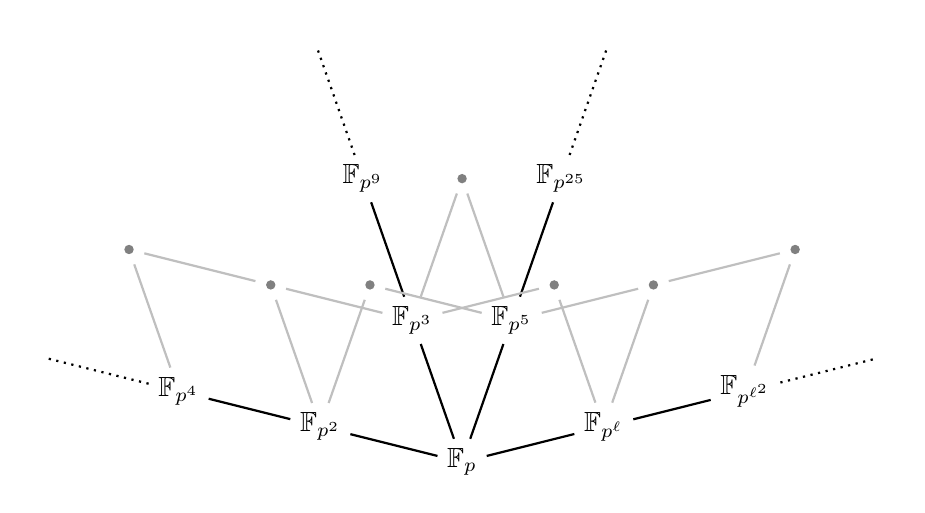
\begin{tikzpicture}[scale=.9]
    \coordinate (T2) at (-2, 0.5);
    \node (Fp) at (0, 0) {$\mathbb{F}_p$};
    \node (Fp2) at ($(Fp) + (T2)$) {$\mathbb{F}_{p^2}$};
    \node (Fp4) at ($(Fp2) + (T2)$) {$\mathbb{F}_{p^4}$};
    \node (Fp2l) at ($(Fp4) + (T2)$) {};% {$\FF_p^{(2)}$};
    % ---------------------
    \coordinate (T3) at (-0.7, 2);
    \node (Fp3) at ($(Fp) + (T3)$) {$\mathbb{F}_{p^3}$};
    \node (Fp9) at ($(Fp3) + (T3)$) {$\mathbb{F}_{p^9}$};
    \node (Fp3l) at ($(Fp9) + (T3)$) {};% {$\FF_p^{(3)}$};
    % ---------------------
    \coordinate (T5) at (0.7, 2);
    \node (Fp5) at ($(Fp) + (T5)$) {$\mathbb{F}_{p^5}$};
    \node (Fp25) at ($(Fp5) + (T5)$) {$\mathbb{F}_{p^{25}}$};
    \node (Fp5l) at ($(Fp25) + (T5)$) {};% {$\FF_p^{(5)}$};
    % ---------------------
    \coordinate (Tl) at (2, .5);
    \node (Fpl) at ($(Fp) + (Tl)$) {$\mathbb{F}_{p^\ell}$};
    \node (Fpl2) at ($(Fpl) + (Tl)$) {$\mathbb{F}_{p^{\ell^2}}$};
    \node (Fpll) at ($(Fpl2) + (Tl)$) {};% {$\FF_p^{(\ell)}$};
    % ---------------------
    \node[dotstyle] (dot1) at ($(Fp2) + (Fp3) - (Fp)$) {};
    \node[dotstyle] (dot2) at ($(Fp4) + (dot1) - (Fp2)$) {};
    \node[dotstyle] (dot3) at ($(Fp2) + (Fp5) - (Fp)$) {};
    \node[dotstyle] (dot4) at ($(Fp3) + (Fp5) - (Fp)$) {};
    \node[dotstyle] (dot5) at ($(Fp3) + (Fpl) - (Fp)$) {};
    \node[dotstyle] (dot6) at ($(Fp5) + (Fpl) - (Fp)$) {};
    \node[dotstyle] (dot7) at ($(Fpl2) + (dot6) - (Fpl)$) {};
    % ---------------------
    \draw
    (Fp)
    edge[edgetower] (Fp2)
    edge[edgetower] (Fp3)
    edge[edgetower] (Fp5)
    edge[edgetower] (Fpl)
    (Fp2)
    edge[edgetower] (Fp4)
    edge[edgecomp] (dot1)
    (Fp4)
    edge[edgetower, dotted] (Fp2l)
    edge[edgecomp] (dot2)
    (dot1)
    edge[edgecomp] (dot2)
    (Fp3)
    edge[edgetower] (Fp9)
    edge[edgecomp] (dot1)
    edge[edgecomp] (dot4)
    (Fp9)
    edge[edgetower, dotted] (Fp3l)
    (Fp5)
    edge[edgetower] (Fp25)
    edge[edgecomp] (dot4)
    edge[edgecomp] (dot6)
    (Fp25)
    edge[edgetower, dotted] (Fp5l)
    (Fpl)
    edge[edgetower] (Fpl2)
    edge[edgecomp] (dot6)
    (Fpl2)
    edge[edgetower, dotted] (Fpll)
    edge[edgecomp] (dot7)
    (dot3)
    edge[edgecomp] (Fp2)
    edge[edgecomp] (Fp5)
    (dot5)
    edge[edgecomp] (Fp3)
    edge[edgecomp] (Fpl)
    (dot6)
    edge[edgecomp] (dot7);
  \end{tikzpicture}
  \caption{Extensions of $\mathbb{F}_p$.}
  \label{fig:alg-closure}
\end{figure}

\clearpage
\section{The compatibility problem}
\label{sec:compatibility-problem}

Now that we know how to go from one finite field $\mathbb{F}_{p^a}$ to another
$\mathbb{F}_{p^b}$, with $p\in\mathbb{N}$ a prime number and
\[
  a\,|\,b
\]
two integers, we would like to manage more than two finite fields
simultaneously. In other words, given a family
\[
  \F=\left\{ \mathbb{F}_{p^{a}}\,|\,a\in E \right\}
\]
for $E$ a subset of $\mathbb{N}\setminus\left\{ 0 \right\}$,
we want to be able to compute an embedding
\[
  \mathbb{F}_{p^a}\emb\mathbb{F}_{p^b}
\]
each time that we have $\mathbb{F}_{p^a}, \mathbb{F}_{p^b}\in\F$ with $a$
dividing $b$, while maintaining \emph{compatibility} between all these
embeddings. From a pratical point of view, we want to build a computer algebra
system where the users can embed the field they are working with in a bigger
finite field, or conversely if an element is known to belong to a smaller field
than the ambient field, project it to a smaller field. In cryptology and coding
theory, finite fields are ubiquitus, and some algorithms require frequent change
of field. For example, in the
quasi-polynomial algorithm for discrete logarithm in small characteristic by
Granger, Kleinjung and Zumbrägel~\cite{GKZ14}, we have to work with a tower of
finite field extensions, and thus a computer algebra system automatically
dealing with the changes would be very convenient in order to implement their
algorithm. From a theoretical point of view, this leads to the question of the
arithmetic in the algebraic closure of some finite field $\mathbb{F}_p$
\[
  \bar{\mathbb{F}}_p=\bigcup_{j\in\mathbb{N}\setminus\left\{ 0
  \right\}}\mathbb{F}_{p^j}
\]
and its representation on a computer, a question that was for example
investigated in~\cite{DDS14}. 

If we \emph{just} want to compute embeddings between two finite
fields in $\F$ when it makes sense, we can use one of the algorithms presented
in Chapter~\ref{chap:isomorphism} each time we need it. In fact, we want to
build a data structure $\Lambda$ to represent all the extensions of
$\mathbb{F}_p$ that we need, and additional sub-goals might be desirable.
\begin{description}
\item[\emph{Effective embeddings:}] for any pair of extensions
  $k\subset K$ in $\Lambda$, there exists an efficiently computable
  embedding $\phi:k\to K$, and algorithms to evaluate $\phi$ on $k$,
  and the section $\phi^{-1}$ on $K$.
\item[\emph{Compatibility:}] the embeddings are \emph{compatible},
  \ie for any triple $k\subset K\subset L$ in $\Lambda$, and
  embeddings $\phi:k\to K$, $\psi:K\to L$, $\chi:k\to L$ such as shown in
  Figure~\ref{fig:compatibility}, one has
  $\chi=\psi\circ\phi$.
  \begin{figure}[h]
    \centering
    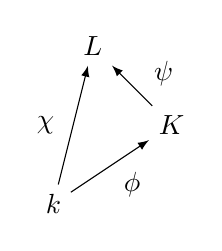
\begin{tikzpicture}
      \node (E) at (0, 0) {$k$};
      \node (F) at (1.5, 1) {$K$};
      \node (G) at (0.5, 2) {$L$};

      \draw[arrow] (E) -- (F);
      \draw[arrow] (E) -- (G);
      \draw[arrow] (F) -- (G);

      \node (f12) at (1, 0.25)
      {$\phi$};
      \node (f13) at (-0.1, 1)
      {$\chi$};
      \node (f23) at (1.4, 1.65)
      {$\psi$};
    \end{tikzpicture}

  \caption{Embeddings between finite fields $k\subset K\subset L$.}
  \label{fig:compatibility}
  \end{figure}
\item[\emph{Incrementality:}] the data associated with an extension
  (\eg its irreducible polynomial, change-of-basis matrices, \dots)
  must be computable efficiently and \emph{incrementally}, \ie 
  adding a new field extension to $\Lambda$ does not require
  recomputing data for all extensions already in $\Lambda$.
\item[\emph{Uniqueness:}] any extension of $\mathbb{F}_{p}$ is determined by an
  irreducible polynomial whose definition only depends on the
  characteristic $p$ and the degree of the extension.
\item[\emph{Generality:}] extensions of $\mathbb{F}_{p}$ can be represented by
  arbitrary irreducible polynomials.
\end{description}
We cannot fulfill all these conditions simultaneously, as
uniqueness and generality are in conflict with each other. One might prefer to
look for uniqueness or generality, depending on the situation, but it would
always be better to have effective embeddings, compatibility and incrementality.
In order to achieve the ``effective embeddings'' condition, we can use the
efficient algorithms presented in Chapter~\ref{chap:isomorphism}. The only
problem is that if we have three finite fields
\[
  k\subset K\subset L
\]
and three embeddings $\phi:k\to K$, $\psi:K\to L$, $\chi:k\to L$, there is no
guaranty that the diagram of Figure~\ref{fig:compatibility} commutes, \ie
\[
  \chi = \psi\circ\phi.
\]
If we want to achieve compatibility, we have to provide extra-work.
The two constructions presented in Sections~\ref{sec:conway}
and~\ref{sec:bosma-canon-steel} are both solutions oriented towards this goal.
Conway polynomials yield \emph{uniqueness} while the Bosma, Cannon and Steel
framework grants \emph{generality}.

\section{Conway polynomials}
\label{sec:conway}

% TODO
% ====
%
% Give a reference for the fact that Conway polynomials always exist?

Conway polynomials~\cite{Parker90, Scheerhorn92} are named after J. H. Conway,
they were introduced by Parker in 1990 and provide embeddings that are easy to
compute.

\begin{defi}[Conway polynomials]
  Let $p\in\mathbb{N}$ be a prime number. The $m$-th \emph{Conway polynomial}
  \[
    C_m\in\mathbb{F}_p[X]
  \]
  is the lexicographically smallest monic irreducible polynomial of degree $m$
  that is also primitive (\ie its roots generate $\mathbb{F}_{p^m}^\times$) and
  norm-compatible, \ie if
  \[
    m\,|\,n
  \]
  we have
  \[
    C_m(X^{\frac{p^n-1}{p^m-1}})\mod C_n = 0.
  \]
\end{defi}
The norm compatibility means that if one takes the norm relatively to the
extension 
\[
  \mathbb{F}_{p^n}/\mathbb{F}_{p^m}
\]
of a root of $C_n$, one obtains a root of $C_m$. This compatibility will allow
us to define compatible embeddings. Let $p\in\mathbb{N}$ be a prime number, $m,
n\in\mathbb{N}$ be two integers such that
\[
  m\,|\,n
\]
and let $C_m\in\mathbb{F}_{p}[X], C_n\in\mathbb{F}_{p}[Y]$ be the $m$-th and the $n$-th Conway
polynomial. Let 
\[
  k=\mathbb{F}_{p^m}=\mathbb{F}_p(\alpha_m)\cong\mathbb{F}_{p}[X]/(C_m)
\]
and
\[
  K = \mathbb{F}_{p^n}=\mathbb{F}_p(\alpha_n)\cong\mathbb{F}_{p}[Y]/(C_n)
\]
with $\alpha_m=\bar X\in k$ and $\alpha_n=\bar Y\in K$. Now, we define the
embedding
\[
\begin{array}{cccl}
  \embed{k}{K}:&k&\emb &K\\
  & \alpha_m&\mapsto&(\alpha_n)^{\frac{p^n-1}{p^m-1}}
\end{array}
\]
that sends $\alpha_m$ to $(\alpha_n)^{\frac{p^n-1}{p^m-1}}$, the norm of
$\alpha_n$ relative to $k$. Because this is a field morphism, it is implied that
every polynomial in $\alpha_m$ is sent to the same polynomial in
$(\alpha_m)^{\frac{p^n-1}{p^m-1}}$. That is indeed an embedding because of the
norm-compatibility condition in Conway polynomials. This definition also
provides compatibility thanks to the transitivity of the norm: let
\[
  k\subset K\subset L
\]
three finite fields defined using Conway polynomials, let
\[
  N_{K/k}, N_{L/K}, N_{L/k}
\]
be the respective norms of the extensions
\[
  K/k, L/K, L/k
\]
and
\[
  \embed{k}{K}, \embed{K}{L}, \embed{k}{L}
\]
the corresponding embeddings. Then, for any element $x\in L$, we have
\[
  N_{L/k}(x) = N_{K/k}(N_{L/K}(x)),
\]
and it follows, using the fact that $\embed{K}{L}$ and $N_{K/k}$ commute, that
\[
  \embed{k}{L}=\embed{K}{L}\circ\embed{k}{K}.
\]
Therefore, using Conway polynomials to define all finite field extensions allows
compatibility \emph{a priori}: adding a new extension in the lattice does not
require any computation and the form of the embedding is already known. The
only condition is to define each extension using the Conway polynomial of the
corresponding degree. These polynomials always exist so this is possible,
although the best known algorithm to compute Conway polynomials has exponential
complexity~\cite{HL98} in the degree of the polynomial. Because the cost of
computing Conway polynomials is
prohibitive, they are often precomputed and tabulated up to a certain degree in
many computer algebra systems. As a result, most computer algebra systems use
Conway polynomial to represent finite fields of small degrees, and switch to
other representations when Conway polynomials are no longer available. This
strategy leads to efficient lattices of compatibly embedded finite fields, at
least in small degrees, but at the cost of generality, because the finite fields
extensions cannot be user-defined and high degree extensions cannot be included
in the lattice. We see in Section~\ref{sec:bosma-canon-steel} that those issues
can be adressed by using another method 
defined by Bosma, Canon, and Steel~\cite{BCS97}, but the price to compute each
embedding is higher.
% TODO
% ====
%
% Say something about the evaluation of the embeddings coming from Conway
% polynomials

\section{The Bosma-Canon-Steel framework}
\label{sec:bosma-canon-steel}

In 1987, Bosma, Canon and Steel proposed a new framework~\cite{BCS97} to deal
with lattices of finite field extensions. These algorithms were initially
implemented in the computer algebra system MAGMA~\cite{Magma}. The framework allows the user
to define finite fields with custom polynomials, and compute the
correct embeddings on the fly, in a way that guarantees that at least one
compatible embedding will always exist between two finite fields, when that
makes sense. To the best of my knowledge, this framework was only used in MAGMA
until very recently. We first implemented the framework using Nemo and Flint and
presented our software in the symbolic computation conference ISSAC in
2018~\cite{DRR18}. In 2019, the code was also added to the official branch of
Nemo, and Nemo can now deal with finite field extensions and compatibly embed
them, in the case where the characteristic $p$ of the fields fits in a machine
word. There are no theretical obstacles preventing from implementing the
algorithm in arbitrarily large characteristic, but some tools were lacking at
the C level (\ie in Flint).

\subsection{The Bosma-Canon-Steel algorithm}
\label{sec:bcs-alg}
\paragraph{Notations and first results.} Let $p\in\mathbb{N}$ be a prime number
and $q$ a power of $p$. We present the results over the prime field
$\mathbb{F}_p$, but they can be extended to $\mathbb{F}_q$ without any new
difficulty. Given two finite fields $k$ and $K$ with cardinalities
\[
  \Card k = p^m
\]
and
\[
  \Card K =  p^n
\]
such that $m$ divides $n$, we know that $k$ can be embedded in $K$. In other
words, we know that $K$ contains one subfield
\[
  k'=\left\{ x\in K\,|\,x^{p^m}=x \right\}\subset K
\]
with 
\[
  \Card k' = p^m.
\]
There is exactly one subfield $k'$ in $K$ that has the same cardinality as $k$,
but there exist $m$ different ways to map $k$ to $k'$. One way of seeing that is
to say that an element $\alpha\in k$ generating $k$ has a minimal polynomial
$\pi$ over $\mathbb{F}_p$ of degree $m$, and that $\alpha$ can be mapped to any
one of the $m$ roots of $\pi$ in $K$. This choice sets the embedding because any
element in $k$ can be written as
\[
  \sum_{j=0}^{m-1}a_j \alpha^j,
\]
with $a_j\in\mathbb{F}_p$. We write $k\emb K$ if an explicit embedding has been
chosen. Let
\[
  k\subset K\subset L
\]
with $k\emb K$ and $k\emb L$, as in Figure~\ref{fig:incomplete}. The foundations
of the Bosma-Canon-Steel framework lay on the fact that we precisely know how many
compatible embeddings from $K$ to $L$ we can find.
\begin{figure}%[h]
  \centering
  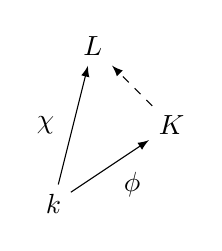
\begin{tikzpicture}
    \node (E) at (0, 0) {$k$};
    \node (F) at (1.5, 1) {$K$};
    \node (G) at (0.5, 2) {$L$};

    \draw[arrow] (E) -- (F);
    \draw[arrow] (E) -- (G);
    \draw[dashed-arrow] (F) -- (G);

    \node (f12) at (1, 0.25) {$\phi$};
    \node (f13) at (-0.1, 1) {$\chi$};
    %\node (f23) at (1.4, 1.65) {$\psi$};
  \end{tikzpicture}
\caption{Incomplete embedding diagram.}
\label{fig:incomplete}
\end{figure}
\begin{prop}[{\cite[Thm.~2.1]{BCS97}}]
  \label{prop:number-embeddings}
  Let $l\,|\,m\,|\,n$ be three integers and let
  \[
    k\subset K\subset L
  \]
  be three finite field extensions of $\mathbb{F}_p$, with respective
  cardinalities $p^l$, $p^m$ and $p^n$. If $k$ is embedded in $K$ and $L$,
  \ie if $k\emb K$ and $k\emb L$, then there are $m/l$ compatible embeddings
  from $K$ to $L$.
\end{prop}
\begin{proof}
  Let $\phi:k\to K$ be the embedding from $k$ to $K$ and $\chi:k\to L$ the
  embedding from $k$ to $L$. Let $\widetilde\psi:K\to L$ be any embedding from $K$ to
  $L$. The maps $\chi$ and $\widetilde\psi\circ\phi$ are two embeddings from
  $k$ to $L$.
  There are only $l$ such maps, because if $\alpha$ is a generating element in
  $k$ and if $\pi$ is its minimal polynomial over $\mathbb{F}_p$, then an
  embedding from $k$ to $L$ necessarily sends $\alpha\in k$ to a root $\beta\in
  L$ of $\pi$ in $L$.
  The embedding is then uniquely defined by 
  \[
    \alpha\mapsto\beta
  \]
  and there are $l$ such roots, that are all conjugates, thus we know that there
  exists
  \[
    \sigma\in\Gal(L/\mathbb{F}_p)
  \]
  such that
  \[
    \chi = \sigma\circ\widetilde\psi\circ\phi.
  \]
  If we set
  \[
    \psi=\sigma\circ\widetilde\psi,
  \]
  we obtain a compatible embedding $\psi:K\to L$ from $K$ to $L$. If we
  compose $\psi$ with a $\chi(k)$-automorphism of $L$, \ie an automorphism of
  $\psi(K)$ that
  fixes the subfield $\chi(k)$, we still obtain a compatible embedding because
  the images of the elements in $\chi(k)$ are unchanged. Now, we know that
  \[
    \Card\Gal(\psi(K)/\chi(k)) = m/l,
  \]
  thus we know that there are exactly $m/l$ embeddings from $K$ to $L$ that
  are compatible with $\phi$ and $\chi$.
\end{proof}
In the future, if we have two finite fields $k$ and $K$ such that $k\emb K$
with an explicit embedding $\phi:k\to K$, we will often identify $k$ with
its isomorphic image $\phi(k)\cong k$ in $K$, for the sake of simplicity. We
 also have a constructive version of Proposition~\ref{prop:number-embeddings}.
\begin{prop}[{\cite[Thm.~2.2]{BCS97}}]
  \label{prop:number-embeddings-constructive}
  Let $l\,|\,m\,|\,n$ be three integers and let
  \[
    k\subset K\subset L
  \]
  be three finite field extensions of $\mathbb{F}_p$, with respective
  cardinalities $p^l$, $p^m$ and $p^n$. Assume that $k\emb K$ and $k\emb L$,
  and let $\phi=\embed{k}{K}$, $\chi=\embed{k}{L}$ be the respective embeddings.
  Let also $\alpha\in K$ be an element that generates $K$ over $k$ and
  \[
    \pi_k=\Minpoly_k(\alpha)
  \]
  the minimum polynomial of $\alpha$ over $k$. Let $\rho\in L$ be a root of
  $\pi_k$ in $L$. Let $\psi:K\to L$ be the map defined by
  \[
    \psi\left(\sum_{j=0}^{m/l-1}x_j\alpha^j\right) = \sum_{j=0}^{m/l-1}x_j\rho^j,
  \]
  using the unique representation of any element of $K$ as $\sum_j x_j
  \alpha^j$ with $x_j\in k$. Then $\psi$ is an embedding from $K$ to $L$ that
  is compatible with $\phi$ and $\chi$, \ie we have
  \[
    \chi = \psi\circ\phi.
  \]
\end{prop}
\begin{proof}
  The root $\rho$ in $L$ exists since we know that $\pi_k$ has a root in $K$
  and $K\subset L$. The map $\psi$ is then well-defined because of the uniqueness of the
  representation of the elements in $K$ as $\sum_jx_j\alpha^j$. The elements
  $\alpha$ and $\rho$ have the same minimum polynomial so the map $\psi$ is a
  homomorphism. The map $\psi$ is also injective and thus it is an embedding
  from $K$ to $L$. The compatibility condition holds by construction.
\end{proof}
\begin{rem}
\label{rem:base-field}

In fact, in our implementation and even in
Proposition~\ref{prop:several-subfields}, this result will not be used as is and
we will usually take $\alpha\in K$ an element generating $K$ over the base
field $\mathbb{F}_p$ instead of over $k$. Indeed, if $\alpha$ generates $K$
over $\mathbb{F}_p$, it also generates $K$ over $k$. We can still take a root
$\rho$ of $\Minpoly_{k}(\alpha)$ because
\[
  \Minpoly_k(\alpha)\,|\,\Minpoly_{\mathbb{F}_p}(\alpha)
\]
and so a root of $\Minpoly_{k}(\alpha)$ is necessarily a root of
$\Minpoly_{\mathbb{F}_p}(\alpha)$. As a result, we can use the
$\mathbb{F}_p$-algebra structure of $K$ and still achieve compatibility with
the subfield $k$.
\end{rem}
Although the result of Proposition~\ref{prop:number-embeddings} captures only
one configuration among the three different possibilities of
Figure~\ref{fig:triangles}, it is the most important case. Indeed, if we
already know $\embed{k}{K}$ and $\embed{K}{L}$ (the configuration in the
middle of Figure~\ref{fig:triangles}), we can just set
\[
  \embed{k}{L} = \embed{K}{L}\circ\embed{k}{K}.
\]
Finally the configuration on the right, where we know $\embed{k}{L}$ and
$\embed{K}{L}$, is also irrelevant because, by construction, this case never
happens when working with the Bosma-Canon-Steel framework.
\begin{figure}
  \centering
  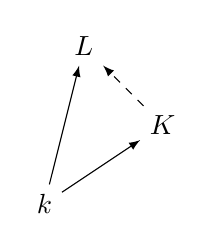
\begin{tikzpicture}
    \node (E) at (0, 0) {$k$};
    \node (F) at (1.5, 1) {$K$};
    \node (G) at (0.5, 2) {$L$};

    \draw[arrow] (E) -- (F);
    \draw[arrow] (E) -- (G);
    \draw[dashed-arrow] (F) -- (G);
  \end{tikzpicture}
  \phantom{and}
  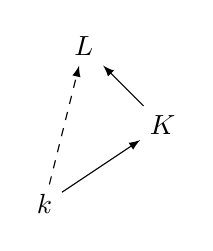
\begin{tikzpicture}
    \node (E) at (0, 0) {$k$};
    \node (F) at (1.5, 1) {$K$};
    \node (G) at (0.5, 2) {$L$};

    \draw[arrow] (E) -- (F);
    \draw[dashed-arrow] (E) -- (G);
    \draw[arrow] (F) -- (G);

  \end{tikzpicture}
  \phantom{and}
  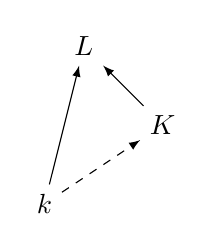
\begin{tikzpicture}
    \node (E) at (0, 0) {$k$};
    \node (F) at (1.5, 1) {$K$};
    \node (G) at (0.5, 2) {$L$};

    \draw[dashed-arrow] (E) -- (F);
    \draw[arrow] (E) -- (G);
    \draw[arrow] (F) -- (G);

  \end{tikzpicture}
  \caption{The different configurations with triangles.}
  \label{fig:triangles}
\end{figure}

\paragraph{Description of the framework.} The general strategy of Bosma, Canon,
and Steel to compute and maintain the data of several finite fields and
compatible embeddings between them is to ensure that some properties are
conserved at all times. If $k=\mathbb{F}_{p^m}$ is a finite extension of
$\mathbb{F}_p$, we define
\[
  \deg (k) = \left[ k:\mathbb{F}_p \right] = m
\]
the extension degree over $\mathbb{F}_p$.
\begin{defi}[Lattice of compatibly embedded finite fields]
  \label{defi:lattice-bcs}
  Let $q$ be a power of $p$ a prime number and $\mathbb{F}_p$ the finite field
  with $q$ elements. The pair
\[
  \Lambda = (\mathcal K, \Phi),
\]
where $\mathcal K$ is a collection of finite fields sharing the same base field
$\mathbb{F}_p$ and $\Phi$ is a collection of embeddings between members of
$\mathcal K$,
is called a \emph{lattice of compatibly embedded finite fields} if the following
conditions are satisfied:
\begin{description}
  \item[CE1 (unicity)] for each pair $(k, K)$ of elements in $\mathcal K$, there exists
    at most one corresponding embedding $\embed{k}{K}\in\Phi$.
    \item[CE2 (reflexivity)] For each $k\in \mathcal K$, the identity map
    $\Id_k=\embed{k}{k}$ is in $\Phi$.
  \item[CE3 (base subfield)] There is exactly one $k\in \mathcal K$ such that
    $\deg(k)=1$, and for all $K\in \mathcal K$, there exists $\embed{\mathbb{F}_p}{K}\in\Phi$.
  \item[CE4 (invertibility)] If $k\emb K$ and $\deg(k)=\deg(K)$, then $K\emb k$ and
    $\embed{K}{k}=\embed{k}{K}^{-1}$.
  \item[CE5 (transitivity)] For any triple $(k, K, L)$ of elements in $\mathcal
    K$, if $k\emb K\emb L$ then $k\emb L$ and
    $\embed{k}{L}=\embed{K}{L}\circ\embed{k}{K}$.
  \item[CE6 (intersections)] For each $k, K, L\in \mathcal K$ such that $K\emb L$ and
    $k\emb L$, there exists $I\in \mathcal K$ such that
    $\deg(I)=\gcd(\deg(k), \deg(K))$
    and $I\emb k$, $I\emb K$.
\end{description}
\end{defi}
Conditions CE1 to CE5 are quite natural, some of them are technical and
are not important in our implementation. For example, Condition~CE3
is totally free in our implementation because we work with $q=p$ and the
elements of our fields are represented by polynomials over
$\mathbb{F}_p=\mathbb{Z}/p\mathbb{Z}$, thus the subfield
$\mathbb{F}_p\subset\mathbb{F}_{p^m}$ is always represented by the constant
polynomials and the embedding is trivial. Nevertheless, Condition~CE6 is
important both from a theoretical and on an implementation point of view: it
ensures that the implicit embeddings between common subfields are made explicit,
in order to prevent any possible future incompatibility, and it forces the
computer algebra software to compute extra embeddings that the user might not
need. Assume that we have embedded $\mathbb{F}_{p^4}$ and $\mathbb{F}_{p^6}$
into $\mathbb{F}_{p^{12}}$, there is now an implicit isomorphism between the two
copies of the quadratic subfield $\mathbb{F}_{p^2}$ in $\mathbb{F}_{p^4}$ and
$\mathbb{F}_{p^6}$. Any future embedding from $\mathbb{F}_{p^4}$ of
$\mathbb{F}_{p^6}$ in an extension of
$\mathbb{F}_{p^{12}}$, say $\mathbb{F}_{p^{24}}$ for example, must now take into
account the isomorphism between the two quadratic fields. Condition CE6 ensures
that this implicit isomorphism is made explicit by adding a quadratic field
$\mathbb{F}_{p^2}$ in the lattice and explicitly embedding it in
$\mathbb{F}_{p^4}$ and $\mathbb{F}_{p^6}$, and by transitivity in
$\mathbb{F}_{p^{12}}$ and $\mathbb{F}_{p^{24}}$.
\begin{center}
      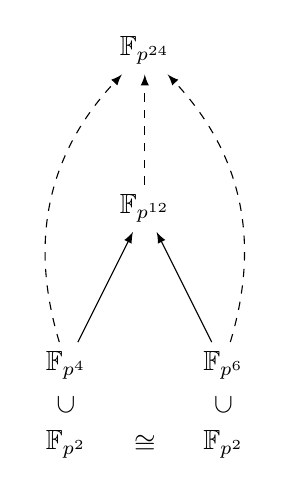
\begin{tikzpicture}
        \node (4) at (0, 0) {$\mathbb{F}_{p^{4}}$};
        \node (6) at (2, 0) {$\mathbb{F}_{p^{6}}$};
        \node (12) at (1, 2) {$\mathbb{F}_{p^{12}}$};
        \node (24) at (1, 4) {$\mathbb{F}_{p^{24}}$};

      \draw[arrow] (4) -- (12);
      \draw[arrow] (6) -- (12);

      \node[rotate=90] (sub1) at (0, -0.5) {$\subset$};
      \node[rotate=90] (sub2) at (2, -0.5) {$\subset$};
        \node (2) at (0, -1) {$\mathbb{F}_{p^{2}}$};
        \node (2bis) at (2, -1) {$\mathbb{F}_{p^{2}}$};
        \node (iso) at (1, -1) {$\cong$};
      \draw[dashed-arrow] (12) -- (24);
      \draw[dashed-arrow] (4) to[bend left] (24);
      \draw[dashed-arrow] (6) to[bend right] (24);
    \end{tikzpicture}
\end{center}
Under the conditions described in Definition~\ref{defi:lattice-bcs}, we
can add new embeddings in our lattice $\Lambda$ without compromising the
compatibility of the lattice. Assume that we want to embed $K$ into $L$. We have
seen that the relevant elements that restrict the number of compatible
embeddings are the common subfields of $K$ and $L$. If there is only one common
subfield $k$, we are in the case described by
Propositions~\ref{prop:number-embeddings}
and~\ref{prop:number-embeddings-constructive}. Now, assume that there are many
common subfields, like shown in Figure~\ref{fig:incomplete-sev}.% and let
%\[
%  C = \left\{ k\in\mathcal K\,|\,k\emb K\text{ and }k\emb L \right\}
%\]
%be the set of these common subfields.
\begin{figure}
  \centering
    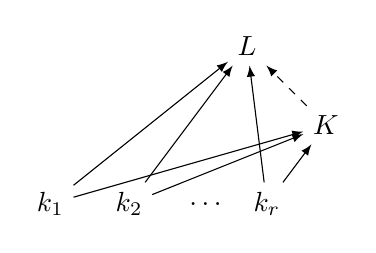
\begin{tikzpicture}
      \node (E1) at (-2, 0) {$k_1$};
      \node (E2) at (-1, 0) {$k_2$};
      \node (Er) at (0.75, 0) {$k_r$};
      \node (F) at (1.5, 1) {$K$};
      \node (G) at (0.5, 2) {$L$};
      \node (p) at (0, 0) {$\dots$};

      \draw[arrow] (E1) -- (F);
      \draw[arrow] (E1) -- (G);
      \draw[arrow] (E2) -- (F);
      \draw[arrow] (E2) -- (G);
      \draw[arrow] (Er) -- (F);
      \draw[arrow] (Er) -- (G);
      \draw[dashed-arrow] (F) -- (G);
  \end{tikzpicture}
  \caption{An incomplete diagram with several subfields.}
  \label{fig:incomplete-sev}
\end{figure}
In the same fashion as was done in Proposition~\ref{prop:number-embeddings}, we
can abtractly describe how many compatible embeddings exist (this is done
in~\cite[Section 2.5]{BCS97}), but we rather focus on the constructive part. In
some sense, this is just a generalization of
Proposition~\ref{prop:number-embeddings-constructive}, where we allow an
arbitrary number of common subfields.
\begin{prop}
  \label{prop:several-subfields}
  Let $K, L\in\mathcal K$ be two finite fields with
  \[
    K\subset L
  \]
  and let $k_1, \dots, k_r\in\mathcal K$ be the common subfields of $K$ and $L$,
  \ie for all $1\leq j\leq r$, we have
  \[
    k_j\emb K\text{ and }k_j\emb L.
  \]
  Let $\alpha\in K$ be an element generating $K$ over $\mathbb{F}_p$ and
  \[
    \pi = \gcd_{1\leq j\leq r}(\Minpoly_{k_j}(\alpha)).
  \]
  Let $\rho\in L$ be a root of $\pi$ in $L$ and let $\psi:K\to L$ be the map
  defined by
  \[
    \psi\left(\sum_{j=0}^{\deg(K)-1}x_j\alpha^j\right) =
    \sum_{j=0}^{\deg(K)-1}x_j\rho^j
  \]
  using the unique representation of elements in $K$ as $\sum_j x_j\alpha^j$
  with $x_j\in\mathbb{F}_p$. Then $\psi$ is an embedding from $K$ to $L$ that is
  compatible with all the embeddings $\embed{k_j}{K}$ and $\embed{k_j}{L}$.
\end{prop}
\begin{proof}
  Let $\alpha\in K$ be an element generating $K$ over the base field
  $\mathbb{F}_p$. Then, for all $1\leq j\leq r$, $\alpha$ also generates $K$
  over $k_j$. Now consider the polynomial
  \[
    \pi = \gcd_{1\leq j\leq r}(\Minpoly_{k_j}(\alpha)).
  \]
  For all $1\leq j\leq r$, we have by definition
  \[
    (\Minpoly_{k_j}(\alpha))(\alpha) = 0
  \]
  and so
  \[
    T-\alpha\,|\,\Minpoly_{k_j},
  \]
  thus the polynomial $T-\alpha\in K[T]$ also divides $\pi$, which consequently is not the constant
  polynomial $1$ and has a root in $K$. Since we have
  \[
    K\subset L,
  \]
  it follows that $\pi$ also has a root in $L$. Let $\rho\in L$ be a root of $\pi$
  in $L$, then for all $1\leq j\leq r$, $\rho$ is a root of
  the polynomial $\Minpoly_{k_j}(\alpha)$ and thus the map $\psi$ is an
  embedding that is compatible, by
  Proposition~\ref{prop:number-embeddings-constructive} and
  Remark~\ref{rem:base-field}, with the embeddings
  $\embed{k_j}{K}$ and $\embed{k_j}{L}$.
\end{proof}
\begin{rem}
  \label{rem:greatest-common-subfield}
  There is another way of describing the polynomial $\pi$ in
  Proposition~\ref{prop:several-subfields}. Let $K'\subset K$ be the
  subfield of $K$ generated by the fields $k_j\subset K$, in fact we have
  \[
    \pi = \Minpoly_{K'}(\alpha).
  \]
  Indeed, we have
  \begin{align*}
    \Gal(K/K') &= \left\{ \sigma\in\Gal(K/\mathbb{F}_p)\,|\,\forall x\in
  K',\,\sigma(x) = x \right\}\\
  &= \left\{ \sigma\in\Gal(K/\mathbb{F}_p)\,|\,\forall 1\leq j\leq r,\,\forall x\in
  k_j,\,\sigma(x) = x \right\}\\
  &= \bigcap_{1\leq j\leq r}\Gal(K/k_j),
  \end{align*}
  and thus it follows that
  \begin{align*}
    \Minpoly_{K'}(\alpha) &= \prod_{\sigma\in\Gal(K/K')}T-\sigma(\alpha)\\
    &=\prod_{\sigma\in\bigcap_{1\leq j\leq r}\Gal(K/k_j)}T-\sigma(\alpha)\\
    &= \gcd_{1\leq j\leq
    r}\left(\prod_{\sigma\in\Gal(K/k_j)}T-\sigma(\alpha)\right)\\
    &= \gcd_{1\leq j\leq r}(\Minpoly_{k_j}(\alpha)).
  \end{align*}
  where $T$ is the indeterminate. In fact, in~\cite{BCS97}, it is shown that
  there is exactly one compatible ismorphism between $K'$ and $L'$, the subfield
  of $L$ generated by the subfields $k_j$ in $L$, and that there are
  \[
    \deg(K)/\deg(K'),
  \]
  which is the degree of $\pi$, different compatible embeddings from $K$ to $L$.
\end{rem}

\subsection{Implementation in Nemo}
\label{sec:bcs-implem}

Although Proposition~\ref{prop:number-embeddings} suggests to compute a random
embedding and then to ``correct'' it, we follow the method of
Propositions~\ref{prop:number-embeddings-constructive} and~\ref{prop:several-subfields} and
we directly compute compatible embeddings using the naive algorithm, that relies
on polynomial factorization. The whole framework is implemented in
Nemo~\cite{Nemo} since Fall $2019$, at least for finite fields with
word-sized characteristic, \ie finite fields extensions
\[
  \mathbb{F}_{p^m}
\]
where $p$ is a prime number that fits in $64$ bits. The source code is available
in Nemo's github repository\footnote{\url{https://github.com/Nemocas/Nemo.jl}}.
Almost all of the code is directly written in the Julia library Nemo, because it
consists mostly of high level manipulations, but the critical routines, such as
factorization, are implemented in the C library Flint and are called from Nemo.

\paragraph{Types and data structures.} There are two types of finite fields in Nemo/Flint,
those with a word-sized characteristic and those with arbitrarily large
characteristic. The former have the type \texttt{fq\_nmod\_ctx\_t} in Flint and
\texttt{FqNmodFiniteField} in Nemo, while the field elements have the type
\texttt{fq\_nmod\_t} in Flint and \texttt{fq\_nmod} in Nemo. The corresponding
types in arbitrarily large characteristic are \texttt{fq\_ctx\_t},
\texttt{FqFiniteField}, \texttt{fq\_t} and
\texttt{fq}. We may use a Flint name for a type in Nemo or vice versa, because
the types represent the same things: Nemo being a wrapper of Flint in this case.
The main difference between the two types is that the polynomials representing the
elements of these fields have different types, depending on whether they have
arbitrarily large coefficients (\texttt{fmpz\_mod\_poly\_t}) or if their
coefficients fit in a $64$ bit word (\texttt{nmod\_poly\_t}). Since the
representation of the elements varies, so do the algorithms for manipulating
various elements in Flint (matrices, polynomials) with word-sized or arbitrarily
large coefficients. Some of the algorithms implemented for matrices with
word-sized coefficients are not implemented for arbitrarily large coefficient and
as a consequence we were only able to implement the Bosma-Canon-Steel algorithm
for the type \texttt{FqNmodFiniteField}. This type contains
\begin{itemize}
  \item the characteristic $p$ (that fits in $64$ bits);
  \item the irreducible polynomial used to define the field (of type
    \texttt{nmod\_poly\_t});
  \item various technical precomputations that are stored for performance;
  \item two dictionaries containing information about the lattice of
    compatible embeddings.
\end{itemize}
Let $K$ be some finite field represented by the type \texttt{FqNmodFiniteField},
the two dictionaries stored in the data structure representing $K$ are called
\texttt{subfields} and \texttt{overfields}. They both map integers to lists of
embeddings. If the \texttt{subfields} dictionary has a key \texttt{l}, then the
associated value \texttt{subfields[l]} is a list of embeddings
\[
  \phi_j: k_j\to K
\]
where all the $k_j$ are finite fields of the corresponding degree
\texttt{l}. Note that this is a \emph{list}, because there might be several
different finite fields of the same degree embedded in $K$. Similarly, if the
\texttt{overfields} dictionary has a key \texttt{m}, then the corresponding
value \texttt{overfield[m]} is a list of embeddings
\[
  \psi_j:K\to L_j
\]
where all the $L_j$ are finite fields of degree \texttt{m}. Finally, the
embeddings $\phi:K\to L$ are represented by the type \texttt{FinFieldMorphism}, that
essentially contains information about the domain $K$, the codomain $L$,
the function $\phi$ and the preimage function $\phi^{-1}$.

\paragraph{General strategy.} The essential idea is to maintain a lattice of
compatibly embedded finite fields, \ie ensure that the conditions described in
Definition~\ref{defi:lattice-bcs} are met, at all
times. To do so, each time the user asks for a new embedding
\[
  \phi:K\to L,
\]
we must go through $3$ steps:
\begin{enumerate}
  \item for each subfield 
    \[
      M\subset L
    \]
    of $L$, check that the finite field $M\cap K$ is 
    embedded in $M$ and $K$, and if not, embed it. If there is not
    any finite field of degree 
    \[
      d=\gcd(\deg(M), \deg (K)),
  \]
    compute an
    arbitrary finite field $I$ of degree $d$ using Flint
    and embed $I$ in $M$ and $K$.
    \begin{center}
      \begin{tikzpicture}
        \node (K) at (0, 2) {$K$};
        \node (L) at (2, 4) {$L$};
        \node (M) at (4, 2) {$M$};
        \node (I) at (2, 0) {$K\cap M$};

        \draw[dashed-arrow] (K) to (L);
        \draw[arrow] (M) to (L);
        \draw[possible-arrow] (I) to (K);
        \draw[possible-arrow] (I) to (M);

        \node (?) at (1, 1) {\textbf{?}};
        \node (??) at (3, 1) {\textbf{?}};
      \end{tikzpicture}
    \end{center}
    This step ensures that Condition~CE6 on the
    \emph{intersections} holds. It is important to begin with this step, so
    that every implicit isomorphism between the different common subfields are
    made explicit and that the compatibility conditions concerning the
    embedding $K\emb L$ include them.
  \item Embed $K$ in $L$ using the procedure described in
    Proposition~\ref{prop:several-subfields}.
  \item Compute the ``transitive closure'' of the lattice, \ie compute the
    embeddings such that Condition~CE5 on \emph{transitivity} holds. 
\end{enumerate}
The first step might contain a recursive call to the embedding algorithm, thus
one might have to compute many additional embeddings behind the scenes in order
to have only one new embedding. 
% TODO
% ====
%
% Better understanding of ``many''. Quadratic? Proof? Example?

\paragraph{Main algorithms.} The embedding algorithm, called \texttt{embed}, thus follows the steps
described in the general strategy, alongside trivial verifications such as
checking if the embedding makes sense, checking if an embedding already exists,
and so on. There are three main algorithms, \texttt{intersections},
\texttt{find\_morphism} and \texttt{transitive\_closure}, each one respectively
corresponding to the first, the second, and the third step. In the first step,
we loop through all the subfields $M$ embedded in $L$ and we check that the
intersection $I = K\cap M$ is also embedded in $K$ and $M$. Different cases can
occur, depending on the relative position of $K$ and $M$ in the lattice of
finite fields, as described in Figure~\ref{fig:relative-positions}. If $I=K$
(case of the left side of Figure~\ref{fig:relative-positions}), then we only
need to check that $K$ is embedded in $M$. When
this is done, we do not need to compute anything else because the embedding from
$K$ to $L$ is then obtained via transitive closure. If $I=M$ (case in the
middle), then we need to check that $M$ is embedded in $K$. If $I$ is neither
$K$ or $L$ (case on the right side), then we first check if $I$ already exists
in the lattice of compatibly embedded finite fields, we create it if necessary,
and we finally check that it is embedded in both $K$ and $L$. In order
to know whether further computations are needed in the \texttt{embed}
algorithm, we return a boolean that is \texttt{false} if the encountered case
was the one where $I=K$. The \texttt{intersection} algorithm is also explained
in Algorithm~\ref{algo:intersections}. In Algorithm~\ref{algo:find-morphism},
called \texttt{find\_morphism}, we follow the method of
Proposition~\ref{prop:several-subfields} in order to find a compatible
embedding. If there are no particular conditions to meet, we just use polynomial
factorization to obtain an embedding, \ie we use the naive embedding algorithm.
When a suitable embedding $\phi:K\emb L$ has been found, in order to ensure that
the lattice $\Lambda$ is transitive, we apply
Algorithm~\ref{algo:transitive-closure} that loops through all subfields $k$ of
$K$, and letting $\psi:k\emb K$ be an embedding into $K$, checks that the
embedding $\phi\circ\psi$ is
also in the lattice. We then recursively call the \texttt{transitive\_closure}
procedure on the fields that $L$ is embedded into.
\begin{figure}
  \centering
  \begin{tikzpicture}
    \node (k) at (0, 0) {$K=I=K\cap M$};
    \node (M) at (0, 2) {$M$};
    \node (K) at (0, 4) {$L$};

    \draw[dashed-arrow] (k) to[bend right] (K);
    \draw[arrow] (M) to (K);
    \draw[possible-arrow] (k) to (M);
    \node (?) at (0, 1) {\textbf{?}};
  \end{tikzpicture}
  \quad
  \quad
  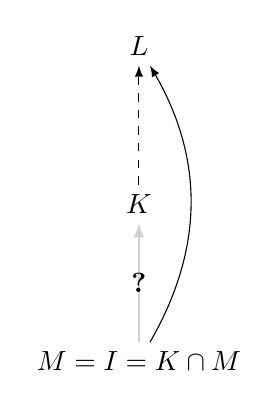
\begin{tikzpicture}
    \node (k) at (0, 2) {$K$};
    \node (M) at (0, 0) {$M=I=K\cap M$};
    \node (K) at (0, 4) {$L$};

    \draw[dashed-arrow] (k) to (K);
    \draw[arrow] (M) to[bend right] (K);
    \draw[possible-arrow] (M) to (k);
    \node (?) at (0, 1) {\textbf{?}};
  \end{tikzpicture}
  \quad
  \quad
  \begin{tikzpicture}
    \node (k) at (0, 2) {$K$};
    \node (K) at (2, 4) {$L$};
    \node (M) at (4, 2) {$M$};
    \node (I) at (2, 0) {$K\cap M$};

    \draw[dashed-arrow] (k) to (K);
    \draw[arrow] (M) to (K);
    \draw[possible-arrow] (I) to (k);
    \draw[possible-arrow] (I) to (M);

    \node (?) at (1, 1) {\textbf{?}};
    \node (??) at (3, 1) {\textbf{?}};
  \end{tikzpicture}
  \caption{Three different configurations when computing the intersection step
  of the Bosma-Canon-Steel framework.}
  \label{fig:relative-positions}
\end{figure}

\begin{algorithm}
  \caption{\texttt{intersections}}
  \label{algo:intersections}
  \begin{algorithmic}[1]
    \Require{$K$ and $L$ two finite fields of a lattice of compatibly embedded
    finite fields $(\mathcal K, \Phi)$}
    \Ensure{A boolean $b$ being \False if and only if no additional work is
  required}
  \State $b\gets\True$
  \ForAll{$M\emb L$}
  \State $d\gets\gcd({\left[ K:\mathbb{F}_p \right], \left[ M:\mathbb{F}_p
  \right]})$
  \If{$d=\left[ K:\mathbb{F}_p \right]$}
  \State $b\gets\False$\Comment{We obtain the final embedding by transitive
  closure}
  \State \texttt{embed}$(K, M)$
  \ElsIf{$d=\left[ M:\mathbb{F}_p \right]$}
  \State \texttt{embed}$(M, K)$
  \ElsIf{$I\cong\mathbb{F}_{p^d}\emb K$}\Comment{$\mathbb{F}_{p^{d}}$ already
exists in the computer algebra system}
  \State \texttt{embed}$(I, M)$
  \ElsIf{$I\cong\mathbb{F}_{p^d}\emb L$}\Comment{$\mathbb{F}_{p^{d}}$ already
exists in the computer algebra system}
  \State \texttt{embed}$(I, K)$
  \State \texttt{embed}$(I, M)$
  \Else
  \State $I\gets\mathbb{F}_{p^{d}}$\Comment{We create the field
    $\mathbb{F}_{p^{d}}$ in the computer algebra system}
  \State \texttt{embed}$(I, K)$
  \State \texttt{embed}$(I, M)$
  \EndIf
  \EndFor
  \State \Return{$b$}
  \end{algorithmic}
\end{algorithm}

\begin{algorithm}
  \caption{\texttt{find\_morphism}}
  \label{algo:find-morphism}
  \begin{algorithmic}[1]
    \Require{$K$ and $L$ two finite fields of a lattice of compatibly embedded
    finite fields $(\mathcal K, \Phi)$}
    \Ensure{$\phi:K\to L$ a compatible embedding}
    \State $C\gets\left\{k\in\mathcal K\,|\,k\emb K\text{ and }k\emb L \right\}$
    \State $\pi\gets\gcd_{k\in C}(\Minpoly_k(\alpha))$\Comment{$\alpha$ is a
      generator of $K$ over $\mathbb{F}_p$, the minimum polynomial is obtained
    via the Berlekamp-Massey algorithm.}
    \State $\rho\gets$ any root of $\pi$
    \State \Return{$\phi:K\to L,\,\alpha\mapsto\rho$}
  \end{algorithmic}
\end{algorithm}

\begin{algorithm}
  \caption{\texttt{transitive\_closure}}
  \label{algo:transitive-closure}
  \begin{algorithmic}[1]
    \Require{$\phi:K\emb L$ an embedding between two finite fields}
    \Ensure{ensures that the lattice of compatibly embedded finite fields
    $(\mathcal K, \Phi)$ is transitive}
    \ForAll{$\psi:k\emb K$}
    \State $\Phi\gets\Phi\cup\left\{ \phi\circ\psi \right\}$
    \EndFor
    \State $C\gets\left\{ M\in\mathcal K\mid L\emb M \right\}$
    \ForAll{$M\in C$}
    \State $\theta\gets (L\emb M)$
    \State \texttt{transitive\_closure}$(\theta)$
    \EndFor
  \end{algorithmic}
\end{algorithm}

\paragraph{Experimental results.}

All the tests in this section were performed on an Intel Core i7-7500U CPU
clocked at 2.70GHz, using Nemo 0.19.1 running on Julia 1.5.3, and
Nemo’s corresponding version of Flint. The benchmark functions are available in the
file \texttt{bencharks.jl} of the repository of the
thesis\footnote{\url{https://github.com/erou/thesis/.}}, as well as the data
that was used to plot the timings. All plots were made using gnuplot version 5.2
patchlevel 8, and the gnuplot files can also be found in the repository. Because
of how the Bosma-Canon-Steel framework works, in particular because of the
condition on the intersections, the time needed to compute a specific embedding
\[
  \mathbb{F}_{p^{m}}\emb\mathbb{F}_{p^{n}}
\]
heavily depends on the other embeddings in the lattice. Indeed, if there are no
embeddings in the lattice, the embedding computation is in that case essentially
the same as the factorization of a degree $m$ polynomial in
$\mathbb{F}_{p^{n}}[X]$. On the contrary, if a subfield
$\mathbb{F}_{p^{d}}$ of degree $d\mid m$ exists in the lattice (see
Figure~\ref{fig:illustration-common-subfield} for an illustration) and is embedded
in both $\mathbb{F}_{p^{m}}$ and $\mathbb{F}_{p^{n}}$, then the degree of the
polynomial that is factorized is at most $\frac{m}{d}$, and could be less if
several subfields exist, as explained in
Proposition~\ref{prop:several-subfields} and
Remark~\ref{rem:greatest-common-subfield}.
\begin{figure}[h]
  \label{fig:illustration-common-subfield}
  \centering
  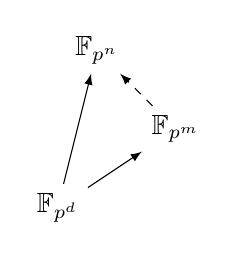
\begin{tikzpicture}
    \node (d) at (0, 0) {$\mathbb{F}_{p^{d}}$};
    \node (m) at (1.5, 1) {$\mathbb{F}_{p^{m}}$};
    \node (n) at (0.5, 2) {$\mathbb{F}_{p^{n}}$};

    \draw[dashed-arrow] (m) to (n);
    \draw[arrow] (d) to (m);
    \draw[arrow] (d) to (n);
  \end{tikzpicture}
  \caption{The computation of an embedding with a common subfield, that leads to
  the factorization of a polynomial of degree at most $m/d$.}
\end{figure}
As an illustration of that phenomenon, note that if the finite fields
$\mathbb{F}_{p^{2}}$, $\mathbb{F}_{p^{3}}$, $\mathbb{F}_{p^{6}}$ and
$\mathbb{F}_{p^{12}}$ are in our lattice, and if the embeddings
\[
  \mathbb{F}_{p^{2}}\emb \mathbb{F}_{p^{12}}
\]
and
\[
  \mathbb{F}_{p^{3}}\emb \mathbb{F}_{p^{12}}
\]
are already computed, then there is only one compatible embedding from
$\mathbb{F}_{p^{6}}$ to $\mathbb{F}_{p^{12}}$.
\begin{figure}[h]
  \centering
  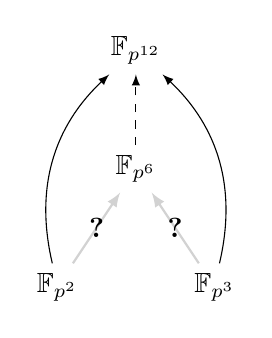
\begin{tikzpicture}
    \node (2) at (-1, 0) {$\mathbb{F}_{p^{2}}$};
    \node (3) at (1, 0) {$\mathbb{F}_{p^{3}}$};
    \node (6) at (0, 1.5) {$\mathbb{F}_{p^{6}}$};
    \node (12) at (0, 3) {$\mathbb{F}_{p^{12}}$};

    \draw[dashed-arrow] (6) to (12);
    \draw[arrow] (2) to[bend left] (12);
    \draw[arrow] (3) to[bend right] (12);
    \draw[possible-arrow] (2) to (6);
    \draw[possible-arrow] (3) to (6);
    \node (?) at (-0.5, 0.75) {\textbf{?}};
    \node (??) at (0.5, 0.75) {\textbf{?}};
  \end{tikzpicture}
  \caption{A lattice with four finite fields of size $p^2, p^3, p^6,
    p^{12}$ with some embeddings already computed.}
  \label{fig:example-F12}
\end{figure}
In this case, factorization in $\mathbb{F}_{p^{12}}[X]$ is not required, and the
work is essentially already done, although the embeddings from
$\mathbb{F}_{p^{2}}$ and $\mathbb{F}_{p^{3}}$ in $\mathbb{F}_{p^{6}}$ (easier
to compute) have to be computed if they are not already (see
Figure~\ref{fig:example-F12}).
In fact, when computing the embedding
\[
  \mathbb{F}_{p^{m}}\emb\mathbb{F}_{p^{n}},
\]
one of the decisive parameters is the degree of the extension 
\[
  \mathbb{F}_{p^{m}}/(L\cap\mathbb{F}_{p^{m}}),
\]
where $L$ is the finite field generated by the subfields already embedded in
$\mathbb{F}_{p^{n}}$. This measures both the freedom that we have to choose the
embedding $\mathbb{F}_{p^{m}}\emb\mathbb{F}_{p^{n}}$ and how much we already
know about it. If
\[
  \left[ \mathbb{F}_{p^{m}}:(L\cap\mathbb{F}_{p^{m}})\right]=1,
\]
then $\mathbb{F}_{p^{m}}$ is essentially already embedded in
$\mathbb{F}_{p^{n}}$ and there is only one compatible embedding. On the
contrary, if 
\[
  \left[ \mathbb{F}_{p^{m}}:(L\cap\mathbb{F}_{p^{m}})\right]=m,
\]
\ie if $L\cap\mathbb{F}_{p^{m}}=\mathbb{F}_p$, then there is absolutely no
compatibility condition to meet and we can take any embedding we want, but at
the same time we do not have any information about the embedding
$\mathbb{F}_{p^{m}}\emb\mathbb{F}_{p^{n}}$. We call this parameter the
\emph{defect} of the embedding $\mathbb{F}_{p^{m}}\emb\mathbb{F}_{p^{n}}$.
The defect depends on the state of the lattice $\Lambda$ at the moment of the
computation and has an important impact on the timings.
Consequently, there are several reasonable ways of measuring the timings
of the Bosma-Canon-Steel framework, which produce quite different results.
There is no major difference between two choices of characteristic $p$ so we
arbitrarily chose $p=3$. We
computed all the possible embeddings between finite fields of degree up to $400$
in two different ways. The first one consists in looping through the degrees
while increasing them, \ie for all $1\leq m\leq200$ and $m+1 \leq n\leq 400$, we
compute the embedding 
\[
  \mathbb{F}_{p^{m}}\emb \mathbb{F}_{p^{n}}
\]
whenever that makes sense, starting with $m=1, n=2$, then $m=1, n=3$, and so on, so
that the last embedding we compute is 
\[
  \mathbb{F}_{p^{200}}\emb\mathbb{F}_{p^{400}}.
\]
The second way consists in looping through the
degrees while decreasing them, \ie starting with
$\mathbb{F}_{p^{200}}\emb\mathbb{F}_{p^{400}}$, then
$\mathbb{F}_{p^{199}}\emb\mathbb{F}_{p^{398}}$ and so on until
$\mathbb{F}_{p}\emb\mathbb{F}_{p^{2}}$. Again, these two methods produce
different timing results because at the moment an embedding is computed, the
state of the lattice if not the same in the two cases. For example, the
embedding $\mathbb{F}_{p^{200}}\emb\mathbb{F}_{p^{400}}$ takes $3.5$ seconds to
be computed in the first test, while it takes $47.5$ seconds in the second one.
In Figure~\ref{fig:bcs-embed-from-2-up}, we plot the time needed to compute
embeddings of the form
\[
  \mathbb{F}_{p^{2}}\emb \mathbb{F}_{p^{m}}
\]
for $m\leq 400$ with the first method, \ie increasing degrees. In this case,
there are no common subfields when the embeddings are computed, thus the defect
is always $1$ and the naive embedding algorithm is applied.
\begin{figure}
  \centering
  \includegraphics{benchmarks/lattice-bcs/embed-from-2-up-3.eps}
  \caption{Timings for the computation of embeddings from $\mathbb{F}_{p^{2}}$
  to $\mathbb{F}_{p^{m}}$ for $m\leq 400$ and $2\mid m$, with $p=3$. The
  embeddings were computed with increasing degrees.}
  \label{fig:bcs-embed-from-2-up}
\end{figure}
When the embeddings are computed with decreasing degrees, there are a lot more
embeddings already in the lattice, thus the defect can be either $1$ or $2$. We
observe that the time needed to compute the embeddings is completely different
in those two cases, thus we use a logarithmic scale to emphasize the difference.
\begin{figure}
  \centering
  \includegraphics{benchmarks/lattice-bcs/embed-from-2-down-3.eps}
  \caption{Timings (logarithmic scale) for the computation of embeddings from
    $\mathbb{F}_{p^{2}}$ to $\mathbb{F}_{p^{m}}$ for $m\leq 400$ and $2\mid m$,
  with $p=3$. The embeddings were computed with decreasing degrees.}
  \label{fig:bcs-embed-from-2-down}
\end{figure}
The difference between the two methods is also noticeable when looking at the
embeddings to a fixed finite field. We look at the embeddings to the finite
fields of degree $360$ because it is a highly composite number, having $24$
different divisors: $1, 2, 3, 4, 5, 6, 8, 9, 10, 12, 15, 18, 20, 24, 30, 36, 40,
45, 60, 72, 90, 120, 180$ and $360$. In the first experiment, with increasing
degrees, all embeddings are computed in under one second, as shown in
Figure~\ref{fig:bcs-embed-to-360-up}. This is understandable because the defect is
never very high. In the second experiment, shown in
Figure~\ref{fig:bcs-embed-to-360-down}, the timing to compute the embedding 
\[
  \mathbb{F}_{p^{180}}\emb\mathbb{F}_{p^{360}}
\]
is approximately $30$ seconds, with a defect of $180$ because
$\mathbb{F}_{p^{360}}$ has no embedded subfields yet. After this computation,
only the embedding $\mathbb{F}_{p^{120}}\emb\mathbb{F}_{p^{360}}$ has a defect
equal to $2$ and all the others have a defect equal to $1$. This leads to very
fast computation for some embeddings, that are essentially already computed.
\begin{figure}
  \centering
  \includegraphics{benchmarks/lattice-bcs/embed-to-360-up-3.eps}
  \caption{Timings for the computation of embeddings from $\mathbb{F}_{p^{m}}$
  to $\mathbb{F}_{p^{360}}$ for $m\mid 360$, with $p=3$. The
  embeddings were computed with increasing degrees. We use logarithmic scales on
  both axes for readability.}
  \label{fig:bcs-embed-to-360-up}
\end{figure}
\begin{figure}
  \centering
  \includegraphics{benchmarks/lattice-bcs/embed-to-360-down-3.eps}
  \caption{Timings for the computation of embeddings from $\mathbb{F}_{p^{m}}$
  to $\mathbb{F}_{p^{360}}$ for $m\mid 360$, with $p=3$. The
  embeddings were computed with decreasing degrees. We use logarithmic scales on
  both axes for readability.}
  \label{fig:bcs-embed-to-360-down}
\end{figure}
When computing embeddings corresponding to extension of a fixed degree, \eg
extensions of type
\[
  \mathbb{F}_{p^{2m}}/\mathbb{F}_{p^{m}},
\]
the difference is also noteworthy: when the embeddings are computed with the
degrees decreasing (Figure~\ref{fig:bcs-embed-fixed-degree-down}), then the defect is
always maximum, thus the timings are rather smooth, while the computations with
the increasing degrees (Figure~\ref{fig:bcs-embed-fixed-degree-up}) produce
erratic timings because low defects lead to a huge speedup.
\begin{figure}
  \centering
  \includegraphics{benchmarks/lattice-bcs/embed-fixed-degree-from-12-to-24-up.eps}
  \caption{Timings (logarithmic scale) for the computation of embeddings from $\mathbb{F}_{p^{m}}$
  to $\mathbb{F}_{p^{2m}}$ for $1\leq m\leq 200$, with $p=3$. The
  embeddings were computed with increasing degrees.}
  \label{fig:bcs-embed-fixed-degree-up}
\end{figure}
\begin{figure}
  \centering
  \includegraphics{benchmarks/lattice-bcs/embed-fixed-degree-from-12-to-24-down.eps}
  \caption{Timings (logarithmic scale) for the computation of embeddings from $\mathbb{F}_{p^{m}}$
  to $\mathbb{F}_{p^{2m}}$ for $1\leq m\leq 200$, with $p=3$. The
  embeddings were computed with decreasing degrees.}
  \label{fig:bcs-embed-fixed-degree-down}
\end{figure}
In order to show the impact on the characteristic $p$ on the timings, we also
plot the time needed to compute the embedding
\[
  \mathbb{F}_{p^{12}}\emb\mathbb{F}_{p^{24}}
\]
for different primes $p$. Because the impact on the timing is logarithmic in the
characteristic $p$, we use each prime number found immediately after $2^j$,
for $1\leq j\leq m$, \ie $p\approx 2^j$. The result is shown in
Figure~\ref{fig:bcs-embed-primes}.
\begin{figure}
  \centering
  % GNUPLOT: LaTeX picture with Postscript
\begingroup
  \fontfamily{Times}%
  \selectfont
  \makeatletter
  \providecommand\color[2][]{%
    \GenericError{(gnuplot) \space\space\space\@spaces}{%
      Package color not loaded in conjunction with
      terminal option `colourtext'%
    }{See the gnuplot documentation for explanation.%
    }{Either use 'blacktext' in gnuplot or load the package
      color.sty in LaTeX.}%
    \renewcommand\color[2][]{}%
  }%
  \providecommand\includegraphics[2][]{%
    \GenericError{(gnuplot) \space\space\space\@spaces}{%
      Package graphicx or graphics not loaded%
    }{See the gnuplot documentation for explanation.%
    }{The gnuplot epslatex terminal needs graphicx.sty or graphics.sty.}%
    \renewcommand\includegraphics[2][]{}%
  }%
  \providecommand\rotatebox[2]{#2}%
  \@ifundefined{ifGPcolor}{%
    \newif\ifGPcolor
    \GPcolortrue
  }{}%
  \@ifundefined{ifGPblacktext}{%
    \newif\ifGPblacktext
    \GPblacktexttrue
  }{}%
  % define a \g@addto@macro without @ in the name:
  \let\gplgaddtomacro\g@addto@macro
  % define empty templates for all commands taking text:
  \gdef\gplbacktext{}%
  \gdef\gplfronttext{}%
  \makeatother
  \ifGPblacktext
    % no textcolor at all
    \def\colorrgb#1{}%
    \def\colorgray#1{}%
  \else
    % gray or color?
    \ifGPcolor
      \def\colorrgb#1{\color[rgb]{#1}}%
      \def\colorgray#1{\color[gray]{#1}}%
      \expandafter\def\csname LTw\endcsname{\color{white}}%
      \expandafter\def\csname LTb\endcsname{\color{black}}%
      \expandafter\def\csname LTa\endcsname{\color{black}}%
      \expandafter\def\csname LT0\endcsname{\color[rgb]{1,0,0}}%
      \expandafter\def\csname LT1\endcsname{\color[rgb]{0,1,0}}%
      \expandafter\def\csname LT2\endcsname{\color[rgb]{0,0,1}}%
      \expandafter\def\csname LT3\endcsname{\color[rgb]{1,0,1}}%
      \expandafter\def\csname LT4\endcsname{\color[rgb]{0,1,1}}%
      \expandafter\def\csname LT5\endcsname{\color[rgb]{1,1,0}}%
      \expandafter\def\csname LT6\endcsname{\color[rgb]{0,0,0}}%
      \expandafter\def\csname LT7\endcsname{\color[rgb]{1,0.3,0}}%
      \expandafter\def\csname LT8\endcsname{\color[rgb]{0.5,0.5,0.5}}%
    \else
      % gray
      \def\colorrgb#1{\color{black}}%
      \def\colorgray#1{\color[gray]{#1}}%
      \expandafter\def\csname LTw\endcsname{\color{white}}%
      \expandafter\def\csname LTb\endcsname{\color{black}}%
      \expandafter\def\csname LTa\endcsname{\color{black}}%
      \expandafter\def\csname LT0\endcsname{\color{black}}%
      \expandafter\def\csname LT1\endcsname{\color{black}}%
      \expandafter\def\csname LT2\endcsname{\color{black}}%
      \expandafter\def\csname LT3\endcsname{\color{black}}%
      \expandafter\def\csname LT4\endcsname{\color{black}}%
      \expandafter\def\csname LT5\endcsname{\color{black}}%
      \expandafter\def\csname LT6\endcsname{\color{black}}%
      \expandafter\def\csname LT7\endcsname{\color{black}}%
      \expandafter\def\csname LT8\endcsname{\color{black}}%
    \fi
  \fi
    \setlength{\unitlength}{0.0500bp}%
    \ifx\gptboxheight\undefined%
      \newlength{\gptboxheight}%
      \newlength{\gptboxwidth}%
      \newsavebox{\gptboxtext}%
    \fi%
    \setlength{\fboxrule}{0.5pt}%
    \setlength{\fboxsep}{1pt}%
\begin{picture}(7200.00,5040.00)%
    \gplgaddtomacro\gplbacktext{%
      \csname LTb\endcsname%%
      \put(1480,1280){\makebox(0,0)[r]{\strut{}$0$}}%
      \put(1480,1700){\makebox(0,0)[r]{\strut{}$100$}}%
      \put(1480,2120){\makebox(0,0)[r]{\strut{}$200$}}%
      \put(1480,2540){\makebox(0,0)[r]{\strut{}$300$}}%
      \put(1480,2960){\makebox(0,0)[r]{\strut{}$400$}}%
      \put(1480,3379){\makebox(0,0)[r]{\strut{}$500$}}%
      \put(1480,3799){\makebox(0,0)[r]{\strut{}$600$}}%
      \put(1480,4219){\makebox(0,0)[r]{\strut{}$700$}}%
      \put(1480,4639){\makebox(0,0)[r]{\strut{}$800$}}%
      \put(1720,880){\makebox(0,0){\strut{}$0$}}%
      \put(2513,880){\makebox(0,0){\strut{}$10$}}%
      \put(3306,880){\makebox(0,0){\strut{}$20$}}%
      \put(4100,880){\makebox(0,0){\strut{}$30$}}%
      \put(4893,880){\makebox(0,0){\strut{}$40$}}%
      \put(5686,880){\makebox(0,0){\strut{}$50$}}%
      \put(6479,880){\makebox(0,0){\strut{}$60$}}%
    }%
    \gplgaddtomacro\gplfronttext{%
      \csname LTb\endcsname%%
      \put(380,2959){\rotatebox{-270}{\makebox(0,0){\strut{}Time (ms)}}}%
      \put(4099,280){\makebox(0,0){\strut{}$\log_2(p)$}}%
    }%
    \gplbacktext
    \put(0,0){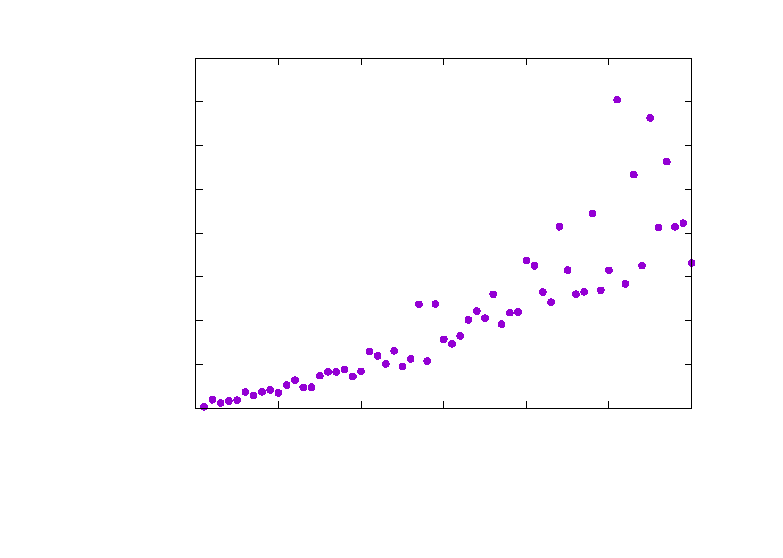
\includegraphics{benchmarks/lattice-bcs/embed-primes-exp}}%
    \gplfronttext
  \end{picture}%
\endgroup

%  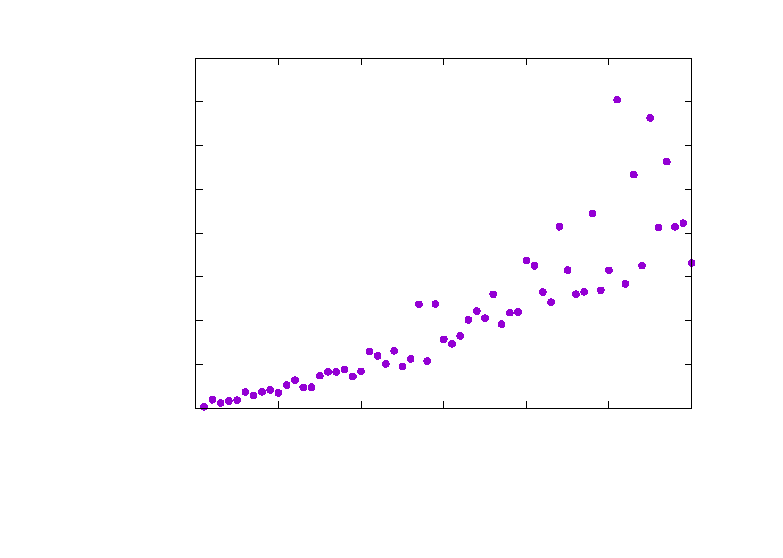
\includegraphics{benchmarks/lattice-bcs/embed-primes-exp.eps}
  \caption{Timings for the computation of embeddings from $\mathbb{F}_{p^{12}}$
  to $\mathbb{F}_{p^{24}}$ with $p$ a prime number growing up to approximately
  $2^{60}$.}
  \label{fig:bcs-embed-primes}
\end{figure}
Whether or not compatibility conditions have to be fufilled when computing an
embedding implies different internal routines in the Bosma-Canon-Steel
framework, such as intersections computations and recursive computations of
other embeddings. However, the different possible scenarios share the
preponderance of the root finding in the timings: it is the critical routine in
all cases. Although, for embeddings involving small degree finite fields and
with a low defect (\ie when other embeddings have already been computed and
information is known) the time spent dealing with high level routines can be
substantial. It is not really a problem because in that case the computations
are very fast, but it indicates that the Julia code could be optimized some
more.

% TODO
% ====
%
% Comparison with MAGMA?
%%


\chapter{Standard lattices of compatibly embedded finite field}
\label{chap:standard}
We have seen in Chapter~\ref{chap:lattice} two independant methods to create
lattices of compatibly embedded finite fields. In this chapter, we present a new
framework, inspired by both Conway polynomials and the Bosma-Canon-Steel
framework, that we call \emph{standard lattice of compatibly embedded finite
fields}.
\minitoc

% TODO: Figure

\clearpage

\paragraph{Outline of Chapter~\ref{chap:standard}.} In this chapter, we
construct new theoretic tools in order to build a new framework to manage finite
field extensions. Before studying these objects in details in the following
sections, we briefly explain our general strategy. If we have three integers
\[
  l\mid m\mid n,
\]
we can define embeddings between the finite fields
$\mathbb{F}_{p}(\zeta_l), \mathbb{F}_{p}(\zeta_m)$ and
$\mathbb{F}_{p}(\zeta_n)$, where $\zeta_l$ (resp. $\zeta_m, \zeta_n$) is a
primitive $l$-th (resp. $m$-th, $n$-th) root of unity.
\begin{center}
  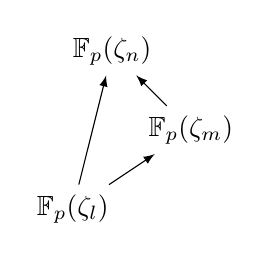
\begin{tikzpicture}
    \node (d) at (0, 0) {$\mathbb{F}_{p}(\zeta_l)$};
    \node (m) at (1.5, 1) {$\mathbb{F}_{p}(\zeta_m)$};
    \node (n) at (0.5, 2) {$\mathbb{F}_{p}(\zeta_n)$};

    \draw[arrow] (m) to (n);
    \draw[arrow] (d) to (m);
    \draw[arrow] (d) to (n);
  \end{tikzpicture}
\end{center}
Indeed, one can send $\zeta_l$ to $(\zeta_m)^{m/l}$ or to $(\zeta_n)^{n/l}$ to
embed $\mathbb{F}_p(\zeta_l)$ in either $\mathbb{F}_{p}(\zeta_m)$ or
$\mathbb{F}_p(\zeta_n)$. Similarly, one can send $\zeta_m$ to
$(\zeta_n)^{n/m}$ to obtain an embedding from $\mathbb{F}_{p}(\zeta_m)$ to
$\mathbb{F}_p(\zeta_n)$. In order to achieve compatibility between these
embeddings, one must have
\[
  ((\zeta_n)^{n/m})^{m/l} = (\zeta_m)^{m/l} = \zeta_l.
\]
This is essentially how Conway polynomials work: one
ensures that every finite field can be described as $\mathbb{F}_{p}(\zeta)$ for
some primitive root $\zeta$ that is compatible with every other primitive root.
A simple way of obtaining such a compatible configuration is to start from the root
$\zeta_n$ and compute $\zeta_l$ and $\zeta_m$ from $\zeta_n$.

We see in Section~\ref{sec:lenstra-allombert-embeddings} that this situation can
be generalized to arbitrary extensions $\mathbb{F}_{p^{l}}, \mathbb{F}_{p^{m}},
\mathbb{F}_{p^{n}}$ using the Lenstra-Allombert algorithm. Starting from a
primitive $n$-th root $\zeta_n$, one can compute the roots $\zeta_l, \zeta_m$
and construct the algebra $A_n =
\mathbb{F}_{p^{n}}\otimes\mathbb{F}_{p}(\zeta_n)$, and the corresponding
algebras $A_l$ and $A_m$. Then, from a solution $\alpha_n\in A_n$
of~\eqref{eq:h90-kummer} for $\zeta_n$, we can compute solutions $\alpha_l,
\alpha_m$ of~\eqref{eq:h90-kummer} in $A_l$ and $A_m$, and deduce compatible
embeddings between the finite fields $\mathbb{F}_{p^{l}},
\mathbb{F}_{p^{m}}, \mathbb{F}_{p^{n}}$.
\begin{center}
  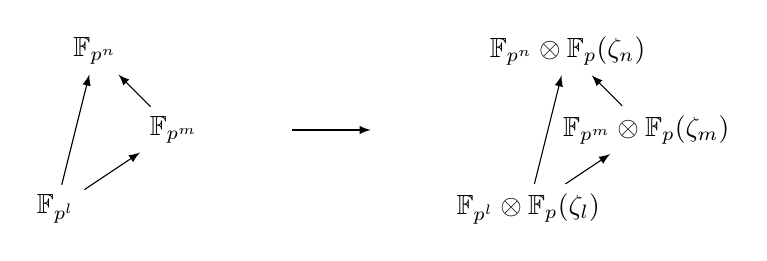
\begin{tikzpicture}
    \node (d) at (0, 0) {$\mathbb{F}_{p^l}$};
    \node (m) at (1.5, 1) {$\mathbb{F}_{p^m}$};
    \node (n) at (0.5, 2) {$\mathbb{F}_{p^n}$};

    \draw[arrow] (m) to (n);
    \draw[arrow] (d) to (m);
    \draw[arrow] (d) to (n);

    \draw[arrow] (3, 1) to (4, 1);

    \node (ad) at (6, 0) {$\mathbb{F}_{p^{l}}\otimes\mathbb{F}_{p}(\zeta_l)$};
    \node (am) at (7.5, 1) {$\mathbb{F}_{p^{m}}\otimes\mathbb{F}_{p}(\zeta_m)$};
    \node (an) at (6.5, 2) {$\mathbb{F}_{p^{n}}\otimes\mathbb{F}_{p}(\zeta_n)$};

    \draw[arrow] (am) to (an);
    \draw[arrow] (ad) to (am);
    \draw[arrow] (ad) to (an);

  \end{tikzpicture}
\end{center}
Because we can deduce compatible embeddings from a solution $\alpha$
of~\eqref{eq:h90-kummer} in a big algebra, we study the biggest algebra for a
given field of scalars $\mathbb{F}_{p^{a}}=\mathbb{F}_p(\zeta_{p^a-1})$, that we
call \emph{complete algebra}, and that is given by
\[
  A_{p^a-1} = \mathbb{F}_{p^{p^a-1}}\otimes \mathbb{F}_p(\zeta_{p^a-1}).
\]
These algebras are also the biggest algebras for a given level $a$.
We see in Section~\ref{sec:standardization} that the solutions $\alpha$
of~\eqref{eq:h90-kummer} for $\zeta_{p^a-1}$ in complete algebras all share a
very special property: they satisfy
\[
  \alpha^{p^a-1} = (\zeta_{p^a-1})^a,
\]
\ie they all have the same Kummer constant. We also see that the solutions
$\beta$ of~\eqref{eq:h90-kummer} in smaller Kummer algebras of the same level
$a$ that are computed from $\alpha$ also share the same Kummer constant.
Conversely, we can prove that the solutions that have the desired Kummer
constant 
\[
  c = (\zeta_{p^a-1})^a
\]
are linked with a solution $\alpha$ in the complete algebra of level $a$.
We thus call these special solutions \emph{standard}, and we show in
Section~\ref{sec:towards-standard-embeddings} how to construct compatible
embeddings from them, that we call \emph{standard embeddings}. Given a Kummer
algebra $A_n = \mathbb{F}_{p^{n}}\otimes \mathbb{F}_{p}(\zeta_n)$ of degree $a$,
we do not have to compute the complete algebra of degree $a$ in order to find a
standard solution in $A_n$, we can directly compute it in the smaller algebra
$A_n$. We call the pair $(A_n, \alpha_n)$, where $\alpha_n$ is a \emph{standard}
solution, a \emph{decorated algebra}. Decorated algebras allow us to compute
embeddings in an \emph{incremental} way, which is important when managing
finite field extensions. We finally show how to link complete algebras of
different levels in Section~\ref{sec:standard-embeddings}, so that two standard
solutions of~\eqref{eq:h90-kummer} in two arbitrary Kummer algebras can always
be used to compute a compatible embedding between the associated finite fields.
Again, in the general case of two arbitrary Kummer algebra, the computed
embedding is called \emph{standard}, and it is also compatible with future
embeddings, meaning that the framework is incremental. We then discuss the
implementation of the framework in
Section~\ref{sec:implementation-std-lattices}.

\section{The Lenstra-Allombert algorithm and lattices of embeddings}
\label{sec:lenstra-allombert-embeddings}

The two methods of Chapter~\ref{chap:lattice} both have their drawbacks: Conway
polynomials are expensive to compute and thus need to be precomputed, making
them inefficient for large extensions, while the Bosma-Canon-Steel framework
needs more computation each time an embedding is added to the lattice.
Our starting point in order to propose an alternative framework for lattices of
compatibly embedded finite fields is the Lenstra-Allombert algorithm and the
study of Kummer algebras done in Section~\ref{sec:kummer-algebras}. In all this
chapter, $\K=\mathbb{F}_p$ is a finite field of size $p$, where
$p$ is a prime number.

\subsection{From isomorphism to embedding}
\label{sec:iso-to-emb}

Let us first recall the Lenstra-Allombert \emph{isomorphism} algorithm. We keep
the notations of Section~\ref{sec:allombert}, where the details can be found.
Let $K$ and $L$ be two finite fields with $p^n$ elements, where $\gcd(p, n) =
1$, \ie
\[
  p\nmid n.
\]
We know that $K$ and $L$ are isomorphic and, if $\zeta$ is a primitive $n$-th
root of unity taken in the algebraic closure $\bar{\mathbb{F}}_p$ of $\K$, we know
% Note:
% =====
%
% We did not speak about algebraic closure in Chapter 5, where we introduce the
% notions of isomorphisms and algorithms to compute them. It is probably wise
% not to introduce that here only.
we can find an isomorphism by
finding two solutions $\alpha_K$ and $\alpha_L$ to the equation~\eqref{eq:h90-kummer}
\[
  (\sigma\otimes1)(\alpha) = (1\otimes\zeta)\alpha,
\]
respectively in $K\otimes\mathbb{F}_p(\zeta)$ and $L\otimes\mathbb{F}_p(\zeta)$.
We then compute $\kappa\in\mathbb{F}_p(\zeta)$ such that
\[
  1\otimes\kappa^n = \alpha_K^n/\alpha_L^n
\]
and the map
\[
  \phi:\first{\alpha_K}{\zeta}\mapsto\first{(1\otimes\kappa)\alpha_L}{\zeta}
\]
is then an isomorphism from $K$ to $L$. A key part of the algorithm is that the
root $\zeta$ must be the same in the two Kummer algebras
$K\otimes\mathbb{F}_p(\zeta)$ and $L\otimes\mathbb{F}_p(\zeta)$. In practice, it
means that we need to use elements that have the same minimal polynomial to
define $\zeta$ in both algebras. This constraint might seem easy to fulfill in
this case, but it becomes harder in the case of a \emph{compatible embedding}
computation. Assume that $m, n\in\mathbb{N}$ are two integers such that
\[
  m\mid n
\]
and $\gcd(p, m)=\gcd(p, n)=1$. Let $K$ be a finite field with $p^m$ elements and
$L$ a finite field with $p^n$ elements. We know that $K$ is isomorphic to a
subfield of $L$, \ie we have an embedding
\[
  K\emb L.
\]
To compute an embedding, one solution is to compute the algebras
$K\otimes\mathbb{F}_p(\zeta_m)$ and
$L\otimes\mathbb{F}_p(\zeta_m)$, where $\zeta_m$ is a primitive $m$-th root of
unity, as done in the isomorphism case, then compute solutions
$\alpha_{K, m}, \alpha_{L, m}$ of~\eqref{eq:h90-kummer} and the constant
$\kappa=\kappa_{K\emb L}$. This solution is satisfying as long as we only want
to compute a \emph{single} embedding in $L$. Indeed, assume we also have an
integer $l\in\mathbb{N}$ that divides $n$, such that $\gcd(p, l)=1$, and a
finite field $H$ of size $p^l$. Then there is an embedding
\[
  H\emb L,
\]
and in order to compute it we must find a primitive $l$-th root of unity
$\zeta_l$, compute $L\otimes\mathbb{F}_p(\zeta_l)$, compute a new solution
$\alpha_{L, l}$ of~\eqref{eq:h90-kummer} for $\zeta_l$ and the associated
constant $\kappa_{H\emb L}$. Therefore, each new embedding comes with the
computation of a new Kummer algebra, a new solution of~\eqref{eq:h90-kummer}, and a
new element $\kappa$. We must also store the elements $\kappa$ and the elements
defining the embeddings. Now, recall that if we want to use the Bosma-Canon-Steel
framework in order to compatibly embed $K$ in $L$, we must reccursively embed
the intersection $K\cap M$ in both fields $K$ and $M$, for each already
embedded subfield $M$ of $L$. 
\begin{center}
  \begin{tikzpicture}
    \node (K) at (0, 2) {$K$};
    \node (L) at (2, 4) {$L$};
    \node (M) at (4, 2) {$M$};
    \node (I) at (2, 0) {$K\cap M$};
    \node (?) at (1, 1) {\textbf{?}};
    \node (??) at (3, 1) {\textbf{?}};

    \draw[dashed-arrow] (K) to (L);
    \draw[arrow] (M) to (L);
    \draw[possible-arrow] (I) to (K);
    \draw[possible-arrow] (I) to (M);
  \end{tikzpicture}
\end{center}
This yields a quadratic memory complexity in the number of extensions in the
lattice and their degrees, as well as a quadratic number of new embedding
computations, \ie computations of Kummer algebras and solutions
of~\eqref{eq:h90-kummer}. It motivates a new solution with only one computation
of Kummer algebra and~\eqref{eq:h90-kummer} solution per extension in the lattice,
independently of the number of embedded subfields. Assume we have $\zeta_m$ and
$\zeta_n$ respectively two $m$-th and $n$-th primitive roots
of unity that are \emph{compatible}, \ie such that
\[
  (\zeta_n)^{n/m} = \zeta_m.
\]
We compute the Kummer algebras $K\otimes\mathbb{F}_{p}(\zeta_m)$ and
$L\otimes\mathbb{F}_p(\zeta_n)$, $\alpha_K$ a solution of~\eqref{eq:h90-kummer}
for the root $\zeta_m$ and $\alpha_L$ a solution of~\eqref{eq:h90-kummer} for
the root $\zeta_n$. In that case, the element
\[
  (\alpha_L)^{n/m}\in L\otimes\mathbb{F}_p(\zeta_n)
\]
is a solution of~\eqref{eq:h90-kummer} for the root $(\zeta_n)^{n/m}=\zeta_m$,
indeed
\begin{align*}
  (\sigma\otimes1)((\alpha_L)^{n/m}) &=
  ( (\sigma\otimes1)(\alpha_{L}))^{n/m} \\
  &= ( (1\otimes\zeta_n)\alpha_L)^{n/m}\\
  &= (1\otimes (\zeta_n)^{n/m})(\alpha_L)^{n/m}.
\end{align*}
The embedding $K\emb L$ is then described by
\[
  \first{\alpha_K}{\zeta_m}\mapsto\first{(1\otimes\kappa_{K\emb
  L})(\alpha_L)^{n/m}}{(\zeta_n)^{n/m}},
\]
where $\kappa_{K\emb L}\in\mathbb{F}_p(\zeta_n)$ is a $m$-th root of
$\alpha_L^n/\alpha_K^m$. There are still two issues with such a solution. First,
it is still necessary to store the constants $\kappa_{K\emb L}$ for each
embedding
\[
  K\emb L
\]
in the lattice. We would like these constants $\kappa$ to be equal to $1$, or
maybe that a close formula exists for these constants, by choosing special
solutions $\alpha$ of~\eqref{eq:h90-kummer}. We achieve the latter
by constructing \emph{standard} solutions of~\eqref{eq:h90-kummer} in
Section~\ref{sec:standard-solution}.

\subsection{Cyclotomic lattices}

The second, and most important, issue is the compatibility condition between the
roots of unity $\zeta$. When we write a compatibility condition like
\[
  \zeta_m = (\zeta_n)^{n/m},
\]
we implicitly state that there is a natural inclusion 
\[
  \mathbb{F}_p(\zeta_m)\subseteq\mathbb{F}_p(\zeta_n)
\]
that makes the embedding from $\mathbb{F}_{p}(\zeta_m)$ to
$\mathbb{F}_{p}(\zeta_n)$ trivial, \ie the embedding is the identity in that
case. In practice, this is not always the situation at hand. For example,
if for some reason the root $\zeta_m$ already exists in some field
$\mathbb{F}_{p^a}$ in the current state of our computer algebra system, and if the
root $\zeta_n$ lives in a strictly bigger field
$\mathbb{F}_{p^b}=\mathbb{F}_p(\zeta_n)$ that we have to compute, then the field
$\mathbb{F}_{p^a}$ is not included in the field $\mathbb{F}_{p^b}$, and the
embedding
\[
  \mathbb{F}_{p^a}\emb \mathbb{F}_{p^b}
\]
is not trivial. In the general case, if we want to use the Lenstra-Allombert
embedding algorithm, what we need is a \emph{cyclotomic
lattice}, given by Definition~\ref{defi:cyclotomic-lattice}.
\begin{defi}[Cyclotomic lattice]
  \label{defi:cyclotomic-lattice}
  A \emph{cyclotomic lattice} is composed of two things:
  \begin{itemize}
    \item a collection
  \[
    \mathcal S^I = \left\{ (K_m, \zeta_m) \right\}_{m\in I}
  \]
  over some support set $I\subset \mathbb{N}\setminus p\mathbb{N}$. The element
  $K_m$ is an explicitly represented finite extension of $\K=\mathbb{F}_p$, and
  the element $\zeta_m\in K_m$ is a generating element of $K_m$ that is also a
  primitive $m$-th root of unity, \ie we have
  \[
  K_m = \mathbb{F}_{p}(\zeta_m)
  \]
  and
  \[
  (\zeta_m)^m=1.
  \]
    \item explicit embeddings
      \[
        \begin{array}{llll}
          \iota_{m, n}: & K_m & \emb & K_n\\
          & \zeta_m & \mapsto & (\zeta_n)^{n/m}
        \end{array}
      \]
      whenever $(m, n)\in I^2$ are such that $m\mid n$.
  \end{itemize}
\end{defi}

Again, there is no problem if we know beforehand all the degrees of the
extensions in the lattice that we will use, \ie if the support set $I$ is
finite. Indeed, in that case there is an efficient randomised algorithm to
compute the cyclotomic lattice: consider
\[
  N = \lcm_{m\in I}(m)
\]
and construct the smallest finite field $\mathbb{F}_{p^a}$ such that $N$ divides
$p^a-1$, \ie the smallest finite field containing an $N$-th primitive root of
unity. Then take $x\in\mathbb{F}_{p^a}$ at random, compute 
\[
  y=x^{(p^a-1)/N}
\]
and check that the multiplicative order of $y$ is $N$. If it is, we can
construct all roots $\zeta_m$ as powers of this element:
\[
  \zeta_m = y^{N/m}
\]
for all $m\in I$, and we can set
\[
  K_m = \mathbb{F}_p(\zeta_m)\subset \mathbb{F}_{p^a}
\]
and let the embeddings $\iota_{m, n}$ be natural inclusions. But once again,
this methode does not produce an incremental lattice, thus it is not really user
friendly: one would like to have a lattice where new elements can be added on
the fly. Conway polynomials, that were introduced in
Section~\ref{sec:conway} in order to construct a lattice of
compatibly embedded finite fields, offer an other example of cyclotomic lattice. In
fact, a cyclotomic lattice is always a lattice of compatibly embedded finite
fields, because each time we have $l, m, n\in I$ with
\[
  l\mid n\mid n,
\]
we have
\[
  (\zeta_n)^{n/l} = ((\zeta_n)^{m/l})^{n/m}
\]
and it follows that
\[
  \iota_{l, n} = \iota_{m, n}\circ\iota_{l, m}.
\]
One can thus wonder why we need a structure than can be used to represent a
lattice of compatibly embedded finite fields, precisely to construct a lattice
of compatibly embedded finite fields. In fact, we will see in the next sections
that with a fairly small cyclotomic lattice, we are able to construct a much larger
lattice of compatibly embedded finite fields, thus making the whole construction
interesting, above all if the cyclotomic lattice is incremental, like with
Conway polynomials. In the next sections, we consider that we have an abstract
cyclotomic lattice, without specifying any particular construction. We only
assume that we have a collection $\mathcal S^I$ satisfying the conditions of
Definition~\ref{defi:cyclotomic-lattice}.

\subsection{Kummer embeddings}
\label{sec:kummer-embeddings}

As we have seen in the last sections, asking for a compatibility condition
\[
  \zeta_m = (\zeta_n)^{n/m}
\]
each time we want to use the Lenstra-Allombert embedding algorithm to embed
$\mathbb{F}_{p^m}$ in $\mathbb{F}_{p^n}$, in a compatible way, is not trivial:
it requires the availability of a cyclotomic lattice. Moreover, this equation
implies that there is a natural inclusion
\[
  \mathbb{F}_{p}(\zeta_m)\subset\mathbb{F}_{p}(\zeta_n),
\]
which is not the case in general. In order to be as thorough as possible, we
will thus write the image of $\zeta_m$ in the larger field
$\mathbb{F}_p(\zeta_n)$ as $\iota_{m, n}(\zeta_m)$. By definition, we have
\[
  \iota_{m, n}(\zeta_m) = (\zeta_{n})^{n/m}.
\]
We then generalize the discussion of Section~\ref{sec:iso-to-emb} and the
results of Section~\ref{sec:lenstra-allombert-isomorphism} in this setting. We
keep the ``Kummer algebra'' terminology, already used in
Section~\ref{sec:kummer-algebras}, that is based on~\cite{DRR19}. We now assume
that a cyclotomic lattice $\mathcal S^I$ is available. Let
\[
  m\mid n
\]
be two integers prime to $p$, we then have an embedding
\[
\begin{array}{cccc}
  \iota_{m, n}: & \mathbb{F}_{p}(\zeta_m)& \emb &\mathbb{F}_{p}(\zeta_n)\\
  & \zeta_m & \mapsto & (\zeta_n)^{n/m}.
\end{array}
\]
We also let
\[
  A_m=\mathbb{F}_{p^m}\otimes\mathbb{F}_{p}(\zeta_m)
\]
and
\[
  A_n=\mathbb{F}_{p^n}\otimes\mathbb{F}_{p}(\zeta_n)
\]
be two Kummer algebras. As was the case for
the Lenstra-Allombert \emph{isomorphism} algorithm, we want to deduce a field
embedding from an algebra embedding between $A_m$ and $A_n$, using the
properties of the solutions of~\eqref{eq:h90-kummer}. We are thus
interested in a special class of morphisms that are closely linked with
these solutions.
\begin{defi}[Kummer embedding]
  \label{defi:kummer-embedding}
  A \emph{Kummer embedding} of $A_m$ into $A_n$ is an injective
  $\K$-algebra morphism
  \[
    \Phi:A_m\emb A_n
  \]
  such that:
  \begin{itemize}
    \item the morphism $\Phi$ extends the scalar embedding
      $1\otimes\iota_{m,n}$;
    \item the morphism $\Phi$ commutes with $\sigma\otimes1$.
  \end{itemize}
\end{defi}
We can in fact give a simpler characterization of Kummer embeddings, and see that
they are of the form $\Phi=\phi\otimes\iota$, where $\iota$ is the embedding
described by the cyclotomic lattice $\mathcal S^I$. The embedding $\phi$ is then the one for
which we will try to obtain a description, using the properties of the solutions
of~\eqref{eq:h90-kummer}.
\begin{prop}
  \label{prop:correspondence-embeddings}
  There is a $1$-to-$1$ correspondence between Kummer embeddings
  \[
    \Phi:A_m\emb A_n
  \]
  and embeddings of finite fields
  \[
    \phi:\mathbb{F}_{p^m}\emb\mathbb{F}_{p^n},
  \]
  given by
  \[
    \Phi=\phi\otimes\iota_{m, n}\longleftrightarrow \phi.
  \]
  Moreover, this correspondence commutes with composition of embeddings.
\end{prop}
\begin{proof}
  We will prove that the correspondence is given by:
  \begin{itemize}
    \item if $\Phi$ is a Kummer embedding, then $\Phi$ maps
      $\mathbb{F}_{p^m}\otimes1$ into $\mathbb{F}_{p^n}\otimes1$. Thus the
      restriction of $\Phi$ to $\mathbb{F}_{p^m}$ is of the form $\phi\otimes1$
      for some embedding $\phi:\mathbb{F}_{p^m}\emb\mathbb{F}_{p^n}$, and we
      have $\Phi=\phi\otimes\iota_{m, n}$;
    \item conversely, if $\phi:\mathbb{F}_{p^m}\emb\mathbb{F}_{p^n}$ is an
      embedding of finite fields, then $\Phi=\phi\otimes\iota_{m, n}$ is a
      Kummer embedding.
  \end{itemize}
 Let $\Phi:A_m\emb A_n$ be a Kummer embedding. Since $\Phi$ is an algebra
 morphism, we have 
 \[
   \Phi(\beta^p) = \Phi(\beta)^p
 \]
for all $\beta\in A_m$. Since $(\sigma\otimes\sigma)(\beta) = \beta^p$, this
proves that $\Phi$ commutes with $\sigma\otimes\sigma$. It also
commutes with $\sigma\otimes1$, and thus with its inverse $\sigma^{-1}\otimes1$.
It then also commutes with
\[
  (\sigma^{-1}\otimes1)\circ(\sigma\otimes\sigma) = 1\otimes\sigma.
\]
Now, if $\beta\in\mathbb{F}_{p^m}\otimes1$, we know thanks
to Remark~\ref{rem:fixed-elems} that it is fixed by $1\otimes\sigma$, thus we have that
\begin{align*}
 (1\otimes\sigma)\circ\Phi(\beta) &= \Phi\circ(1\otimes\sigma)(\beta)\\
 &= \Phi(\beta).
\end{align*}
Again, using Remark~\ref{rem:fixed-elems}, we then know that
$\Phi(\beta)\in\mathbb{F}_{p^n}\otimes1$. This proves that
$\mathbb{F}_{p^m}\otimes1$ is mapped into $\mathbb{F}_{p^n}\otimes1$. Now, this
means that every element of the form $x\otimes1$ with $x\in\mathbb{F}_{p^m}$ is
mapped to an element of the form $\Phi(x\otimes1)=y\otimes1$ with $y\in\mathbb{F}_{p^m}$.
Because $\Phi$ is a morphism of algebras, if we
let $\phi(x)=y$, we can check that
\[
  \phi:\mathbb{F}_{p^m}\to\mathbb{F}_{p^n}
\]
is also a morphism. Therefore, the restriction of $\Phi$ on
$\mathbb{F}_{p^m}$ is of the form $\phi\otimes1$, where
$\phi:\mathbb{F}_{p^m}\emb\mathbb{F}_{p^n}$ is an embedding
of finite fields. We conclude that $\Phi=\phi\otimes\iota_{m, n}$. Indeed, if 
\[
  \beta=\sum_{j}x_j\otimes y_j
\]
is an element of the Kummer algebra $A_m$, we then have
\begin{align*}
  \Phi(\beta) &= \Phi(\sum_{j}x_j\otimes y_j) \\
  &= \sum_j\Phi(x_j\otimes y_j)\\
  &= \sum_j\Phi(x_j\otimes1)\times\Phi(1\otimes y_j)\\
  &= \sum_j(\phi\otimes1)(x_j\otimes1)\times(1\otimes\iota_{m, n})(1\otimes y_j)\\
  &= \sum_j (\phi(x_j)\otimes1)\times(1\otimes\iota_{m, n}(y_j))\\
  &= \sum_j \phi(x_j)\otimes\iota_{m, n}(y_j)\\
  &= \sum_j (\phi\otimes\iota_{m, n})(x_j\otimes y_j)\\
  &= (\phi\otimes\iota_{m, n})(\sum_jx_j\otimes y_j),
\end{align*}
and thus
\[
  \Phi(\beta) = (\phi\otimes\iota_{m, n})(\beta)
\]
for every element $\beta\in A_m$.

Conversely, if $\phi:\mathbb{F}_{p^{m}}\emb\mathbb{F}_{p^n}$ is an embedding of
finite fields and if we define
\[
  \Phi = \phi\otimes\iota_{m, n},
\]
we see that $\Phi$ is a morphism of $\K$-algebras that extends the scalar embedding
$\iota_{m, n}$ by definition.
The embedding $\phi$ is a power of the Frobenius automorphism $\sigma$ and thus
commutes with $\sigma$, hence $\sigma\otimes1$ commutes with
$\Phi=\phi\otimes\iota_{m, n}$, and this proves that $\Phi$ is a Kummer
embedding.

Now, if we have three Kummer algebras $A_l, A_m, A_n$ such that 
\[
  l\mid m\mid n
\]
and two Kummer embeddings $\Phi_{l, m}:A_l\emb A_m$ and $\Phi_{m, n}:A_m\emb
A_n$, we know that there exists $\phi_{l,
m}:\mathbb{F}_{p^l}\emb\mathbb{F}_{p^m}$ and $\phi_{m,
n}:\mathbb{F}_{p^{m}}\emb\mathbb{F}_{p^{n}}$ such that we have the following
diagram.
\begin{center}
    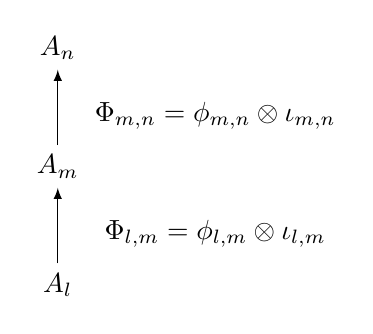
\begin{tikzpicture}
      \node (l) at (0, 0) {$A_l$};
      \node (m) at (0, 1.5) {$A_m$};
      \node (n) at (0, 3) {$A_n$};

      \draw[arrow] (l) -- (m);
      \draw[arrow] (m) -- (n);

      \node (f12) at (2, 0.65)
      {$\Phi_{l,m}=\phi_{l, m}\otimes\iota_{l, m}$};
      \node (f13) at (2, 2.15)
      {$\Phi_{m,n}=\phi_{m, n}\otimes\iota_{m, n}$};
    \end{tikzpicture}
\end{center}
Now the map $\Phi_{m, m}\circ\Phi_{l,m}$ is a Kummer embedding from $A_l$ into
$A_n$, hence there exist an embedding
$\phi:\mathbb{F}_{p^{l}}\emb\mathbb{F}_{p^{n}}$ such that 
\[
  \Phi_{m, m}\circ\Phi_{l,m}=\phi\otimes\iota_{l, n}.
\]
But we also have 
\[
  \Phi_{m, m}\circ\Phi_{l,m}=(\phi_{m, n}\circ\phi_{l,
  m})\otimes(\iota_{m, n}\circ\iota_{l, m}),
\]
and since $\iota_{l,n}=\iota_{m, n}\circ\iota_{l, m}$ by definition, we obtain
\[
  \phi_{m, n}\circ\phi_{l, m}=\phi,
\]
thus the correspondence commutes with compositions of embeddings.
\end{proof}
\begin{prop}
  \label{prop:correspondence-solutions}
  Let $\alpha_m\in A_m$ be a nonzero solution of~\eqref{eq:h90-kummer} for
  $\zeta_m$, and let $c_m$ be its Kummer constant. Then, there is a $1$-to-$1$
  correspondence between Kummer embeddings
  \[
    \Phi:A_l\emb A_m
  \]
  and solutions $\hat\alpha\in A_n$ of~\eqref{eq:h90-kummer} for
  $(\zeta_n)^{n/m}=\iota_{m, n}(\zeta_m)$ that also satisfy
  \[
    \hat\alpha^m = 1\otimes\iota_{m, n}(c_m).
  \]
  The correspondence is given by
  \[
    \Phi(\alpha_m) = \hat\alpha.
  \]
\end{prop}
\begin{proof}
Let $\Phi:A_m\emb A_n$ be a Kummer embedding. Lemma~\ref{lm:h90-solutions} shows
that $\alpha_m$ is a generator of $A_m$ as an $1\otimes\mathbb{F}_{p}(\zeta_m)$
algebra. Thus every element $\beta\in A_m$ can be written in the form
\[
  \beta = \sum_{j=0}^{m-1}(1\otimes b_j)(\alpha_m)^j,
\]
and we obtain
\[
  \Phi(\beta) = \sum_{j=0}^{m-1}(1\otimes\iota_{m, n}(b_j))\Phi(\alpha_m)^j,
\]
therefore we see that $\Phi$ is determined by its image $\Phi(\alpha_m)$. Moreover,
$\hat\alpha=\Phi(\alpha_m)$ is a solution of~\eqref{eq:h90-kummer} for
$(\zeta_n)^{n/m}=\iota_{m,n}(\zeta_m)$ that satisfies
$\hat\alpha^m=\iota_{m, n}(c_m)$. Indeed, this is a generalization of the
computations done in Section~\ref{sec:kummer-algebras} and a consequence of
Definition~\ref{defi:kummer-embedding}. We have
\begin{align*}
 (\sigma\otimes1)(\hat\alpha) &=(\sigma\otimes1)(\Phi(\alpha_m))\\
 &= \Phi( (\sigma\otimes1)(\alpha_m))\\
 &= \Phi((1\otimes\zeta_m)\alpha_m)\\
 &= (1\otimes\iota_{m, n})(\zeta_m)\Phi(\alpha_m)\\
 &= (1\otimes\iota_{m, n}(\zeta_m))\hat\alpha
\end{align*}
and
\begin{align*}
 \hat\alpha^m &= \Phi(\alpha_m)^m\\
 &= \Phi(\alpha_m^m)\\
 &= \Phi(1\otimes c_m)\\
 &= 1\otimes\iota_{m, n}(c_m).
\end{align*}

 Converserly, if $\hat\alpha$ is a solution of~\eqref{eq:h90-kummer} for
 $\iota_{m, n}(\zeta_m)$ such that $\hat\alpha^m=\iota_{m, n}(c_m)$, we see that
 \[
  \Phi(\beta) = \sum_{j=0}^{m-1}(1\otimes\iota_{m, n}(b_j))\hat\alpha^j,
 \]
 for any element
 \[
  \beta = \sum_{j=0}^{m-1}(1\otimes b_j)(\alpha_m)^j
 \]
 gives a well-defined morphism of algebras from  $A_m$ into $A_n$ that satisfies
 $\Phi(\alpha)=\hat\alpha$ and
 the conditions in Definition~\ref{defi:kummer-embedding}, \ie it extends
 $\iota_{m, n}$ and commutes with $\sigma\otimes1$.
\end{proof}
With these two correspondences, we can now describe a little more the link
between solutions of~\eqref{eq:h90-kummer} and the finite field embeddings
$\phi$ that we compute from them.
\begin{cor}
  \label{cor:link-h90-embedding}
  Let $\alpha_m\in A_m$ be a nonzero solution of~\eqref{eq:h90-kummer} for
  $\zeta_m$ with Kummer constant $c_m$ and let $\hat\alpha\in A_n$ be a solution
  of~\eqref{eq:h90-kummer} for $(\zeta_n)^{n/m}$ that satisfies
  $\hat{\alpha}^m=\iota_{m, n}(c_m)$. Then
  \begin{itemize}
    \item the solution $\hat{\alpha}$ belongs to the subset
      $\mathbb{F}_{p^{l}}\otimes\mathbb{F}_p((\zeta_n)^{n/m})\subset A_n$;
    \item the assignation
      $\first{\alpha_m}{\zeta_m}\mapsto\first{\hat\alpha}{(\zeta_n)^{n/m}}$
      defines an embedding $\phi:\mathbb{F}_{p^{m}}\emb\mathbb{F}_{p^{n}}$;
    \item the map $\Phi=\phi\otimes\iota_{m, n}$ is the unique Kummer embedding
      such that $\Phi(\alpha_m)=\hat\alpha$.
  \end{itemize}
\end{cor}
\begin{proof}
  By Proposition~\ref{prop:correspondence-solutions}, we know that there exists
  a unique Kummer embedding 
  \[
    \Phi:A_m\emb A_n
  \]
  such that $\Phi(\alpha_m) =
  \hat\alpha$. We also know thanks to
  Proposition~\ref{prop:correspondence-embeddings} that
  \[
    \Phi=\phi\otimes\iota_{m, n}
  \]
  for some embedding of finite fields
  $\phi:\mathbb{F}_{p^{m}}\emb\mathbb{F}_{p^{n}}$. If $\alpha_m =
  \sum_{j=0}^{a-1}x_j\otimes(\zeta_m)^j$, where $a$ is the level of $A_m$, we
  obtain
  \[
    \hat\alpha = \sum_{j=0}^{a-1}\phi(x_j)\otimes(\zeta_n)^{\frac{in}{m}},
  \]
  thus we have $\hat\alpha\in\mathbb{F}_{p^{m}}\otimes\mathbb{F}_{p}(
  (\zeta_n)^{n/m})$. We also see that $x_0=\first{\alpha_m}{\zeta_m}$ is mapped
  to $\phi(x_0) = \first{\hat\alpha}{(\zeta_n)^{n/m}}$, but
  $\first{\alpha_m}{\zeta_m}$ is a generating element of
  $\mathbb{F}_{p^{m}}$ by Proposition~\ref{prop:generate}, hence the assignation
  \[
    \first{\alpha_m}{\zeta_m}\mapsto\first{\hat\alpha}{(\zeta_n)^{n/m}}
  \]
  defines $\phi$.
\end{proof}
With these results we are ready to generalize
Proposition~\ref{prop:lenstra-allombert-algorithm} to the embedding case, with
the cyclotomic lattice setting, giving a minor variation of the original
algorithm of Allombert.
\begin{algorithm}
  \caption{(Allombert's algorithm)}
  \label{algo:allombert}
  \begin{algorithmic}[1]
    \Require{$\mathbb{F}_{p^m}, \mathbb{F}_{p^n}$, for $m\mid n$ integers prime to $p$,
    and a cyclotomic lattice $\mathcal S^{\{l,m\}}$.}
    \Ensure{$s\in \mathbb{F}_{p^m}, t\in\mathbb{F}_{p^n}$, such that the assignation $s\mapsto t$
    defines an embedding $\phi:\mathbb{F}_{p^{m}}\emb\mathbb{F}_{p^n}$.}
  \State Construct the Kummer algebras $A_m$ and $A_n$.
  \State Find $\alpha_m\in A_m$ and $\alpha_n\in A_n$, nonzero solutions
  of~\eqref{eq:h90-kummer} for $\zeta_m$
  and $\zeta_n$ respectively.
  \State Compute their Kummer constants: $(\alpha_m)^m=1\otimes c_m$ and
  $(\alpha_n)^n=1\otimes c_n$.
  \State Compute $\kappa$, a $m$-th root of $\iota_{m, n}(c_m)/c_n$.
  \State Return $\first{\alpha_{m}}{\zeta_m}$ and
  $\first{(1\otimes\kappa)(\alpha_n)^{\frac{n}{m}}}{(\zeta_n)^{\frac{n}{m}}}$.
  \end{algorithmic}
\end{algorithm}
\begin{prop}
  \label{prop:allombert-works}
  Algorithm~\ref{algo:allombert} is correct: it returns elements that define an
  embedding $\phi:\mathbb{F}_{p^{m}}\emb\mathbb{F}_{p^{n}}$.
\end{prop}
\begin{proof}
  The ideas of the proof are the same as the ones found in the proof of
  Proposition~\ref{prop:lenstra-allombert-algorithm}, which were already present
  in the simpler case of Proposition~\ref{prop:allombert-simple}, where all the
  roots of unity are in $\K$. By
  Proposition~\ref{prop:correspondence-embeddings}, let 
  \[
    \Phi=\phi\otimes\iota_{m, n}
  \]
  be a Kummer embedding from $A_m$ into $A_n$. Let $\alpha_m\in A_m$ a solution
  of~\eqref{eq:h90-kummer} for $\zeta_m$ with Kummer constant $c_m$, and let
  $\alpha_n\in A_n$ a solution of~\eqref{eq:h90-kummer} for $\zeta_n$ with
  Kummer constant $c_n$. By
  Proposition~\ref{prop:correspondence-solutions}, there is a solution $\hat\alpha\in
  A_n$ of~\eqref{eq:h90-kummer} for $(\zeta_n)^{n/m}$ that satisfies
  $\hat{\alpha}^m=\iota_{m, n}(c_m)$ and such that $\Phi(\alpha_m)=\hat\alpha$.
  Now, we also have that $(\alpha_n)^{n/m}$ is a solution
  of~\eqref{eq:h90-kummer} for $(\zeta_n)^{n/m}$, and the solutions
  of~\eqref{eq:h90-kummer} for $(\zeta_n)^{n/m}$ form a one-dimensional
  $1\otimes\mathbb{F}_{p}(\zeta_n)$-vector space, so there exists a constant
  $\lambda\in\mathbb{F}_{p}(\zeta_n)$ such that
  \[
    \hat\alpha = (1\otimes\lambda)(\alpha_n)^{n/m}.
  \]
  We conclude that 
  \[
    \cfrac{\iota_{m, n}(c_m)}{c_n} = \lambda^m
  \]
  is a $m$-th root in $\mathbb{F}_{p}(\zeta_n)$. If we let
  \[
    \kappa = (\zeta_n)^{\frac{in}{m}}\lambda,
  \]
  for some integer $i$, be a $m$-th root of $\frac{\iota_{m, n}(c_m)}{c_n}$, it
  follows that
  \[
    \tilde\alpha = (1\otimes\kappa)(\alpha_n)^{n/m} =
    (1\otimes(\zeta_n)^{\frac{in}{m}})\hat\alpha
  \]
  is a solution of~\eqref{eq:h90-kummer} for $(\zeta_n)^{n/m}$ that satisfies
  $\tilde\alpha^m = \iota_{m,n}(c_m)$. By
  Corollary~\ref{cor:link-h90-embedding}, we know that the assignation
  \[
    \first{\alpha_m}{\zeta_m}\mapsto\first{\tilde\alpha}{(\zeta_n)^{n/m}}
  \]
  defines an embedding from $\mathbb{F}_{p^m}$ into $\mathbb{F}_{p^{n}}$.
\end{proof}
\begin{rem}
  Taking the same notations as the one in the proof of
  Proposition~\ref{prop:allombert-works}, we see that the embedding returned by
  the algorithm is $\sigma^i\circ\phi$. Indeed, we have
  \begin{align*}
    \tilde\alpha &= (1\otimes(\zeta_n)^{\frac{in}{m}})\hat\alpha\\
    &= (\sigma\otimes1)^i(\hat\alpha)\\
    &= (\sigma^i\otimes1)(\hat\alpha).
  \end{align*}
  If we let $x_0=\first{\hat\alpha}{(\zeta_n)^{\frac{n}{m}}}$, we wee that the
  returned embedding is defined by the assignation
  \[
    \first{\alpha_m}{\zeta_m}\mapsto\sigma^i(x_0)
  \]
  while $\phi$ is defined by
  \[
    \first{\alpha_m}{\zeta_m}\mapsto x_0.
  \]
\end{rem}
\section{Standard solution of Hilbert $90$}
\label{sec:standard-solution}

\subsection{Complete algebras and standardization}
\label{sec:standardization}

We discussed in Section~\ref{sec:iso-to-emb} the 
obstacles when constructing a lattice of compatibly embedded finite fields using
the Lenstra-Allombert algorithm. The first one is that we need to have compatibility
between the roots of unity that we use, and that can be hard to obtain in
practice. We solved that problem by assuming the availability of a
cyclotomic lattice $\mathcal S^I$, and we proved that all the results concerning
the Lenstra-Allombert algorithm can be expressed in that setting in
Section~\ref{sec:kummer-embeddings}. Now, we can obtain compatibility by
replacing the naive embedding algorithm by the Lenstra-Allombert algorithm in
the Bosma-Canon-Steel framework. This solutions immediately gives a compatible
lattice of embedded finite fields. Still, among the sub-goals presented in
Section~\ref{sec:compatibility-problem} that such a lattice may achieve, there
are two of them on which we would like to improve.
\begin{description}
  \item[\emph{Uniqueness:}] the element $\first{\lambda_m}{\zeta_m}$ is
    a generator of $\mathbb{F}_{p^{m}}$, or equivalently, it provides an
    irreducible polynomial in $\K[X]$ of degree $m$. However this polynomials
    depends on the choice of $\alpha_l$, because it depends on the Kummer constant
    $c_l$ of $\alpha_l$ by Proposition~\ref{prop:kummer-constant}, thus there is
    no uniqueness.
  \item[\emph{Compatibility:}] the embedding of finite fields
    $\phi:\mathbb{F}_{p^{m}}\to\mathbb{F}_{p^{n}}$ depends on
    the choice of the constant $\kappa$, which itself depends on the choice of
    the solutions $\alpha_m$ and $\alpha_n$ of \eqref{eq:h90-kummer}, and also
    of the choice of a $m$-th root of unity. In order to achieve compatibility,
    we must keep track of the constants $\kappa$ for each embedding computation
    \[
      \mathbb{F}_{p^{m}}\emb\mathbb{F}_{p^{n}}
    \]
    in the
    lattice, which grow quadratically with the number of fields, because of the
    common subfield compatibility condition in the Bosma-Canon-Steel framework.
\end{description}
In this section and in Section~\ref{sec:standard-embeddings}, we will see how to
choose special solutions of \eqref{eq:h90-kummer}, in order to manage these
constants $\kappa$. Our dream would be to be able to choose the solutions
of~\eqref{eq:h90-kummer} in a way that makes the constants trivial, \ie 
\[
  \kappa_{\mathbb{F}_{p^{m}}\emb \mathbb{F}_{p^{n}}} = 1.
\]
From Algorithm~\ref{algo:allombert}, we see that the constant
$\kappa_{\mathbb{F}_{p^{m}}\emb\mathbb{F}_{p^{n}}}$ is a $m$-th root of the
quotient
\[
  \cfrac{\iota_{m, n}(c_m)}{c_n},
\]
thus the condition $\kappa_{\mathbb{F}_{p^{m}}\emb\mathbb{F}_{p^{n}}}=1$ implies
\[
  \iota_{m, n}(c_m) = c_n,
\]
which in turn implies that $c_n$ belongs to the subset
\[
  \mathbb{F}_{p}( (\zeta_n)^{\frac{n}{m}})\subseteq\mathbb{F}_p(\zeta_n).
\]
This could possibly fail if the Kummer algebras $A_m$ and $A_n$ are of distinct
level, \ie if their field of scalars are different. This motivates the study of
Kummer algebras of a given level, and the introduction of the notion of
\emph{complete} algebra.
\begin{defi}[Complete Kummer algebra]
  A Kummer algebra is \emph{complete} if it is of the largest degree for a given
  level.
\end{defi}
Therefore, the complete Kummer algebra of level $a$ is the Kummer algebra
\begin{align*}
  A_{p^a-1} &=
  \mathbb{F}_{p^{p^a-1}}\otimes\mathbb{F}_p(\zeta_{p^a-1})\\
  &=\mathbb{F}_{p^{p^a-1}}\otimes\mathbb{F}_{p^{a}}
\end{align*}
with field of scalars
\[
  \mathbb{F}_{p^{a}}\cong \mathbb{F}_p(\zeta_{p^a-1}).
\]
given by the element $\zeta_{p^a-1}$ in the cyclotomic lattice $\mathcal S^I$.
In fact these algebras have an interesting property.
\begin{lm}
  All nonzero solutions $\alpha_{p^a-1}\in A_{p^a-1}$ of~\eqref{eq:h90-kummer}
  for $\zeta_{p^a-1}$ have the same Kummer constant
  \[
    c_{p^a-1} = (\zeta_{p^a-1})^{a}.
  \]
\end{lm}
\begin{proof}
  \label{lm:complete-algebra-solutions}
  Let $\alpha_{p^a-1}\in A_{p^a-1}$ a solution of~\eqref{eq:h90-kummer} for
  $\zeta_{p^a-1}$. For all $\beta\in A_{p^a-1}$, we have $\beta^p = \sigma\otimes\sigma(\beta) =
  \beta^p$, so we also obtain 
  \[
    (\alpha_{p^a-1})^{p^a} = (\sigma^a\otimes\sigma^a)(\alpha_{p^a-1}).
  \]
  Now, we know that $\sigma^a$ is the identity on $\mathbb{F}_{p^a}$, hence we
  have
  \begin{align*}
    (\alpha_{p^a-1})^{p^a} &= (\sigma^a\otimes1)(\alpha_{p^a-1}) \\
    &= (1\otimes\zeta_{p^a-1})^a \alpha_{p^a-1}.
  \end{align*}
  Since $\alpha_{p^a-1}$ is invertible by Lemma~\ref{lm:h90-solutions}, we
  obtain that
  \[
    (\alpha_{p^a-1})^{p^a-1} = 1\otimes c_{p^a-1} = (1\otimes \zeta_{p^a-1})^a
  \]
  and it follows that
  \[
    c_{p^a-1} = (\zeta_{p^a-1})^{a}.
  \]
\end{proof}
Now this result is very important because we know that the degree $p^a-1$
irreducible polynomial in $\K[X]$ derived from the solution $\alpha_{p^a-1}$,
\ie the minimal polynomial of the element
$\first{\alpha_{p^a-1}}{\zeta_{p^a-1}}$,
only depends on the Kummer constant $c_{p^a-1}$ of $\alpha_{p^a-1}$, thus it
means that all solutions give the same polynomial. This will be the central idea
behind the notion of \emph{standard} elements.
\begin{defi}[Standard Kummer constant]
  Let $m$ be an integer prime to $p$. We define the \emph{standard Kummer
  constant} of order $m$ as
  \[
    \stdc{m} = (\iota_{m,
    p^a-1})^{-1}((\zeta_{p^a-1})^a)\in\mathbb{F}_{p}(\zeta_m),
  \]
  where $a=\nu(m)$ is the level of the Kummer algebra $A_m$.
\end{defi}
\begin{rem}
 Since $A_m$ is of level $a$, we have
 \[
   \mathbb{F}_p(\zeta_m) \cong \mathbb{F}_p(\zeta_{p^a-1}),
 \]
 hence the map $\iota_{m, p^a-1}$ is an isomorphism and $\stdc{m}$ is
 well-defined.
\end{rem}
\begin{defi}[Standard solution]
  Let $m$ be an integer prime to $p$. We say that a solution $\alpha_m\in A_m$
  is \emph{standard} if its Kummer constant is standard, \ie if we have
  \[
    (\alpha_m)^m = 1\otimes\stdc{m}.
  \]
\end{defi}
\begin{defi}[Decorated Kummer algebra]
  Let $m$ be an integer prime to $p$. We define a \emph{decorated Kummer
  algebra} as a pair
  \[
    (A_m, \alpha_m),
  \]
  where $\alpha_m$ is a standard solution of~\eqref{eq:h90-kummer} for
  $\zeta_m$.
\end{defi}
It follows from Lemma~\ref{lm:complete-algebra-solutions} that all nonzero
solutions of~\eqref{eq:h90-kummer} in a complete algebra are standard. This is
no longer the case in a non complete Kummer algebra, but we can still find
standard solutions.
\begin{prop}
  \label{prop:decoration}
 Let $m$ be an integer prime to $p$. Then $A_m$ can be decorated, \ie it admits a
 standard solution $\alpha_m$. Moreover, this solution $\alpha_m$ is unique up
 to a $m$-th root of unity. 
\end{prop}
\begin{proof}
 Let $a=\nu(m)$ be the level of $A_m$ and let $\alpha_m'\in A_m$ be a nonzero solution
 of~\eqref{eq:h90-kummer} for $\zeta_m$. Let also $\alpha_{p^a-1}$ be a nonzero
 solution of~\eqref{eq:h90-kummer} for $\zeta_{p^a-1}$, then it is standard by
 Lemma~\ref{lm:complete-algebra-solutions}. The element 
 \[
   (\alpha_{p^a-1})^{\frac{p^a-1}{m}}
 \]
 is a solution of~\eqref{eq:h90-kummer} for
 \[
   \iota_{m, p^a-1}(\zeta_m) = (\zeta_{p^a-1})^{\frac{p^a-1}{m}}.
 \]
 Now let
 \[
   \Phi:A_m\emb A_{p^a-1}
 \]
 be a Kummer embedding and let
 \[
   \hat\alpha = \Phi(\alpha_m'),
 \]
 then $\hat\alpha$ is also a solution of~\eqref{eq:h90-kummer} for
 $\iota_{m, p^a-1}(\zeta_m)$ and thus there exists a scalar
 $\lambda\in\mathbb{F}_p(\zeta_{p^a-1})$ such that
 \[
   (\alpha_{p^a-1})^{\frac{p^a-1}{m}} = (1\otimes\lambda)\hat{\alpha} .
 \]
 If we let
 \[
   \tilde\lambda = \iota_{m, p^a-1}^{-1}(\lambda),
 \]
 we obtain
 \begin{align*}
   (\alpha_{p^a-1})^{\frac{p^a-1}{m}} &= (1\otimes\lambda)\Phi(\alpha_m') \\
   &= \Phi( (1\otimes\tilde\lambda)\alpha_m').
 \end{align*}
If we set 
\[
  \alpha_m = (1\otimes\tilde\lambda)\alpha_m',
\]
it follows that
\begin{align*}
  \Phi((\alpha_m)^m) &= (\alpha_{p^a-1})^{p^a-1} \\
  &= 1\otimes(\zeta_{p^a-1})^a,
\end{align*}
therefore
\begin{align*}
  (\alpha_m)^m &= 1\otimes\iota_{m, p^a-1}^{-1}( (\zeta_{p^a-1})^a) \\
  &= 1 \otimes \stdc{m}
\end{align*}
and $\alpha_m$ is standard. If $\beta\in A_m$ is another solution
of~\eqref{eq:h90-kummer} for $\zeta_m$, then there exists a scalar
$\mu\in\mathbb{F}_p(\zeta_m)$ such that
\[
  \alpha_m= (1\otimes\mu)\beta,
\]
but then we obtain
\[
  (\alpha_m)^m = (1\otimes\mu^m)\beta^m.
\]
As a consequence, $\beta$ is standard if and only if $\mu^m = 1$ and the
standards solutions are the
\[
  (1\otimes\zeta_m^u)\alpha_m
\]
for $0\leq u\leq m-1$.
\end{proof}
From Proposition~\ref{prop:decoration}, it follows that for any integer $m$
prime to $p$, we can define $\mathbb{F}_{p^{m}}$ in a standard way.
\begin{defi}[Standard generating element]
  A generating element $x\in\mathbb{F}_{p^{m}}$ is called \emph{standard} if it
  is of the form
  \[
    x = \first{\alpha_m}{\zeta_m}
  \]
  for $\alpha_m\in A_m$ a standard solution of~\eqref{eq:h90-kummer}.
\end{defi}
\begin{defi}[Standard defining polynomial]
  The \emph{standard defining polynomial} $P_m$ for $\mathbb{F}_{p^{m}}$ is the
  minimal polynomial over $\K$ of a standard generating element of
  $\mathbb{F}_{p^{m}}$.
\end{defi}
\begin{defi}[Decorated finite field]
  Let $m\in\mathbb{N}$ an integer prime to $p$. A \emph{decorated finite field}
  is a pair $(\mathbb{F}_{p^{m}}, s_m)$ where $s_m\in\mathbb{F}_{p^{m}}$ is a
  standard generating element.
\end{defi}
\begin{rem}
  By Remark~\ref{rem:recover-alpha}, we can recover $\alpha_m$ the standard
  solution of~\eqref{eq:h90-kummer} from the standard generating element $s_m$,
  thus decorated Kummer algebras can be recovered from
  decorated finite fields.
\end{rem}
By Proposition~\ref{prop:kummer-constant}, we know that $P_m$ is entirely 
determined by $\stdc{m}$, and thus by the cyclotomic lattice $\mathcal S^I$ up
to order $p^a-1$, with $a=\nu(m)$ the level of $m$. This helps to achieve the
\emph{uniqueness} sub-goal of our lattice, because once the cyclotomic lattice
has been chosen, the standard defining polynomials are unique. As an example, we
give in Table~\ref{tab:std-polys} the first ten standard defining polynomials
induced by the cyclotomic lattice given by the Conway polynomials with $p=2$.
\begin{table}
  \centering
  \begin{tabular}{l}
    $x+1$ \\
    $x^3+x+1$ \\
    $x^5+x^3+1$ \\
    $x^7+x+1$ \\
    $x^9+x^7+x^4+x^2+1$\\
    $x^{11}+x^8+x^7+x^6+x^2+x+1$\\
    $x^{13}+x^{10}+x^5+x^3+1$\\
    $x^{15}+x+1$ \\
    $x^{17}+x^{11}+x^{10}+x^8+ x^7+x^6+x^4+x^3+x^2+x+1$ \\
    $x^{19}+x^{17}+x^{16}+x^{15}+x^{14}+x^{13}+x^{12}+x^8+x^7+x^6+x^5+x^3+1$
  \end{tabular}
  \caption{The first ten standard polynomials derived from Conway
    polynomials for $p=2$.}
  \label{tab:std-polys}
\end{table}
A small variation of the Lenstra-Allombert algorithm, given by
Algorithm~\ref{algo:decoration}, allows us to compute all these standard
elements.
\begin{algorithm}
  \caption{(Decoration -- Standardization)}
  \label{algo:decoration}
  \begin{algorithmic}[1]
    \Require {$\mathbb{F}_{p^m}$, for $m$ prime to $p$, and $\mathcal{S}^I$ a cyclotomic lattice.}
    \Ensure {$(A_m,\alpha_m)$ decorated, $P_m$ standard irreducible polynomial of degree $m$,
      and $s\in\mathbb{F}_{p^m}$ standard generating element inducing $\mathbb{F}_{p^m}\simeq\mathbb{F}_{p}[T]/(P_m)$.}
  \State Compute the Kummer algebra $A_m$.
  \State Compute $\stdc{m}=(\iota_{m, p^a-1})^{-1}((\zeta_{p^a-1})^a)\in\mathbb{F}_p(\zeta_m)$.
  \State Find $\alpha'_m\in A_m$ a nonzero solution of~\eqref{eq:h90-kummer} for $\zeta_m$.
  \State Compute its Kummer constant: $(\alpha'_m)^m=1\otimes c'_m$.
  \State Compute $\kappa$ a $m$-th root of $\stdc{m}/ c'_m$.
  \State Set $\alpha_{m}=(1\otimes\kappa)\alpha'_m$.
  \State Compute $P_m$ the minimal polynomial of $\first{\alpha_{m}}{\zeta_m}$
  over $\K$.
  \State Return $(A_m,\alpha_m)$, $P_m$, and $\first{\alpha_m}{\zeta_m}$.
  \end{algorithmic}
\end{algorithm}
\begin{prop}
  Algorithm~\ref{algo:decoration} is correct, \ie the computed element
  $\alpha_m$ is indeed standard. 
\end{prop}
\begin{proof}
  By Proposition~\ref{prop:decoration}, we know that there exists a standard
  solution of~\eqref{eq:h90-kummer} for $\zeta_m$, let $\pmb{\alpha}\in A_m$ be such a
  solution. Let $\alpha_m'\in A_m$ be any nonzero solution
  of~\eqref{eq:h90-kummer} for $\zeta_m$ and let $c_m'$ be its Kummer constant.
  Then we know that there exists $\lambda\in\mathbb{F}_p(\zeta_m)$ a scalar such that
  \[
    \pmb\alpha = (1\otimes\lambda)\alpha_m'.
  \]
  It follows that 
  \[
    \stdc{m} = \lambda^m c_m',
  \]
  thus 
  \[
    \stdc{m}/c_m'
  \]
  is indeed a $m$-th power. If we let $\kappa$ be a $m$-th root of
  $\stdc{m}/c_m'$ and if we set 
  \[
    \alpha_m = (1\otimes\kappa)\alpha_m',
  \]
  we obtain
  \[
    (\alpha_m)^m = 1\otimes\stdc{m}.
  \]
  We have thus proven that $\alpha_m$ is a standard solution
  of~\eqref{eq:h90-kummer} for $\zeta_m$. By definition,
  $\first{\alpha_m}{\zeta_m}$ is then a standard generating element of
  $\mathbb{F}_{p^{m}}$ and its minimal polynomial $P_m$ is a standard defining
  polynomial.
\end{proof}

\subsection{Towards standard embeddings}
\label{sec:towards-standard-embeddings}

Now that we have found a way to compute standard solutions
of~\eqref{eq:h90-kummer}, and to deduce standard generating elements to define
our finite fields, it is natural to work towards the definition of compatible
embeddings between these finite fields that are also standard. Our goal is also
to simplify the storage of the constants $\kappa$ involved in the computation of
such embeddings.
\begin{prop}
  \label{prop:power-compatibility}
  Let $m\mid n$ be two integers prime to $p$ and such that 
  \[
    \nu(m) = \nu(n),
  \]
  \ie the (decorated) Kummer algebras $(A_m, \alpha_m)$ and $(A_n, \alpha_n)$
  have the same level. Then there is a unique Kummer embedding
  \[
    \stdemb{m}{n}:A_m\emb A_n
  \]
  such that
  \[
    \stdemb{m}{n}(\alpha_m) = (\alpha_n)^{\frac{n}{m}}.
  \]
\end{prop}
\begin{proof}
  The element $\hat\alpha = (\alpha_n)^{\frac{n}{m}}$ is a solution
  of~\eqref{eq:h90-kummer} for $(\zeta_n)^{\frac{n}{m}}=\iota_{m, n}(\zeta_m)$.
  We also know that the Kummer constant of $\alpha_m$ is
  \[
    \stdc{m} = \iota_{m, p^a-1}^{-1}((\zeta_{p^a-1})^a)
  \]
  and the Kummer constant of $\alpha_n$ is 
  \[
    \stdc{n} = \iota_{n, p^a-1}^{-1}((\zeta_{p^a-1})^a).
  \]
  The embeddings $\iota$ are compatible by definition, thus we have
  \[
    \iota_{m, p^a-1} = \iota_{n, p^a-1}\circ\iota_{m, n}
  \]
  and
  \[
    \iota_{n, p^a-1}^{-1} = \iota_{m, n}\circ\iota_{m, p^a-1}^{-1}.
  \]
  It follows that
  \[
    \stdc{n} = \iota_{m, n}(\stdc{m}).
  \]
  By Proposition~\ref{prop:correspondence-solutions}, there exists a unique
  Kummer embedding $\stdemb{m}{n}$ such that
  \[
    \stdemb{m}{n}(\alpha_m) = \hat\alpha = (\alpha_n)^{\frac{n}{m}}.
  \]
\end{proof}
Proposition~\ref{prop:power-compatibility} guarantees that decorated Kummer
algebras $(A_m, \alpha_m), (A_n, \alpha_n)$ of the same level are
\emph{power-compatible}, \ie we can describe a unique Kummer embedding by
\[
  \alpha_m\mapsto (\alpha_n)^{\frac{n}{m}}.
\]
Therefore, there is no constant $\kappa$ to store in this case because we are in
the trivial case $\kappa=1$, which was our
goal. However, we see that power compatibility implies
\[
  \stdc{n} = \iota_{m, n}(\stdc{m}),
\]
hence implies that the decorated Kummer algebras share the same level. If the
Kummer algebras do not share the same level, we can ask for
\emph{norm-compatibility} instead of power-compatibility, at least between two
\emph{complete} decorated Kummer algebras. 
Let us first describe what ``norm'' we will be using.
Let $A_n$ be a Kummer algebra of level $\nu(n) = b$, so that
\[
  A_n = \mathbb{F}_{p^{n}}\otimes\mathbb{F}_{p^{b}}\cong
  \mathbb{F}_{p^{n}}\otimes\mathbb{F}_{p}(\zeta_{p^b-1}),
\]
where the isomorphism is given by $1\otimes\iota_{n, p^b-1}$. Then, if $a\mid b$
is another integer, the subalgebra of $A_n$ invariant under $1\otimes\sigma^a$
is identified (by the same isomorphism) with
\[
  (A_n)^{1\otimes\sigma^a} \cong \mathbb{F}_{p^{n}}\otimes\mathbb{F}_p(
  (\zeta_{p^b-1})^{\frac{p^b-1}{p^a-1}})
\]
where
\[
  (\zeta_{p^b-1})^{\frac{p^b-1}{p^a-1}} =
  N_{\mathbb{F}_{p^{n}}/\mathbb{F}_{p^{a}}}(\zeta_{p^b-1}) = \iota_{p^a-1,
  p^b-1}(\zeta_{p^a-1})
\]
and where $N_{\mathbb{F}_{p^{n}}/\mathbb{F}_{p^{a}}}$ is the relative norm of
the finite field extension
\[
  \mathbb{F}_{p^{b}}/\mathbb{F}_{p^{a}}.
\]
\begin{defi}[Scalar norm operator]
  Let $n$ an integer prime to $p$ and $A_n$ a Kummer algebra of level
  $\nu(n)=c$. Let $a,b$ two integers such that $a\mid b \mid c$,
  then we define the \emph{scalar norm operator} as
  \[
    \begin{array}{cccc}
      \mathcal N_{b/a,\, A_n}: & (A_n)^{1\otimes\sigma^b} & \to &
      (A_n)^{1\otimes\sigma^a}\\
      & \gamma & \mapsto & \prod_{0\leq j\leq
        \frac{a}{b}}(1\otimes\alpha^{ja})(\gamma)
    \end{array}
  \]
\end{defi}
This operator is well-defined, as the elements in the image of $\mathcal
N_{b/a,\, A_n}$ are indeed invariant under $1\otimes\sigma^a$. We often 
omit $A_n$ and only write $\N_{b/a}$, as the ambient space $A_n$ is
implicit. By construction, $\N_{b/a}$ acts on the scalar field
$1\otimes\mathbb{F}_{p^b}^\times$ as the usual norm $1\otimes
N_{\mathbb{F}_{p^{b}}/\mathbb{F}_{p^{a}}}$. Scalar norms are
\emph{multiplicative}, \ie for any $\gamma, \gamma'\in A_n$, we have
\[
  \N_{b/a}(\gamma\gamma') = \N_{b/a}(\gamma)\N_{b/a}(\gamma'),
\]
they are \emph{transitive}, \ie for any $a\mid b\mid c$, we have
\[
  \N_{c/a} = \N_{b/a}\circ\N_{c/b},
\]
and they commute with $\sigma\otimes1$. All these nice properties make the
scalar norm an excellent candidate to generalize the powering used to define
standard embeddings between decorated Kummer algebras of same level.
\begin{prop}
  \label{prop:norm-compatibility}
  Let $a\mid b$ be two integers prime to $p$ and let $(A_{p^a-1},
  \alpha_{p^a-1})$, $(A_{p^b-1}, \alpha_{p^b-1})$ two decorated complete
  Kummer algebras of levels $a$ and $b$ respectively. Then there is a unique
  Kummer embedding (that we again call \emph{standard})
  \[
    \stdemb{p^a-1}{p^b-1}:A_{p^a-1}\emb A_{p^b-1}
  \]
  such that
  \[
    \stdemb{p^a-1}{p^b-1}(\alpha_{p^a-1}) = \N_{b/a}(\alpha_{p^b-1}).
  \]
\end{prop}
\begin{proof}
  Let $\hat\alpha = \N_{b/a}(\alpha_{p^b-1})$, by the properties of the scalar
  norm, we have
  \begin{align*}
    (\sigma\otimes1)(\hat\alpha) &=
    (\sigma\otimes1)(\N_{b/a}(\alpha_{p^b-1}))\\
    &= \N_{b/a}( (\sigma\otimes1)(\alpha_{p^b-1}))\\
    &= \N_{b/a}( (1\otimes\zeta_{p^b-1})\alpha_{p^b-1})\\
    &= (1\otimes(\zeta_{p^b-1})^{\frac{p^b-1}{p^a-1}})\N_{b/a}(\alpha_{p^b-1}),
  \end{align*}
  therefore $\hat\alpha$ is a solution of~\eqref{eq:h90-kummer} for
  $(\zeta_{p^b-1})^{\frac{p^b-1}{p^a-1}}$.
  We also have 
  \begin{align*}
    \hat\alpha^{p^a} &= (\sigma^a\otimes\sigma^a)(\hat\alpha)\\
    &= (\sigma^a\otimes\sigma^a)(\N_{b/a}(\alpha_{p^b-1}))\\
    &= (\sigma^a\otimes1)(\N_{b/a}(\alpha_{p^b-1}))\\
    &= \N_{b/a}((\sigma^a\otimes1)(\alpha_{p^b-1}))\\
    &= \N_{b/a}((1\otimes(\zeta_{p^b-1})^a)(\alpha_{p^b-1}))\\
    &= (1\otimes\iota_{p^a-1,\,p^b-1}(\zeta_{p^a-1})^a)\N_{b/a}(\alpha_{p^b-1}),
  \end{align*}
  thus $\hat\alpha$ satisfies
  \[
    \hat\alpha^{p^a-1} = 1\otimes\iota_{p^a-1,\,p^b-1}(\stdc{p^a-1}),
  \]
  and by Proposition~\ref{prop:correspondence-solutions} there is a unique
  embedding such that
  \[
    \stdemb{p^a-1}{p^b-1}(\alpha_{p^b-1}) = \hat\alpha.
  \]
\end{proof}

\section{Standard embeddings}
\label{sec:standard-embeddings}

From Proposition~\ref{prop:power-compatibility}, we learned how to construct a
standard Kummer embedding between two decorated Kummer algebras sharing the same
level, using power compatibility. From Proposition~\ref{prop:norm-compatibility}
we learned how to construct a standard Kummer embedding between two decorated
complete Kummer algebras, using norm compatibility. Our goal is
now to use both results together in order to construct a standard Kummer
embedding between any two decorated Kummer algebras. Consider the general
case where we have two integers
$m\mid n$ not divisible by $p$, set $a=\nu(m)$, $b=\nu(n)$, and consider
the diagram
\begin{equation*}
\label{3cotes}
\begin{CD}
(A_{p^a-1},\alpha_{p^a-1}) @>{\stdemb{p^a-1}{p^b-1}}>> (A_{p^b-1},\alpha_{p^b-1}) \\
@A{\stdemb{m}{p^a-1}}AA @AA{\stdemb{n}{p^b-1}}A\\
(A_m,\alpha_m) @. (A_n,\alpha_n)
\end{CD}
\end{equation*}
of standard embeddings of decorated algebras.
\begin{lm}
  \label{lm:existence-embedding}
  In this setting, there exists a unique Kummer embedding
  \[
    \stdemb{m}{n}:A_m\emb A_n
  \]
  that makes the diagram commute. We call this embedding the \emph{standard
  Kummer embedding} from $A_m$ to $A_n$.
\end{lm}
\begin{proof}
  Let
  \[
    \tilde\alpha = \stdemb{p^a-1}{p^b-1}(\stdemb{m}{p^a-1}(\alpha_l))\in
    A_{p^b-1}.
  \]
  The element $\tilde\alpha$ is fixed by both $\sigma^m\otimes1$ and
  $1\otimes\sigma^a$, because $\alpha_m$ is, and Kummer embeddings commute with both
  $\sigma\otimes1$ and $1\otimes\sigma$. Therefore, $\tilde\alpha$ is also fixed
  by $\sigma^n\otimes1$ and $1\otimes\sigma^b$, and thus is in the image of
  $A_n$ by $\stdemb{n}{p^b-1}$. We then let
  \[
    \hat\alpha = (\stdemb{n}{p^b-1})^{-1}(\tilde\alpha)\in A_n.
  \]
  By construction, the element $\tilde\alpha$ is a solution
  of~\eqref{eq:h90-kummer} for
  \[
    \iota_{m,\,p^b-1}(\zeta_m) = (\zeta_{p^b-1})^{\frac{p^b-1}{m}}
  \]
  that satisfies
  \[
    \tilde\alpha^m = 1\otimes\iota_{m,\,p^b-1}(\stdc{m})
  \]
  It thus follows that $\hat\alpha$ is a solution
  of~\eqref{eq:h90-kummer} for 
  \[
    \iota_{n,\,p^b-1}^{-1}(\iota_{m,\,p^b-1}(\zeta_m)) =
    \iota_{m\,n}(\zeta_m)=(\zeta_n)^{\frac{n}{m}}
  \]
  that also satisfies 
  \[
    \hat\alpha^m = 1\otimes\iota_{m,n}(\stdc{m}).
  \]
  By Proposition~\ref{prop:correspondence-solutions}, we then have a unique
  Kummer embedding such that
  \[
    \stdemb{m}{n}(\alpha_m) = \hat\alpha,
  \]
  and that concludes the proof.
\end{proof}
\begin{defi}[Standard embedding]
  Let $m\mid n$ two integers prime to $p$. By
  Proposition~\ref{prop:correspondence-embeddings}, there exists a unique finite
  field embedding 
  \[
    \stdembff{m}{n}:\mathbb{F}_{p^{m}}\emb\mathbb{F}_{p^{n}}
  \]
  such that the standard Kummer embedding $\stdemb{m}{n}$ satisfies
  \[
    \stdemb{m}{n}=\stdembff{m}{n}\otimes\iota_{m,n}.
  \]
  This finite field embedding $\stdembff{m}{n}$ is called the \emph{standard embedding}
  from $\mathbb{F}_{p^{m}}$ to $\mathbb{F}_{p^{n}}$.
\end{defi}
The existence result of Lemma~\ref{lm:existence-embedding} is 
``constructive'', but requires to compute the complete Kummer algebra
$A_{p^a-1}$, that can be very large, thus it is impractical. However, one should
be able to write 
\[
  \hat\alpha = (1\otimes\kappa)(\alpha_n)^{\frac{n}{m}}
\]
for some constant $\kappa\in\mathbb{F}_p(\zeta_n)$,
since both $\hat\alpha$ and $(\alpha_n)^{\frac{n}{m}}$ are solutions
of~\eqref{eq:h90-kummer} for $(\zeta_n)^\frac{n}{m}$. We proved in
Lemma~\ref{lm:existence-embedding} that there was a unique, \emph{standard},
Kummer embedding corresponding to this solution $\hat\alpha$, thus there should
also be a unique constant $\kappa$ corresponding to this embedding. Our aim is
now to give an explicit expression of $\kappa$, so that we do not have to
compute the complete algebra $A_{p^b-1}$ to obtain the Kummer embedding
\[
  \stdemb{m}{n}.
\]
We start with the simpler case of complete algebras nonetheless, \ie we study
the constant $\kappa$ when $m=p^a-1$ and $n=p^b-1$.
\begin{prop}
  \label{prop:link-norm-power}
In the complete algebra $A_{p^b-1}$ we have
\[
(\alpha_{p^b-1})^{\frac{p^b-1}{p^a-1}}=(1\otimes\zeta_{p^b-1})^{\frac{(b-a)
  p^{b+a}-bp^b+ap^a}{(p^a-1)^2}}\norm_{b/a}(\alpha_{p^b-1}).
\]
\end{prop}
\begin{proof}
  Using the fact that $(\sigma\otimes\sigma)(\beta) = \beta^p$ for any $\beta\in
  A_{p^b-1}$, and then~\eqref{eq:h90-kummer}, we get:
  \begin{align*}
\frac{(\alpha_{p^b-1})^{\frac{p^b-1}{p^a-1}}}{\norm_{b/a}(\alpha_{p^b-1})}
&=\prod_{0\leq j<\frac{b}{a}}\frac{(\sigma^{ja}\otimes\sigma^{ja})(\alpha_{
p^b-1})}{(1\otimes\sigma^{ja})(\alpha_{p^b-1})}\\
&=\prod_{0\leq j<\frac{b}{a}}(1\otimes\sigma^{ja})\left(\frac{(\sigma^{ja}
\otimes 1)(\alpha_{p^b-1})}{\alpha_{p^b-1}}\right)\\
&=\prod_{0\leq j<\frac{b}{a}}(1\otimes\sigma^{ja})(1\otimes\zeta_{p^b-1})
^{ja}\\
&=(1\otimes\zeta_{p^b-1})^{\sum_{0\leq j<\frac{b}{a}}jap^{ja}}.
  \end{align*}
We conclude thanks to the identity
\[
\sum_{0\leq j<n}jT^j=T\frac{d}{dT}\!\left(\frac{T^n-1}{T-1}\right)=
\frac{(n-1)T^{n+1}-nT^n+T}{(T-1)^2}.
\]
\end{proof}
From Proposition~\ref{prop:link-norm-power}, we can deduce the constant $\kappa$
involved in the computation of $\stdemb{p^a-1}{p^b-1}$. The results also extends
to non complete algebras.
\begin{cor}
  \label{cor:link-norm-power}
  Let $(A_m, \alpha_n)$ and $(A_n, \alpha_n)$ be two decorated Kummer algebras
  of respective degrees $m\mid n$ prime to $p$ and respective levels $a$ and
  $b$. Then the standard embedding
  \[
    \stdemb{m}{n}:A_m\emb A_n
  \]
  is defined by the assignation
  \[
    \alpha_m\mapsto (1\otimes\kappa_{m, n})(\alpha_n)^{\frac{n}{m}},
  \]
  where 
  \[
    \kappa_{m, n} = \iota_{n,
    p^b-1}^{-1}(\zeta_{p^b-1})^{-\frac{(b-a)p^{b+a}-bp^b+ap^a}{(p^a-1)m}}.
  \]
\end{cor}
\begin{proof}
  Recall that $\stdemb{m}{n}$ is, by construction, the unique Kummer embedding
  that makes the following diagram commute.
\begin{equation*}
\begin{CD}
(A_{p^a-1},\alpha_{p^a-1}) @>{\stdemb{p^a-1}{p^b-1}}>> (A_{p^b-1},\alpha_{p^b-1}) \\
@A{\stdemb{m}{p^a-1}}AA @AA{\stdemb{n}{p^b-1}}A\\
(A_m,\alpha_m) @. (A_n,\alpha_n)
\end{CD}
\end{equation*}
Therefore, if we set
\[
  \hat\alpha = (1\otimes\kappa_{m, n})(\alpha_n)^{\frac{n}{m}},
\]
it is sufficient, by Lemma~\ref{lm:existence-embedding}, to prove that 
\[
  \stdemb{p^a-1}{p^b-1}(\stdemb{m}{p^b-1})(\alpha_m) =
  \stdemb{n}{p^b-1}(\hat\alpha).
\]
However, using Proposition~\ref{prop:norm-compatibility} and
Proposition~\ref{prop:power-compatibility}, we know that
\[
  \stdemb{p^a-1}{p^b-1}(\stdemb{m}{p^b-1})(\alpha_m) =
  \norm_{b/a}(\alpha_{p^b-1})^{\frac{p^a-1}{m}},
\]
and we also know that
\[
  \stdemb{n}{p^b-1}( (\alpha_m)^{\frac{n}{m}}) =
  (\alpha_{p^b-1})^{\frac{p^b-1}{m}}.
\]
Therefore, using Proposition~\ref{prop:link-norm-power}, we obtain
\begin{align*}
  \stdemb{n}{p^b-1}(\hat\alpha) &=   (\zeta_{p^b-1})^{-\frac{(b-a)p^{b+a}
-bp^b+ap^a}{(p^a-1)m}}(\alpha_{p^b-1})^{\frac{p^b-1}{m}}\\
&=( (\zeta_{p^b-1})^{-\frac{(b-a)p^{b+a}
-bp^b+ap^a}{(p^a-1)^2}}(\alpha_{p^b-1})^{\frac{p^b-1}{p^a-1}})^{\frac{p^a-1}{m}}\\
&= \norm_{b/a}(\alpha_{p^b-1})^{\frac{p^a-1}{m}}\\
&= \stdemb{p^a-1}{p^b-1}(\stdemb{m}{p^b-1})(\alpha_m),
\end{align*}
which completes the proof.
\end{proof}
\begin{prop}
  \label{prop:embeddings-compatibility}
  Standard Kummer embeddings are compatible: let $(A_l, \alpha_l), (A_m,
  \alpha_m)$ and $(A_n, \alpha_n)$ three decorated Kummer algebras with
  respective degrees
  \[
    l\mid m\mid n,
  \]
  then the corresponding standard embeddings satisfy
  \[
    \stdemb{l}{n} = \stdemb{m}{n}\circ\stdemb{l}{m}.
  \]
\end{prop}
\begin{proof}
  Corollary~\ref{cor:link-norm-power} gives us explicit formulas for the
  standard Kummer embeddings, thus we can check by direct computation that the
  embeddings are compatible. Let
  \[
    a = \nu(l)\quad b =\nu(m)\quad c = \nu(n)
  \]
  the respective levels of $A_l, A_m$ and $A_n$. Then we have the corresponding
  commutative diagram where the arrows represent the standard Kummer embeddings.
 \begin{equation*}
\begin{CD}
A_{p^a-1} @>>> A_{p^b-1} @>>> A_{p^c-1} \\
@AAA @AAA @AAA\\
A_l @>>> A_m @>>> A_n
\end{CD}
\end{equation*} 
Using Lemma~\ref{lm:existence-embedding}, it is sufficient to show that
\[
  \stdemb{l}{n}(\alpha_l)
\]
and
\[
  (\stdemb{m}{n}\circ\stdemb{l}{m})(\alpha_l)
\]
have the same image in $A_{p^c-1}$ under $\stdemb{n}{p^c-1}$. However, it
follows from the diagram that this common image is 
\[
  \norm_{c/a}(\alpha_{p^c-1})^{\frac{p^a-1}{l}}.
\]
\end{proof}
All these results ensure that Algorithm~\ref{algo:std-embed} is correct and
provides embeddings that are compatible.
\begin{algorithm}
  \caption{(Standard compatible embeddings)}
  \label{algo:std-embed}
  \begin{algorithmic}[1]
    \Require {$\mathcal S^I$ a cyclotomic lattice, and
      $(\mathbb{F}_{p^m},s_m)$, $(\mathbb{F}_{p^n},s_n)$, decorated finite
    fields, for $m\mid n$ integers prime to $p$.}
      \Ensure {$t\in\mathbb{F}_{p^n}$, such that the assignation $s_m\mapsto t$
    defines a standard embedding
    $\stdembff{m}{n}:\mathbb{F}_{p^m}\hookrightarrow\mathbb{F}_{p^n}$,
      compatible with composition.}
  \State Compute the Kummer algebras $A_m$ and $A_n$.
  \State Recover $\alpha_m$ from $s_m$ and $\alpha_n$ from $s_n$ using
  Remark~\ref{rem:recover-alpha}.%\vspace{-.7\baselineskip}
  \State Compute
  $\kappa_{m,n}=(\iota_{n,p^b-1})^{-1}\left((\zeta_{p^b-1})^{-\frac{(b-a)p^{b+a}-bp^b+ap^a}{(p^a-1)m}}\right)$
  where $a=\nu(m)$, $b=\nu(n)$.
  \State Return
  $\first{(1\otimes\kappa)(\alpha_n)^{\frac{n}{m}}}{(\zeta_n)^{\frac{n}{m}}}$.
  \end{algorithmic}
\end{algorithm}
\begin{prop}
\label{prop:ff-embeddings-compatibility}
Standard finite field embeddings are compatible with composition:
if $(\mathbb{F}_{p^l},s_l)$, $(\mathbb{F}_{p^m},s_m)$, and
$(\mathbb{F}_{p^n},s_n)$ are decorated finite fields
with $l\,|\,m\,|\,n$, the corresponding standard embeddings
satisfy $\stdembff{l}{n}=\stdembff{m}{n}\circ\stdembff{l}{m}$.
\end{prop}
\begin{proof}
Proposition~\ref{prop:embeddings-compatibility} ensures that standard Kummer
embedding are compatible, and by Corollary~\ref{cor:link-h90-embedding} this
also implies the compatibility of the standard embeddings between the finite
fields.
\end{proof}

\section{Implementation}
\label{sec:implementation-std-lattices}

In the preceding sections, we proposed a new method to construct a lattice of
compatibly embedded finite fields and proved that our method was correct.
However, the description of Kummer embedding was abstract, and many
computational details were left unspecified. There are various ways in which the
algorithms can be implemented, depending on how the finite fields are
represented and how the cyclotomic lattice $\mathcal S^I$ is constructed. In
order to demonstrate the praticality of this method, we implemented it in
Nemo/Flint~\cite{Nemo, Flint}. In this section, we present the experimental
results and the complexity analysis, depending on the representation we used in
our code.

\subsection{Complexity analysis}

In order to prove a bound on the complexity of our algorithms, we have to
specify which representation we assume for our finite fields. A reasonable
option, and also the one we use in practice, is to use Conway polynomials to
represent the cyclotomic part of the lattice, \ie the fields
\[
  \mathbb{F}_p(\zeta).
\]
To do so, we use the Conway polynomials to represent the finite fields
\[
  \mathbb{F}_p(\zeta_{p^a-1})
\]
and we deduce from them the smallest possible representation for any other field
\[
  \mathbb{F}_p(\zeta_m).
\]
We first study the complexity of computing a standard solution
of~\eqref{eq:h90-kummer}.
\begin{prop}
\label{prop:complexity-h90}
Given a collection of Conway polynomials for $\K=\mathbb{F}_p$, of degree up to
$d$, standard solutions $\alpha_m$ of~\eqref{eq:h90-kummer} can be computed
for any $m\mid(p^i-1)$ for any $i\leq d$ using
\[
  O(M(m^2)\log(m)+M(m)\log(m)\log(p))
\]
operations. 
\end{prop}
\begin{proof}
Let 
\[
  a = \nu(m)
\]
be the level of $A_m$, we take the $a$-th Conway polynomial from the collection
and use it to define $\zeta_{p^a-1}$. We have
\[
  a = \mathrm{ord}_{(\mathbb{Z}/m\mathbb{Z})^\times}(p)
\]
where $\mathrm{ord}_{(\mathbb{Z}/m\mathbb{Z})^\times}$ is the multiplicative
order in the group $(\mathbb{Z}/m\mathbb{Z})^\times$, and since $a\leq m-1$, we
have $a=O(m)$, and then the cost of multiplication in
\[
  \mathbb{F}_p(\zeta_{p^a-1}) \cong \mathbb{F}_{p^{a}}
\]
is bounded by $O(M(m))$. We can then compute 
\[
  (\zeta_{p^a-1})^{\frac{p^a-1}{m}}
\]
using $O(mM(m))$ operations in $\K$ with the square-and-multiply algorithm.
Then, its minimal polynomial can be computed using $O(m^{\frac{\omega+1}{2}})$
operations with the algorithm presented in~\cite{Shoup94}. The Kummer constant
\[
  \stdc{p^a-1} = (\zeta_{p^a-1})^a
\]
can then be computed using a negligible (logarithmic in $a$) number of
operations in $\K$, and the Kummer constant
\[
  \stdc{m} = \iota_{m,\, p^a-1}^{-1}(\stdc{p^a-1})
\]
can be computed using the algorithm presented in
Section~\ref{sec:modular-composition}, that is also based on~\cite{Shoup94},
within the same complexity bound $O(m^{\frac{\omega+1}{2}})$.
To construct the Kummer algebra
\[
  A_m = \mathbb{F}_{p^{m}}\otimes\mathbb{F}_p(\zeta_m),
\]
we only need an irreducible polynomial over $\K$ of degree $m$, since we
already have the minimal polynomial of $\zeta_m$. Very efficient, quasi-optimal
algorithms~\cite{BFSS06, CL13, DDS13} exist to compute such polynomials, thus
the cost is also negligible. We then represent the Kummer algebra as
\[
  \mathbb{F}_{p^{m}}[T]/(h(T))
\]
where $h$ is the minimal polynomial of $\zeta_m$ over $\K$, and where
$\mathbb{F}_{p^{m}}$ is defined with the irreducible polynomial of degree $m$
that we found.
With the Kummer algebra constructed, we can
compute a solution $\alpha_m\in A_m$ of~\eqref{eq:h90-kummer} for $\zeta_m$ at
a cost of 
\[
  O(M(m^2)\log(m)+M(m)\log(p))
\]
operations in
$\K$, as explained in Section~\ref{sec:computing-h90}. We can then compute the
Kummer constant
\[
  c_m' = (\alpha_m')^m
\]
with $O(M(m^2)\log(m))$ operations in $\K$ via Kronecker substitution, and the
$m$-th root extraction of
\[
  \stdc{m}/c_m' = \kappa^m
\]
costs $O(M(m)\log(m)\log(p))$ operations in $\K$, according to the analysis
in~\cite{BDDFS17}. The standard solution
\[
  \alpha_m = (1\otimes\kappa)\alpha_m'
\]
is finally computed with a negligible number of operations. In conclusion, the
two dominating steps are the $m$-th root extraction and the computation of the
solution of~\eqref{eq:h90-kummer}, hence the total complexity is
\[
  O(M(m^2)\log(m)+M(m)\log(m)\log(p)).
\]
\end{proof}
\begin{prop}
Under the same assumptions as in Proposition~\ref{prop:complexity-h90} and
after the computation of two decorated algebras $(A_m,\alpha_m)$ and $(A_n,\alpha_n)$, a standard
embedding of finite fields
\[
  \mathbb{F}_{p^m}\emb\mathbb{F}_{p^{n}}
\]
can be computed using 
\[
  O(M(n^2)\log(n))
\]
operations in $\K$.
\end{prop}
\begin{proof}
The projection
\[
  x_m = \first{\alpha_m}{\zeta_m}
\]
comes for free because $\alpha_m$ is already represented in the
$(\mathbb{F}_{p^{m}}\otimes1)$-basis $(1\otimes(\zeta_m)^j)_j$ of $A_m$, \ie as
\[
  \alpha_m = \sum_{j=0}^{m-1}a_j\otimes(\zeta_m)^j,
\]
and the minimal polynomial of $x_m$ over $\K$ is computed using
$O(m^{\frac{\omega+1}{2}})$ operations. We now need to compute the scalar
\[
   \kappa_{m, n} = \iota_{n,
   p^b-1}^{-1}(\zeta_{p^b-1})^{-\frac{(b-a)p^{b+a}-bp^b+ap^a}{(p^a-1)m}}.
\]
which is done using $O(M(n)n)$ operations in $\K$, and the element
\[
  (\alpha_n)^{\frac{n}{m}},
\]
which is done using $O(M(n^2)\log(n))$ operations. The only remaining step is
to compute
\[
  x_n = \first{(1\otimes\kappa_{m,\,n})(\alpha_{n})^{\frac{n}{m}}}{(\zeta_n)^{\frac{n}{m}}},
\]
but it is not free this time, because
\[
  \hat\alpha = (1\otimes\kappa_{m,\,n})(\alpha_{n})^{\frac{n}{m}}
\]
is represented in the basis $(1\otimes(\zeta_n)^j)_j$, when we need a representation
in the basis $(1\otimes(\zeta_n)^{\frac{jn}{m}})_j$. A generic change of basis
algorithm would be too expensive because we need to convert $n$ elements from
the field of scalar $\mathbb{F}_{p}(\zeta_n)$ to
\[
  \mathbb{F}_p( (\zeta_n)^{\frac{n}{m}}) \cong \mathbb{F}_p(\zeta_m),
\]
which costs $O(n^{\frac{\omega+3}{2}})$. Instead, we note that we only need
\[
  \first{\hat\alpha}{(\zeta_n)^{\frac{n}{m}}},
\]
thus we only need one coordinate in the basis
$(1\otimes(\zeta_n)^{\frac{jn}{m}})_{0\leq j\leq m-1}$, and we proceed as follows. Let $\tr$ denote
the trace map of the extension
\[
  \mathbb{F}_p(\zeta_n) / \mathbb{F}_p( (\zeta_n)^{\frac{n}{m}})
\]
and let $u\in\mathbb{F}_p(\zeta_n)$ be an element such that $\tr(u)=1$.
In this case, the embedding 
\[
  \mathbb{F}_p( (\zeta_n)^{\frac{n}{m}})\emb\mathbb{F}_p(\zeta_n) 
\]
is just the identity because we have 
\[
  \mathbb{F}_p( (\zeta_n)^{\frac{n}{m}})\subseteq\mathbb{F}_p(\zeta_n).
\]
Then, as explained in Section~\ref{sec:duality}, the map
\[
  x\mapsto\tr(ux)
\]
is $\mathbb{F}_p( (\zeta_n)^{\frac{n}{m}})$-linear and every element in
$\mathbb{F}_p((\zeta_n)^{\frac{n}{m}})$ is fixed, thus the map agrees with the
inverse of the embedding
\[
  \mathbb{F}_p( (\zeta_n)^{\frac{n}{m}})\emb\mathbb{F}_p(\zeta_n) 
\]
on its image $\mathbb{F}_p((\zeta_n)^{\frac{n}{m}})$. We thus need to obtain
the first coordinate of
\[
  \tr(ux)
\]
in the power basis of $(\zeta_n)^{\frac{n}{m}}$, that we denote by
\[
  \first{\tr(ux)}{(\zeta_n)^{\frac{n}{m}}}.
\]
In the end, we need to evaluate the map
\[
  x\mapsto\first{\tr(ux)}{(\zeta_n)^{\frac{n}{m}}}
\]
for many values $x\in\mathbb{F}_{p}(\zeta_n)$, but this map is a $\K$-linear
form, hence we can precompute its vector on the power basis of $\zeta_n$.
Let $h_n,h_m$ be the minimal polynomials of $\zeta_n$ and
$(\zeta_{n})^{\frac{n}{m}}$, and let $b,a$ be their degrees.
Let $h_0$ be the constant coefficient of $h_m$, and let
\[
\tau = -\frac{h_0}{(\zeta_n)^{\frac{n}{m}}}
\frac{h_n'(\zeta_n)}{h_m'((\zeta_n)^{\frac{n}{m}})}\in \mathbb{F}_p(\zeta_n),
\]
 direct calculation shows that
\begin{equation*}
  \sum_{i=0}^{b-1} \first{\tr(\zeta_n^i)}{(\zeta_{n})^{\frac{n}{m}}}Z^i =
  \frac{\tau(Z^{-1})}{Zh_n(Z^{-1})}  \mod Z^b,
\end{equation*}
where by $\tau(Z)$ we mean $\tau\in\mathbb{F}_p(\zeta_n)$ seen as a
polynomial in $\zeta_n$. %
Hence, we can compute the vector of the linear form
$x\mapsto\first{\tr(x)}{(\zeta_{n})^{\frac{n}{m}}}$ using only basic polynomial
arithmetic and modular composition, \ie in $O(n^{(\omega+1)/2})$
operations. Finally, we compute
\[
  (1\otimes u)\hat\alpha = (1\otimes \kappa_{m,\,n}u)(\alpha_n)^{\frac{n}{m}},
\]
we see it as a
polynomial with coefficients in $\mathbb{F}_p(\zeta_n)$, and we apply the
map $\first{\tr(x)}{(\zeta_n)^{\frac{n}{m}}}$ to each coefficient to recover
$x_n$.
This costs $O(nM(n))$ operations.
\end{proof}
In terms of memory complexity, we remark that storing the standard solution
of~\eqref{eq:h90-kummer} $\alpha_m$ costs $O(m^2)$ elements in $\K$, but thanks to
Remark~\ref{rem:recover-alpha}, we only have to store
\[
  \first{\alpha_m}{\zeta_m},
\]
hence we need only $O(m)$ field elements.

\subsection{Experimental results}

We implemented our lattice of compatibly embedded finite fields in the computer
algebra system Nemo~\cite{Nemo}, written in the Julia~\cite{Julia} programming
language, and based on the library Flint~\cite{Flint}, that is written in the C
programming language. The code is available as a Julia package at
\url{https://github.com/erou/LatticeGFH90.jl}. The package implements
Algorithms~\ref{algo:decoration} and~\ref{algo:std-embed}. The high level
manipulations are done directly in Julia while the critical routines are
performed by the C library \texttt{libembed}. The \texttt{libembed} library is
part of the Julia package \texttt{LatticeGFH90}, it is based on Flint and is
compiled against Nemo's version of Flint when \texttt{LatticeGFH90} is built.
All the tests in this sections were performed on an
Intel Core i7-7500U CPU clocked at 2.70GHz, using Nemo 0.19.0 running on
Julia 1.5.3, and Nemo’s corresponding version of Flint. All the figures were
created using gnuplot version 5.2 patchlevel 8. The benchmark functions are
available in the file \texttt{benchmarks.jl} of the library
\texttt{LatticeGFH90}, while the data and the gnuplot files are available in the
benchmark directory at \url{https://github.com/erou/thesis/}.

We first measured the
time needed to compute Kummer algebras and solutions of~\eqref{eq:h90-kummer},
\ie the time needed to perform Algorithm~\ref{algo:decoration}, with various
small prime $p$, using the Conway polynomials available in Nemo. It seems that
the behaviour of Algorithm~\ref{algo:decoration} is essentially the same, no
matter what prime we use, as shown in Figure~\ref{fig:solve-h90-3} ($p=3$)
and in Figure~\ref{fig:solve-h90-11} ($p=11$). Consequently, we only show the
experiments made with $p=3$ in the rest of this section.
Note that in Figures~\ref{fig:solve-h90-3} and~\ref{fig:solve-h90-11}, we
compute solutions for~\eqref{eq:h90-kummer} with $m\leq1000$, but not all the
degrees $m$ up to $1000$ are computed: indeed we need that $p\nmid m$, and if
the level of $A_m$ is $a$, we also need the $a$-th Conway polynomial to be
available, which is not always the case.
\begin{figure}
  \centering
  \includegraphics{benchmarks/lattice-h90/solve-h90-3.eps}
  \caption{Timings for computing decorated Kummer algebras $(A_m, \alpha_m)$ (logarithmic scale)
  with $p=3$.}
  \label{fig:solve-h90-3}
\end{figure}
\begin{figure}
  \centering
  \includegraphics{benchmarks/lattice-h90/solve-h90-11.eps}
  \caption{Timings for computing decorated Kummer algebras $(A_m, \alpha_m)$ (logarithmic scale)
  with $p=11$.}
  \label{fig:solve-h90-11}
\end{figure}
In the complexity analysis of Proposition~\ref{prop:complexity-h90}, the level
of the algebra $A_m$ was bounded by its degree $m$, leading to a quasi-quadratic
complexity. However, we see in the timings that this bound is not always
relevant in practice. Indeed, the time results show that the level of the
algebra has a great impact on the timings: when the level is low, the
computations are much faster. In Figure~\ref{fig:level-12}, we selected only the
computations that occured on a fixed level $a=12$, and we see that in that case
the time complexity seems to be quasi-linear in the degree $m$.
\begin{figure}
  \centering
  \includegraphics{benchmarks/lattice-h90/level-12.eps}
  \caption{Timings for computing decorated Kummer algebras $(A_m, \alpha_m)$ 
  with $p=3$ and with a given level $a=12$.}
  \label{fig:level-12}
\end{figure}
We also see that the characteristic $p$ has a small impact on the timings, as shown
in Figure~\ref{fig:degree-16} where we measure the timings for computing the
algebra $A_{16}$ and the corresponding solution of~\eqref{eq:h90-kummer}
$\alpha_{16}$, \ie we work with the fixed degree $m=16$ and we let the
characteristic be a prime number $p$ that grows from $3$ to $10^4$.
\begin{figure}
  \centering
  \includegraphics{benchmarks/lattice-h90/solve-h90-primes-degree-16.eps}
  \caption{Timings for computing decorated Kummer algebras $(A_{16},
  \alpha_{16})$ in characteristic $p$, with $p$ a prime number satisfying $3\leq
  p\leq 10^4$.}
  \label{fig:degree-16}
\end{figure}
The bottleneck of Algorithm~\ref{algo:decoration} appears to be the computation
of the $m$-th root extraction routine. When the decoration of two Kummer
algebras $A_m$ and $A_n$, with $m\mid n$, has been done; \ie when
Algorithm~\ref{algo:decoration} has been performed and solutions $\alpha_m$,
$\alpha_n$ are available, then the computation of the standard embedding
\[
  \mathbb{F}_{p^m}\emb\mathbb{F}_{p^n}
\]
is quite fast. In other words, Algorithm~\ref{algo:std-embed} is much faster
than Algorithm~\ref{algo:decoration}, which is a good thing because we only have
to call Algorithm~\ref{algo:decoration} once for each degree $m$, while
Algorithm~\ref{algo:std-embed} is called for each embedding computation, and
thus can be called several times with the same degree $m$. In
Figure~\ref{fig:embed-from-2}, we show the timings needed to compute embeddings
from $\mathbb{F}_{p^2}$ to $\mathbb{F}_{p^m}$, in the case where $p=3$, and for
every $4\leq m\leq 1000$ such that $p\nmid m$, $2\mid m$, and a suitable Conway
polynomial is available. Once again, the level of the destination algebra has an
important impact on the timings. 
\begin{figure}
  \centering
  \includegraphics{benchmarks/lattice-h90/embed-from-degree-2.eps}
  \caption{Timings to compute the standard embedding from $\mathbb{F}_{p^2}$ to
  $\mathbb{F}_{p^m}$ (logarithmic scale), for $p=3$.}
  \label{fig:embed-from-2}
\end{figure}
We also measured the time needed to compute embeddings with extensions of a
fixed degree
\[
  \left[ \mathbb{F}_{p^{2m}}:\mathbb{F}_{p^m} \right] = 2
\]
in Figure~\ref{fig:embed-factor-2}, and we obtain similar results as in in
Figure~\ref{fig:embed-from-2} where the degree of the extension was varying but
the base field was fixed. Thus, it appears that the most important parameter
is the degree of the destination algebra.
\begin{figure}
  \centering
  \includegraphics{benchmarks/lattice-h90/embed-factor-2.eps}
  \caption{Timings to compute the standard embedding from $\mathbb{F}_{p^m}$ to
  $\mathbb{F}_{p^{2m}}$ (logarithmic scale), for $p=3$.}
  \label{fig:embed-factor-2}
\end{figure}
Nevertheless, embedding computations seems to be faster with a small extension
degree. This is in particular shown in Figure~\ref{fig:embed-to-880}, where we
plot the timings for computing standard embeddings
\[
  \mathbb{F}_{p^d}\emb\mathbb{F}_{p^{880}}
\]
with $d\mid880$. The number $880$ was chosen because it is not divisible by
$p=3$ and because it has 20 different divisors, which is the maximum we can
obtain for numbers coprime to $3$ and less than $1000$. The number $560$ is
also suitable and produces similar results. We use logarithmic scale on the
$x$-axis because there is a greater number of small divisors.
\begin{figure}
  \centering
  \includegraphics{benchmarks/lattice-h90/embed-to-degree-880.eps}
  \caption{Timings to compute the standard embedding from $\mathbb{F}_{p^d}$ to
  $\mathbb{F}_{p^{880}}$, for $p=3$ and $d\mid880$.}
  \label{fig:embed-to-880}
\end{figure}
The bottleneck of Algorithm~\ref{algo:std-embed} for computing a standard
embedding
\[
  \mathbb{F}_{p^m}\emb\mathbb{F}_{p^{n}}
\]
seems to be the powering $(\alpha_n)^{\frac{n}{m}}$ occuring in the destination algebra
$A_n$, which explains both the fact
that the algorithm is faster when the extension degree $\frac{n}{m}$ is smaller,
and the fact that the level of the destination algebra has an important impact
of the timings.
Again, we see in Figure~\ref{fig:embed-primes} that the impact of the
characteristic $p$ on the timings is minimal, compared to the other parameters.
\begin{figure}
  \centering
  \includegraphics{benchmarks/lattice-h90/embed-primes-2-16.eps}
  \caption{Timings to compute the standard embedding from $\mathbb{F}_{p^2}$ to
  $\mathbb{F}_{p^{16}}$, for $p$ a prime number satisfying $3\leq p \leq 10^4$.}
  \label{fig:embed-primes}
\end{figure}



\clearpage
\bibliographystyle{alpha}
\bibliography{erou}

\end{document}
